
\documentclass{ecpreport-publicv1}
%\usepackage{draftwatermark}
\usepackage{wrapfig}
\usepackage{subfig}
\usepackage{xcolor,colortbl}
\usepackage{array}
\newcolumntype{L}[1]{>{\raggedright\let\newline\\\arraybackslash\hspace{0pt}}m{#1}}
\definecolor{Gray}{gray}{0.85}
\definecolor{LightCyan}{rgb}{0.88,1,1}

\newcolumntype{g}{>{\columncolor{Gray}}c}
\newcolumntype{w}{>{\columncolor{white}}c}
\newcolumntype{y}{>{\columncolor{LightCyan}}c}

%\usepackage{subcaption}
%\usepackage{graphicx}
\newcommand{\pmr}{Programming Models \& Runtimes}
\newcommand{\tools}{Development Tools}
\newcommand{\mathlibs}{Mathematical Libraries}
\newcommand{\dataviz}{Data \& Visualization}
\newcommand{\ecosystem}{SW Ecosystem \& Delivery}
\newcommand{\stid}[1]{{\texttt{WBS 2.3.{#1}}}}
\usepackage[framemethod=TikZ,backgroundcolor=gray!40,shadow=true,roundcorner=8pt]{mdframed}
\usetikzlibrary{shadows}
\usepackage{hyperref}
\hypersetup{
	colorlinks,
	citecolor=blue,
	filecolor=blue,
	linkcolor=blue,
	urlcolor=blue
}
%\usepackage{subcaption}

% Toggle between public and internal version of report.
% If publictrue is uncommented, the appendix is omitted and the title is changed to Internal.  References to the appendix are not generated.
\newif\ifpublic
\publictrue % Comment the beginning of this line to enable the Internal version (with Appendix)


%%---------------------------------------------------------------------------%%
%% VARIABLES
%%---------------------------------------------------------------------------%%
\author{Michael A.~Heroux, Director ECP ST
  \and Jonathan Carter, Deputy Director ECP ST
  \and Rajeev Thakur, Programming Models \& Runtimes Lead
  \and Jeffrey S.~Vetter, Development Tools Lead
  \and Lois Curfman McInnes, Mathematical Libraries Lead
  \and James Ahrens, Data \& Visualization Lead
  \and J.~Robert Neely, Software Ecosystem \& Delivery Lead}
\ifpublic
\title{ECP Software Technology Capability Assessment Report--Public}
\else
\title{ECP Software Technology Capability Assessment Report--Internal}
\fi
%\date{\today}
\date{February 1, 2019}
%\wbs{2.3}
\ifpublic
\id{ECP-RPT-ST-0001-2019--Public}
\reportnum{ECP-RPT-ST-0001-2019--Public}
\else
\id{ECP-RPT-ST-0001-2019--Internal}
\reportnum{ECP-RPT-ST-0001-2019--Internal}
\fi
\submitter{Michael A.~Heroux}

%\concurrence{Douglas Kothe}
%\concurrenceorg{ECP Director}
%
%\approver{Dan Hoag}
%\approverorg{Federal Project Administrator}

%%---------------------------------------------------------------------------%%
%% FRONT MATTER
%%---------------------------------------------------------------------------%%

\begin{document}
\frontmatter

%%---------------------------------------------------------------------------%%
%% REVISION LOG

\begin{revlog}

  1.0 & July 1, 2018 & \textit{ECP ST Capability Assessment Report } \\\hline
  1.5 & February 1, 2019 & \textit{Second release} \\\hline
\end{revlog}

%%---------------------------------------------------------------------------%%
% EXECUTIVE SUMMARY

\begin{abstract}

The Exascale Computing Project (ECP) Software Technology (ST) Focus Area is responsible for developing critical software capabilities that will enable successful execution of ECP applications, and for providing key components of a productive and sustainable Exascale computing ecosystem that will position the US Department of Energy (DOE) and the broader high performance (HPC) community with a firm foundation for future extreme-scale computing capabilities.

This \textit{ECP ST Capability Assessment Report (CAR)} provides an overview and assessment of current ECP ST capabilities and activities, giving stakeholders and the broader HPC community information that can be used to assess ECP ST progress and plan their own efforts accordingly.  ECP ST leaders commit to updating this document on regular basis (targeting approximately every six months). Highlights from the report are presented here.  

\textbf{Origin of the ECP ST CAR:}  The CAR is a follow-on and expansion of the \textit{ECP Software Technology Gap Analysis}~\cite{Thakur2017GapAnalysis}.  The CAR includes a gap analysis as well as a broader description of ECP ST efforts, capabilities and plans.

\textbf{The Exascale Computing Project Software Technology (ECP ST) focus area represents the key bridge between Exascale systems and the scientists developing applications that will run on those platforms:} ECP ST efforts contribute to 89 software products (Section~\ref{subsect:products}) in five technical areas (Table~\ref{table:wbs}). 33 of the 89 products are broadly used in the HPC community and require substantial investment and transformation in preparation for Exascale architectures.  An additional 23 are important to some existing applications and typically represent new capabilities that enable new usage models for realizing the potential that Exascale platforms promise.  The remaining products are in early development phases, addressing emerging challenges and opportunities that Exascale platforms present.

\textbf{\pmr:} ECP ST is developing key enhancements to MPI and OpenMP, addressing in particular the important design and implementation challenges of combining massive inter-node and intra-node concurrency into an application.  We are also developing a diverse collection of products that further address next generation node architectures, to improve realized performance, ease of expression and performance portability.

\textbf{\tools:}  We are enhancing existing widely used performance tools and developing new tools for next-generation platforms.  As node architectures become more complicated and concurrency even more necessary, impediments to performance and scalability become even harder to diagnose and fix.  Development tools provide essential insight into these performance challenges and code transformation and support capabilities that help software teams generate efficient code, utilize new memory systems and more.

\textbf{\mathlibs:} High performance scalable math libraries have enabled parallel execution of many applications for decades.  ECP ST is providing the next generation of these libraries to address needs for latency hiding, improved vectorization, threading and strong scaling.  In addition, we are addressing new demands for system-wide scalability including improved support for coupled systems and ensemble calculations.  The math libraries teams are also spearheading the software development kit (SDK) initiative that is a pillar of the ECP ST software delivery strategy (Section~\ref{subsubsect:sdks}).

\textbf{\dataviz:} ECP ST has a large collection of data management and visualization products that provide essential capabilities for compressing, analyzing, moving and managing data.  These tools are becoming even more important as the volume of simulation data we produce grows faster than our ability to capture and interpret it.

\textbf{\ecosystem:} This new technical area of ECP ST provides important enabling technologies such as containers and experimental OS environments that allow ECP ST to provide requirements, analysis and design input for vendor products.  This area also provides the critical resources and staffing that will enable ECP ST to perform continuous integration testings, and product releases.  Finally, this area engages with software and system vendors, and DOE facilities staff to assure coordinated planning and support of ECP ST products.

 \textbf{ECP ST Software Delivery mechanisms:} ECP ST delivers software capabilities to users via several mechanisms (Section~\ref{sect:deliverables}).  Almost all products are delivered via source codes to at least some of their users.  Each of the major DOE computing facilities provides direct support of some users for about 20 ECP ST products.  About 10 products are available via vendor software stack and via binary distributions such as Linux distributions.
 
 \textbf{ECP ST Project Restructuring:} ECP ST completed a significant restructuring in November  2017 (Section~\ref{subsect:ProjectRestructuring}).  We reduced the number of technical areas from 8 to 5 and reduced the number of L4 projects significantly by simplifying the organization of ATDM projects.  We introduced new projects for software development kits that are a key organizational feature for designing, testing and delivering our software.  Finally, we introduced a new technical area (\ecosystem) that provides the critical capabilities we need for delivering a sustainable software ecosystem.
 
 \textbf{ECP ST Project Overviews:} A significant portion of this report includes 2-page synopses of each ECP ST project (Section~\ref{sect:project-summaries}), including a project overview, key challenges, solution strategy, recent progress and next steps.
 	
 \textbf{Project organization:} ECP ST has established a tailored project management structure using impact goals/metrics, milestones, regular project-wide video meetings, monthly and quarterly reporting, and an annual review process.  This structure supports project-wide communication, and coordinated planning and development that enables 55 projects and more than 250 contributors to create the ECP ST software stack.

\end{abstract}



\tableofcontents
\listoffigures
\listoftables

%%---------------------------------------------------------------------------%%
% MAIN DOCUMENT
%%---------------------------------------------------------------------------%%

\mainmatter
\section{Introduction}
The Exascale Computing Project Software Technology (ECP ST) focus area represents the key bridge between Exascale systems and the scientists developing applications that will run on those platforms. ECP offers a unique opportunity to build a coherent set of software (often referred to as the ``software stack'') that will allow application developers to maximize their ability to write highly parallel applications, targeting multiple Exascale architectures with runtime environments that will provide high performance and resilience. But applications are only useful if they can provide scientific insight, and the unprecedented data produced by these applications require a complete analysis workflow that includes new technology to scalably collect, reduce, organize, curate, and analyze the data into actionable decisions. This requires approaching scientific computing in a holistic manner, encompassing the entire user workflow—from conception of a problem, setting up the problem with validated inputs, performing high-fidelity simulations, to the application of uncertainty quantification to the final analysis. The software stack plan defined here aims to address all of these needs by extending current technologies to Exascale where possible, by performing the research required to conceive of new approaches necessary to address unique problems where current approaches will not suffice, and by deploying high-quality and robust software products on the platforms developed in the Exascale systems project.
The ECP ST portfolio has established a set of interdependent projects that will allow for the research, development, and deployment of a comprehensive software stack, as summarized in Table~\ref{table:wbs}.

\begin{table}
	\begin{tabular}{|>{\columncolor[gray]{0.8}}p{0.10\linewidth}|>{\columncolor[rgb]{0.88,1,1}}p{0.15\linewidth}|p{0.6\linewidth}|}\hline
	    \vfill WBS 2.3.1\vfill & \vfill \centering{Programming Models and Runtimes} \vfill & \vfill Cross-platform, production-ready programming infrastructure to support development and scaling of mission-critical software at both the node and full-system levels.\vfill \\\hline
		\vfill WBS 2.3.2 \vfill & \vfill \centering{Development Tools} \vfill & \vfill A suite of tools and supporting unified infrastructure aimed at improving developer productivity across the software stack. This scope includes debuggers, profilers, and the supporting compiler infrastructure.\vfill \\\hline
		\vfill WBS 2.3.3 \vfill & \vfill \centering{Mathematical Libraries} \vfill & \vfill Mathematical libraries and frameworks that (i) interoperate with the ECP software stack; (ii) are incorporated into ECP applications; and (iii) provide scalable, resilient numerical algorithms that facilitate efficient simulations on Exascale computers.\vfill \\\hline
		\vfill WBS 2.3.4 \vfill & \vfill \centering{Data and Visualization} \vfill & \vfill Production infrastructure necessary to manage, share, and facilitate analysis and visualization of data in support of mission-critical codes. Data analytics and visualization software that supports scientific discovery and understanding, despite changes in hardware architecture and the size, scale, and complexity of simulation and performance data produced by Exascale platforms. \vfill \\\hline
		\vfill WBS 2.3.5 \vfill & \vfill \centering{Software Ecosystem and Delivery} \vfill & \vfill A unified set of robust, lower-level software libraries as well as end-user tools that help address the complexities of developing higher-level software and leveraging and utilizing Exascale system components and resources. Programming tools, libraries, and system support for incorporating resilience into application codes that enables them to run successfully and efficiently in the presence of faults experienced on the system. Oversight of development across software technology to ensure the teams are communicating and coordinating, other focus areas are included in the execution, interfaces are agreed upon and standardized where necessary, and interdependencies across projects are effectively managed.\vfill \\\hline
	\end{tabular}
	\caption{\label{table:wbs} ECP ST Work Breakdown Structure (WBS), Technical Area, and description of scope.}
\end{table}

%The ultimate goal of the Software Technology focus area is to  deliver a new generation of HPC software that builds on the best practices, develops the research required to support the hardware and applications, deploys the software on Exascale platforms and the petascale platforms that will become commonplace, and provides application developers with a new level of productivity.

ECP ST is developing a software stack to meet the needs of a broad set of Exascale applications. The current software portfolio covers many projects spanning the areas of programming models and runtime, mathematical libraries and frameworks, tools, data management, analysis and visualization, and software delivery. The ECP software stack was developed bottom up based on application requirements and the existing software stack at DOE HPC Facilities. The portfolio comprises projects selected in two different ways: 
\begin{enumerate}
\item Thirty-five projects funded by the DOE Office of Science (ASCR) that were selected in October 2016 via an RFI and RFP process, considering prioritized requirements.
\item A similar number of ongoing DOE NNSA/ASC funded projects that are part of the Advanced Technology Development and Mitigation (ATDM) program, which is in its fourth year (started in FY14). These projects are focused on longer term research to address the shift in computing technology to extreme, heterogeneous architectures and to advance the capabilities of NNSA/ASC simulation codes. 
\end{enumerate}
Since the initial selection process, ECP ST has reorganized efforts as described in Section~\ref{subsect:ProjectRestructuring}.

\begin{figure}
	\centering
	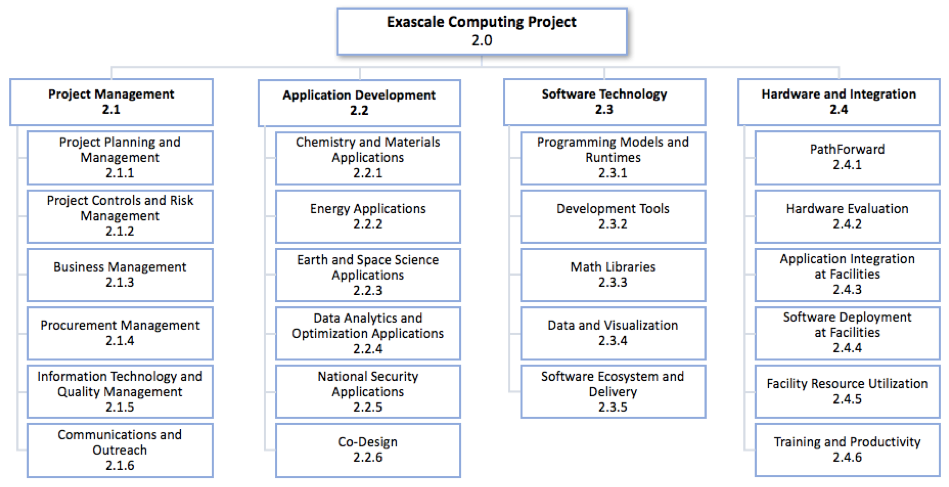
\includegraphics[width=0.9\linewidth]{ECP20}
	\caption{The ECP Work Breakdown Structure through Level 3 (L3).}
	\label{fig:ecp2}
\end{figure}

\subsection{Background}
Historically, the software used on supercomputers has come from three sources: computer system vendors, DOE laboratories, and academia. Traditionally, vendors have supplied system software:  operating system, compilers, runtime, and system-management software. The basic system software is typically augmented by software developed by the DOE HPC facilities to fill gaps or to improve management of the systems. An observation is that it is common for system software to break or not perform well when there is a jump in the scale of the system.
 
Mathematical libraries and tools for supercomputers have traditionally been developed at DOE laboratories and universities and ported to the new computer architectures when they are deployed. These math libraries and tools have been remarkably robust and have supplied some of the most impactful improvements in application performance and productivity. The challenges have been the constant adapting and tuning to rapidly changing architectures.
 
Programming paradigms and the associated programming environments that include compilers, debuggers, message passing, and associated runtimes have traditionally been developed by vendors, DOE laboratories, and universities. The same can be said for file system and storage software. An observation is that the vendor is ultimately responsible for providing a programming environment and file system with the supercomputer, but there is often a struggle to get the vendors to support software developed by others or to invest in new ideas that have few or no users yet. Another observation is that file-system software plays a key role in overall system resilience, and the difficulty of making the file-system software resilient has grown nonlinearly with the scale and complexity of the supercomputers.
 
In addition to the lessons learned from the traditional approaches, Exascale computers pose unique software challenges including the following.
\begin{itemize}
\item \textbf{Extreme parallelism:} Experience has shown that software breaks at each shift in scale. Exascale systems are predicted to have a billion-way concurrency via a combination of tasks, threads and vectorization, and more than one hundred thousand nodes. Because clock speeds have essentially stalled, the 1000-fold increase in potential performance going from Petascale to Exascale is entirely from concurrency improvements.
\item \textbf{Data movement in a deep memory hierarchy: }Data movement has been identified as a key impediment to performance and power consumption. Exascale system designs are increasing the types and layers of memory, which further challenges the software to increase data locality and reuse, while reducing data movement.
\item \textbf{Resilience:} As hardware resilience decreases due to the number of components and reduced voltage, software resilience must be developed to take up the slack and allow the Exascale system to be adaptable to component failures without the entire system crashing.  Initial concerns about resilience at the start of Exascale efforts have diminished, and the availability of non-volatile memory should dramatically improve checkpoint/restart performance.  Even so, we need to keep a focus on this issue.
\item \textbf{Power consumption:} Exascale systems have been given an aggressive power consumption goal of 20-30 MW, not much more than the power consumed by the largest systems of today. Meeting this goal will require the development of power monitoring and management software that does not exist today.
\end{itemize}
 
In addition to the software challenges imposed by the scale of Exascale computers, the following additional requirements push ECP away from the historical approaches for getting the needed software for DOE supercomputers.
\begin{itemize}
\item \textbf{2021 acceleration:} ECP has a goal of accelerating the development of the U.S. Exascale systems and enabling the first deployment by 2021. This means that the software needs to be ready sooner, and the approach of just waiting until it is ready will not work. A concerted plan that accelerates the development of the highest priority and most impactful software is needed.
\item \textbf{Productivity:} Traditional supercomputer software requires a great deal of expertise to use. ECP has a goal of making Exascale computing accessible to a wider science community than previous supercomputers have been. This requires the development of software that improves productivity and ease of use.
\item \textbf{Diversity:} There is a strong push to make software run across diverse Exascale systems. Traditionally, there has been a focus on just one new supercomputer every couple of years. ECP has a goal of enabling at least two diverse architectures, and the ECP-developed software needs to be able to run efficiently on all of them.  Some code divergence is inevitable, but careful software design, and the use of performance portability layers can minimize the amount of code targeted at a specific platform.
\item \textbf{Analytics and machine learning:} Future DOE supercomputers will need to solve emerging data science and machine learning problems in addition to the traditional modeling and simulation applications. This will require the development of scalable, parallel analytics and machine learning software that does not exist today.
\end{itemize}
 
The next section describes the approach employed by ECP ST to address the Exascale challenges.

\subsection{ECP Software Technology Approach}
ECP is taking an approach of codesign across all its principal technical areas: applications development (AD), software technology (ST), and hardware \& integration (HI). For ECP ST, this means its requirements are based on input from other areas, and there is a tight integration of the software products both within the software stack as well as with applications and the evolving hardware. 

The portfolio of projects in ECP ST is intended to address the Exascale challenges and requirements described above. We note that ECP is not developing the entire software stack for an Exascale system. For example, we expect vendors to provide the core software that comes with the system (in many cases, by leveraging ECP and other open-source efforts). Examples of vendor-provided software include operating system, file system, compilers (for C, C++, Fortran, etc.), basic math libraries, system monitoring tools, scheduler, debuggers, vendor’s performance tools, MPI (based on ECP-funded projects), OpenMP (with features from ECP-funded project), and data-centric stack components. ECP develops other, mostly higher-level software that is needed by applications and is not vendor specific. ECP-funded software activities are concerned with extreme scalability, exposing additional parallelism, unique requirements of Exascale hardware, and performance-critical components. Other software that aids in developer productivity is needed and may come from third-party open-source efforts (e.g., gdb, Valgrind).

The ST portfolio includes both ASCR and NNSA ATDM funded efforts. The MOU established between DOE-SC and NNSA has formalized this effort.  Whenever possible, ASCR and ATDM efforts are treated uniformly in ECP ST planning and assessment activities.

ST is also planning to increase integration within the ST portfolio through increased use of software components and application composition vs. monolithic application design. An important transition that ECP can accelerate is the increased development and delivery of reusable scientific software components and libraries. While math and scientific libraries have long been a successful element of the scientific software community, their use can be expanded to include other algorithms and software capabilities, so that applications can be considered more an aggregate composition of reusable components than a monolithic code that uses libraries tangentially.

To accelerate this transition, we need a greater commitment on the part of software component developers to provide reliable and portable software that users can consider to be part of the software ecosystem in much the same way users depend on MPI and compilers. At the same time, we must expect application developers to participate as clients and users of reusable components, using capabilities from components, transitioning away from (or keeping as a backup option) their own custom capabilities.

\subsubsection{The Extreme-scale Scientific Software Stack (E4S)}\label{subsubsect:e4s}
On November 8, 2018, ECP ST released version 0.1 of the Extreme-scale Scientific Software Stack, E4S (\url{http://e4s.io}).  E4S contains a collection of the software products to which ECP ST contributes.  E4S will be the primary conduit for providing easy access to ECP ST capabilities for ECP and the broader community.  E4S will also be the ECP ST vehicle for regression and integration testing across DOE pre-Exascale and Exascale systems.

\begin{figure}
		\centering
		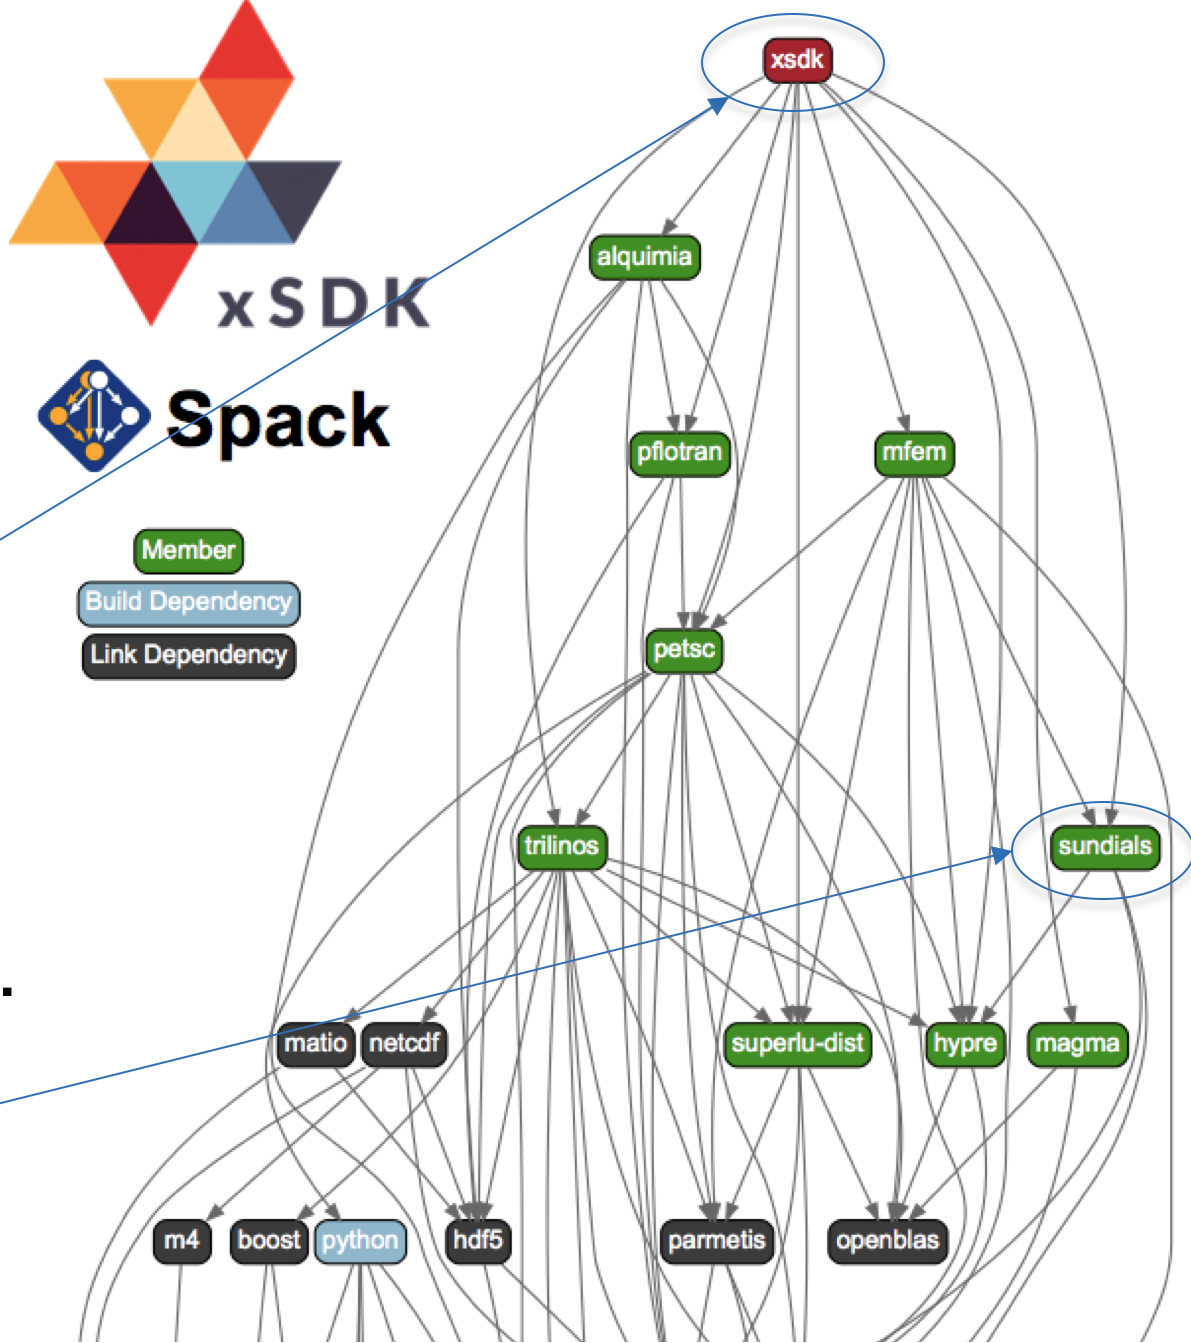
\includegraphics[scale=0.3]{E4S-Build-Tree}
	\caption{Using Spack~\cite{gamblin+:ecp18-spack-tutorial}, E4S builds a comprehensive software stack.  As ECP ST efforts proceed, we will use E4S for continuous integration testing, providing developers with rapid feedback on regression errors and providing user facilities with a stable software base as we prepare for Exascale platforms.  This diagram shows how E4S builds ECP products via an SDK target (the math libraries SDK called xSDK in this example).  The SDK target then builds all product that are part of the SDK (see Figure~\ref{fig:sdk-definition1} for SDK groupings), first defining and building external software products. Green-labeled products are part of the SDK. The blue-label indicates expected system tools, in this case a particular version of Python.  Black-labeled products are expected to be previously installed into the environment (a common requirement and easily satisified).  Using this approach, a user who is interested in only SUNDIALS (a particular math library) can be assured that the SUNDIALS build will be possible since it is a portion of what E4S builds and tests.}
	\label{fig:e4s-build-tree}
\end{figure}

E4S has the following key features:
\begin{itemize}
	\item \textbf{The E4S suite is a large and growing effort to build and test a comprehensive scientific software ecosystem:} E4S V0.1 contained 25 ECP products.  E4S V0.2, release in January 2019 contained 37 ECP products and numerous additional products needed for a complete software environment.  Eventually E4S will contain all open source products to which ECP contributes, and all related products needed for a holistic environment.
	\item \textbf{E4S is not an ECP-specific software suite:}  The products in E4S represent a holistic collection of capabilities that contain the ever-growing SDK collections sponsored by ECP and all additional underlying software required to use ECP ST capabilities.  Furthermore, we expect the E4S effort to live beyond the timespan of ECP, becoming a critical element of the scientific software ecosystem.
	\item \textbf{E4S is partitionable:} E4S products are built and tested together using a tree-based hierarchical build process.  Because we build and test the entire E4S tree, users can build any subtree of interest, without building the whole stack (see Figure~\ref{fig:e4s-build-tree}).
	\item \textbf{E4S uses Spack:} The Spack~\cite{gamblin+:ecp18-spack-tutorial} meta-build tool invokes the native build process of each product, enabling quick integration of new products, including non-ECP products.
	\item \textbf{E4S is available via containers:} In addition to a build-from-source capability using Spack, E4S maintains several container environments (Docker, Singularity, Shifter, CharlieCloud) that provides the lowest barrier to use.  Container distributions dramatically reduce installation costs and provide a ready-made environment for tutorials that leverage E4S capabilities.  For example, the ECP  application project CANDLE (Cancer Deep Learning Environment) uses an E4S container to provide a turnkey tutorial execution environment.
	\item \textbf{E4S distribution:} E4S products are available at \url{http://e4s.io}.
	\item \textbf{E4S developer community resources:} Developers interested in participating in E4S can visit the E4S-Project GitHub community at \url{https://github.com/E4S-Project}.	
\end{itemize}

The E4S effort is described in further detail in Sections~\ref{subsect:ecosystem}, especially Section~\ref{subsubsect:sdks}.

\subsubsection{Software Development Kits}\label{subsubsect:sdks}
One opportunity for a large software ecosystem project such as ECP ST is to foster increased collaboration, integration and interoperability among its funded efforts. Part of ECP ST design is the creation of software development kits (SDKs).  SDKs are collections of related software products (called packages) where coordination across package teams will improve usability and practices and foster community growth among teams that develop similar and complementary capabilities. SDKs have the following attributes:
\begin{table}
	\begin{mdframed}
\begin{enumerate}
	\item \textbf{Domain scope:} Each SDK will be composed of packages whose capabilities are within a natural functionality domain. Packages within an SDK provide similar capabilities that can enable leveraging of common requirements, design, testing and similar activities. Packages may have a tight complementary such that ready composability is valuable to the user.
	\item \textbf{Interaction models:} How packages within an SDK interact with each other. Interactions include common data infrastructure, or seamless integration of other data infrastructures; access to capabilities from one package for use in another.
	\item \textbf{Community policies:} Expectations for how package teams will conduct activities, the services they provide, software standards they follow, and other practices that can be commonly expected from a package in the SDK.
	\item \textbf{Meta-build system:} Robust tools and processes to build (from source), install and test the SDK with compatible versions of each package. This system sits on top of the existing build, install and test capabilities for each package.
	\item \textbf{Coordinated plans:} Development plans for each package will include efforts to improve SDK capabilities and lead to better integration and interoperability.
	\item \textbf{Community outreach:} Efforts to reach out to the user and client communities will include explicit focus on SDK as product suite.
\end{enumerate}
	\end{mdframed}
\caption{\label{table:sdk-attributes} Software Development Kits (SDKs) provide an aggregation of software products that have complementary or similar attributes.  ECP ST uses SDKs to better assure product interoperability and compatibility.  SDKs are also essential aggregation points for coordinated planning and testing. SDKs are an integral element of ECP ST~\cite{Heroux-SDK-Podcast}.  Section~\ref{subsubsect:ecosystem-sdk} describes the six SDK groupings and the current status of the SDK effort.}
\end{table}

\paragraph{ECP ST SDKs}
As part of the delivery of ECP ST capabilities, we will establish and grow a collection of SDKs. The new layer of aggregation that SDKs represent are important for improving all aspects of product development and delivery. The communities that will emerge from SDK efforts will lead to better collaboration and higher quality products. Established community policies will provide a means to grow SDKs beyond ECP to include any relevant external effort. The meta-build systems (based on Spack) will play an important role in managing the complexity of building the ECP ST software stack, by providing a new layer where versioning, consistency and build options management can be addressed at a mid-scope, below the global build of ECP ST products.
Each ECP ST L3 (five of them) has funds for an SDK project from which we have identified a total of six SDKs and an at-large collection of remaining products that will be delivered outside of the SDK grouping.  Section~\ref{subsubsect:ecosystem-sdk} provides an update on the progress in defining SDK groupings. For visibility, we provide the same diagram in Figure~\ref{fig:sdk-definition1-0}.

\begin{figure}[htb]
	\centering
	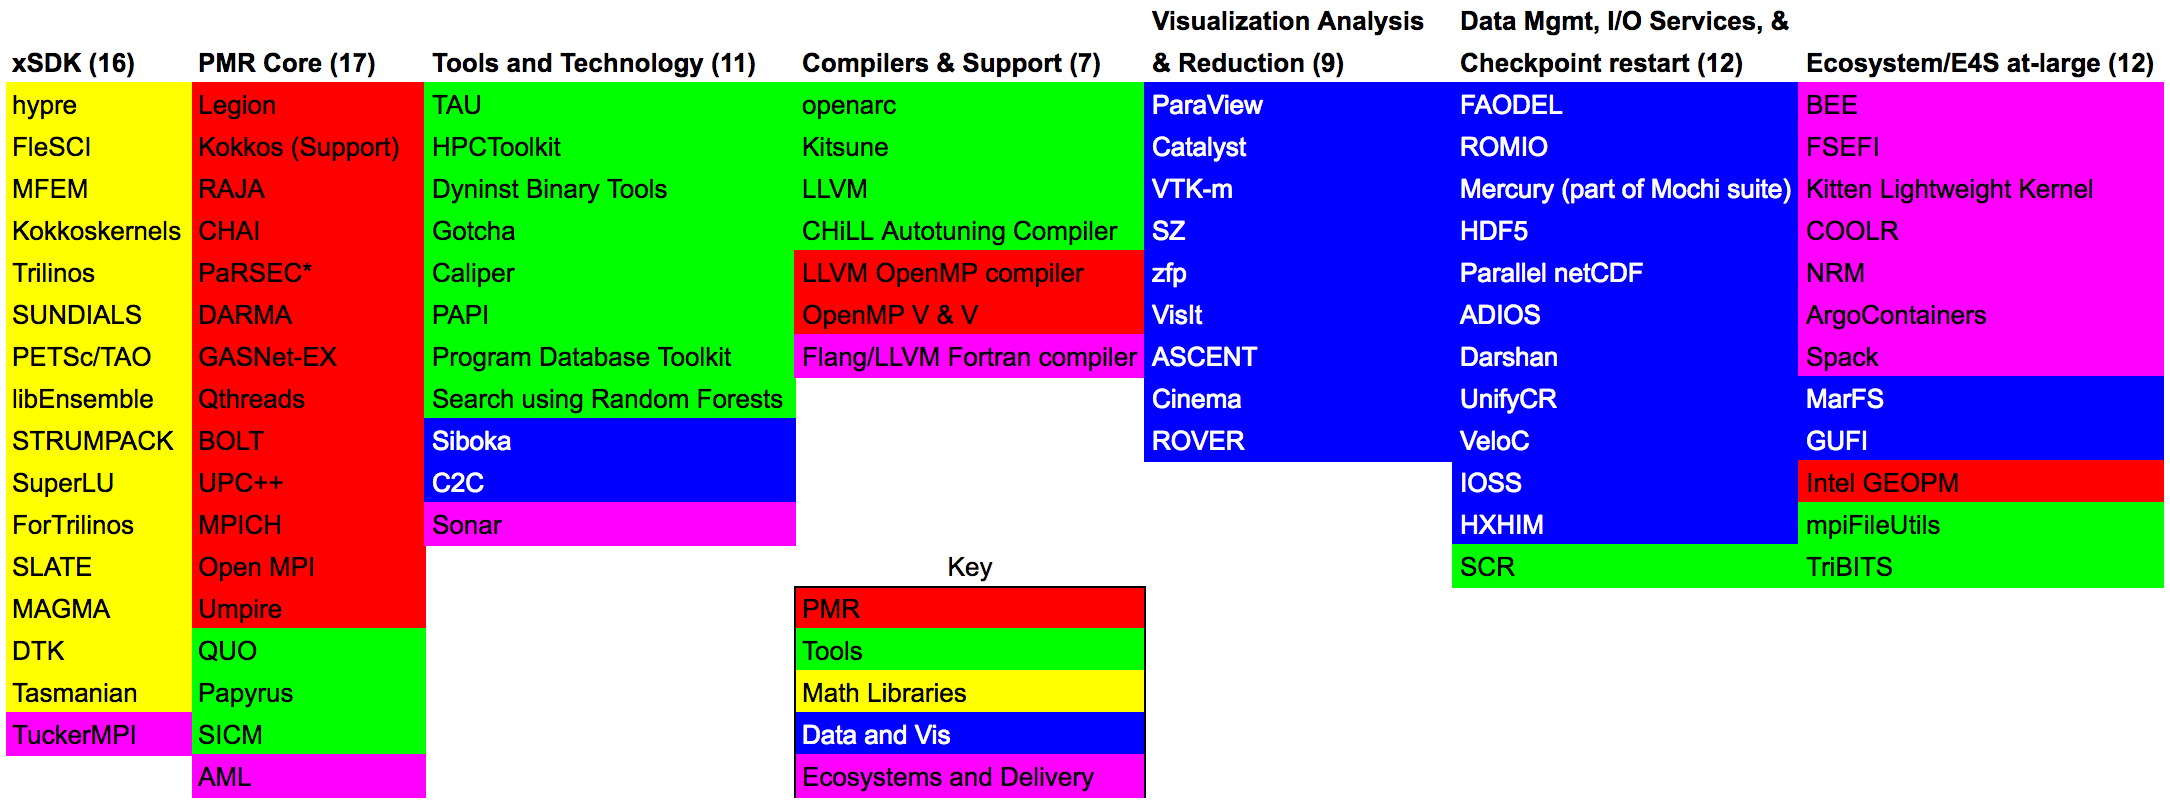
\includegraphics[width=6.5in]{projects/2.3.5-Ecosystem/2.3.5.01-Ecosystem-SDK/SDKdefinition1}
	\caption{\label{fig:sdk-definition1-0}The above graphic shows the breakdown of ECP ST products into 6 SDKs ( the first six columns).  The rightmost column lists products that are not part of an SDK, but are part of Ecosystem group that will also be delivered as part of E4S. The colors denoted in the key map all of the ST products to the ST technical area they are part of.  For example, the xSDK consists of products that are in the Math Libraries Technical area, plus TuckerMPI which is in the Ecosystem and Delivery technical area.  Section~\ref{subsubsect:ecosystem-sdk} provides an update on the progress in defining SDK groupings.}
\end{figure}


%will identify and establish at least one SDK effort. Fortunately, we will be able to leverage an existing SDK in the Math Libraries sub-element to inform our broader efforts. This SDK, called the xSDK, has been in existence for several years and has proven the value of an SDK approach in its domain (Figure~\ref{fig:xsdk-diagram}). 

%\begin{figure}
%	\centering
%	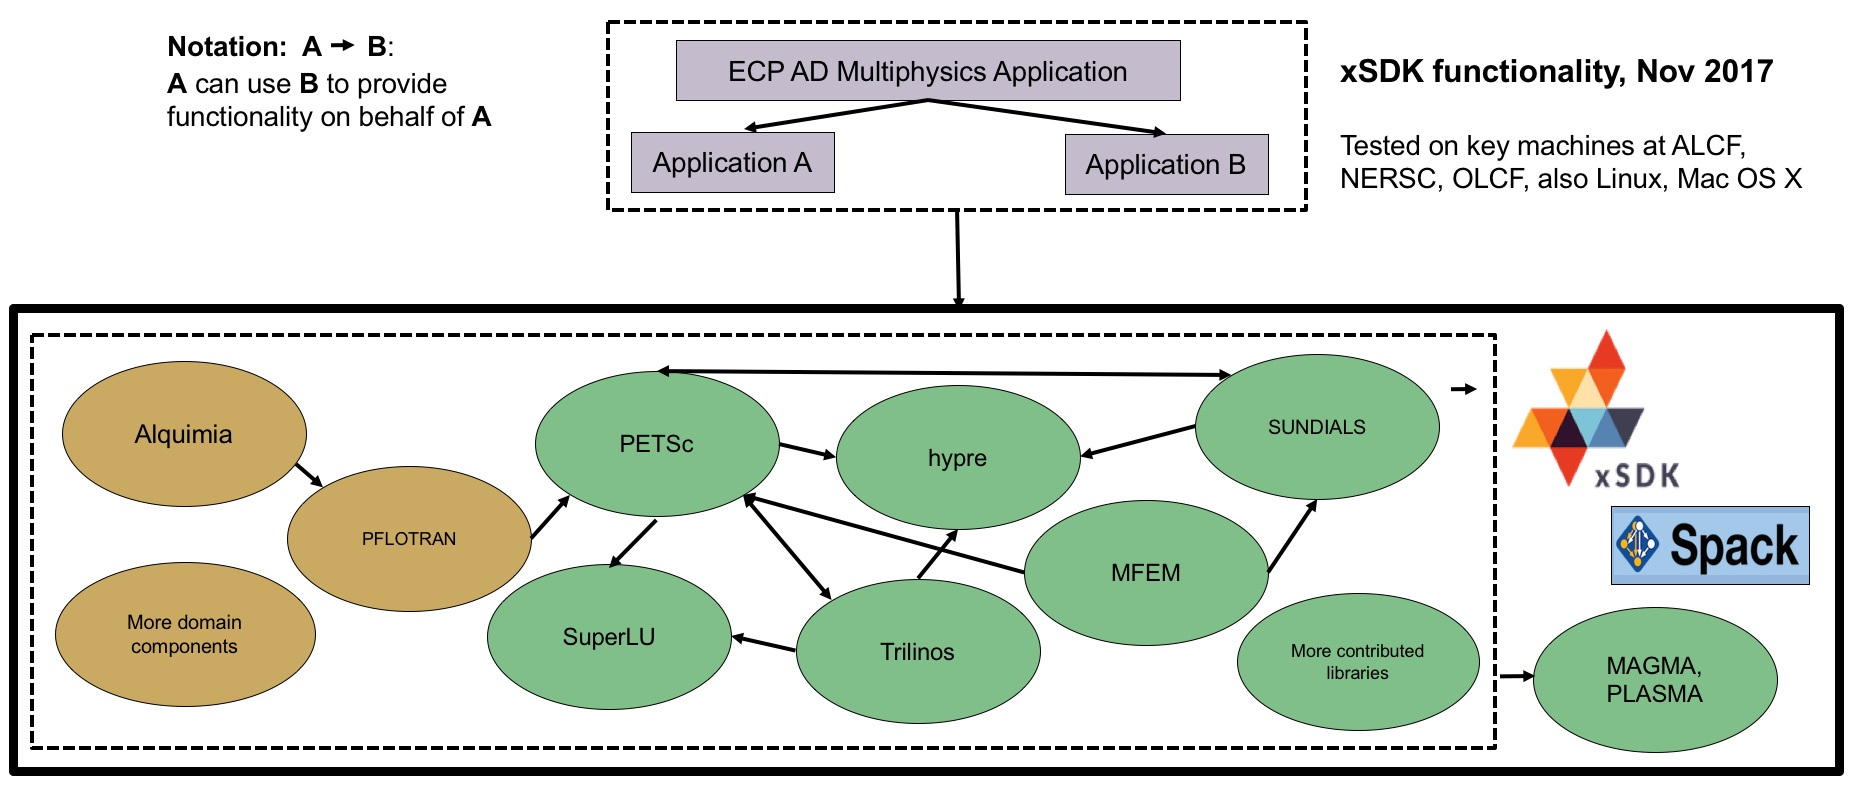
\includegraphics[width=0.9\linewidth]{xSDK-Diagram}
%	\caption{The xSDK is the first SDK for ECP ST, in the Mathematical Libraries technical area~\ref{table:wbs}. The xSDK provides the collaboration environment for improving build, install and testing capabilities for member packages such as hypre, PETSc, SuperLU and Trilinos (and other products with green background). Domain components (see orange ovals) are also an important category of the ecosystem, providing leveraged investments for common components in a specific scientific software domain.  xSDK capabilities are essential for supporting the multi-physics and multi-scale application requirement that lead to combined use of xSDK libraries. Furthermore, the availability of advanced software platforms such as GitHub, Confluence, JIRA and others enable the level of collaboration needed to create an SDK from independently developed packages.}
%	\label{fig:xsdk-diagram}
%\end{figure}
%
%
%\paragraph{The xSDK}
%Initially funded by the DOE Office of Advanced Scientific Computing Research and the office of Biological and Environmental Research as part of the IDEAS Project~\cite{Bartlett:2017:XFT:3148208.3148212}, the xSDK is a collection of independent math library packages, initially the popular libraries hypre, PETSc, SuperLU and Trilinos. The xSDK was established in recognition that collaboration across independent library development efforts could have a tremendous positive impact on the math libraries capabilities provided to users, and the productivity of library developers and sustainability of library software.
%Figure~\ref{fig:xsdk-diagram} illustrates the scope and interaction of xSDK packages and Figure~\ref{fig:xsdk-policies} lists the community policies that govern xSDK activities and set expectations for future xSDK members. While we recognize that xSDK experiences cannot be blindly applied to creation of new SDKs in ECP, the xSDK does provide a concrete, working example to guide ECP ST SDK efforts going forward.
%\begin{figure}
%	\centering
%	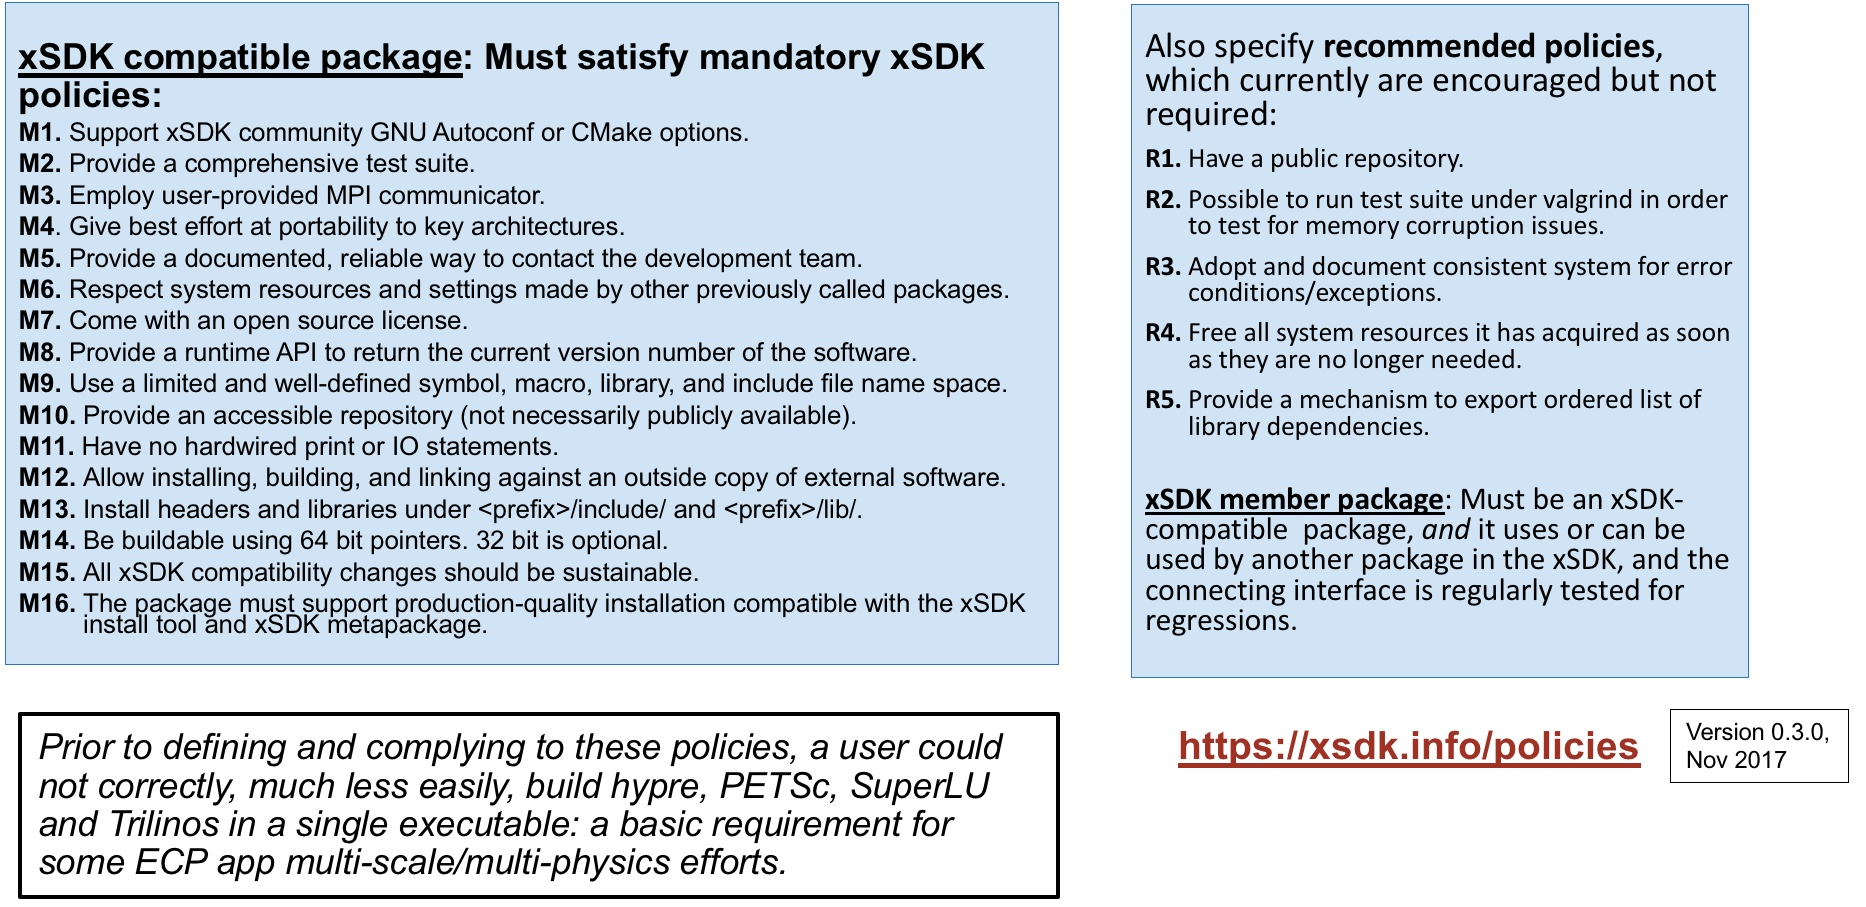
\includegraphics[width=0.9\linewidth]{xSDK-Policies}
%	\caption{\textbf{xSDK Community Policies emerged from challenging and passionate discussions about essential values of the math libraries community.} Once established, these community policies represent a living statement of what it means to be part of an SDK, and are used as the criteria for welcoming future members.}
%	\label{fig:xsdk-policies}
%\end{figure}

\subsubsection{ECP ST Software Delivery}
An essential activity for, and the ultimate purpose of, ECP ST is the delivery of a software stack that enables productive and sustainable Exascale computing capabilities for target ECP applications and platforms, and the broader high-performance computing community. The ECP ST Software Ecosystem and Delivery sub-element (WBS 2.3.5) and the SDKs in each other sub-element provide the means by which ECP ST will deliver its capabilities.
\paragraph{ECP ST Delivery and HI Deployment}
Providing the ECP ST software stack to ECP applications requires coordination between ECP ST and ECP HI. The focus areas have a complementary arrangement where ECP ST delivers its products and ECP HI deploys them. Specifically:
\begin{itemize}
	\item ST \textbf{delivers} software.  ECP ST products are delivered directly to application teams, to vendors and to facilities.  ECP ST designs and implements products to run on DOE computing facilities platforms and make products available as source code via GitHub, GitLab or some other accessible repository.
	\item HI facilitates efforts to \textbf{deploy} ST (and other) software on Facilities platforms by installing it where users expect to find it. This could be in /usr/local/bin or similar directory, or available via “module load”.
\end{itemize}
Separating the concerns of delivery and deployment is essential because these activities require different skill sets. Furthermore, ECP ST delivers its capabilities to an audience that is beyond the scope of specific Facilities’ platforms. This broad scope is essential for the sustainability of ECP ST products, expanding the user and developer communities needed for vitality. In addition, ECP HI, the computer system vendors and other parties provide deployable software outside the scope of ECP ST, therefore having the critical mass of skills to deploy the entire software stack.

\paragraph{ECP ST Delivery Strategy}
ECP ST delivers it software products as source code, primarily in repositories found on GitHub, Gitlab installations or similar platforms. Clients such as ECP HI, OpenHPC and application developers with direct repository access then take the source and build, install and test our software. The delivery strategy is outlined in Figure~\ref{fig:softwarestack}.  

Users access ECP ST products using these basic mechanisms (see Figure~\ref{fig:productsoverview} for deliverable statistics):
\begin{itemize}
	\item \textbf{Build from source code:} The vast majority of ECP ST products reach at least some of their user base via direct source code download from the product repository.  In some cases, the user will download a single compressed file containing product source, then expand the file to expose the collection of source and build files.  Increasingly, users will fork a new copy of an online repository.  After obtaining the source, the user executes a configuration process that detects local compilers and libraries and then builds the product.  This kind of access can represent a barrier for some users, since the user needs to build the product and can encounter a variety of challenges in that process, such as an incompatible compiler or a missing third-party library that must first be installed.  However, building from source can be a preferred approach for users who want control over compiler settings, or want to adapt how the product is used, for example, turning on or off optional features, or creating adaptations that extend product capabilities.  For example, large library frameworks such as PETSc and Trilinos have many tunable features that can benefit from the user building from source code.  Furthermore, these frameworks support user-defined functional extensions that are easier to support when the user builds the product from source.  ECP ST is leveraging and contributing to the development of Spack~\cite{gamblin+:sc15}.  Via meta-data stored in a Spack \textit{package} defined for each product, Spack leverages a product's native build environment, along with knowledge about its dependencies, to build the product and dependencies from source.  Spack plays a central role in ECP ST software development and delivery processes by supporting turnkey builds of the ECP ST software stack for the purposes of continuous integration testing, installation and seamless multi-product builds.
	\item \textbf{DOE computing facilities:} Each DOE computing facility (ALCF, OLCF, NERSC, LLNL and ACES [LANL/SNL]) provides pre-built versions of 17 to 20 ECP ST products (although the exact mix of products varies somewhat at each site).  Many of these products are what users would consider to be part of the core system capabilities, including compilers, e.g., Flang (Section~\ref{subsubsect:flang}) and LLVM (Section~\ref{subsubsect:sollve}), and parallel programming environments such as MPICH (Section~\ref{subsubsect:mpich}), OpenMPI (Section~\ref{subsubsect:openmpi}) and OpenMP (Section~\ref{subsubsect:bolt}).  Development tools such as PAPI (Section~\ref{subsubsect:exapapi}) and TAU (Section~\ref{subsubsect:tau}) are often part of this suite, if not already included in the vendor stack. Math and data libraries such as PETSc (Section~\ref{subsubsect:petsc}), Trilinos (Section~\ref{subsubsect:trilinos}), HDF5 (Section~\ref{subsubsect:exahdf5}) and others are also available in some facilities software installations.  We anticipate and hope for increased collaboration with facilities via the ECP Hardware \& Integration (HI) Focus Area.  We are also encouraged by multi-lab efforts such as the Tri-Lab Operating System Stack (TOSS)~\cite{TOSS} that are focused on improving uniformity of software stacks across facilities.
	\item \textbf{Vendor stacks:} Computer system vendors leverage DOE investments in compilers, tools and libraries.  Of particular note are the wide use of MPICH(Section~\ref{subsubsect:mpich}) as software base for most HPC vendor MPI implementations and the requirements, analysis, design and prototyping that ECP ST teams provide.  Section~\ref{subsection:external-contributions} describes some of these efforts.
	\item \textbf{Binary distributions:} Approximately 10 ECP ST products are available via binary distributions such as common Linux distributions, in particular via OpenHPC\cite{OpenHPC}.  ECP ST intends to foster growth of availability via binary distributions as an important way to increase the size of the user community and improve product sustainability via this broader user base.
\end{itemize}

\begin{figure}
	\centering
	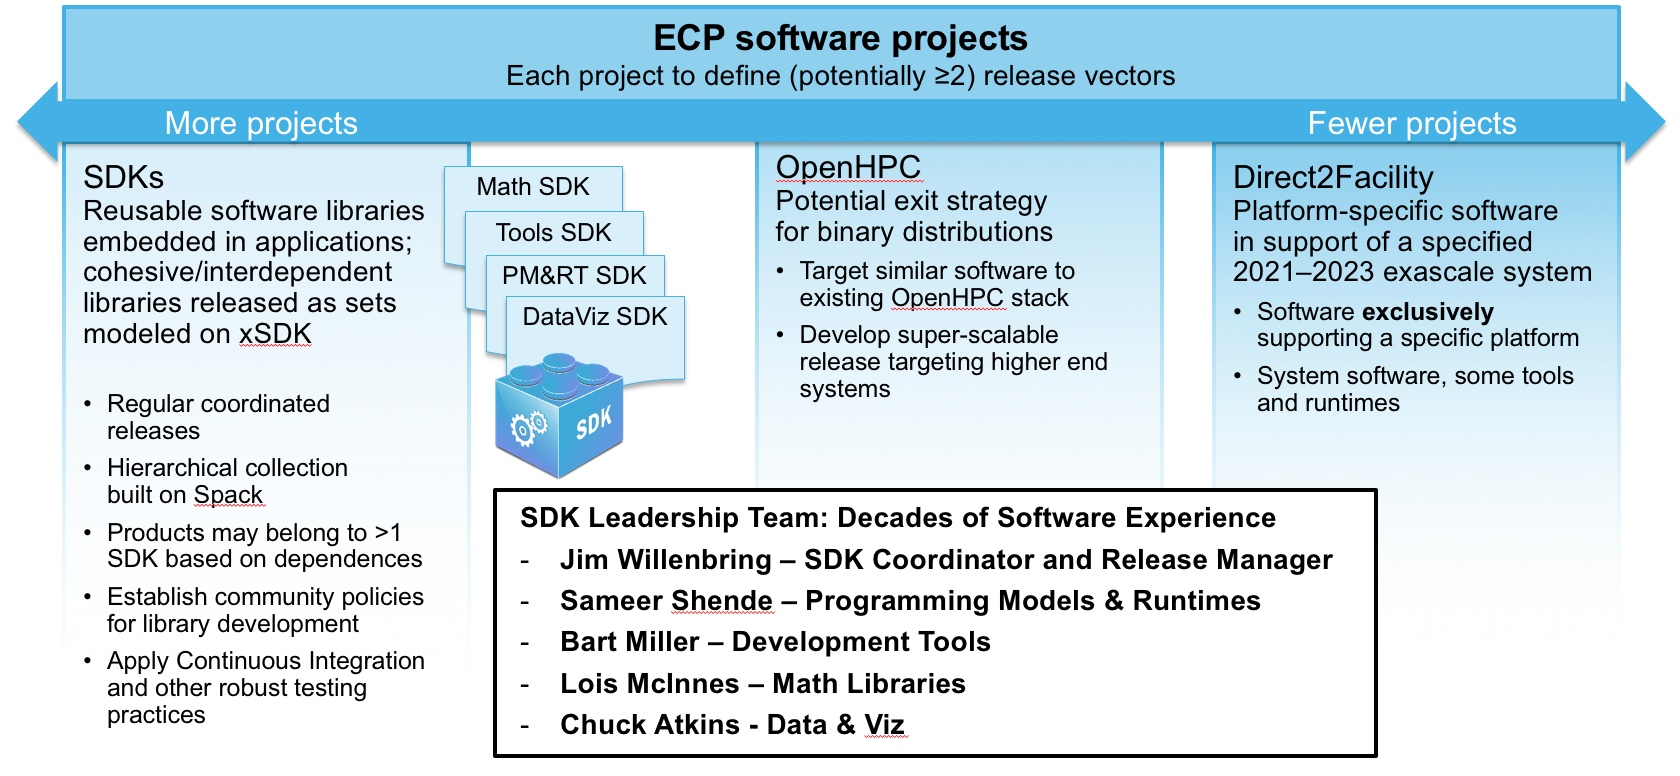
\includegraphics[width=0.9\linewidth]{SoftwareStack}
	\caption{\textbf{The ECP ST software stack is delivered to the user community through several channels.} Key channels are via source code, increasing using SDKs, direct to Facilities in collaboration with ECP HI, via binary distributions, in particular the OpenHPC project and via HPC vendors.  The SDK leadership team includes  ECP ST team members with decades of experience delivering scientific software products.}
	\label{fig:softwarestack}
\end{figure}

\subsection{ECP ST Project Restructuring}\label{subsect:ProjectRestructuring}

The initial organization of ECP ST was based on discussions that occurred over several years of Exascale planning within DOE, especially the DOE Office of Advanced Scientific Computing Research (ASCR).  Figure~\ref{fig:ecpstv1} shows the conceptual diagram of this first phase.  The 66 ECP ST projects were mapped into 8 technical areas, in some cases arbitrating where a project should go based on its primary type of work, even if other work was present in the project.  In November 2017, ECP ST was reorganized into 5 technical areas, primarily through merging a few smaller areas, and the number of projects was reduced to 56 (presently 55 due to further merging in \ecosystem).  Figure~\ref{fig:ecpstv2} shows the diagram of the second phase of ECP ST.  With the CAR V2.0, we will describe the next phase of organization refinement needed to best position ECP ST for success in the CD-2 phase of the project.

\begin{table}
\begin{tabular}{|L{1in}|L{1in}|L{1.0in}|L{2.5in}|}\hline
\textbf{WBS} & \textbf{Role/Area} & \textbf{Leader} & \textbf{Transition} \\\hline
1.3 & ECP ST Director & Rajeev Thakur & Renumbered to 2.3.  Thakur left director role, continues as lead of 2.3.1 \pmr. Mike Heroux new director. \\\hline
1.3 & ECP ST Deputy Director & Pat McCormick & McCormick left deputy role, continued as PI of 2.3.1.08 Legion project. Jonathan Carter new deputy director.\\\hline
1.3.1 & Programming Models \& Runtimes & Rajeev Thakur& Renumbered to 2.3.1, renamed to \pmr, otherwise unchanged. \\\hline
1.3.2 & Tools & Jeffrey Vetter
& Renumbered to 2.3.2, renamed to \tools, otherwise unchanged. \\\hline
1.3.3 & Math/Scientific Libs & Mike Heroux & New leader Lois Curfman McInnes, renamed Mathematical Libraries, new number 2.3.3. \\\hline
1.3.4 & Data Management \& Workflows & Rob Ross & Combined with 1.3.5 to create 2.3.4. Jim Ahrens leader. \\\hline
1.3.5 & Data Analytics \& Visualization & Jim Ahrens
& Combined with 1.3.4 to create 2.3.4. Jim Ahrens leader.\\\hline
1.3.6 & System Software & Martin Schulz& Combined with 1.3.7 and 1.3.8 into 2.3.5. Rob Neely leader.\\\hline
1.3.7 & Resilience & Al Geist & Combined with 1.3.6 and 1.3.8 into 2.3.5. Rob Neely leader. \\\hline
1.3.8 & Integration & Rob Neely & 
Combined with 1.3.6 and 1.3.7 into 2.3.5. Rob Neely leader. \\\hline
\end{tabular}
	\caption{\label{fig:wbs-transition}ECP ST technical areas were reduced from 8 to 5 in November 2017.  This figure shows how areas were remapped and merged.  In addition, the ECP ST Director and Deputy Director changed from Rajeev Thakur (who continues as the \pmr\ lead) and Pat McCormick to Mike Heroux and Jonathan Carter, respectively.}
\end{table}

\begin{figure}
\begin{mdframed}
\begin{itemize}
\item Phase 1: 66 total projects
\begin{itemize}
\item 35 projects funded by the DOE Office of Science that were selected in late 2016 via an RFI and RFP process, considering prioritized requirements of applications and DOE facilities. 
These projects started work in January–March 2017 depending on when the contracts were awarded.
\item 31 ongoing DOE NNSA funded projects that are part of the Advanced Technology Development and Mitigation (ATDM) program. The ATDM program started in FY14.  These projects are focused on longer term research to address the shift in computing technology to extreme, heterogeneous architectures and to advance the capabilities of NNSA simulation codes.
\end{itemize}
\item Phase 2: 56 total projects
(now 55 after further merging in 2.3.5)
\begin{itemize}
\item 41 ASCR-funded projects.  Added  2 \ecosystem\ projects and 4 SDK projects.
\item 15 ATDM projects: Combined the previous 31 ATDM projects into one project per technical area per lab.  ATDM projects are generally more vertically integrated and would not perfectly mapped to any proposed ECP ST technical structure.  Minimizing the number of ATDM projects within the ECP WBS structure reduces complexity of ATDM to ECP coordination and gives ATDM flexibility in revising its portfolio without disruption to the ECP-ATDM mapping.
\end{itemize}
\item Phase 3: Fewer, larger and more uniform-sized projects
\begin{itemize}
	\item Starting with FY2020, ECP ST will further consolidate L4 projects to foster additional synergies and amortize project overheads as ECP heads into Critical Decision Phase 2~\cite{413.3B}, where more rigor in planning and execution are needed.
	\item Details of this plan are available to project stakeholders in the CAR V1.5 appendix and will be in the public portion of the CAR V2.0 in July 2019.
\end{itemize}
\end{itemize}
\end{mdframed}

\caption{\label{fig:project-remapping}Project remapping summary from Phase 1 (through November 2017) to Phase 2 (After November 2017) to Phase 3 (After October 1, 2019)}
\end{figure}


\begin{figure}
	\centering
	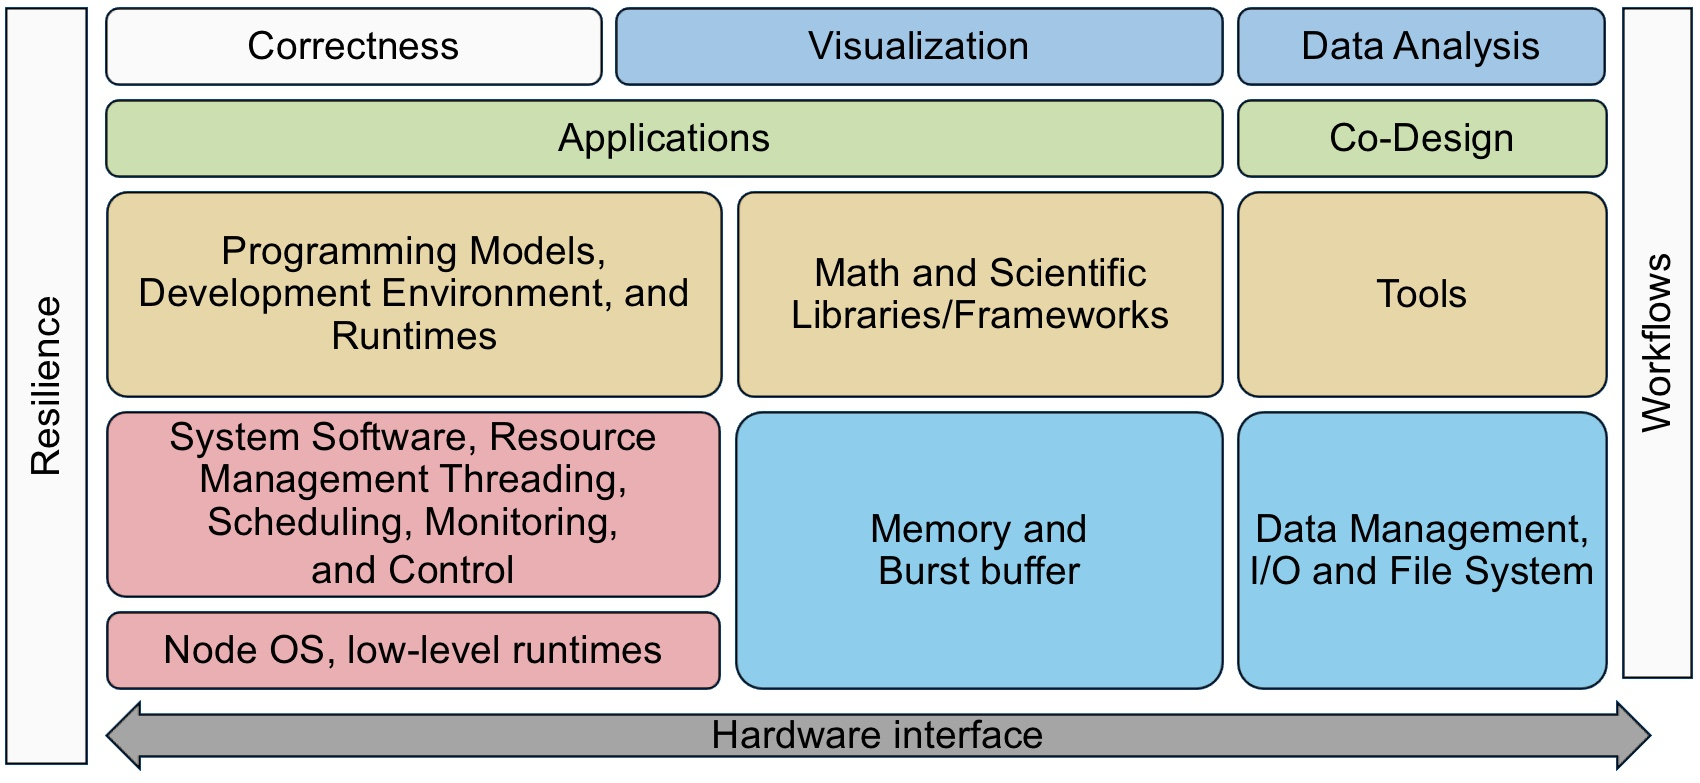
\includegraphics[width=0.9\linewidth]{ECPSTV1}
	\caption{ECP ST before November 2017 reorganization.  This conceptually layout emerged from several years of Exascale planning, conducted primarily within the DOE Office of Advanced Scientific Computing Research (ASCR).  After a significant restructuring of ECP that removed much of the facilities activities and reduced the project timeline from 10 to seven years, and a growing awareness of what risks had diminished, this diagram no longer represented ECP ST efforts accurately.}
	\label{fig:ecpstv1}
\end{figure}
\begin{figure}
	\centering
	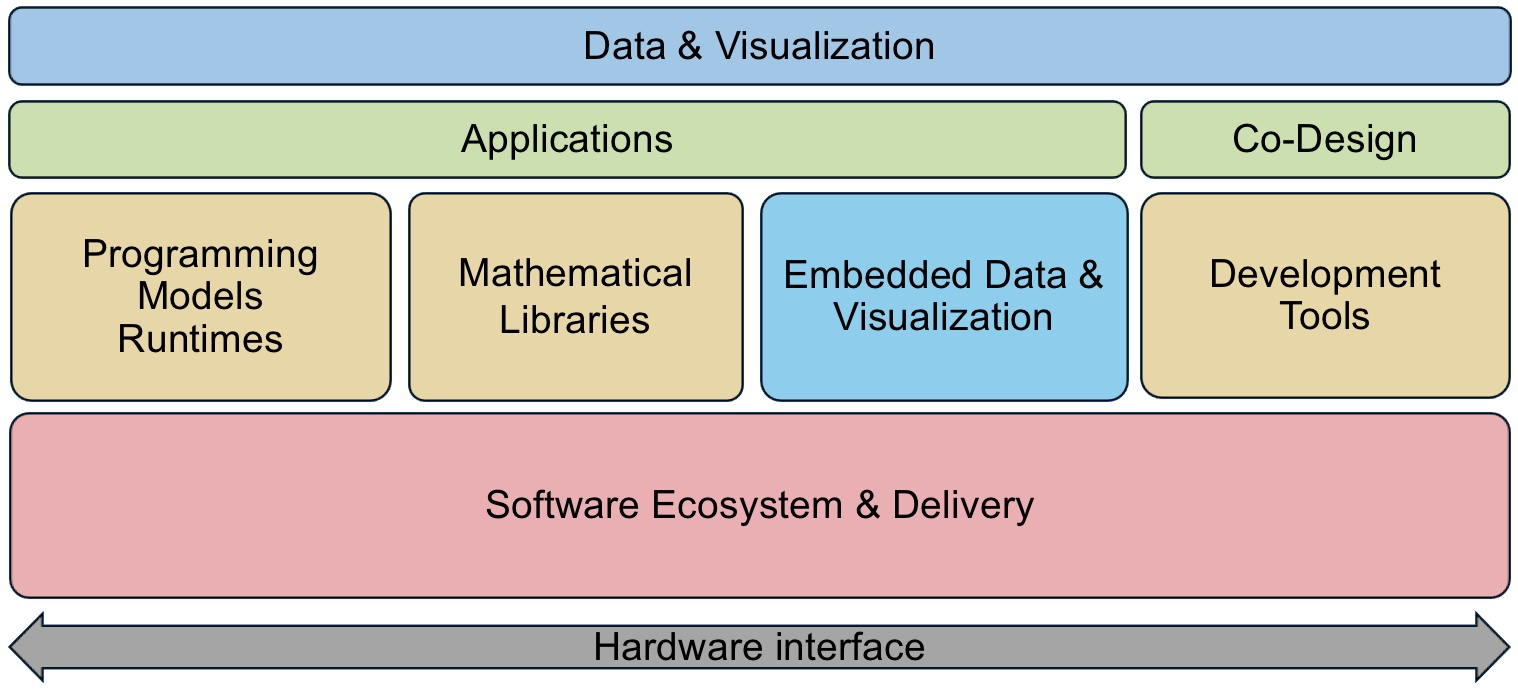
\includegraphics[width=0.9\linewidth]{ECPSTV2}
	\caption{ECP ST after November 2017 reorganization.  This diagram more accurately reflects the priorities and efforts of ECP ST given the new ECP project scope and the demands that we foresee.}
	\label{fig:ecpstv2}
\end{figure}
\begin{figure}
	\centering
	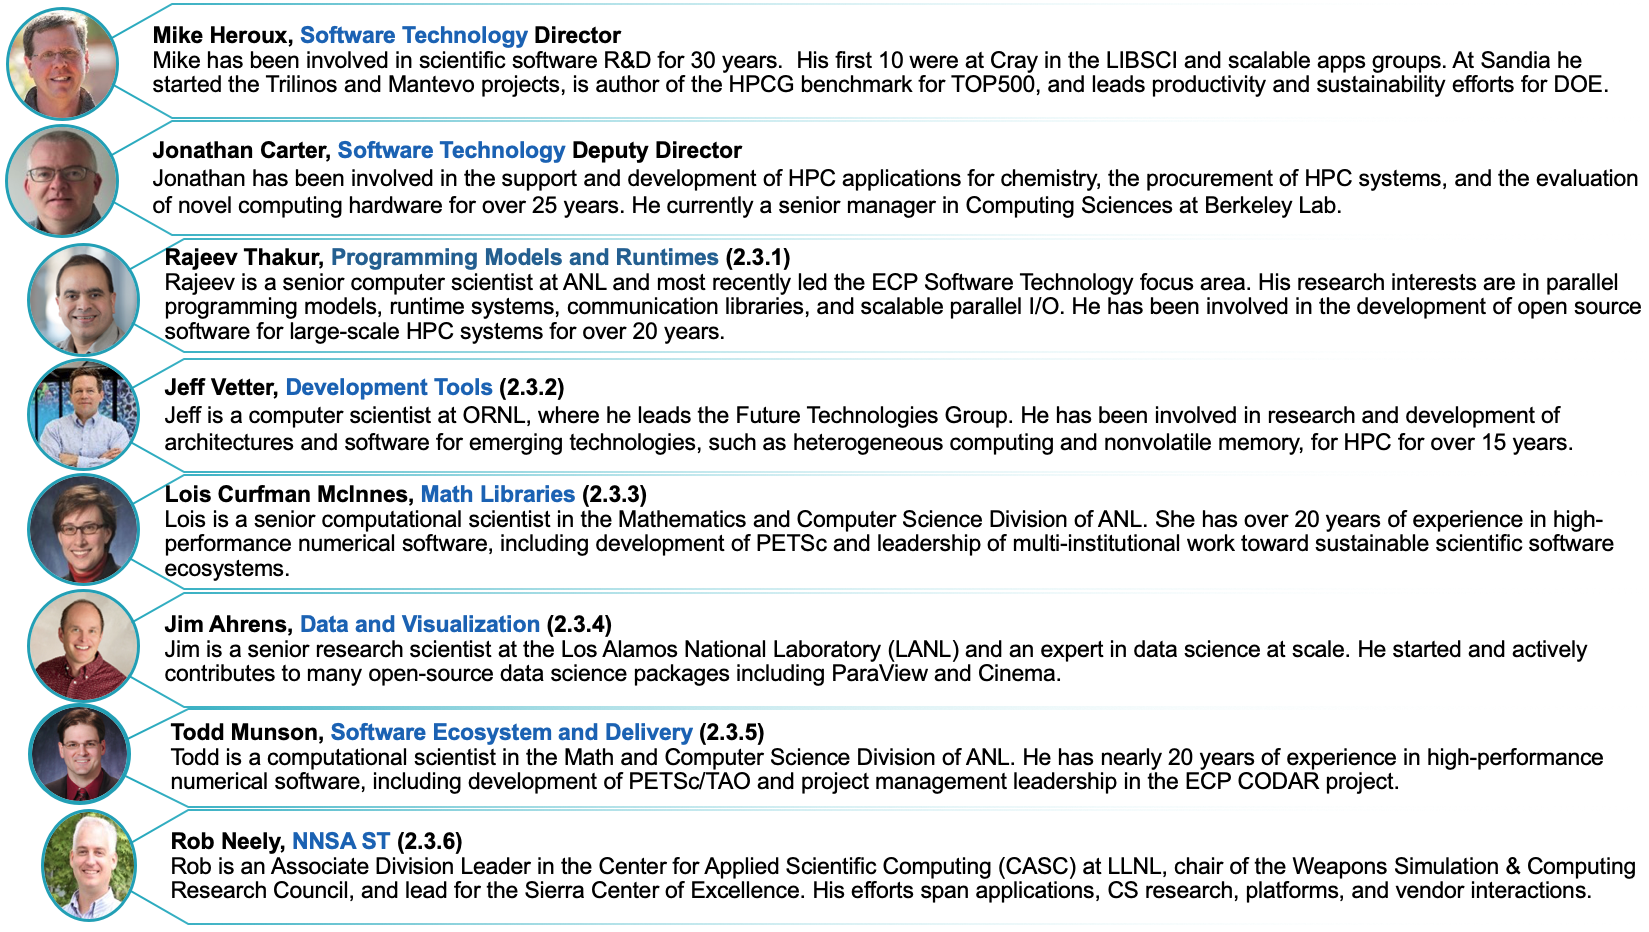
\includegraphics[width=0.9\linewidth]{ECP-ST-Leads}
	\caption{ECP ST Leadership Team as of November 2017.}
	\label{fig:ecpstleads}
\end{figure}

%\subsection{New Project Efforts}
%ECP ST is preparing several strategic changes for the FY2020 restructuring (Phase 3).   These changes will be reported in the CAR V2.0.  No other significant changes have been made since the CAR V1.0.


%\subsubsection{FFTs}\label{subsubsect:ffts}
%ECP ST has initiated two new efforts in Fast Fourier Transforms (FFTs).  FFTs provide an essential mathematical tool to many application areas.  From the very beginning of HPC, vendors have provided optimized FFT libraries for their users.  The advent of FFTW~\cite{FFTW05}, a tunable high-performance library with a well-designed interface, enabled a \textit{de facto} standardization of FFT interfaces, and an effective source base for vendor libraries, which adapted FFTW source for their platforms.
%
%There is some concern in the community that FFTW is no longer actively developed, nor well prepared for emerging platforms.  Furthermore, FFTW's strong copylefting license (which forces its users to make their own software open source in the same way) has always been a challenge to users.  While vendors are still committed to providing optimized FFT libraries, whether or not FFTW is available, we believe it is prudent to explore a new software stack and have funded a short-term project to explore this possibility.  The new library will also explore problem formulations that could significantly reduce the computational cost of FFTs.  This new effort, called FFTX, will be led by Lawrence Berkeley National Lab, under the existing math libraries project (Section~\ref{subsubsect:strumpack}).
%
%A second FFT project will address a consensus opportunity to provide a sustainable 3D FFT library built from established but \textit{ad hoc} software tools that have traditionally been part of application codes, but not extracted as independent, supported libraries.  These 3D FFTs rely on third-party 1D FFTs, either from FFTW or from vendor libraries.
%
%The goal of this second project, FFT-ECP, led by the University of Tennessee and integrated into one of its existing projects (Section~\ref{subsubsect:slate}) is to:
%\begin{itemize}
%\item Collect existing FFT capabilities recently made available from ECP application teams (LAMMPS/fftMPI and HACC/SWFFT). 
%\item Assess gaps and make available as a sustainable math library.
%\item Explore opportunities to build 3D FFT libraries on vendor 1D and 2D kernels, especially leveraging on-node concurrency from 2D and batched 1D formulations.
%\item Focus on capabilities for Exascale platforms.
%\item Emphasize leverage of vendor capabilities and addressing vendor deficiencies over creation of new and independent software stack.
%\end{itemize}
%
%This effort, while not addressing the concerns about FFTW directly, is essential to providing a new and sustainable FFT software stack that leverages the large investment by the broader HPC community in FFT software.  The payoff from this effort is almost guaranteed.  Also, should the FFTX project also go forward, it will provide an FFTW-compatible interface that would allow FFT-ECP to use FFTX as one option, in addition to external FFT libraries.
%
%\subsubsection{LLNL Math Libraries}\label{subsubsect:llnl-math-libs}
%When ECP ST started, some important capabilities were not part of the original portfolio, even though their engagement is essential for ECP application success.  This is true of the LLNL math library \textit{hypre}~\cite{hypre}.  This library is widely used to provide scalable multigrid preconditioners across several ECP applications.  Funding to support adaptation of \textit{hypre}  in preparation for Exascale platforms at science lab facilities, e.g., Argonne, and for ECP science applications was not part of the original ECP ST portfolio.  We have added funding for this effort, starting in June 2018.  In addition, we provided new funding for another LLNL math library, MFEM~\cite{mfem:homepage}, so that the MFEM team can participate in SDK efforts for math libraries.

\newpage
\section{ECP ST Technical Areas}
\subsection{\stid{1}  \pmr}

\textbf{End State:} A cross-platform, production-ready programming environment that enables and accelerates the development of mission-critical software at both the node and full-system levels.

\subsubsection{Scope and Requirements}
A programming model provides the abstract design upon which developers express and coordinate the efficient parallel execution of their program. A particular model is implemented as a developer-facing interface and a supporting set of runtime layers. To successfully address the challenges of exascale computing, these software capabilities must address the challenges of programming at both the node- and full-system levels. These two targets must be coupled to support multiple complexities expected with exascale systems (e.g., locality for deep memory hierarchies, affinity for threads of execution, load balancing) and also provide a set of mechanisms for performance portability across the range of potential and final system designs. Additionally, there must be mechanisms for the interoperability and composition of multiple implementations (e.g., one at the system level and one at the node level). This must include abilities such as resource sharing for workloads that include coupled applications, supporting libraries and frameworks, and capabilities such as in situ analysis and visualization. 

Given the ECP’s timeline, the development of new programming languages and their supporting infrastructure is infeasible. We do, however, recognize that the augmentation or extension of the features of existing and widely used languages (e.g., C/C++ and Fortran) could provide solutions for simplifying certain software development activities. 

\subsubsection{Assumptions and Feasibility}
The intent of the PMR L3 is to provide a set of programming abstractions and their supporting implementations that allow programmers to select from options that meet demands for expressiveness, performance, productivity, compatibility, and portability. It is important to note that, while these goals are obviously desirable, they must be balanced with an additional awareness that today’s methods and techniques may require changes in both the application and the overall programming environment and within the supporting software stack.

\subsubsection{Objectives}
PMR provides the software infrastructure necessary to enable and accelerate the development of HPC applications that perform well and are correct and robust, while reducing the cost both for initial development and ongoing porting and maintenance. PMR activities need to reflect the requirements of increasingly complex application scenarios, usage models, and workflows, while at the same time addressing the hardware challenges of increased levels of concurrency, data locality, power, and resilience. The software environment will support programming at multiple levels of abstraction that includes both mainstream as well as alternative approaches if feasible in ECP’s timeframe. 

Both of these approaches must provide a portability path such that a single application code can run well on multiple types of systems, or multiple generations of systems, with minimal changes. The layers of the system and programming environment implementation will therefore aim to hide the differences through compilers, runtime systems, messaging standards, shared-memory standards, and programming abstractions designed to help developers map algorithms onto the underlying hardware and schedule data motion and computation with increased automation.
\subsubsection{Plan}
PMR contains nine L4 projects. To ensure relevance to DOE missions, these efforts leverage and collaborate with existing activities within the broader HPC community. The PMR area supports the research and development needed to produce exascale-ready versions of the Message Passing Interface (MPI);  Partitioned Global-Address Space Libraries (UPC++, GASNet); task-based programming models (Legion, PaRSEC); software for node-level performance portability (Kokkos, RAJA); and libraries for memory, power, and resource management.
Initial efforts focused on identifying the core capabilities needed by the selected ECP applications and components of the software stack, identifying shortcomings of current approaches, establishing performance baselines of existing implementations on available petascale and prototype systems, and the re-implementation of the lower-level capabilities of relevant libraries and frameworks. These efforts provided demonstrations of parallel performance of algorithms on pre-exascale, leadership-class machines--at first on test problems, but eventually in actual applications (in close collaboration with the AD and HI teams). Initial efforts also informed research into exascale-specific algorithms and requirements that will be implemented across the software stack. The supported projects targeted and implemented early versions of their software on CORAL, NERSC and ACES pre-exascale systems--with an ultimate target of production-ready deployment on the exascale systems.
In FY20--23, the focus will be on development and tuning for the specific architectures of the selected exascale platforms, in addition to tuning specific features that are critical to ECP applications.

Throughout the effort, the applications teams and other elements of the software stack evaluate and provide feedback on their functionality, performance, and robustness. Progress towards these goals is documented quarterly and evaluated annually (or more frequently if needed) based on PMR-centric milestones as well as joint milestone activities shared across associated software stack activities by Application Development and Hardware \& Integration focus areas.


\subsubsection{Risks and Mitigation Strategies}
The mainstream activities of PMR focus on advancing the capabilities of the Message Passing Interface (MPI) and OpenMP. Pushing them as far as possible into the exascale era is key to supporting an evolutionary path for applications. This is the primary risk mitigation approach for both PMR and existing application codes. Extensions to MPI and OpenMP standards require research, and part of the efforts will focus on rolling these findings into existing standards, which takes time. To further address risks, PMR is exploring alternative approaches to mitigate the impact of potential limitations of the MPI and OpenMP programming models. This effort is tracked using the risk register.

Another risk is the failure of adoption of the software stack by the vendors, which is tracked in the risk register, and mitigated by the specific delivery focus in sub-element SW Ecosystems and Delivery. Past experience has shown that a combination of laboratory-supported open source software and vendor-optimized solutions built around standard APIs that encourage innovation across multiple platforms is a viable approach and what we are doing in PMR. We are using close interaction with the vendors early on to encourage adoption of the software stack, including well-tested practices of including support for key software products or APIs into large procurements through NRE or other contractual obligations. A mitigation strategy for this approach involves building a long-lasting open source community around projects that are supported via laboratory and university funding. This approach is being extended to other APIs and alternative models (that are being defined and eventually standardized) to allow for deeper and stack-wide introspection as well as resource sharing.

Creating a coordinated set of software requires strong management to ensure that duplication of effort is minimized. This is recognized by ECP management, and processes are in place to ensure collaboration is effective, shortcuts are avoided unless necessary, and an agile approach to development is instituted to prevent prototypes moving directly to product. The duplication of effort specifically, and the overall integration of the software stack, are tracked in the risk register. 

\subsubsection{Future Trends}

\subsection{\stid{2} \tools}

\textbf{End State:}	A suite of development tools and supporting unified infrastructure aimed at improving developer productivity across increasingly complex architectures, especially those targeted for Exascale platforms.


\subsubsection{Scope and Requirements}
For Exascale systems, the compilers, profilers, debuggers, and other software development tools must be increasingly sophisticated to give software developers insight into the behavior of not only the application and the underlying hardware but also the details corresponding to the underlying programming model implementation and supporting runtimes (e.g., capturing details of locality and affinity). These capabilities should be enhanced with further integration into the supporting compiler infrastructure and lower layers of the system software stack (e.g., threading, runtime systems, and data transport libraries), and hardware support. Most of the infrastructure will be released as open source, as many of them already are, with a supplementary goal of transferring the technology into commercial products. Given the diversity of Exascale systems architectures, some subset of the tools may be specific to one or more architectural features and is potentially best implemented and supported by the vendor; however, the vendor will be encouraged to use open APIs to provide portability, additional innovation, and integration into the tool suite and the overall software stack.


\subsubsection{Assumptions and Feasibility }

The overarching goal of improving developer productivity for Exascale platforms introduces new issues of scale that will require more lightweight methods, hierarchical approaches, and improved techniques to guide the developer in understanding the characteristics of their applications and to discover sources of the errors and performance issues. Additional efforts for both static and dynamic analysis tools to help identify lurking bugs in a program, such as race conditions, are also likely needed. The suite of needed capabilities spans interfaces to hardware-centric resources (e.g., hardware counters, interconnects, and memory hierarchies) to a scalable infrastructure that can collect, organize, and distill data to help identify performance bottlenecks and transform them into an actionable set of steps and information for the software developer. Therefore, these tools share significant challenges due to the increase in data and the resulting issues with management, storage, selection, analysis, and interactive data exploration. This increased data volume stems from multiple sources, including increased concurrency, processor counts, additional hardware sensors and counters on the systems, and increasing complexity in application codes and workflows.

Compilers obviously play a fundamental role in the overall programming environment but can also serve as a powerful entry point for the overall tool infrastructure. In addition to optimizations and performance profiling, compiler-based tools can help with aspects of correctness, establishing connections between programming model implementations and the underlying runtime infrastructures, and auto-tuning. In many cases, today's compiler infrastructure is proprietary and closed source, limiting the amount of flexibility for integration and exploration into the Exascale development environment. In addition to vendor compiler options, this project aims to provide an open source compiler capability that can play a role in better supporting and addressing the challenges of programming at Exascale. 


\subsubsection{Objectives}

This project will design, develop, and deploy an Exascale suite of development tools built on a unified infrastructure for development, analysis, and optimization of applications, libraries, and infrastructure from the programming environments of the project. The overarching goal is to leverage and integrate the data measurement, acquisition, storage, and analysis and visualization techniques being developed in other projects of the software stack. The project will seek to leverage techniques for common and identified problem patterns and create new techniques for data exploration related to profiling and debugging and support advanced techniques such as autotuning and compiler integration. We will seek to establish an open-source compiler activity leveraging activities around the LLVM infrastructure. These efforts will require collaboration and integration with system monitoring and various layers within the software stack.


\subsubsection{Plan}
It is expected that multiple projects will be supported under the tools effort. To ensure relevance to DOE missions, most of these efforts shall be DOE laboratory led and leverage and collaborate with existing activities within the broader HPC community. Initial efforts will focus on identifying the core capabilities needed by the selected ECP applications, components of the software stack, expected hardware features, and the selected industry activities from within the Hardware and Integration focus area. The supported projects will target and implement early versions of their software on both CORAL and APEX systems, with an ultimate target of production-ready deployment on the Exascale systems. Throughout this effort the applications teams and other elements of the software stack will evaluate and provide feedback on their functionality, performance, and robustness. These goals will be evaluated yearly (or more often as needed) based on milestones as well as joint milestone activities shared across the associated software stack activities by AD and HI focus areas.

\subsubsection{Risks and Mitigations Strategies}

A risk exists in terms of adoption of the various tools and their supporting infrastructure by the broader community, including support by system vendors. Past experience has shown that a combination of laboratory-supported open source software and vendor-optimized solutions built around standard APIs that encourage innovation across multiple platforms is a viable approach, and this will be undertaken. We will track this risk primarily via the risk register.

Given its wide use within a range of different communities, and its modular design principles, the project's open source compiler activities will focus on the use of the LLVM compiler infrastructure as a path to reduce both scope and complexity risks and leverage with an already established path for NRE investments across multiple vendors. The compilers and their effectiveness are tracked in the risk register. 

Another major risk for projects in this area is the lack of low-level access to hardware and software necessary for using emerging architectural features. Many of these nascent architectural features have immature implementations and software interfaces that must be refined prior to release to the broader community. This project should be at the forefront of this interaction with early delivery systems. This risk is also tracked in the risk register for compilers, which are particularly vulnerable.


\subsection{\stid{3} \mathlibs}

\textbf{End State:} Mathematical libraries that (i) interoperate with the ECP software stack; (ii) are incorporated into the ECP applications; and (iii) provide scalable, resilient numerical algorithms that facilitate efficient simulations on Exascale computers.

\subsubsection{Scope and Requirements}
Software libraries are powerful means of sharing verified, optimized algorithms and their implementations. Applied research, development, and support are needed to extend existing DOE mathematical software libraries to make better use of Exascale architectural features. DOE-supported libraries encapsulate the latest results from mathematics and computer science R\&D; many DOE mission-critical applications rely on these numerical libraries and frameworks to incorporate the most advanced technologies available. 

The Mathematical Libraries effort will ensure the healthy functionality of the numerical software libraries on which the ECP applications will depend. The DOE mathematical software libraries used by computational science and engineering applications span the range from light-weight collections of subroutines with simple APIs to more “end-to-end” integrated environments and provide access to a wide range of algorithms for complex problems.

Advances in mathematical and scientific libraries will be necessary to enable computational science on Exascale systems. Exascale computing promises not only to provide more computational resources enabling higher-fidelity simulations and more demanding studies but also to enable the community to pose new scientific questions. Exascale architectural characteristics introduce new features that algorithms and their implementations will need to address in order to be scalable, efficient, and robust. As a result, it will be necessary to conduct research and development to rethink, reformulate, and develop existing and new methods and deploy them in libraries that can be used by applications to deliver more complete and sophisticated models and provide enhanced predictive simulation and analysis capabilities.

The Mathematical Libraries effort must (1) collaborate closely with the Application Development effort (WBS 2.2) to be responsive to the needs of the applications and (2) collaborate with the other products within the Software Technology effort (WBS 2.3) in order to incorporate new technologies and to provide requirements. All software developed within the Mathematical Libraries effort must conform to best practices in software engineering, which will be formulated early in the project in collaboration with the Applications Development focus area. Software produced by this effort must provide scalable numerical algorithms that enable the application efforts to reach their performance goals, encapsulated in libraries whose data structures and routines can be used to build application software.

\subsubsection{Assumptions and Feasibility}
Years of DOE investment have led to a diverse and complementary collection of mathematical software, including AMReX, Chombo, hypre, Dakota, DTK, MAGMA, MFEM, PETSc/TAO, PLASMA, ScaLAPACK, SUNDIALS, SuperLU, and Trilinos. This effort is evolving a subset of existing libraries to be performant on Exascale architectures. In addition, research and development is needed into new algorithms whose benefits may be seen only at the extreme scale. Results of preliminary R\&D projects indicate that this approach is feasible.

Additionally, ECP will need to rely on a strong, diverse, and persistent base math research program, which is assumed to continue being supported by the DOE-SC ASCR Office. The ECP technical directors will schedule quarterly meetings with the ASCR research program managers to get updates on research results that might meet ECP requirements as well as to inform the program managers of ECP needs in applications and software components.

\subsubsection{Objectives}
The high-level objective of the Mathematical Libraries effort is to provide scalable, resilient numerical algorithms that facilitate efficient application simulations on Exascale computers. To the greatest extent possible, this objective should be accomplished by preserving the existing capabilities in mathematical software while evolving the implementations to run effectively on the Exascale systems and adding new capabilities that may be needed by Exascale applications.

The key performance metrics for the software developed by this effort are scalability, efficiency, and resilience. As a result of the new capabilities in mathematics libraries developed under this effort, applications will tackle problems that were previously intractable and will model phenomena in physical regimes that were previously unreachable.

\subsubsection{Plan}
As detailed below, the Mathematical Libraries effort supports six complementary L4 projects as needed to meet the needs of ECP applications. These efforts include strong collaborations among DOE labs, academia, industry, and other organizations, and leveraging existing libraries that are widely used by the DOE HPC community. 

Initial efforts have focused on identifying core capabilities needed by selected ECP applications, establishing performance baselines of existing implementations on available Petascale and prototype systems, and beginning re-implementation of lower-level capabilities of the libraries and frameworks. Another key activity is collaborating across all projects in the Mathematical Libraries effort to define community policies in order to enable compatibility among complementary software and to provide a foundation for future work on deeper levels of interoperability. Refactoring of higher-level capabilities will be prioritized based on needs of the applications. In time, these efforts will provide demonstrations of parallel performance of algorithms from the mathematical software on pre-Exascale, leadership-class machines (at first on test problems, but eventually in actual applications). The initial efforts also are informing research into advanced exascale-specific numerical algorithms that will be implemented within the libraries and frameworks. In FY20–23, the focus will be on development and tuning for the specific architectures of the selected exascale platforms, in addition to tuning specific features that are critical to ECP applications. The projects will implement their software on the CORAL, NERSC and ACES systems, and ultimately on initial Exascale systems, so that functionality, performance, and robustness can be evaluated by the applications teams and other elements of the software stack. Throughout the effort the applications teams and other elements of the software stack will evaluate and provide feedback on their functionality, performance, and robustness. These goals will be evaluated at least yearly based on milestones as well as joint milestone activities shared across the associated software stack activities by Application Development and Hardware and Integration project focus areas.


\subsubsection{Risks and Mitigations Strategies}
There are a number of foreseeable risks associated with the Mathematical Libraries effort.
\begin{itemize}
	\item Efficient implementation of new or refactored algorithms to meet Exascale computing requirements may introduce unanticipated requirements on programming environments. To mitigate this risk, effective communication is needed between projects in the Mathematical Libraries effort and projects tasked with developing the programming environments. From the application perspective, this is specifically tracked in a specific AD risk the risk register. Additionally, the risks of an inadequate programming environment overall are tracked as a specific ST risk in the risk register.
	\item A significant number of existing algorithms currently implemented in numerical libraries may scale poorly, thereby requiring significantly more effort than refactoring. The R\&D planned for the first three years of the ECP is the first mitigation for this risk (as well as the co-design centers planned in Application Development). In addition, the ECP will be able to draw from a strong, diverse, well-run, persistent base math research program. From the application perspective, this is tracked via an AD risk in the risk register. Scaling issues for the software stack in general, including libraries, are monitored via an ST risk in the risk register.
	\item Exascale architecture characteristics may force a much tighter coupling among the models, discretizations, and solvers employed, causing general-purpose solvers to be too inefficient. The mitigation strategy is to ensure close collaboration with the sub-elements of the Application Development focus area (WBS 2.2) to understand integration and coupling issues. Again, a strong, diverse, well-run, persistent base math research program may provide risk mitigation strategies.
\end{itemize}

\subsubsection{Future Trends}
Mathematical libraries have been one of the strongest success stories in the scientific software ecosystem.  These libraries encode specialized algorithms on advanced computers that can be the difference between success or not.  Algorithms such as multigrid, highly-tuned dense linear algebra and optimized FFTs, can improve performance by orders of magnitude and reduce the asymptotic algorithmic complexity for users.  We foresee that math libraries will have an ever-growing role in the scientific software ecosystem, as architectures become more challenging for targeting optimization and algorithms require even more concurrency and latency hiding in order to realize performance on modern computer systems.

In addition, we anticipate that new algorithms based on multi-precision arithmetic will further enable performance improvements on compute devices that are optimized for machine learning workloads, where short precision can be an order of magnitude faster that double precision.  
\subsection{\stid{4} \dataviz}

\textbf{End State:} A production-quality storage infrastructure necessary to manage, share, and facilitate analysis of data in support of mission critical codes. Data analytics and visualization software that effectively supports scientific discovery and understanding of data produced by Exascale platforms.

\subsubsection{Scope and Requirements}
Changes in the hardware architecture of Exascale supercomputers will render current approaches to data management, analysis and visualization obsolete, resulting in disruptive changes to the scientific workflow and rendering traditional checkpoint/restart methods infeasible. A major concern is that Exascale system concurrency is expected to grow by five or six orders of magnitude, yet system memory and input/output (I/O) bandwidth/persistent capacity are only expected to grow by one and two orders of magnitude, respectively. The reduced memory footprint per FLOP further complicates these problems, as does the move to a hierarchical memory structure. Scientific workflow currently depends on exporting simulation data off the supercomputer to persistent storage for post-hoc analysis.

On Exascale systems, the power cost of data movement and the worsening I/O bottleneck will make it necessary for most simulation data to be analyzed in situ, or on the supercomputer while the simulation is running. Furthermore, to meet power consumption and data bandwidth constraints, it will be necessary to sharply reduce the volume of data moved on the machine and especially the data that are exported to persistent storage. The combination of sharp data reduction and new analysis approaches heighten the importance of capturing data provenance (i.e., the record of what has been done to data) to support validation of results and post-hoc data analysis and visualization.
Data and Visualization is the title for Data Management (DM) \& Data Analytics and Visualization (DAV) activities in the Exascale project.

Data management (DM) activities address the severe I/O bottleneck and challenges of data movement by providing and improving storage system software; workflow support including provenance capture; and methods of data collection, reduction, organization and discovery.

Data analytics and visualization (DAV) are capabilities that enable scientific knowledge discovery. Data analytics refers to the process of transforming data into an information-rich form via mathematical or computational algorithms to promote better understanding. Visualization refers to the process of transforming scientific simulation and experimental data into images to facilitate visual understanding. Data analytics and visualization have broad scope as an integral part of scientific simulations and experiments; they are also a distinct separate service for scientific discovery, presentation and documentation purposes, as well as other uses like code debugging, performance analysis, and optimization. 

The scope of activities falls into the following categories:
\begin{itemize}
\item Scalable storage software infrastructure – system software responsible for reliable storage and retrieval of data supporting checkpointing, data generation, and data analysis I/O workloads
\item Workflow and provenance infrastructure – facilitating execution of complex computational science processes and the capture and management of information necessary to interpret and reproduce results
\item Data collection, reduction, and transformation – enabling complex transformation and analysis of scientific data where it resides in the system and as part of data movement, in order to reduce the cost to solution
\item Data organization and discovery – indexing and reorganizing data so that relevant items can be identified in a time- and power-efficient manner, and complex scientific data analysis can be performed efficiently on Exascale datasets
\item In situ algorithms and infrastructure – performing DAV while data is still resident in memory as the simulation runs enabling automatic identification, selection and data reduction for Exascale applications.
\item Interactive post-hoc approaches – on data extracts that produced in situ and support post-hoc understanding through exploration.
\item Distributed memory multi-core and many-core approaches, for the portable, performant DM and DAV at Exascale.
\end{itemize}
\subsubsection{Assumptions and Feasibility}
\begin{itemize}
\item Scaling up traditional DM and DAV approaches is not a viable approach due to severe constraints on available memory and I/O capacity, as well as dramatically different processor and system architectures being at odds with contemporary DAV architectures.
\item Simulations will produce data that is larger and more complex, reflecting advances in the underlying physics and mathematical models. Science workflows will remain complex, and increasing requirements for repeatability of experiments, availability of data, and the need to find relevant data in Exascale datasets will merit advances in workflow and provenance capture and storage.
\item The expense of data movement (in time, energy, and dollars) will require data reduction methods, shipping functions to data, and placing functionality where data will ultimately reside.
\item Solid-state storage will become cheaper, denser, more reliable, and more ubiquitous (but not cheap enough to replace disk technology in the Exascale timeframe). Exascale compute environments will have in-system nonvolatile storage and off-system nonvolatile storage in addition to disk storage. Applications will need help to make use of the complex memory/storage architectures.
\item Disks will continue to gain density but not significant bandwidth; disks will become more of a capacity solution and even less a bandwidth one.
\item Industry will provide parts of the overall data management, data analysis and visualization solution, but not all of it; non-commercial parts will be produced and maintained.
\item This plan and associated costs were formulated based on the past decade of DOE visualization and data analysis activities, including the successful joint industry/laboratory-based development of open-source visualization libraries and packages (VTK, VisIt, and ParaView).
\end{itemize}
\subsubsection{Objectives}
Data management, analysis and visualization software must provide:
\begin{itemize}
\item production-grade Exascale storage infrastructure(s), from application interfaces to low-level storage organization, meeting requirements for performance, resilience, and management of complex Exascale storage hierarchies;
\item targeted research to develop a production-grade in situ workflow execution system, to be integrated with vendor resource management systems, meeting science team requirements for user-defined and system-provided provenance capture and retention;
\item production-grade system-wide data transfer and reduction algorithms and infrastructure, with user interface and infrastructure for moving/reducing data within the system, to be integrated with vendor system services and meeting science and national security team requirements; and
\item production-grade metadata management enabling application and system metadata capture, indexing, identification, and retrieval of subsets of data based on complex search criteria and ensures that technologies target science and national security team requirements.
\item targeted research to develop a production-grade in situ algorithms, to be integrated with open source visualization and analysis tools and infrastructure, meeting science team data reduction requirements
\item targeted research to develop a production-grade algorithms for the new types of data that will be generated and analyzed on Exascale platforms as a result of increased resolution, evolving scientific models and goals, and increased model and data complexity.
\item targeted research to develop a production-grade post-hoc approach that support interactive exploration and understanding of data extracts produced by in situ algorithms
\item production-grade Exascale data analysis and visualization algorithms and infrastructure, meeting requirements for performance, portability and sustainability for evolving hardware architectures and software environments. 
\end{itemize}

\subsubsection{Plan}
Particularly in the area of DM, productization of technologies is a necessary step for adoption, research-quality software is not enough. One approach we will take is to fund vendors of products in related areas to integrate specific technologies into their product line. When developing objectives for this activity, a focus was placed on the availability of products that deliver these technologies on platforms of interest. Activities can be separated into two categories:
\begin{itemize}
\item Community/Coordination – designed to build the R\&D community, inform ourselves and the community regarding activities in the area, track progress, and facilitate coordination.
\item Targeted R\&D – filling gaps in critical technology areas (storage infrastructure, workflow, provenance, data reduction and transformation, and organization and discovery).
\end{itemize}
In the workflows area, the first 3 years of the project will identify existing software systems that are in use by the DOE community and are aimed at applications that require HPC systems (eventually Exascale systems) and support further R\&D to the emerging requirements of Exascale workflows as well as interaction with other parts of the software stack and adaptation to Exascale hardware architectures.

Portions of the DAV software stack are being productized and supported by industry, which will help to control costs in the long term. Activities to achieve the DAV objectives are heavily dependent on developments across the Exascale project, and thus close coordination with other teams is essential. Close engagement with application scientists is crucial to the success of DAV, both in terms of understanding and addressing the requirements of science at scale and ensuring that computational scientists are able to adopt and benefit from the DAV deliverables.

Many objectives need initial research projects to define plausible solutions. These solutions will be evaluated and progressively winnowed to select the best approaches for the Exascale machine and the needs of science. Selected projects will continue to receive support to extend their research and development efforts to integrate their solutions into the open-source Exascale software stack. 

\subsubsection{Risks and Mitigations Strategies}
There are specific risks identified for the Data and Visualization portfolio.  These risks are tracked in the risk register .  
\begin{itemize}
\item Application teams may continue to employ ad hoc methods for performing data management in their work, resulting in increased I/O bottlenecks and power costs for data movement. Application team engagement, working within the overall software stack, and input into Hardware Integration will be necessary if results are to be deployed, adopted, and significantly improve productivity.
\item Despite funding vendor activities, industry partners may determine the market is insufficient to warrant meeting Exascale requirements.
\item If vendor integration and targeted R\&D activities are not closely coordinated, gaps will not be effectively identified and targeted, or successful R\&D will not be integrated into industry products in the necessary timeframe.
\item Vendors supplying data management solutions are likely to be distinct from Exascale system vendors. Additional coordination will be necessary, beyond DM productization, in order to ensure interoperability of DM solutions with specific Exascale platforms.
\item Data management from an application perspective is tracked in one of the identified risks.  Additionally, the software stack tracks several risks indirectly related to data management as well.
\item Failure of scientists to adopt the new DAV software is a major risk that is exacerbated if the DAV software is research quality. Mitigating this risk depends on close engagement with domain scientists and supporting layers of the software stack through co-design activities, as well as investment in development and productization of DAV codes.
\item Redundant efforts in domain science communities and within ASCR-supported activities such as SciDAC result in wasted resources. Communication and close coordination provide the best strategy for mitigation.
\item Fierce industry and government competition for DAV experts creates a drain on laboratory personnel in DAV and makes lab hiring in this area difficult. Stable funding and a workforce development program would help to mitigate these risks.
\item A skilled workforce is required for a successful Exascale project.
\end{itemize}

\subsubsection{Future Trends}

\textbf{Graphics Architectures and Approaches}  Graphics architectures are improving in terms of raw computational power and through the addition of specialized libraries for accelerating ray-tracing, volume rendering, and denoising. Nvidia has added specialized hardware processing units for ray-tracing and machine learning to their GPU offerings.  Intel has developed a suite of CPU accelerated libraries that support OpenGL (OpenSWR), ray-tracing (Embree, OSPRay), volume rendering (Open Volume Kernel Library) and de-noising (Open Image Denoise). From a visualization and rendering perspective, ray-tracing provides significantly improved rendered results over traditional scan-conversion based approaches.  A near-term opportunity is to take advantages of such functionality for our rendering needs. Longer term, we will look into leveraging these hardware accelerated approaches to accelerate visualization and analysis tasks.

\textbf{In Situ Analysis and Automation}  A key thrust of the Data and Visualization area is the focus on in situ analysis in order to filter important information as it is being generated by the simulations. In addition to our algorithmic and infrastructure efforts, automatic techniques and workflows must be developed to guide the overall in situ analysis process.

\textbf{Workflows} Slowly, more complex workflows are becoming a more significant component of the job mix on ECP-relevant platforms, partially driven by the increased use of these systems for machine learning applications. Workflows can drive degenerate use cases in the storage stack, such as the use of the file system for communication between tasks, when tools from outside the HPC community are adopted without change. Alternative approaches to enable communication between tasks exist but must be adapted to facility contexts, and technical roadblocks (e.g., difficulty in communicating between separate jobs) must be overcome.

\textbf{AI} AI applications will appear more frequently in the job mix. This impacts the requirements for data storage, as new classes of data become more prominent in application input datasets. It also impacts technologies for understanding application behavior, as these jobs are often not using MPI, a common assumption in tool sets. Finally AI-focused applications do not exhibit the common pattern of alternating phases of I/O and computation seen in simulation codes, driving a need for attention on methods of I/O optimization that do not rely on explicit collective I/O phases.

\textbf{Networks} Network architectures are still in flux, and specific new technologies such as Slingshot from Cray will bring new capabilities such as more advanced congestion detection and mitigation that change how networks will behave in the face of mixed communication and I/O traffic or the impact of communication-heavy applications on other applications in the system, etc.  Assumptions regarding how I/O traffic fits into this picture may need to be reexamined. The libfabric interface for accessing networks appears to be the most promising portable interface for use outside of MPI, and teams will need to assess how to best use libfabric across platforms of interest as well as possibly advocating for specific capabilities in libfabric that fall outside of traditional MPI use cases, such as the common pattern of clients connecting and detaching from long-running services.

\textbf{Object stores} Facilities are planning deployments of non-POSIX storage solutions. One of the first of these will be the DAOS deployment on the A21 system at Argonne. The DAOS interfaces are available for teams to begin to understand, an HDF5 front-end for DAOS is available, and there are some examples of DAOS use for scientific codes. It is likely that the highest performance will come from applications directly using the DAOS APIs, and work to allow understanding of how these APIs are used would be beneficial.

\textbf{Storage hardware} Even in systems that will continue to employ POSIX file systems as the main "scratch" store, the hardware on which these file systems are stored will be changing. For example, the Perlmutter system will provide a 30~PB nonvolatile storage tier using Lustre. The file system teams (e.g., Lustre team) will be working to maximize performance on these new storage back-ends, but simultaneously higher software layers must consider how this significant change impacts their assumptions about the relative costs of communication and data storage for common patterns of access.

\textbf{Compression} Compression will continue to play an important role in computation as a vehicle for addressing the explosion in size of datasets and outputs. Improved integration of compression capabilities in libraries supporting parallel I/O will continue to be a topic for further development, and techniques for allowing concurrent updates while compression is enabled specifically need more exploration.  The use of lower precision data types has the potential of speeding up the visualization and analysis process as well as reducing data sizes without significantly degrading the accuracy of results. 


\subsection{\stid{5} \ecosystem}

\textbf{End State:} A production-ready software stack delivered to our facilities, vendor partners, and the open source HPC community.

\subsubsection{Scope and Requirements}
The focus of this effort is on the ``last mile'' delivery of software that is intended to be supported by DOE Facilities and/or vendor offerings. The scope of this effort breaks down into the following key areas:
\begin{itemize}
	\item Hardening and broad ST and facility adoption of Spack for easy build of software on all target platforms
        \item Delivery of formal software releases (Extreme-Scale Scientific Software Stack, or E4S) using muliple packaging technologies - namely Spack Stacks for from-source builds, and Containers.
	\item Oversight of the ST SDKs (Software Development Kits) developed in all five ST L3 areas, with a goal of ensuring the SDKs are deployed as production-quality products at the Facilities, and available to the broader open-source HPC community through coordinated releases
	\item Development of testing infrastructure (e.g., Continuous Integration) in collaboration with HI 2.4.4 (Software Deployment at the Facilities) for use by ECP teams at the Facilities
	\item Development and hardening of new methods for software deployment through the use of container technology
	\item Informal partnerships with the Linux Foundation's OpenHPC project for potential broader deployment of ST technologies in the OpenHPC ecosystem
	\item Co-design of ST solutions with (primarily ATDM) application teams, particularly in the area of programming models, abstractions for performance portability, and optimized use on Exascale systems
	\item System software that is typically provided by the vendors on a platform, or tightly integrated with vendor solutions – including resource managers, low-level runtimes, power management, and support for hierarchical memory at the Operating System (OS) level
	\item Development of Flang through a subcontract with NVIDIA – a first-of-its-kind open source Fortran compiler built on the LLVM toolchain
	\item Research in resilience to understand the impacts of faults on applications, software, and systems
\end{itemize}
A major goal of ST is to ensure that applications can trust that ST products will be available on DOE Exascale systems in a production-quality state, which implies robust testing, documentation, and a clear line of support for each product. This will largely be an integration effort building on both the SDKs project elements defined in each ST L3 area, and tight collaboration and coordination with the Hardware Integration L3 area for Deployment of Software on Facilities (WBS 2.4.4). We will work to develop, prototype, and deliver foundational infrastructure for technologies such as continuous integration and containers in tight collaboration with our DOE facility partners. The ultimate goal is ensuring that the ECP software stack is robustly supported, as well as finding a reach into the broader HPC open-source community – both of which provide the basis for long-term sustainment required by applications, software, Facilities, and vendors who rely upon these products.

Spack is gaining broad adoption in the open source community as an elegant solution toward solving many of the challenges presented by building software with many dependencies. Spack is one of the most visible outward-facing products in this L3 area, and is the basis for the SDK and E4S efforts.

System software in the form of operating systems capabilities and low-level runtimes has historically been built upon a node-centric viewpoint with a global view of the system tied together in a patchwork of add-on tools and resource managers. In order to support higher-level software development, low-level software layers must be provided to address hierarchical and non-uniform memory management, dynamic power management, lightweight threading and process management, low-level distributed data movement (i.e., messaging), I/O forwarding, and resilience and integrity issues. In addition, support for sophisticated resource scheduling and management, including storage, must account for the ability to accomplish increasingly complex workflows (e.g., ensembles, multi-physics, scale bridging, and uncertainly quantification). 

The overarching goal of the resilience and integrity (RI) effort is to keep the application workload running to an acceptably correct solution in a timely and efficient manner on future systems, even in the presence of increasing failures, challenges in I/O scalability for checkpoint/restart, and silent (undetected) errors.

The ATDM projects in this area are largely focused on unique aspects of the NNSA mission and supporting the National Security Application efforts (AD 2.2.5). Those applications are largely ``from scratch'' developments with a high-risk / high-reward goals, and demand deep software co-design, which these ATDM projects are aimed at supporting. Lessons learned from these efforts are important for the broader ecosystem, and the outward-facing results include publications, upstreamed software to commonly used products (e.g. secure JupyterHub, Kokkos), and many of the ATDM project members are also participants in other ECP projects where these lessons are promulgated. 

\subsubsection{Assumptions and Feasibility}
Success in this effort will require a coordinated effort across the entire hardware and software stack – in particular with HI 2.4.4 (Delivery of Software to Facilities) and in some cases, our vendor partners. Recent restructuring of the ECP to formalize this cooperation is a critical first step in enabling our goals, and this area will drive toward ensuring those partnerships can flourish for mutual gain.

Given the project timelines and requirements of production systems at our Facilities, we do not envision a wholly new system software stack as a feasible solution. We do however recognize that in many cases the features of today's HPC operating system environments will very likely need to either be evolved or extended to meet the mission goals. This will require first, proof-of-concept on existing pre-Exascale hardware, and ultimately – adoption of technologies by system vendors where required, and by other application and software teams where user-level (i.e., non-kernel) solutions are developed. 

\subsubsection{Objectives}
This area will focus on all aspects of integration of the ECP software stack, with a focus on putting the infrastructure in place (in partnership with HI and the SDKs) for production-quality software delivery through technologies such as Spack, resource managers, continuous integration, and containers. Likewise, we will aim to influence the deployment of operating system, low-level runtimes, and perhaps containers typically deployed by our vendor partners. Finally, our ATDM projects will focus on delivery and integration of novel software technologies into next-generation applications under development in AD National Security Applications – with a goal of demonstrating and hardening those technologies for possible use in other applications.

Additional goals include providing infrastructure and higher-level tools that address the requirements and extensions for better resource allocation and job scheduling capabilities. These changes will address the necessary aspects of system architectures, including storage resources, and the support for increasingly complex workflows that are projected to occur within the Exascale environment. 

The Flang effort is being developed by NVIDIA's PGI compiler team based on the robust and widely used PGF compiler. Flang was released on GitHub as an open source project in 2017, and is making solid progress toward performance and portability goals. Our objective is to have Flang supported at the DOE Facilities for use by ECP application teams, as well as taken up by vendors (ARM being an early adopter) as a first-class Fortran solution.

The objective of resilience efforts is that applications will run successfully and efficiently to timely completion in the presence of any faults experienced on the system. Application developers will have the necessary programming tools, libraries, and system support for incorporating resilience into their code. This will include access to nonvolatile memory, fault tolerant libraries, and scientific libraries that are resilient to soft errors and support application developers to implement their own resilient algorithms.

\subsubsection{Plan}
Version 0.1 of the Extreme-Scale Scientific Software Stack (E4S) was released in Nov. 2018 comprising of a subset of ST projects which had Spack packages. This release also demonstrated the use of container technologies, with inclusion of Docker, Singularity, Shifter, and CharlieCloud containers for people to use a starting point for integration into applications. 2019 and beyond will see a regular cadence of E4S releases, with ever-increasing number of ST products included, broader facility adoption, and potentially inclusion in vendor offerings.

In close coordination with E4S, a number of SDKs are being developed across the other L3 ST areas, building on the years of experience the xSDK (Math Libraries) has built. We expect SDKs to become a prime vehicle for our delivery strategy, while also providing ST products with a standard set of community policies aimed at robust production-ready software delivery. In 2019 and beyond, we plan to define our initial set of SDKs, define community policies, and develop a delivery and deployment mechanism that will get these products into the hands of our application users.

Spack (and it's companion project Spack Stacks) continues to gain penetration across the ECP, and will be the de facto delivery method for ST products building from source. Spack Stacks is a compendium project aimed at making large-scale deployments of a large set of software (e.g. E4S, or facility installs of ST products) easier to manage and fully reproducable.

Flang will build upon some early work in a from-scratch front-end Fortran 2018 parser (called F18) to incorporate that as the production front-end for Flang, replacing some decades-old technology. F18 addresses most of the requirements for Flang to eventually become a standard sub-project in LLVM, and was developed with LLVM standards from scratch. We expect this work to take firm root in 2019, with full adoption in the coming year.

Several new projects in the ecosystem L3 are being planned, and are expected to receive some initial funding in 2019 with a full start in FY20. These include:
\begin{itemize}
 \item Tactics (name TBD) - a pair of assessment teams aimed at closely monitoring exascale efforts outside of ECP, and working with internal ST teams on measuring their impact goals and metrics (KPP-3)
 \item Spack - Spack is currently supported by NNSA (ATDM) funding and a bit from HI. This project will supplement those efforts to accelerate adoption into the rest of ECP
 \item Containers - We plan to coordinate a number of container-related efforts under a new focused project, aimed at the specific needs of HPC and exascale computing not currently addressed in the Container ecosystem
\end{itemize}

\subsubsection{Risks and Mitigations Strategies}
\begin{itemize}
	\item Vendors unwilling to adopt aspects of the Argo environment that require kernel-level support.
	\item Delays in deploying a common CI infrastructure lead to subsequent delays in an integrated software release.
	\item Multiple container technologies in flight will make it hard to come to agreement on a “common” looking solution. Singularity isn't funded by ECP. BEE and Argo are the only ECP funded items, and it is unclear if they are the right final solution.
	\item Resilience work is a tiny fraction of effort. May need to consider a software co-design center around this topic that would marry efforts between apps, ST, and vendors.
	\item ATDM efforts may continue to be inward-facing and not suitable for longer-term broad adoption if/when technologies are successfully borne out in practice.
	\item OpenHPC partnership is ill-defined, and unfunded.
	\item Sustainability of ECP ST capabilities after ECP has ended.
\end{itemize}


\newpage
\section{ECP ST Deliverables}\label{sect:deliverables}
\begin{wrapfigure}{r}{0.5\textwidth}
	\begin{mdframed}
		\large{ECP ST contributes to the HPC software ecosystem through direct product development, contributions to industry and \textit{de facto} standards, and shaping the requirements, design and prototyping of products delivery by vendors and other third parties.}
	\end{mdframed}
\end{wrapfigure}
ECP ST efforts contribute to the HPC software ecosystem in a variety of ways.  Most tangible are the contributions to software products, many of which are already widely deployed and being transformed for use with Exascale systems.  However, ECP ST contributes to industry and \textit{de facto} standards efforts.  Finally, some ECP ST efforts contribute to the upstream processes of requirements, analysis, design and prototyping that informs the implementation of vendor and other third-party software products.  While they do not receive the most attention, these upstream efforts are very impactful and low cost, without a product to support.

\begin{figure}[htb]
	\begin{center}
		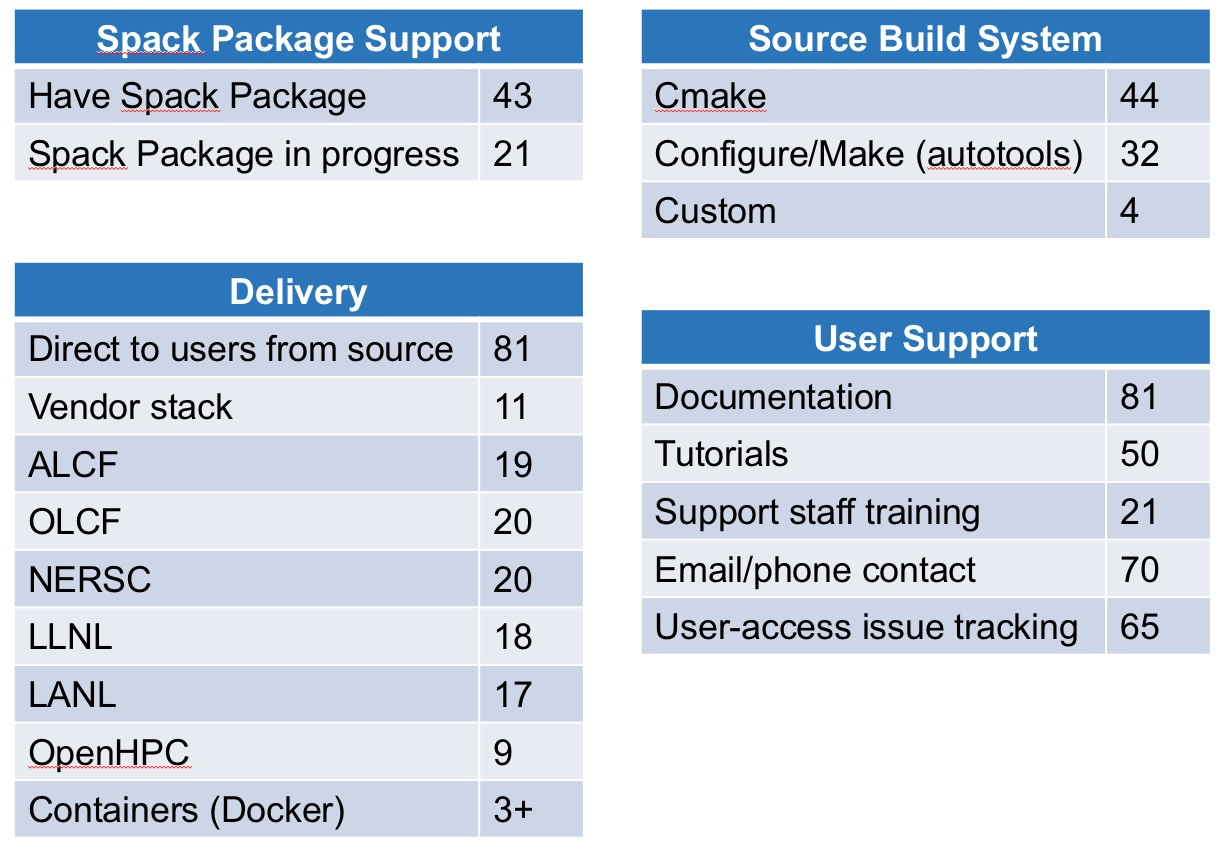
\includegraphics[width=0.7\textwidth]{ProductsOverview}

		\caption{\label{fig:productsoverview}{\small{The 33 ECP ST Projects contribute to 70 user-facing software product suites.   ECP ST products are delivered to users via many mechanisms. Provides experience we can leverage across projects.  Building via Spack is required for participating in ECP ST releases: 50 of the 70 ST product suites are available in the Extreme-scale Scientific Software Stack (E4S) V1.0, release in November 2019.}}}
	\end{center}
\end{figure}

\subsection{ECP ST Products}\label{subsect:products}
 ECP ST efforts contribute to 91 software products in five technical areas (Table~\ref{table:wbs}). 34 of the 91 products are broadly used in the HPC community and require substantial investment and transformation in preparation for Exascale architectures.  An additional 25 are important to some existing applications and typically represent new capabilities that enable new usage models for realizing the potential that Exascale platforms promise.  The remaining products are in early development phases, addressing emerging challenges and opportunities that Exascale platforms present.

\begin{table}
	\begin{tabular}{|l|l|l|}\hline
		\rowcolor{LightCyan}
		\textbf{Product} & \textbf{Website} & \textbf{Deployment Scope}\\\hline
		GASNet-EX & \url{http://gasnet.lbl.gov} & Broad\\\hline
		Kokkos & \url{https://github.com/kokkos} & Broad\\\hline
		MPICH & \url{http://www.mpich.org} & Broad\\\hline
		OpenMPI & \url{https://www.open-mpi.org} & Broad\\\hline
		RAJA & \url{https://github.com/LLNL/RAJA} & Broad\\\hline
		ROSE & \url{https://github.com/rose-compiler} & Broad\\\hline

		CHAI & \url{https://github.com/LLNL/CHAI} & Moderate\\\hline
		Global Arrays & \url{http://hpc.pnl.gov/globalarrays} & Moderate\\\hline
		Legion & \url{http://legion.stanford.edu} & Moderate\\\hline
		LLVM OpenMP compiler & \url{https://github.com/SOLLVE} & Moderate\\\hline
		OpenMP V \& V Suite & \url{https://bitbucket.org/crpl_cisc/sollve_vv/src} & Moderate \\\hline
		Qthreads & \url{https://github.com/Qthreads} & Moderate\\\hline
		Umpire & \url{https://github.com/LLNL/Umpire} & Moderate\\\hline
		UPC++ & \url{http://upcxx.lbl.gov} & Moderate\\\hline
		UMap & \url{https://github.com/LLNL/umap} & Moderate\\\hline

		BOLT & \url{https://github.com/pmodels/bolt} & Experimental\\\hline
		Argobots & \url{https://github.com/pmodels/argobots} & Experimental\\\hline
		Intel GEOPM & \url{https://geopm.github.io} & Experimental\\\hline
		PaRSEC & \url{http://icl.utk.edu/parsec} & Experimental\\\hline
		AML & \url{https://xgitlab.cels.anl.gov/argo/aml} & Experimental\\\hline
		PowerSlurm & \url{https://github.com/tpatki/power-slurm} & Experimental\\\hline
	\end{tabular}
\caption{\label{table:pmr-products} Programming Models and Runtimes Products (18 total).}
\end{table}

\begin{table}
	\begin{tabular}{|l|l|l|}\hline
		\rowcolor{LightCyan}
		\textbf{Product} & \textbf{Website} & \textbf{Deployment Scope}\\\hline

		Caliper & \url{https://github.com/llnl/caliper} & Broad\\\hline
		Dyninst Binary Tools Suite & \url{http://www.paradyn.org} & Broad\\\hline
		HPCToolkit & \url{http://hpctoolkit.org} & Broad\\\hline
		LLVM & \url{http://llvm.org/} & Broad\\\hline
		PAPI & \url{http://icl.utk.edu/exa-papi} & Broad\\\hline
		SCR & \url{https://github.com/llnl/scr} & Broad\\\hline
	    STAT & \url{https://github.com/LLNL/STAT} & Broad\\\hline
		Tau & \url{http://www.cs.uoregon.edu/research/tau} & Broad\\\hline

		mpiFileUtils & \url{https://github.com/hpc/mpifileutils} & Moderate\\\hline
		openarc & \url{https://ft.ornl.gov/research/openarc} & Moderate\\\hline
		Papyrus & \url{https://csmd.ornl.gov/project/papyrus} & Moderate\\\hline
		Program DB Toolkit (PDT) & \url{https://www.cs.uoregon.edu/research/pdt} & Moderate\\\hline
	    PRUNERS Toolset & \url{https://github.com/PRUNERS/PRUNERS-Toolset} & Moderate\\\hline
		TriBITS & \url{https://tribits.org} & Moderate\\\hline

		CHiLL Compiler & & Experimental\\\hline
		Exascale Code Gen Toolkit & & Experimental\\\hline
		Gotcha & \url{http://github.com/llnl/gotcha} & Experimental\\\hline
		Kitsune & \url{https://github.com/lanl/kitsune} & Experimental\\\hline
		QUO & \url{https://github.com/lanl/libquo} & Experimental\\\hline
		SICM & & Experimental \\\hline
		SuRF  & & Experimental\\\hline
\end{tabular}
\caption{\label{table:tools-products} Development Tools Products (21 total).}
\end{table}



\begin{table}
\begin{tabular}{|l|l|l|}\hline
		\rowcolor{LightCyan}
	\textbf{Product} & \textbf{Website} & \textbf{Deployment Scope}\\\hline
	hypre & \url{http://www.llnl.gov/casc/hypre} & Broad\\\hline
	Kokkoskernels & \url{https://github.com/kokkos/kokkos-kernels} & Broad\\\hline
	MFEM & \url{http://mfem.org/} & Broad\\\hline
	PETSc/TAO & \url{http://www.mcs.anl.gov/petsc} & Broad\\\hline
	SLATE & \url{http://icl.utk.edu/slate} & Broad\\\hline
	SUNDIALS & \url{https://computation.llnl.gov/projects/sundials} & Broad\\\hline
	SuperLU & \url{https://portal.nersc.gov/project/sparse/superlu} & Broad\\\hline
	Trilinos & \url{https://github.com/trilinos/Trilinos} & Broad\\\hline

	DTK & \url{https://github.com/ORNL-CEES/DataTransferKit} & Moderate\\\hline
	FleCSI & \url{http://www.flecsi.org} & Moderate\\\hline
	MAGMA-sparse & \url{https://bitbucket.org/icl/magma} & Moderate\\\hline
	STRUMPACK & \url{http://portal.nersc.gov/project/sparse/strumpack} & Moderate\\\hline
	xSDK & \url{https://xsdk.info} & Moderate\\\hline

	FFTX & \url{https://github.com/spiralgen/fftx} & Experimental\\\hline
	ForTrilinos & \url{https://trilinos.github.io/ForTrilinos} & Experimental\\\hline
	libEnsemble & \url{https://github.com/Libensemble/libensemble} & Experimental\\\hline
	Tasmanian & \url{http://tasmanian.ornl.gov} & Experimental\\\hline
\end{tabular}
\caption{\label{table:math-products} Mathematical Libraries Products (16 total).}
\end{table}


\begin{table}
\begin{tabular}{|l|l|l|}\hline
		\rowcolor{LightCyan}
	\textbf{Product} & \textbf{Website} & \textbf{Deployment Scope}\\\hline
	Catalyst (ALPINE) & \url{https://www.paraview.org/in-situ} & Broad\\\hline
	Darshan & \url{http://www.mcs.anl.gov/research/projects/darshan} & Broad\\\hline
	HDF5 & \url{https://www.hdfgroup.org/downloads} & Broad\\\hline
	IOSS & \url{https://github.com/gsjaardema/seacas} & Broad\\\hline
	Parallel netCDF & \url{http://cucis.ece.northwestern.edu/projects/PnetCDF} & Broad\\\hline
	ParaView (ALPINE) & \url{https://www.paraview.org} & Broad\\\hline
	ROMIO & \url{http://www.mcs.anl.gov/projects/romio} & Broad\\\hline
	VeloC & \url{https://veloc.readthedocs.io} & Broad\\\hline
	VeloC & \url{https://xgitlab.cels.anl.gov/ecp-veloc} & Broad\\\hline
	VisIt (ALPINE) & \url{https://wci.llnl.gov/simulation/computer-codes/visit} & Broad\\\hline
	VTK-m & \url{http://m.vtk.org} & Broad\\\hline
	
	ADIOS & \url{https://github.com/ornladios/ADIOS2} & Moderate\\\hline
	ASCENT (ALPINE) & \url{https://github.com/Alpine-DAV/ascent} & Moderate\\\hline
	In Situ Algorithms (ALPINE) & \url{https://github.com/Alpine-DAV/algorithms} & Moderate\\\hline
	Cinema & \url{https://github.com/cinemascience} & Moderate\\\hline
	zfp & \url{https://github.com/LLNL/zfp} & Moderate\\\hline
	
	C2C &  & Experimental\\\hline
	FAODEL & \url{https://github.com/faodel/faodel} & Experimental\\\hline
	GUFI & \url{https://github.com/mar-file-system/GUFI} & Experimental\\\hline
	HXHIM & \url{http://github.com/hpc/hxhim.git} & Experimental\\\hline
	MarFS & \url{https://github.com/mar-file-system/marfs} & Experimental\\\hline
	Mercury & \url{http://www.mcs.anl.gov/research/projects/mochi} & Experimental\\\hline
	ROVER &  & Experimental\\\hline
	Siboka &  & Experimental\\\hline
	SZ & \url{https://github.com/disheng222/SZ} & Experimental\\\hline
	TuckerMPI &  & Experimental\\\hline
	UnifyCR & \url{https://github.com/LLNL/UnifyCR} & Experimental\\\hline
\end{tabular}
\caption{\label{table:vizdata-products} Visualization and Data Products (26 total).}
\end{table}



\begin{table}
\begin{tabular}{|l|l|l|}\hline
		\rowcolor{LightCyan}
	\textbf{Product} & \textbf{Website} & \textbf{Deployment Scope}\\\hline
	Flang/LLVM & Fortran compiler \url{http://www.flang-compiler.org} & Broad\\\hline
	Spack & \url{https://github.com/spack/spack} & Broad\\\hline

	Flux &  \url{http://flux-framework.org} & Moderate\\\hline
	BEE & & Experimental\\\hline
	FSEFI & & Experimental\\\hline
	Sonar & & Experimental\\\hline
	Secure JupyterHub & & Experimental\\\hline
	Kitten Lightweight Kernel & \url{https://github.com/HobbesOSR/kitten} & Experimental \\\hline
	NRM & \url{https://xgitlab.cels.anl.gov/argo/nrm} & Experimental\\\hline
\end{tabular}
\caption{\label{table:eco-products} Software Delivery and Ecosystems Products (12 total).}
\end{table}

\subsection{Standards Committees}
An important activity for ECP ST staff is participation in standards efforts.  In many instances, our software will not be sustainable if it is not tightly connected to a standard.  At the same time, any standard has to take into account the emerging requirements that Exascale platforms need in order to achieve performance and portability.  Figure~\ref{fig:standards} summarized ECP ST staff involvement in the major standards efforts that impact ECP.

ECP ST staff are heavily involved in MPI and OpenMP standards efforts.  ECP ST staff hold several key leadership positions and have heavy involvement in all aspects. ECP ST staff also play a critical role in C++ standards efforts.  While DOE staff have only recently engaged in C++ standards, our efforts are essential to  getting HPC requirements considered, especially by contributing working code that demonstrates requirements and design. ECP ST sponsors the newest open source Fortran compiler Flang~\ref{subsubsect:flang}, a front end for LLVM.  This compiler is a rapidly emerging and essential part of the HPC ecosystem.  In particular, while ARM processors are not explicitly part of the pre-Exascale ecosystem, they are emerging as a strong contender in the future.  Flang is \textit{the} Fortran compiler for ARM-based systems.  ECP ST involvement in other committees, including the \textit{de facto} also provide valuable leverage and improved uniformity for HPC software.  Lastly, we mention the Visualization Toolkit (VTK) Architecture Review Board (ARB).  While this is only a single instance, we intend to explore the ARB model as part of our SDK efforts.
\begin{figure}[htb]
	\begin{center}
		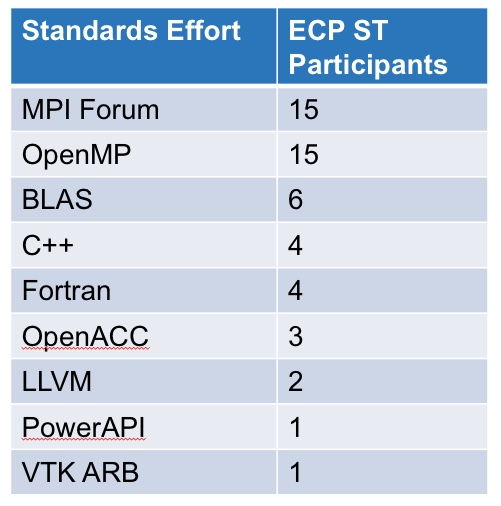
\includegraphics[width=0.5\textwidth]{StandardsInvolvement}
		
		\caption{\label{fig:standards} ECP ST staff are involved in a variety of official and \textit{de facto} standards committees.  Involvement in standards efforts is essential to assuring the sustainability of our products and to assure that emerging Exascale requirements are addressed by these standards.}
	\end{center}
\end{figure}

\subsection{Contributions to External Software Products}\label{subsection:external-contributions}
While much of ECP ST efforts and focus are on the product that we develop and support, it is important to note that some of our important work, and certainly some of our most sustainable and highly leveraged work, is done by providing requirements, analysis, design and prototype capabilities for vendor and other third party software.  Many software studies have shown that 70 to 80\% of the cost of a successful software product goes into post-delivery maintenance. Our effort summarized in Table~\ref{table:externalproducts} expressly eliminate this large cost for DOE because the product is developed and supported outside of DOE.


\begin{table}
	\begin{tabular}{|L{1.5in}|L{4in}|}\hline
			\rowcolor{LightCyan}
			Product & Contribution\\\hline
			Kokkos and RAJA & ECP efforts to provide portable on-node parallel programming and execution environments have led to new features in C++ standards \\\hline
			MPI Forum & ECP ST staff maintain several chapters of the MPI Forum, effort that require a constant involvement with the other authors, as well as participation to the online discussions related to the chapter and regular attendance of the MPI Forum face-to-face activities.\\\hline
			Flang & ECP funds development of the new open source Fortran compiler front end called Flang. Flang provides Fortran language support for LLVM backends, in a similar way as Clang provides support for C and C++.\\\hline 
			All \tools work & Starting in FY20, our \tools\ efforts are organized around delivering capabilities into the LLVM ecosystem.  \\\hline
			SWIG (www.swig.org) & The ECP ST ForTrilinos efforts contributes the capability to generate automatic Fortran bindings from C++ code.\\\hline
			TotalView debugger & ECP ST staff are engaged in co-design of OMPD, the new debugging interface for OpenMP programs, along with RogueWave engineers. This effort helps RogueWave improve their main debugging product, TotalView, by making it aware and compatible with recent advances in OpenMP debugging.\\\hline
			LLVM &  An ECP ST staff member is co-leading design discussions around the parallel IR and loop-optimization infrastructure.\\\hline
			SLATE & ECP ST math libraries efforts inform the design, implementation, and optimization of dense numerical linear algebra routines on most vendor platforms\\\hline
			Cray MPICH MPI-IO & As part of the ExaHDF5 ECP project, the ALCF worked with Cray MPI-IO developers to merge the upstream ROMIO code into the downstream proprietary Cray MPICH MPI-IO, leveraging Cray’s extensive suite of IO performance tests and further tuning the algorithm.  Cray is currently targeting its deployment in an experimental release.\\\hline
			OpenHPC & An ECP ST staff member serves on the OpenHPC Technical Steering Committee as a Component Development representative.\\\hline
		\end{tabular}
		\caption{\label{table:externalproducts} External products to which ECP ST activities contribute.  Participation in requirements, analysis, design and prototyping activities for third-party products is some of the most effective software work we can do.}
	\end{table}



%%---------------------------------------------------------------------------%%
%\vspace{3in}
\clearpage
%\newpage
\section{ECP ST Project Summaries}\label{sect:project-summaries}

This section of the ECP ST Capabilities Assessment Report provides two-page summaries of each funded project.  The text provides a project overview and summarizes the key challenges, solution strategy, recent progress and next steps for the project.
\newpage
\subsection{\pmr}
This section present projects in \pmr.
\newpage

\subsubsection{\pmr\ Software Development Kits} 

\paragraph{Overview} 
The \pmr\ SDK effort is focused on identifying meaningful aggregations of products in this technical area.  SDK efforts are in the early stages of planning and execution.  Most of the work on SDKs has been driven from the \ecosystem\ technical area.  A description of the SDK effort can be found in Section~\ref{subsubsect:ecosystem-sdk}.

\newpage
\subsubsection{LANL ATDM Programming Models and Runtimes}


\paragraph{Overview} 
%\textit{Provide an overview of your project.  You might find that the introductory text from your Fall 2017 Project Summary \url{https://confluence.exascaleproject.org/display/1ST/Fall+2017+ECP+ST+Project+Summaries} useful as a starting draft.}

The LANL ATDM PMR effort is focusing on the development and use of advanced programming models for Advanced Technology Development and Mitigation use-cases. Our current focus is on research and development of new programming model capabilities in the Legion data-centric programming system. Legion provides unique capabilities that align well with our focus on the development of tools and technologies that enables a separation of concerns of computational physicists and computer scientists. Within the ATDM PMR effort we have focused on the development of significant new capabilities within the Legion runtime that are specifically required to support LANL's ATDM applications. Another key component of our work is the co-design and integration of advanced programming model research and development within FleCSI, a Flexible Computational Science Infrastructure. 

A major benefit to the broader ECP community is the development of new features in the Legion programming system which are available as free open-source software \url{https://gitlab.com/StanfordLegion/legion}. 


\paragraph{Key  Challenges} \leavevmode \\
%\textit{Describe what is hard to do, why it is challenging.}

\textbf{Legion.}

Applications will face significant challenges in realizing sustained performance on next-generation systems. Increasing system complexity coupled with increasing scale will require significant changes to our current programming model approaches. This is of particular importance for large-scale multi-physics applications where the application itself is often highly dynamic and can exhibit high variability in resource utilization and system bottlenecks depending on what physics are currently in use (or emphasized). Our goal in the LANL ATDM PMR project is to support these highly dynamic applications on Exascale systems, providing improvements in productivity, long-term maintainability, and performance portability of our next-generation applications. 


\textbf{FleCSI Legion integration.}
FleCSI is a Flexible Computational Science Infrastructure whose goal is to provide a common framework for application development for LANL's next-generation codes. FleCSI is required to support a variety of different distributed data structures and computation on these data structures including structured and unstructured mesh as well as mesh-free methods. Our work in the LANL ATDM PMR project is focused on co-designing the FleCSI data and execution model with the Legion programming model to ensure the latest advancements in the programming model and runtimes research community are represented in our computational infrastructure. A significant challenge in our work is the additional constraint that FleCSI must also support other runtime systems such as MPI. Given this constraint, we have chosen an approach that ensures functional correctness across both runtimes but that also leverages and benefits from capabilities in Legion that are not directly supported in MPI (such as task-based parallelism as a first-class construct). 

\paragraph{Solution Strategy} \leavevmode \\
 
%\textit{Describe your basic strategy for addressing the challenges.}

\textbf{Legion.}

In funded collaboration with NVIDIA, LANL and NVIDIA are developing new features in Legion to support our applications. Necessary features are identified through direct engagement with application developers and through rapid development, evaluation, and refactoring within the team. Major features include Dynamic Control Replication for improved scalability and productivity as well as Fortran interoperability for Legion based applications. 


\textbf{FleCSI Legion integration.}
LANL staff work on co-design and integration of the Legion programming system into the FleCSI framework. We have regular milestones that align well with application needs and the development of new features within Legion. 

\begin{figure}[htb]
        \centering
        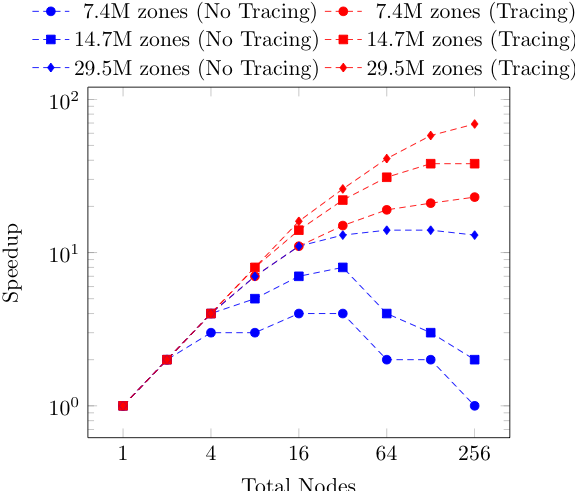
\includegraphics[width=4in]{projects/2.3.1-PMR/2.3.1.02-LANL-ATDM-PMR/tracing-performance}
        \caption{\label{fig:tracing-performance}\textbf{New Legion features such as dynamic tracing significantly improves strong scaling in unstructured mesh computations.}}
\end{figure}




\paragraph{Recent Progress} \leavevmode \\

%\textit{Describe what you have done recently.  It would be good to have some kind of figure or diagram in this section.}


\textbf{Legion.} 
One of the strengths of Legion is that it executes asynchronous tasks as if they were executed in the sequence they occur in the program. This provides the programmer with a mental model of the computation that is easy to reason about. However, the top-level task in this tree-of-tasks model can often become a sequential bottleneck, as it is responsible for the initial distribution of many subtasks across large machines. In earlier work NVIDIA developed the initial implementation of control replication, which allows the programmer to write tasks with sequential semantics that can be  transparently replicated many times, as directed by the Legion mapper interface, and run in a scalable manner across many nodes.
Dynamic control replication is an important capability for LANL's ATDM effort, allowing our application teams to write applications with apparently sequential semantics while enabling scalability to Exascale architectures. This approach will improve understandability of application code, productivity, and composability of software and ease the burden of optimization and porting to new architectures. 


\textbf{FleCSI Legion Integration.} A key component of LANL's Advanced Technology  Development and Mitigation effort is the development of a flexible computational science infrastructure (FleCSI) to support a breadth of application use cases for our Next Generation Code. FleCSI has been co-designed with the Legion programing system in order to enable our Next Generation Code to be performance portable and scalable to future Exascale systems. Legion provides the underlying distributed and node-level runtime environment required for FleCSI to leverage task and data parallelism, data dependent execution, and runtime analysis of task dependencies to expose parallelism that would be tedious and error prone to expose at the application or middleware level. We completed an evaluation of the initial implementation of FleCSI on Legion using the FleCSALE hydrodynamics application. 



\paragraph{Next Steps}  \leavevmode \\


\textbf{FleCSI.} Focus on performance and scalability enhancements of the Dynamic Control Replication and other new Legion features. 

\textbf{FleCSI Legion Integration.} Demonstrate the integration of Dynamic Control Replication and other new Legion features within FleCSI. Our goal is to demonstrate a multi-scale application on the Advanced Technology System, Sierra using our latest advances in the Legion and FleCSI systems. 


\newpage
\subsubsection{\stid{1.0} LLNL ATDM Programming Models and Runtimes}


\paragraph{Overview} 
%\textit{Provide an overview of your project.  You might find that the introductory text from your Fall 2017 Project Summary \url{https://confluence.exascaleproject.org/display/1ST/Fall+2017+ECP+ST+Project+Summaries} useful as a starting draft.}
This project covers two main thrusts in programming models standards and 
runtimes for exascale supercomputing systems. The first thrust is 
programming models standards work in MPI and OpenMP. 

The Message Passing Interface Standard (MPI) is a message passing library standard based on the consensus of the MPI Forum, which has over 40 participating organizations, including vendors, researchers, software library developers, and users. The goal of the Message Passing Interface is to establish a portable, efficient, and flexible standard for message passing that will be widely used for writing message passing programs. As such, MPI is the first standardized, vendor independent, message passing library. The advantages of developing message passing software using MPI closely match the design goals of portability, efficiency, and flexibility. MPI is not an IEEE or ISO standard, but has in fact, become the ``industry standard'' for writing message passing programs on HPC platforms.

OpenMP (Open Multi-Processing) is an application programming interface (API) that supports multi-platform shared memory multiprocessing programming in C, C++, and Fortran, on most HPC platforms. To enable portable tools for performance analysis and debugging of OpenMP programs, the OpenMP Language Committee is defining application programming interfaces for tools; these interfaces are expected to be part of the OpenMP standard and supported by all OpenMP compliant implementations. There are two parts to the proposed interfaces: OMPT (a first-party API for performance tools), and OMPD (a shared-library plugin for debuggers that enables a debugger to inspect and control execution of an OpenMP program).

The other main thrust area for LLNL is the ROSE project’s work in support of 
ATDM Exascale application efforts.  
ROSE is an open source compiler infrastructure to build source-to-source program transformation and analysis tools for large-scale Fortran 77/95/2003, C, C++, OpenMP, and UPC applications. The intended users of ROSE could be either experienced compiler researchers or library and tool developers who may have minimal compiler experience. ROSE is particularly well suited for building custom tools for static analysis, program optimization, arbitrary program transformation, domain-specific optimizations, complex loop optimizations, performance analysis, and cyber-security.



\paragraph{Key  Challenges} \leavevmode \\
%\textit{Describe what is hard to do, why it is challenging.}

\textbf{ROSE.}
We will develop advanced program 
transformation and analysis to improve correctness and performance of 
RAJA codes. The research results will be communicated to RAJA maintainers to 
improve the RAJA portable programming layer. Both of these LLNL efforts 
in this area  are crucial for ECP and ASC applications to achieve portable 
performance on upcoming Exascale systems.

\textbf{MPI.}
For MPI, we focus on 
interfaces for supporting tools, including MPI\_T and MPIR, and for fault
tolerance, including Reinit. Tools for MPI are critical to ensure that
applications achieve high communication performance, and understanding
and designing fault tolerance interfaces are important for large scale
jobs on faulty systems.
The participants will follow development across the standard in
addition to the tools and fault tolerance areas. 

\textbf{OpenMP.} 
In OpenMP, our focus is on the tools interfaces 
OMPT and OMPD.  Tools are critical for application developers to understand
the correctness and performance of their codes when using OpenMP.
We will participate and monitor developments in 
all parts the standard in addition to our focus areas. 

\paragraph{Solution Strategy} \leavevmode \\
 
%\textit{Describe your basic strategy for addressing the challenges.}

\textbf{ROSE.}
The team is working to support advanced loop transformations on RAJA
code; finding loops susceptible to data races in ASC applications;
and performing performance analysis of RAJA code. ROSE improvements
will be released as open source at \url{https://github.com/rose-compiler/rose
}.

\textbf{MPI.}
LLNL staff regularly participate in regular calls and discussions for the Tools Working Group, Fault Tolerance Working Group, Sessions Working Group and attend Forum meetings that occur during the quarter.

\textbf{OpenMP.} Regularly participate in weekly OpenMP language committee calls, participate in biweekly calls of the OpenMP tools WG, email discussions on OpenMP tools interfaces (OMPD and OMPT).

\begin{figure}[htb]
        \centering
        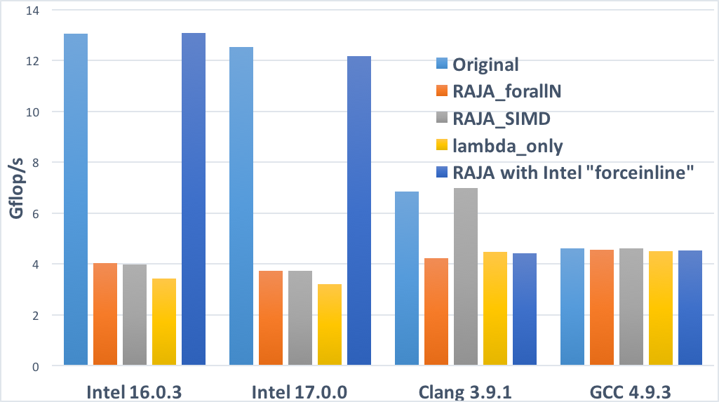
\includegraphics[width=4in]{projects/2.3.1-PMR/2.3.1.03-LLNL-ATDM-PMR/ROSE-raja}
        \caption{\label{fig:rose-raja}\textbf{Work by ROSE team shows
performance gap analysis for RAJA with different compilers.}}
\end{figure}




\paragraph{Recent Progress} \leavevmode \\

%\textit{Describe what you have done recently.  It would be good to have some kind of figure or diagram in this section.}


\textbf{ROSE.} The team continued to improve ROSE's C++11 support 
and the ROSE-based 
tool, rajaChecker. With bug fixes to ROSE, rajaChecker can process 
1650 files in an ASC application without errors, compared to the original 
1405 files.  We also added new features into rajaChecker, such as recognizing 
user-defined RAJA wrappers, MIN/MAX macros, indirect loop index variables, 
etc.  The latest test shows that rajaChecker finds 87 loops in an 
ASC application matching the data race pattern users requested, compared 
to the original 20.



\textbf{MPI.} The MPI participants participated in the design of new 
approaches to incorporate fault tolerance in the MPI Standard, including 
standardizing primitives to support fundamental fault-tolerance methods.  
They also worked on the MPI\_T\_Events interface for tools.
The MPI participants attended the MPI Forum meeting in Portland in 
February and proposed new approaches to incorporate fault tolerance in the 
MPI Standard, including standardizing primitives to support fundamental 
fault-tolerance methods.

\textbf{OpenMP.} In OpenMP, the project members worked with the Tools 
subcommittee to prepare and enact several tickets to improve OMPT 
and OMPD specifications.  The project members attended the OpenMP 
face-to-face meeting in Austin and worked with the Tools subcommittee 
to prepare and enact several tickets to improve OMPT and OMPD 
specifications.


\paragraph{Next Steps}  \leavevmode \\


\textbf{ROSE.} Continue to improve ROSE support for RAJA and ASC applications.

\textbf{MPI.} Continue to participate in MPI Forum on fault tolerance and
tools.

\textbf{OpenMP.} Continue to participate in OpenMP Standards Committee
on tools and debuggers.

\newpage
\subsubsection{SNL ATDM Programming Models: Kokkos} 

\paragraph{Overview} 
Kokkos provides a C++ Parallel Programming Model for Performance Portability. 
It is implemented as a C++ abstraction layer over existing parallel programming models such as OpenMP, CUDA and C++ std::threads. 
Application and library developers can implement their code using Kokkos, 
which will map their parallel algorithms onto the underlying execution mechanism. 
Codes written in that manner can then be compiled to run on each current HPC platform, including CPU and GPU based systems.
Furthermore, new types of architectures generally need only be added to Kokkos, while no changes are necessary to end applications - even if the new architecture requires its own custom programming mechanism. 

\paragraph{Key  Challenges}
Teams of scientists, engineers, and mathematicians apply their specific expertise to develop application software 
to solve problems from their specialized domains. 
The largest and most complex of these require the use of High Performance Computing (HPC). 
For more than two decades, HPC applications used parallel computing on a network of compute-nodes 
consisting of a computer chip with either a single core or very few processing cores 
and memory dedicated to each core. 
However, the “many-core revolution,” which has slowly arisen in the last five years, 
has dramatically changed the nature of HPC because processors in modern compute-nodes 
have many cores that must share the compute-node’s memory.

The many-core revolution in computing is characterized by: 
(1) a steady increase in the number of cores within individual computer chips; 
(2) a corresponding decrease in the amount of memory per core that must be shared by the cores of a chip, and, 
(3), the diversity of computer chip architectures. 
This diversity is highly disruptive because each architecture imposes different complex 
and sometimes conflicting requirements on software to perform well on an architecture. 
Application software development teams are confronted with the dual challenges of: 
(1) inventing new parallel algorithms for many-core chips, 
(2) learning the different programming mechanisms of each architecture, and
(2), creating and maintaining separate versions of their software specialized for each architecture. 
These tasks may involve considerable overhead for organizations in terms of time and cost. 
Adapting application software to changing HPC requirements is already becoming a large expense for 
HPC users and can be expected to grow as the diversity of HPC architectures continues to rise.
An alternative, however, is creating software that is performance portable across current and future architectures. 

A key issue for achieving performance portability is, that one does not only need to address parallel execution but also data management. 
This includes the handling of memory hierarchies consisting of resources such as HBM, DDR and NVM memory as well as the question of memory layouts, which might need to be different for various architectures. 

\paragraph{Solution Strategy}

The Kokkos project developed a parallel programming model with flexible enough semantics that it can be mapped on a diverse set of HPC architectures including current multi-core CPUs and massively parallel GPUs. 
The programming model is implemented using C++ template abstractions, which allow a compile time translation to the underlying programming mechanism on each platform, using their respective primary tool chains. 
Compared to approaches which rely on source-to-source translators or special compilers, this way leverages the investment of vendors in their preferred programming mechanism without introducing additional, hard to maintain, tools in the compilation chain. 

\begin{figure}[ht!]
\centering
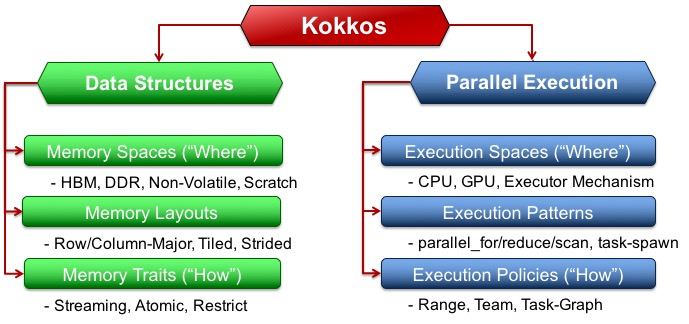
\includegraphics[width=90mm]{projects/2.3.1-PMR/2.3.1.04-SNL-ATDM-PMR/kokkos-abstractions.jpg}
\caption{Kokkos Execution and Memory Abstractions}
\end{figure}

Applications written in Kokkos are leveraging its six core abstractions for parallel execution and data management. 
These abstractions provide the flexibility to allow the mapping of execution and data to the diverse set of architectures. 
As an example the "parallel\_for" Execution Pattern does neither guarantee order of execution nor concurrency of execution. 
That allows Kokkos to use threading, vectorization or even pipelining of operations to parallelize the algorithm. 

The Parallel Execution abstractions are (1) Execution Patterns, (2) Execution Policies, and (3) Execution Spaces. 
{\it Execution Patterns} describe what fundamental parallel algorithm is performed. This includes parallel loops, parallel reductions, and parallel scans as well as task spawn operations. 
{\it Execution Policies} control how the patterns are executed. They for example control the iteration space and whether scheduling is done dynamically or statically.
{\it Execution Spaces} denote different resources to execute on such as GPU or CPU. 

The Memory abstractions are (1) Memory Layout, (2) Memory Traits, and (3) Memory Space). 
{\it Memory Layout} describes the mapping of logical indices to the actual memory address. 
This allows to change the data access pattern in an algorithm without changing the implementation of the algorithm.
{\it Memory Traits} describe access properties, such as whether the user wants to perform atomic accesses, or whether accesses are guaranteed non-aliased. 
{\it Memory Spaces} control where data is allocated. This allows users to access HBM and DDR memory as well as special Scratch Memory. 


As a programming model, Kokkos is highly invasive in any code it is used by. 
Consequently, software quality is a critical concern.
Kokkos addresses this through a comprehensive testing regime, which includes over 250 combinations of compilers, hardware platforms and backends which are run every night. 
These tests cover current production HPC environments as well as prototype environments for future systems. 

Kokkos is available to users under the BSD license, permitting use of Kokkos in other open source codes as well as closed source code. 
It is maintained and developed at {\it https://github.com/kokkos/kokkos}. 

\paragraph{Recent Progress}

Kokkos is now used by a wide number of applications at various institutions. 
This includes multiple DOE laboratories as well as universities and other HPC centers.
At Sandia National Laboratories Kokkos is the primary programming model to address support for GPU based platforms in a performance portable manner, and numerous production level applications are actively porting to using Kokkos. 
The SNL ATDM applications are largely demonstrating performance portability today for a subset of their capabilities and are working towards full fletched support of all HPC platforms. 

Recent advances in Kokkos include support for more portable and performant scatter-add type algorithms, dynamic and static task graph support as well as support for NIVDIA Volta and ARM CPU architectures. 
This enables Kokkos applications to run on the DOE Summit and Sierra machines, which are getting installed now as well as at the upcoming Vanguard ARM based machine to be installed at Sandia in Summer 2018. 
  
\paragraph{Next Steps}

The Kokkos team is working with the Path Forward vendors to enable support for their architectures. 
This notably includes a new backend, called ROCm, for AMD GPUs, which is primarily developed by AMD itself. 
Furthermore, improvements on the dynamic task graph execution on GPUs are planned, in order to reduce the task granularity necessary to make effective use for GPUs. 

%\newpage
%%!TEX root = main.tex

\subsubsection{\stid{1.04} SNL ATDM Programming Models: DARMA} 

\paragraph{Overview} 
DARMA (Distributed, Asynchronous, Resilient Models for Applications) embeds safe and performant asynchronous tasking constructs in C++.
DARMA defines asynchronous semantics for C++, providing a futures-based programming model. 
DARMA, however, provides additional semantics that carry extra safety and performance guarantees,
including race freedom, fully non-blocking execution, and simplified load balancing and communication overlap.
These semantics are implemented as a standards-compliant C++ header library,
embedding asynchronous execution via metaprogramming.

\paragraph{Key Challenges}
Dynamic applications can be characterized by either unknown, imbalanced, or rapidly varying computation loads and communication patterns.
Particle-in-cell, for example, has varying computational load per mesh region. As particles migrate, it also requires dynamic termination detection before entering a field solve phase. 
Overlap detection in contact algorithms rapidly creates load imbalance, which must be mitigated dynamically, in regions where contact occurs. Addressing these algorithmic challenges can involve:
\begin{itemize}
\item Latency-hiding of communication by trying to improve overlap with computation
\item Elastic tasks with built-in data parallelism that can leverage more cores for larger tasks
\item Asynchronous quiescence detection to avoid global synchronizations and minimize communication
\item Semi-static load balancing (globally synchronous) for problems with persistent load imbalance
\item Dynamic load balancing (work stealing) for problems with rapidly varying load imbalance
\end{itemize}
One possible option is for application developers to pursue domain-specific, ad hoc solutions.
Managing things like resource contention between elastic tasks or implementing spanning trees for quiescence are highly non-trivial.
A far more sustainable and productive approach would be providing these execution patterns in a reusable library with implementation complexities hidden behind a productive programming model.
Programming should emphasize problem decomposition, data effect specification for correctness, and domain-specific cost models and heuristics for performance portability.
The key challenges are both defining the programming abstractions to be used at application-level and implementing these dynamic execution constructs at the runtime-level.

\paragraph{Solution Strategy}
Similar to standard futures that create data-flow for C++ datatypes,
DARMA provides asynchronous pointers with well-defined semantics that augment data-flow with non-blocking and race freedom guarantees.
DARMA asynchronous pointers cab define serialization for arbitrary C++ types, enabling load balancing and asynchronous communication overlap.
DARMA asynchronous pointers are intended to express concurrency in a sufficiently general way that multiple runtimes could serve as the backend implementation (Figure~\ref{fig:darmaStack}).
To date, HPX (futures/promises), Charm++ (actor model), and MPI + OpenMP have all been able to provide relatively lightweight implementations despite their obvious design differences.


\begin{figure}
\centering
\includegraphics[width=0.5\textwidth]{projects/2.3.1-PMR/2.3.1.04-SNL-ATDM-PMR/DARMA_Software_Stack.pdf}
\caption{DARMA software stack model showing application-level code implemented with asynchronous programming model (DARMA header library).
Application-level semantics are translated into a task graph specification via metaprogramming in the translation layer. Glue code maps task graph specification to individual runtime libraries. Current backend implementations include std::threads, Charm++, MPI + OpenMP, and HPX.}
\label{fig:darmaStack}
\end{figure}
%\end{minipage}

%\begin{minipage}{0.5\textwidth}
%\begin{figure}
%\includegraphics[width=0.9\textwidth]{DARMA_Software_Stack.pdf}
%\end{figure}
%\end{minipage}

Another general approach consistent with the DARMA model for reducing algorithmic complexity is task \emph{over-decomposition} in the context of shared-memory parallelism.
For example, taking an MPI rank as the fundamental unit, over-decomposition would create many (e.g. 4-16) regions or patches per MPI rank,
rather than a single large patch as would be most common.
Overdecomposition aims to avoid complexities in explicit, application-level load balancing and explicit, application-level communication latency hiding.
When load imbalance occurs, entire tasks can be migrated without requiring re-meshing or updating data structures.
Similarly, communication occurs transparently through task dependencies, naturally pipelining and overlapping communication without requiring explicit Isend/wait constructs.

DARMA allows algorithms to be expressed with flexible granularity, tuning overdecomposition factors to meet either a hardware requirement (e.g. optimal balance of communication overlap and scheduling overhead, task blocking to fit caches) or an algorithmic requirement (e.g. sufficiently fine granularity for load balancing).
Recent DARMA-Kokkos integration now allows over-decomposition on a per-node basis, rather than per-core.
This greatly minimizes task scheduling overheads and can improve communication throughput (surface area-to-volume considerations).
This further improves load balancing flexibility by allowing DARMA to control not only the number of tasks per node but the number of cores allocated to each task.

\paragraph{Recent Progress}
DARMA constructs are being used in the development of ATDM applications, including particle-in-cell (as part of EMPIRE), multiscale physics (in the ATDM tech demonstrator), and contact applications.  MPI interoperability constructs have been defined and recently implemented. DARMA has integrated with Kokkos, providing support for data-parallel tasks.

\paragraph{Next Steps}
The next steps are pursuing both continued adoption in further applications, continued implementation of the programming model with additional backends, and continued improvement of the MPI + OpenMP reference implementation.
For application adoption, a major focus will be using the MPI interoperability constructs to interface Trilinos solvers with DARMA kernels.
Code improvements of the MPI reference implementation will focus on more load balancing heuristics, performance and correctness debugging, and demonstration at increasing scales on capability platforms like Trinity, Cori, and Sierra.
DARMA is also active on the C++ standards committee, particularly for the parallelism technical specification. DARMA-inspired library features are being actively proposed and considered.
%\newpage
%\subsubsection{xGA} 

\paragraph{Overview} 

The xGA project is focused on improving the performance, scalability,
and user productivity of the Global Arrays (GA) library for exascale
systems.  This is essential to the ECP applications that already depend
on GA such as NWChemEx\cite{xGA_NWCHEM}, GAMESS\cite{xGA_GAMESS} and
GridPACK\cite{xGA_GRIDPACK} (used as part of the Stochastic Grid
Dynamics project).  In addition, GA is being considered for use in the
ECP application QMCPACK\cite{xGA_QMCPACK}.

GA supports a shared memory-like programming model on distributed memory
platforms.  This allows users to create distributed multidimensional
arrays that can be accessed from any processor using simple one-sided
put/get/accumulate communication primitives. Data consistency is maintained
using global synchronization mechanisms that flush all outstanding communication
from the system and guarantee that arrays are in a known state.
We are extending the GA library in a number of ways to take advantage of
exascale architecture features including
deep memory hierarchies and accelerators, while continuing to tune and
improve the performance of the GA runtime.

\paragraph{Key  Challenges}

Application codes increasingly need to take advantage of emerging
hardware features to support more sophisticated scientific models. These
hardware features extend the computing model beyond the concept of one compute
thread per communication process as well as extending the memory model beyond
the idea of a single flat view of data. Some of these Exascale platform features
include massively multi-core CPUs, improved network communication speeds, the
availability of GPU accelerators, and deep memory hierarchies. Any one or more
of these capabilities promises to accelerate application codes, so long as these
features are supported by the underlying runtimes and are accessible
through easy-to-use interfaces.

Partitioned Global Address Space (PGAS) models have emerged as a popular
alternative to MPI models for designing scalable applications. These are
typically paired with a one-sided communication model and are particularly
well-suited for applications with irregular access patterns that are not easily
predicted in advance.
%At the same time, MPI remains a ubiquitous communication
%subsystem due to its standardization, high performance, and availability on leading
%platforms.
Though MPI implementations are modernizing with features such as
GPUDirect technology, PGAS models have not maintained similar advances.
Users are requesting that PGAS models provide similar, seamless
features for addressing and communicating with memory that may be located
anywhere within the memory hierarchy, including memory resident on
accelerators. They are also interested in using communication calls from
multiple independent threads within a single traditional communication process.
%Both of these present significant challenges.
The lack of a consensus model for
deep memory hierarchies makes developing a single interface for exploiting these
by GA
%, or any other application for that matter,
extremely difficult.
Supporting multi-threaded applications in a robust and efficient manner is also
likely to require significant software engineering in order to remove locks and
achieve high performance.

\paragraph{Solution Strategy}

The xGA project has three primary thrusts:
\begin{enumerate}
\item \textbf{Thread safety:} GA has not previously provided any thread safety
features or specification.
\item \textbf{Deep memory:} Users should provide hints to allocate GA
memory anywhere within the memory hierarchy, including NVMe and GPUs. 
\item \textbf{Application integration:} Any new feature should directly
benefit one or more ECP applications.
\end{enumerate}

\paragraph{Recent Progress}

\begin{enumerate}
\item \textbf{Thread safety:} GA has not previously provided any thread safety
features or specification. We have recently implemented a preliminary strategy
for thread safety that puts locks on all communication calls. In principle, this
could be fairly efficient, since communications calls are not all occurring at
the same time, but the overhead of creating and destroying the locks themselves
seems to be a severe drag on performance. We are currently reviewing individual
calls to remove global variables where possible with a view to creating
lock-free versions of these calls that can be used by a multi-threaded
application.

\item \textbf{Deep memory:} We have begun looking at developing a strategy for
creating GAs on GPU memory.

\item \textbf{Application integration:} GA is used in three applications
currently supported by ECP. These include NWChemEx (via the TAMMS runtime layer),
Stochastic Grid Optimization (via GridPACK) and GAMESS. We are also in discussions
with QMCPACK application about using GA to support large distributed lookup tables
of spline coefficients. We expect that QMCPACK, as well as potentially NWChemEx,
would benefit from a read-only property that we have been working on within GA.
We are also discussing with NWChemEx how to potentially use thread-safe calls in
GA as well as exploiting the deep memory hierarchy.

\item \textbf{Data layout:} We have developed new options for controlling the
data layout within GAs. The internal routines for accessing both local and
remote data have been completely reorganized to use an iterator model that has
eliminated a lot of redundant code in the current implementation. It has also
allowed us to implement a new 'tiled' array option guarantees that data is laid
out in user-controlled blocks that are contiguous in memory. These layouts match
layouts that are being considered by some of the linear algebra libraries and
provide options for optimizing communication by eliminating strided
communication calls. We have also begun a preliminary implementation of a
sparse data layout designed to support sparse 2D array operations. We have used
this to implement a sparse matrix-vector multiplication operation.

\item \textbf{Improved Performance:} We are continually evaluating and
improving our performance. Figure~\ref{fig:ga_bw} shows how we recently
improved the bandwidth of our strided get operation in our 5.7 release
of the Progress Rank ComEx runtime\cite{xGA_COMEX}.
\end{enumerate}

\begin{figure}[htb]
    \centering
    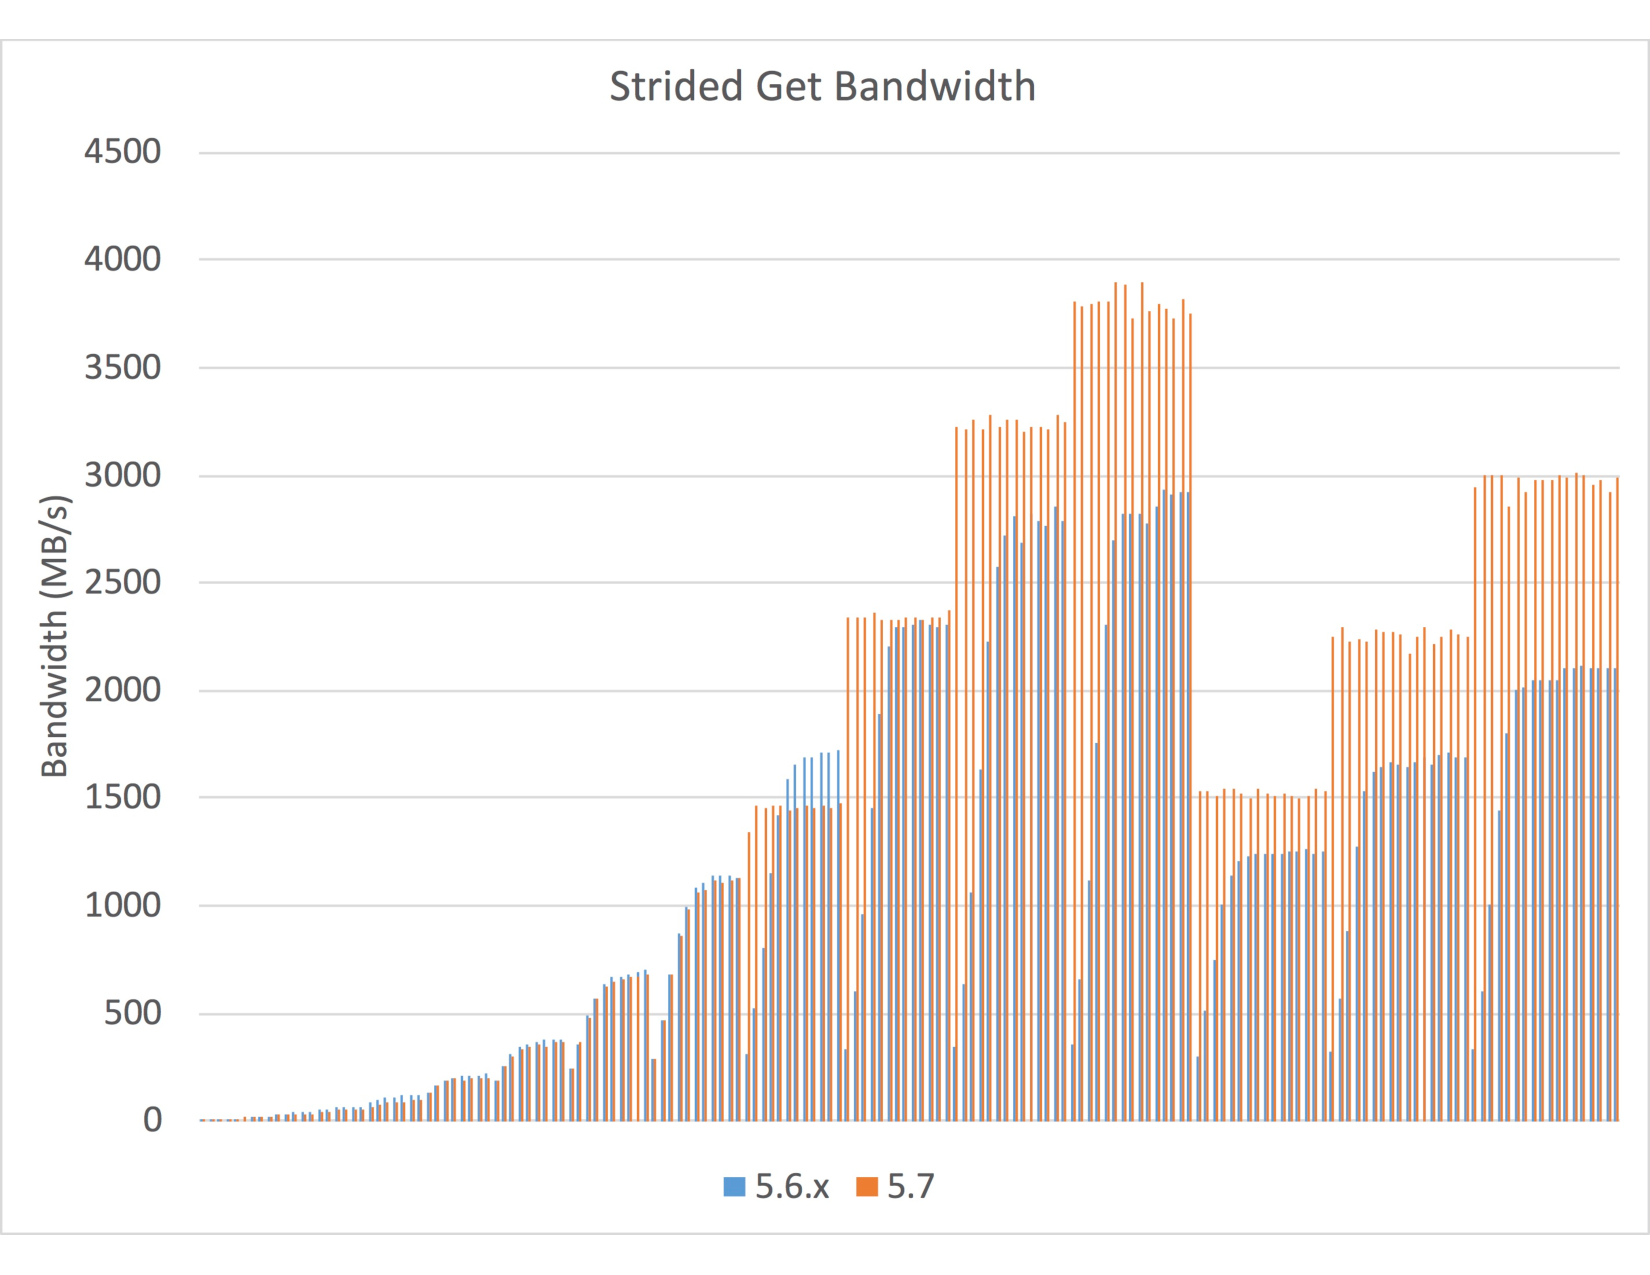
\includegraphics[width=0.7\columnwidth]{projects/2.3.1-PMR/2.3.1.05-Global-Arrays/GA_get_bw}
    \caption{\label{fig:ga_bw}Improved performance of strided get in the 5.7 release series.}
\end{figure}

\paragraph{Next Steps}

Our next steps are:

\begin{enumerate}
\item \textbf{Add hints targeting memory hierarchy allocation:} xGA will
expand its array property types allowing users to specify where memory
should be allocated. We will also continue to refine the read-only property to
include caching of requests so that we can expand the property to handle very
large arrays. Currently, the property is limited to arrays that can be stored on
a single node.
\item \textbf{Improved thread-safe performance:} We will improve our
thread-safe performance by eliminating the use of globally shared variables and
the locks that surround one-sided GA operations. In some cases, it may not be
possible to implement thread-safe solutions without locks with the existing
interface. In these cases, we will look to extending the interface to provide
thread-safe alternatives that will deliver high performance.
\end{enumerate}

\newpage
\subsubsection{\stid{1.06} ISC4MCM (RAJA)} 

\paragraph{Overview.} 
The Integrated Software Components for Managing Computation and Memory 
Interplay at Exascale (ISC4MCM) project is providing software libraries that 
enable application and library developers to meet advanced architecture 
portability challenges. The project goals are to enable writing performance 
portable computational kernels and coordinate complex heterogeneous memory 
resources among components in a large integrated application. These 
libraries enhance developer productivity by insulating them from much of the 
complexity associated with parallel programming model usage and 
system-specific memory concerns.

The software products provided by this project are three complementary and 
interoperable libraries:
\begin{enumerate}
\item {\bf RAJA:} Software abstractions that enable C++ developers to write
  performance portable (i.e., single-source) numerical kernels (loops). 
\item {\bf CHAI:} C++ ``managed array'' abstractions that enable transparent
  and automatic copying of application data to execution memory spaces at run
    time as needed based on RAJA execution contexts.
\item {\bf Umpire:} A portable memory resource management library that provides
  a unified high-level API for resource discovery, memory provisioning,
    allocation, access, operations, and introspection.
\end{enumerate}

Capabilities delivered by these software efforts are needed to manage the
diversity and uncertainty associated with current and future HPC architecture
design and software support. Moving forward, ECP applications and libraries 
need to achieve performance portability: without becoming bound to particular
(potentially-limiting) hardware or software technologies, by insulating 
numerical algorithms from platform-specific data and execution concerns, and 
without major disruption as new machine, programming models, and vendor
software become available.

These libraries in development in this project are currently used in production
ASC applications at Lawrence Livermore National Laboratory (LLNL). They are
also being used or being explored/adopted by several ECP application and
library projects, including: LLNL ATDM application, GEOS (Subsurface), SW4
(EQSIM), MFEM (CEED co-design), and SUNDIALS.

The software projects are highly-leveraged with other efforts. Team members
include: ASC and ATDM application developers, ASD tool developers, university
collaborators, and vendors. This ECP ST project supports outreach to the ECP
community and collaboration with ECP efforts.

\paragraph{Key Challenges.}

The main technical challenge for this project is enabling production
applications to achieve performance portability in an environment of rapidly
changing, disruptive HPC hardware architecture design. Typical large
applications contain $O(10^5) - O(10^6)$ lines of code and $O(10K)$ loop
kernels. The codes must run efficiently on platforms ranging from laptops to
commodity clusters to large HPC platforms. The codes are long-lived and are
used daily for decades, so they must be portable across machine generations.
Also, the codes are under continual development, with a steady stream of new
capabilities added throughout their lifetimes -- continual validation and
verification is essential, which precludes substantial rewrites from scratch.
Lastly, the complex interplay of multiple physics packages and dozens of
libraries makes it so that the data required for the full set of components
needed for a given simulation may not fit into a single system memory space. To
advance scientific computing capabilities, applications must navigate these
constraints while facing substantial hardware architecture disruption along the
road toward Exascale computing platforms. 

While the software provided by this project has a substantial user base at
LLNL, achieving broader adoption in the ECP (projects without LLNL involvement,
in particular) is another challenge. The software efforts are funded almost
entirely by LLNL programs and the majority of their developers work on LLNL
application projects. So resource limitations is a key issue.

\paragraph{Solution Strategy.}

The software libraries in this project focus on encapsulation and 
application-facing APIs to insulate users from the complexity and 
challenges associated with diverse forms of parallelism and heterogeneous 
memory systems. This approach allows users to exploit new capabilities 
with manageable rewriting of their applications.

RAJA provides various C++ abstractions for parallel loop execution. It
supports: various parallel programming model back-ends, such as OpenMP 
(CPU multithreading and target offload), CUDA, Intel Threading Building Blocks,
etc.; loop iteration space and data view constructs to reorder, 
aggregate, tile, and partition loop iterations; complex loop kernel 
transformations for optimization, such as reordering loop nests, fusing 
loops, etc. RAJA also supports portable atomic operations, parallel scans, 
and CPU and GPU shared memory. After loops have been converted to RAJA, 
developers can explore implementation alternatives via RAJA features without 
altering loop kernels at the application level.

CHAI provides C++ ``managed array'' abstractions that automatically copy 
data to execution memory spaces as needed at run time based on RAJA execution 
contexts. Access to array data in loop kernels looks the same as when using
traditional C-style arrays.

Umpire provides a portable API for managing complex memory resources by 
providing uniform access to other libraries and utilities that provide
system-specific capabilities. Umpire decouples resource allocation from 
specific memory spaces, allocators, and operations. The memory introspection 
functionality of Umpire enables applications and libraries to make memory 
usage decisions based on allocation properties (size, location, sharing 
between packages, etc.)

All three software libraries are open source and available on
GitHub~\cite{RAJA-github, CHAI-github, Umpire-github}. There they provide
regular software and documentation releases. Each project has dedicated email
lists, issue tracking, test suites, and automated testing.

\paragraph{Recent Progress}

In FY18, CHAI and Umpire have been released as open source software projects
and they are now developed on GitHub Recent development has focused on 
user documentation and cleaner integration of these two libraries to give 
applications more flexible and easy access to their capabilities.

Many new features have been added to RAJA in FY18 to enable flexible
loop transformations for complex loop kernels via execution policies.
LLNL applications are assessing this new functionality now in a 
"pre-release" version; it will be generally available before the end of FY18.

The RAJA Performance Suite~\cite{RAJAPerf-github} was released and made 
available on Github in January 2018. The Suite is used to assess and track 
performance of RAJA across programming models and diverse loop 
kernels. It is also being used for compiler acceptance testing in the CORAL 
procurement and was prepared for use as a benchmark for the CORAL-2 procurement.

In 2018, the RAJA project expanded its visibility beyond DOE NNSA Labs. 
Recent presentations include a RAJA tutorial at the 2018 ECP Annual Meeting 
and an application use case study the 2018 NVIDIA GPU Tech Conference (GTC). 
Future tutorials are planned at 2018 ATPESC and GTC 2019. Also, a RAJA paper 
and $1/2$-day tutorial proposal were submitted to SC18.

\paragraph{Next Steps}

Our next efforts include:
\begin{enumerate}
\item {\bf Fill RAJA Gaps:} Not all features are available for all programming
  model back-ends; as models mature, such as OpenMP4.5, these gaps will be
    filled.
\item {\bf Expand RAJA User Guide and Tutorial:} Build example codes and user
  documentation for latest RAJA features and prepare for future tutorials
    (ATPESC 2018 and SC18).
\item {\bf Expand RAJA Performance Suite:} Include kernels that exercise more
  application use cases and RAJA features.
\item {\bf Focus RAJA Vendor Interaction:} Work with CORAL vendors to address
  issues as applications port to the Sierra platform at LLNL; establish early
    interactions with CORAL-2 vendors to ensure RAJA will be supported well on
    CORAL-2 systems.
\item {\bf Expand Umpire Capabilities:} Explore potential collaboration with
  relevant ECP efforts, such as SICM project.
\end{enumerate}

\newpage
\subsubsection{\stid{1.07} Exascale MPI} \label{subsubsect:mpich}
\paragraph{Overview}

MPI has been the de facto standard programming model for HPC from the
mid 90's till today, a period where supercomputing performance
increased by six orders of magnitude.  The vast majority of DOE's
parallel scientific applications running on the largest HPC systems
use MPI. These application codes represent billions of dollars of
investment. Therefore, MPI must evolve to run as efficiently as
possible on Exascale systems. Our group at Argonne developed a
high-performance, production-quality MPI implementation, called MPICH.
The focus areas of the Exascale MPI / MPICH project are: (1)
continuous improvement of the performance and capabilities of the
MPICH software to meet the demands of ECP and other broader DOE
applications, (2) coordinate vendor and supercomputing center
interactions to ensure efficient solutions to applications, and (3) be
involved in the MPI forum and standardization efforts to ensure
continuity of the work beyond this project.

MPICH team is involved in the formation of the MPI Forum and have been
deeply involved in defining the MPI standard since 1992. MPICH has
helped prototype and define the majority of the features in the MPI
standard. As such, MPICH has been one of the most influential pieces of
software in accelerating the adoption of the MPI standard by the HPC
community. MPICH has been adopted by leading vendors into their own
derivative implementations. Examples include Intel (for Intel MPI), Cray
(for Cray MPI), IBM (for IBM PE MPI), Mellanox (for MLNX-MPI), Microsoft
(for MS-MPI), and Ohio State University (for MVAPICH). MPICH and its
derivatives are exclusively used in 7 of the top 10 supercomputers in
the world today. MPICH is the recipient of a number of awards including
an R\&D 100 award.

\paragraph{Key Challenges}

While we believe MPI is a viable programming model at Exascale, both
the MPI standard and MPI implementations have to address the
challenges posed by the increased scale, performance characteristics
and evolving architectural features expected in Exascale systems, as
well as the capabilities and requirements of applications targeted at
these systems. The key challenges are:

\begin{enumerate}

\item Interoperability with intranode programming models having a high
  thread count~\cite{Hybrid1, Hybrid2, FT2} (such as OpenMP,
  OpenACC and emerging asynchronous task models);

\item Scalability and performance over complex
  architectures~\cite{Perf1, Perf2, FT2, Perf4} (including high core
  counts, processor heterogeneity and heterogeneous memory);

\item Software overheads that are exacerbated by lightweight cores and
  low-latency networks;

\item Enhanced functionality (extensions to the MPI standard) based on
  experience with applications and high-level libraries/frameworks
  targeted at Exascale; and

\item Topics that become more significant as we move to the next
  generation of HPC architectures: memory usage, power, and
  resilience.

\end{enumerate}

\paragraph{Solution Strategy}

The Exascale MPI project has the following primary technical thrusts:
(1) \textbf{Performance and Scalability} (2) \textbf{Heterogeneity}
(3) \textbf{Topology Awareness} (4) \textbf{Fault Tolerance} and (5)
\textbf{MPI+X Hybrid Programming}.

Our solution strategy started by addressing performance and
scalability aspects in MPICH related to network address
management~\cite{memscal}.  Apart from this, we also looked at
communication strategies which allow the MPI library to be as
lightweight as possible~\cite{ch41, ch42}. Other solutions include
investigation and evaluation of communication relaxation hints,
investigation of optimizations to memory scalability in MPICH and
improvements to MPI RMA operations.

Exascale MPI heterogeneity efforts~\cite{Hetero1, Hetero2, Hetero3}
started with the survey on heterogeneous memory architectures on
upcoming DOE machines and how MPICH can take advantage of
them~\cite{hexe}. The efforts also included the investigation of
utilizing heterogeneous memory inside the MPI implementation and
evaluation of applications~\cite{hetero4}. The heterogeneity efforts
further extended to investigating and developing technologies for GPU
integration for the better support of the coming Exascale
supercomputers.

Exascale MPI topology awareness efforts~\cite{Topo1,Topo2} originated
with the investigation and evaluation of hints based on topology
awareness and optimizations to virtual topology functionality in
MPICH~\cite{topo-io,topo-io2}. The other efforts include investigation
of topology-aware collectives and neighborhood collectives in
MPICH~\cite{coll} and evaluation of the selected ECP applications.

Exascale MPI fault tolerance efforts~\cite{FT1, FT2} started with
support for handling noncatastrophic errors in MPI. The second effort
included defining the scope of errors in MPI, a prerequisite for
user-level failure mitigation (ULFM). Other efforts in this direction
includes standardizing ULFM in MPI and evaluating application
suitability for fault tolerance.

Exascale MPI+X hybrid programming developed firstly with effort in
improving interoperation of MPICH with threads~\cite{interthread}.
Secondly, we developed the work-queue data transfer model for
multithreaded MPI communication~\cite{workq}. We have included support
for interaction of MPICH with user-level thread (ULT)
libraries~\cite{ULT}, primarily targeting Argobots and the BOLT
runtime~\cite{BOLT}.  Other issues that are being looked at include the
investigation and evaluation on interaction between MPI and OpenMP and
the study and evaluation of MPI endpoints.

\paragraph{Recent Progress}

Figure~\ref{fig:fy19} provides the details of major milestones completed
in FY2019. In the first milestone, we studied the performance
of the RMA improvements using the large quantum chemistry application
suite NWChem (version 6.6) with ARMCI-MPI and MPICH on the Cray XC40
supercomputer. The results shown that enabling network hardware atomics
with the info hints fully eliminated the performance bottleneck in the
Density Functional Theory (DFT) module and improved the performance
scalability of NWChem DFT. In the second milestone, we studied the
performance impact of ULFM when there is no failure. A study report has
been submitted on performance analysis of the ULFM prototype. In the
third milestone, we studied the performance of MPI Endpoints. The
results shown significant improvement of using MPI endpoints
prototype---the multithreaded MPI communication reached a message rate
that is close to the case of single-threaded MPI communication. We
concluded that exposing the application level parallelism to the MPI
through the use of endpoints enables effectively scheduling of the
traffic. In such a way, multiple hardware resource can be utilized to
reduce the contention between threads and improve performance.

\begin{figure}[htb]
  \centering
  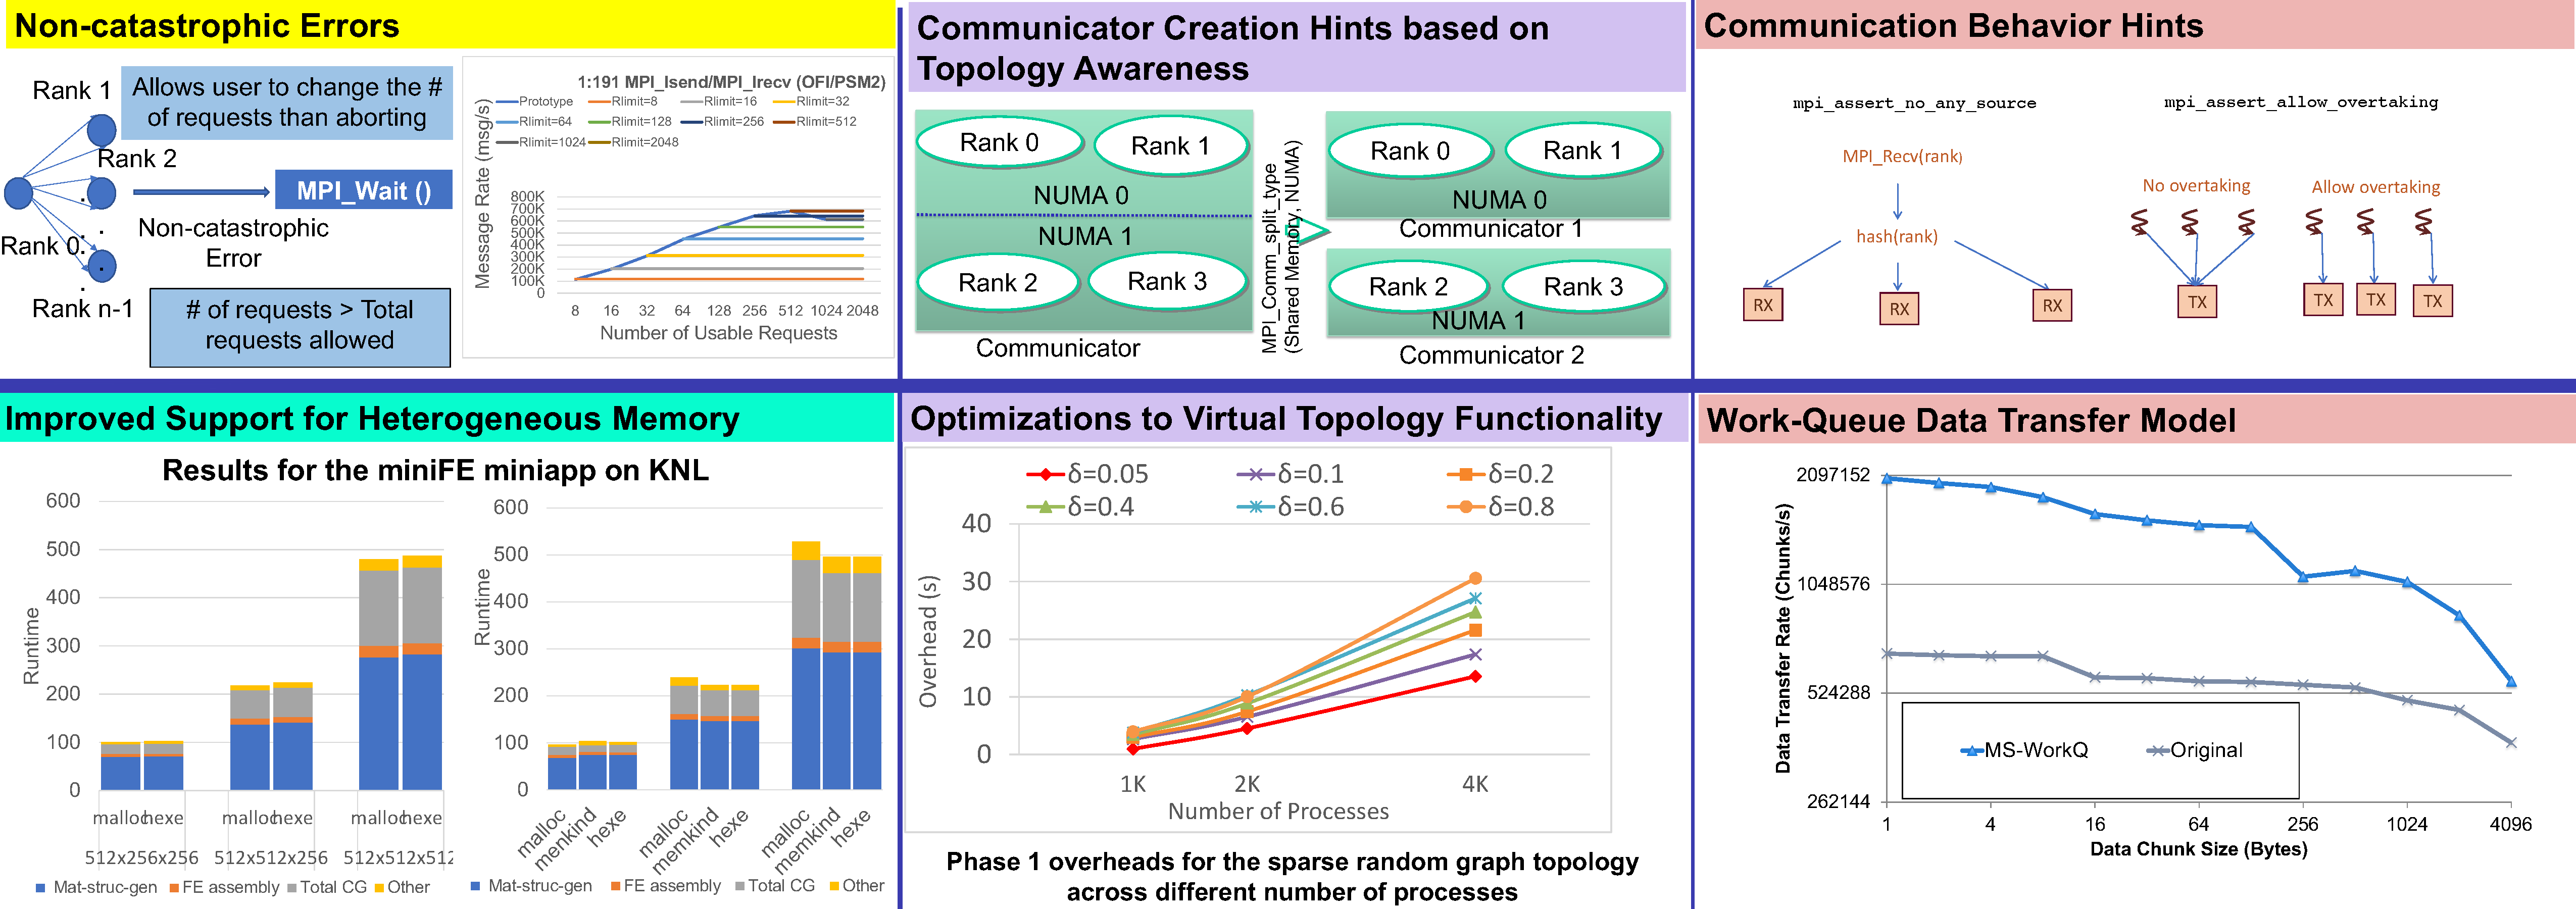
\includegraphics[width=6in]{projects/2.3.1-PMR/2.3.1.07-Exascale-MPI/MPICH-recent-milestones.pdf}
  \caption{\label{fig:fy19}Major MPICH milestones completed in fiscal year 2019}
\end{figure}

In the fourth milestone, we evaluated the benefit of using
topology-aware neighborhood collectives. We used the neighborhood
collective integration in the PETSc scalable linear solvers (KSP)
component for this evaluation. The results did show benefit, but with a
caveat that is the neighborhood collectives incurs significant setup
cost which currently overshadowing the communication benefit. The
addition of ``persistent'' collective operations in MPI-4 will allow us
to remove the per-operation setup cost. In the last milestone, we
performed comprehensive evaluation of the project which included
functional tests and performance tests.  The experiment results using
Nek5000 on OLCF Summit supercomputer shown significant improvements in
performance and scalability due to the techniques developed in this ECP
project.

\paragraph{Next Steps}
A major focus of the ongoing Exascale MPI efforts is MPI+GPU
improvements. This includes improvements for
multiple accelerator nodes and native hardware models, support for
noncontiguous data and software evaluations. Exascale MPI ongoing
efforts also includes a developing a collective selection framework for
improving the performance and scalability of collectives. We are also
making efforts in MPI standardization which includes investigation
application usage of MPI and incorporating those insights into the
MPI standard through continuous participation of the MPI standardization
process.

\newpage
\subsubsection{Legion}

\paragraph{Overview}
The Legion project focuses on the development of the Legion runtime system and programming
model. Our focus is on providing the base capabilities of an alternative task-based 
programming model that seeks to improve the amount of available parallelism and enable a 
separation of concerns of the implementation of a task from how that task and its 
associated data are mapped onto a given system architecture.  Our efforts have focused on 
addressing bugs and adding new features to the implementation but also supporting 
applications that are interested in or already using Legion. 

The Legion programming system is freely available via an open source license on the GitLab
site: \url{https://gitlab.com/StanfordLegion/legion}.

\paragraph{Key Challenges}
Legion focuses on providing a programming model and supporting implementation that will 
help address the challenges applications will face in realizing sustained performance on
what are projected to be the nature of Exascale systems. Increased scales combined with 
the challenges of programming potentially diverse accelerator and node-level processor 
technologies are responsible for a significant challenge that has yet to be fully addressed
by today's most prominent programming systems -- none of which have been fully validated 
on \emph{yet-to-be-determined} system architectures for the Exascale era of computing. 

\paragraph{Solution Strategy}
In funded collaboration between Los Alamos and Stanford University we are providing not
only the implementation of the Legion programming model but also numerous opportunities 
for application developers and participants in the ECP PathForward efforts to learn about 
Legion and data-flow and task-based approaches to programming.  We also closely work with
Combustion-Pele (AD 2.2.2.02) and the data analytics efforts in support of ExaFEL (AD 2.2.4.05)
to provide bug fixes, performance optimizations and implementation help.  We work with 
these applications and are exploring Legion with a few others, and in collaboration with 
the LANL ATDM Programming Models and Runtimes project (ST 2.3.1.02), to identify needs 
and missing features in the programming model and runtime implementation.  In addition, 
we also look at numerous aspects of having the Legion system interoperate with today's 
more widely used programming systems -- e.g. MPI and OpenMP.  This is critical in terms of
providing a path for adoption and experimentation to occur in a more productive fashion.
Finally, we are also actively exploring techniques for simplifying Legion programming to 
help assist in not only potential adoption but also in helping to educate the broader 
community about the programming model and its advantages on Exascale-class systems. 

\paragraph{Recent Progress}

Our most recent progress has been devoted to getting the S3D DNS combustion application 
running on the Summit system at OLCF and the Piz Daint system at the Swiss National 
Supercomputing Centre.  This work is utilizing the most recent version of Legion with a 
goal of both bug, scaling and overall performance enhancements.  This effort is an update
that covers new science relative to our previous work that has recently been 
published~\cite{Treichler:2017}.  At present the full set of performance and application
characteristics for this effort are still being analyzed and in particular, issues
encountered on Summit are being discussed with OLCF staff.  A early look at rough 
numbers suggest anywhere from a $26$ to over $100$X boost in performance over the 
\emph{production} (MPI-based) version of S3D.  Additional Legion features worked on in 
collaboration with LANL's ATDM efforts (ST 2.3.1.02) have resulted in much improved 
scaling capabilities due to reduced runtime overheads in comparison to past work.

Figure~\ref{fig:task-graph} on the following page, shows the task graph for a single time 
step on one node of the Legion implementation of S3D simulating an n-dodecane reaction.  
We hope to soon be able to release a more detailed analysis of the new Legion-S3D runs. 

\begin{figure}[htb]
	\centering
	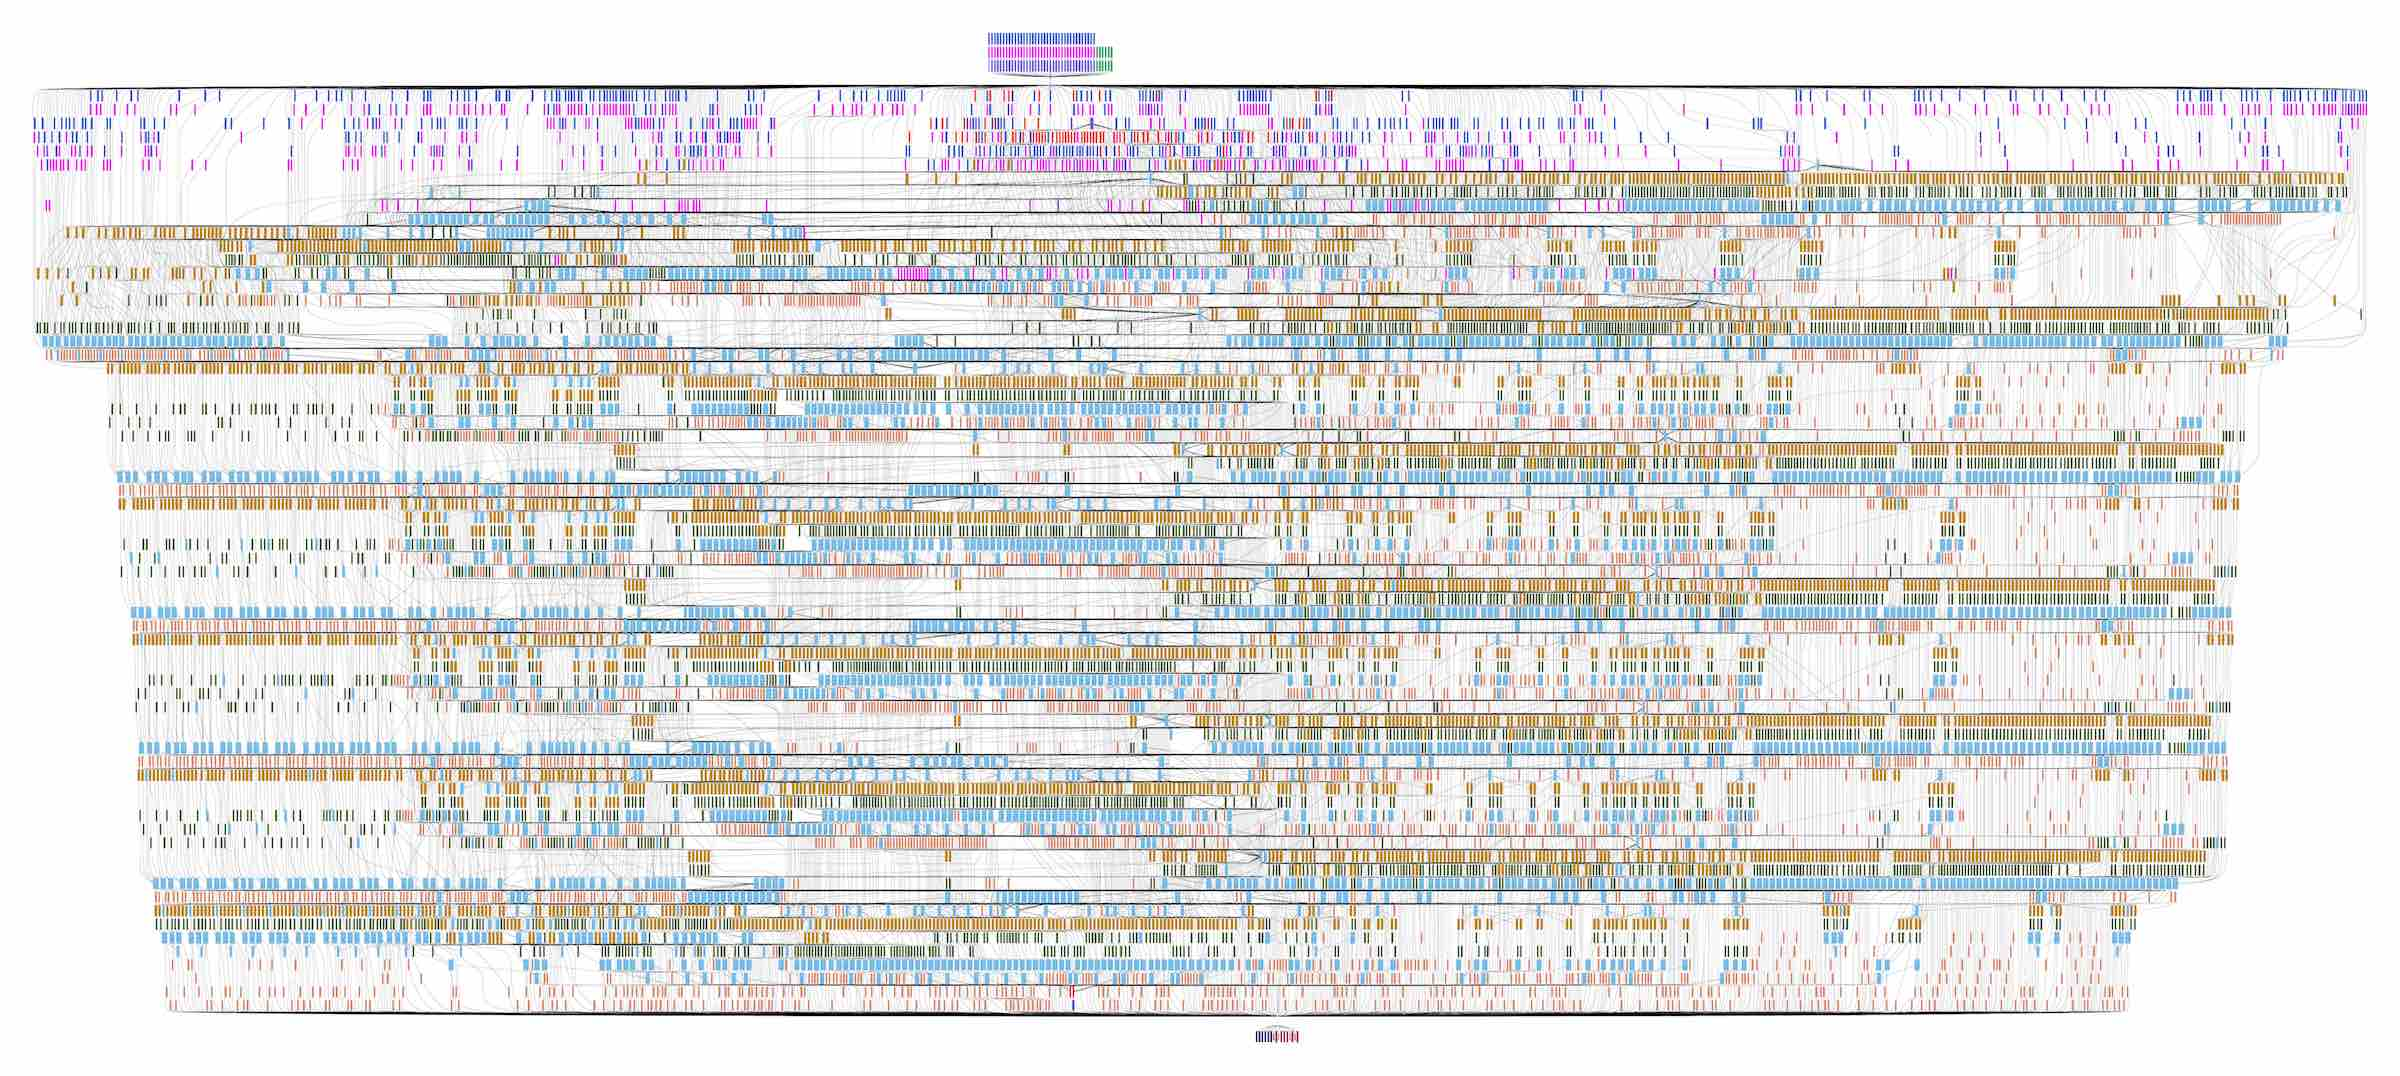
\includegraphics[width=6.5in]{projects/2.3.1-PMR/2.3.1.08-Legion/tg}
	\caption{\label{fig:task-graph}The Legion task graph for a single time step on a 
	single node.  The S3D configuration in this example is simulating n-dodecane 
	chemistry reactions in addition to the direct numerical simulation of the 
	turbulent flow.}
\end{figure}

\paragraph{Next Steps}
We will continue to focus on improving the interoperability of Legion with other programming
systems, simplifying the programming API for the Legion runtime to improve both our educational 
outreach as well as developer productivity, have regular open source releases of Legion and
also work with application teams for debugging, feature improvements and performance 
tuning.  In addition we are actively monitoring the emerging hardware technology components
that are potential targets for use in the Exascale systems that will be eventually deployed 
by both the DOE Office of Science and the NNSA. 

\clearpage
\newpage
\subsubsection{\stid{1.09} Distributed Tasking at Exascale: PaRSEC}


\paragraph{Overview}

The PaRSEC Environment provides a runtime component to dynamically execute on
heterogeneous distributed systems, and a productivity toolbox that comprises a
development framework for the support of multiple domain specific languages
(DSLs) and extensions, with debugging, trace collection, and analysis tools.
%
The PaRSEC project team is dedicated to solving two challenging and
interdependent problems facing the ECP developer community: First, how we create
an execution model that enables developers to express as much parallelism as
possible in their applications, so that those applications effectively utilize
the massive collection of heterogeneous devices that ECP machines will deploy.
Second, how we ensure that that execution model is flexible and portable enough
to actually increase the scientific productivity of those same application
developers, not only for the ECP target environments but for the foreseeable
future.
\begin{wrapfigure}{l}{.6\linewidth}
  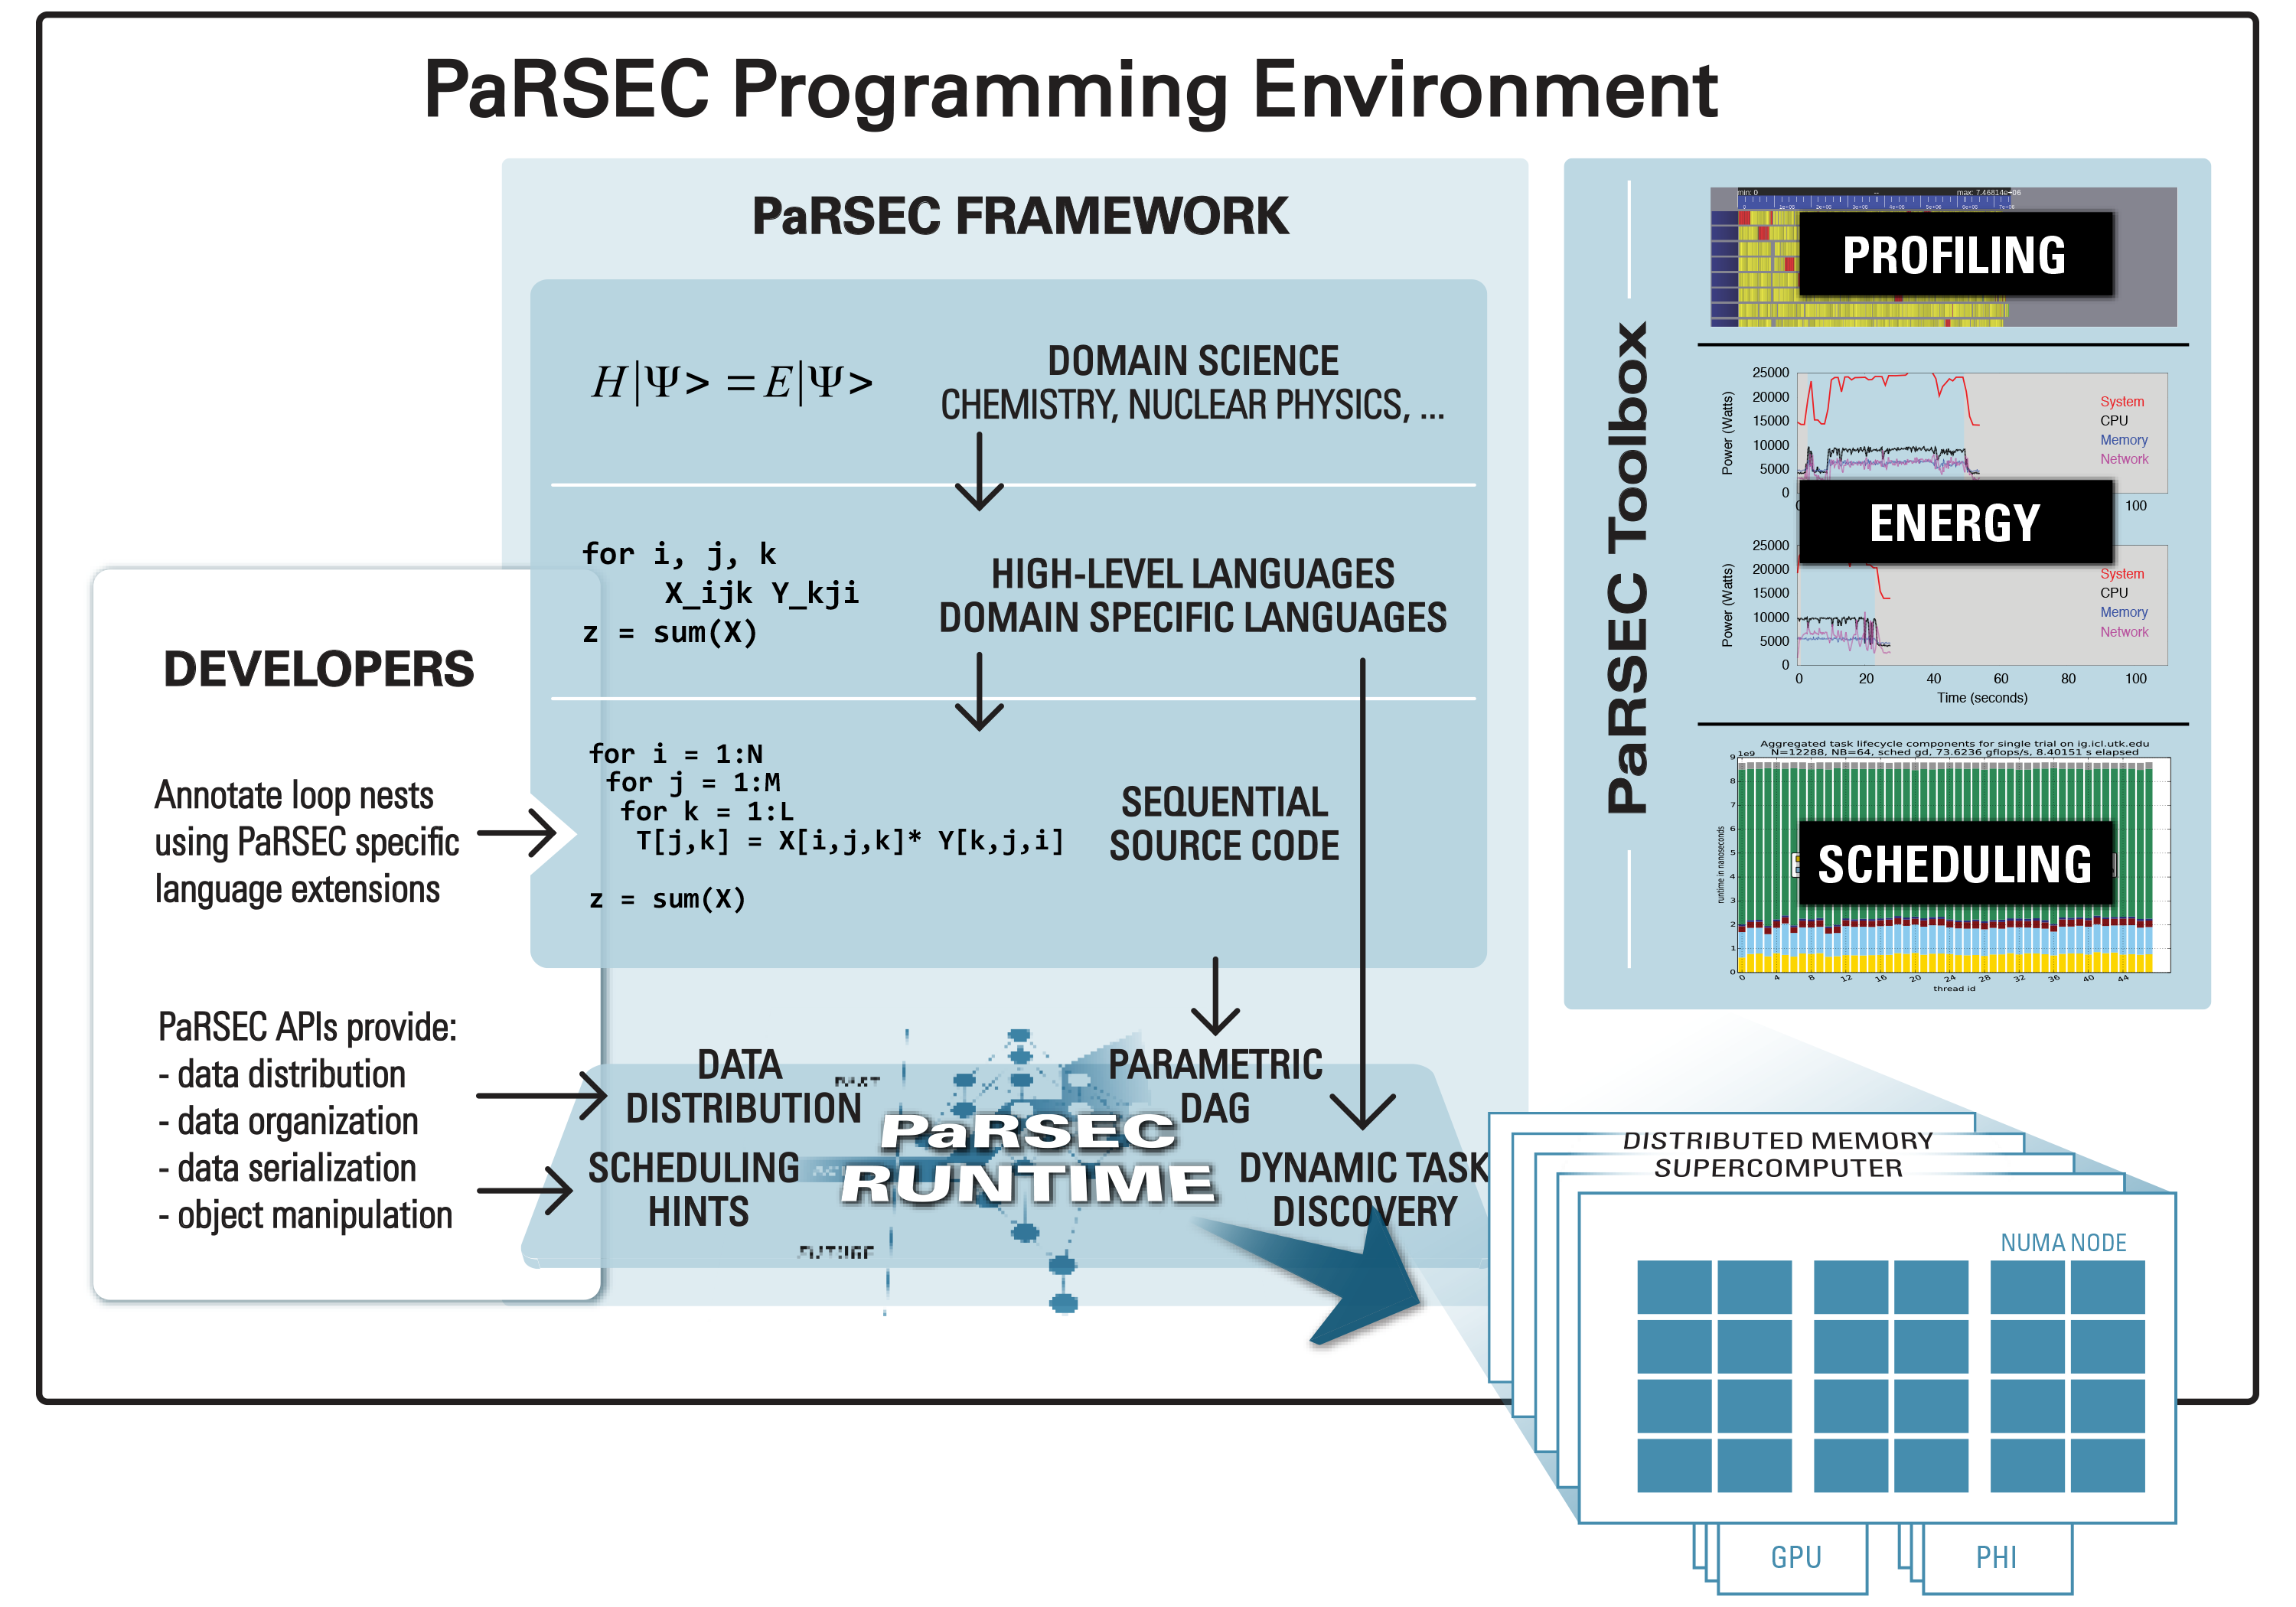
\includegraphics[scale=0.4]{projects/2.3.1-PMR/2.3.1.09-ParSEC/PaRSEC-diagram.png}
  \caption{PaRSEC architecture\label{fig:parsec}}
\end{wrapfigure}
%
PaRSEC is an open source, community-based implementation of a generic task-based
runtime that is freely available, and used by an increasing number of software
libraries. The PARSEC development team is mainly comprised of research staff at
UTK, but regular contributions from the community are provided via our presence
on GitHub and Bitbucket The project focuses on prototyping different
approaches to define task-based languages that will be able to exploit the full
range of capabilities of Exascale platforms. Without such a project, and based
on the current state of task-based runtimes, potential users will be stuck
either in fixed programming boundaries, or with particular programming
languages. The DTE project provides means to maintain a high competitiveness in the
field leading to more innovation on addressing the challenges we are facing
toward scalable, performant and Exascale ready programming paradigms.

\paragraph{Key  Challenges}
%\textit{Describe what is hard to do, why it is challenging.}

As we approach Exascale, a number of aspects of the hardware and software
environment pose challenges. First and foremost, keeping pace with the
architectural changes on current and future machines requires changes not only
on how we take advantage of the hardware capabilities, but how we reshape our
algorithms and applications to expose enough parallelism to maximize the use of
the underlying hardware. The number of nodes, threads per node, memory
hierarchies and support for increased computational capabilities (accelerators)
will continue to increase, while the currently available programming paradigms
are still struggling with parallelism at the node level.

\paragraph{Solution Strategy}
%\textit{Describe your basic strategy for addressing the challenges.}
The approach followed in PaRSEC is to provide a low-level, flexible and dynamic
runtime able not only to schedule tasks at the node level, but to handle data
transfers between different memory (both inter and intra nodes), memory
hierarchies, heterogeneous architectures with support for accelerators with a
simple programming scheme. The proposed approach envisions a middle-ground
solution, addressing both hardware and software challenges. At the hardware
level a team of dedicated developers extends PaRSEC to map it's capabilities to
the hardware and to improve it's scalability and performance. At the upper level
the interaction with the users is through building Domain Specific Languages
with the target domain scientists in mind, that will facilitate the expression
of algorithmic parallelism with familiar constructs mapped on the exposed low-level
capabilities.

\paragraph{Recent Progress}
% \textit{Describe what you have done recently.  It would be good to have some
% kind of figure or diagram in this section.}
The runtime system of PaRSEC has been extended to provide a better support of
dynamic task pools (DAGs of tasks), opening the runtime to new classes of
algorithms, such as those where the total number of tasks is a priori unknown.
% Some target applications (typically from NWChemEx) produce a dynamic DAG of
% tasks, for which the runtime cannot predict at the initialization time how many
% tasks exist, and where they will be executed.
We enabled such dynamic DAGs by removing internal constraints on how tasks are
identified and how dependencies are tracked. However, one of the missing
capabilities, the detection of the application termination, needed to be
provided explicitly.
% to determine termination of the DAG, the user had to provide the termination
% detection in a task, and broadcast explicitly that termination to all the nodes.
We added a set of termination detection algorithms to remove this step with
better efficiency, and providing a complete solution to handling dynamic DAGs.


An important aspect of the DTE project is to define and prototype scalable
domain specific languages that enable a productive expression of parallelism for
end-user communities. PaRSEC presents multiple programming interfaces
(Parameterized Task Graphs for maximum parallelism, the popular serial task
insertion dataflow model to provide direct access to the runtime). In addition
the DTE team is in close contact with application teams to define parallel
abstractions that are suitable for their domain usage. Notably, the PaRSEC team
has ongoing collaboration with the SLATE linear algebra package and NWChemEx
chemistry package teams.
The PaRSEC development team did the first step toward the integration
of their framework into the SLATE (2.3.3.09) in the context of the
shared milestone (STPM11-23). The first prototype of the application
ran in a distributed environment and showed the capability of the
SLATE library using a modern fully capable runtime system. This work
involved enhancing the insert task interface available in the ParSEC
runtime to map onto the logic of a SLATE algorithm.

\begin{wrapfigure}{l}{.5\linewidth}
  \centering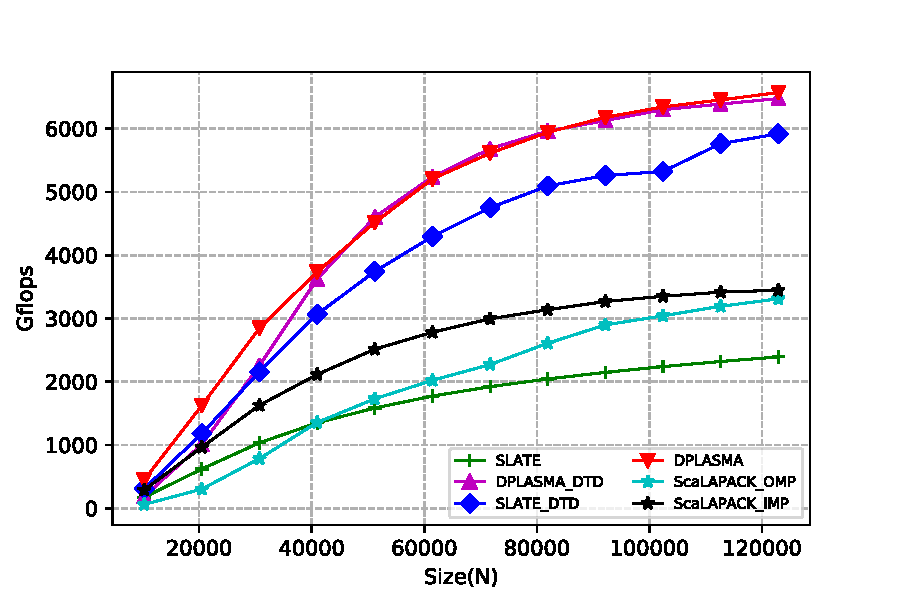
\includegraphics[scale=0.5]{projects/2.3.1-PMR/2.3.1.09-ParSEC/SLATE_inital_result_phicluster_scalapack.pdf}
  \caption{PaRSEC architecture \label{fig:slate-parsec}}
\end{wrapfigure}
%
In figure~\ref{fig:slate-parsec}, we compare the integration of SLATE
and PaRSEC against the state of the art. First against the two legacy
domain specific languages that have the capability to do linear
algebra; then against the regular SLATE using OpenMP for intra-node
parallelism, and MPI for communication; and finally against ScaLAPACK,
which is the reference for distributed linear algebra.

On the software quality side, the PaRSEC runtime has been evaluated and amended
to compile and run on all major target pre-Exascale platforms (ALCF Mira, Theta; OLCF
Titan, Summit-dev). In particular the detection of architecture specific
features on NVIDIA V100 accelerators and Power processors has been improved.
PaRSEC now includes a Spack definition file to ease the deployment on future
target systems as part of the system software SDK effort.

\paragraph{Next Steps}
%\textit{Describe what you are working on next.}

% GPU engine
A major effort at refactoring the accelerator and GPU component
of the PaRSEC runtime is ongoing. The new runtime component handles
memory transfers to/from accelerators as schedulable completion events
that can trigger asynchronously the next step of the accelerated task
and/or dependent tasks. The new engine is modular, one of the component
provides a CUDA backend optimized for NVIDIA accelerators, and a new component
will provide an OpenMP target backend for portability to other hardware.


We are improving the performance characterization system of PaRSEC to
enable users to get detailed information on the performance of their
applications that use PaRSEC as a runtime system. Part of this effort
is shared with the development of Software Defined Events in ExaPAPI
and the integration within the PaRSEC runtime.

% Task cancellation
The PaRSEC runtime will be augmented with the capability for any task
to decide that a given algorithm has no more reason to be
executed. This feature requires the runtime to properly remove any
trace of the algorithm without going into extreme solutions. We do not
want to dry run the algorithm without actually executing anything, and
we do not want to remove the task from the runtime without any
consideration for the other nodes. The solution will have to be a
local decision that will leave the runtime in a coherent state without
impeding the performance with the execution of useless tasks.


% Collective API
The detection of collective pattern at the runtime level is a hard
problem.  To enhance the insert task interface, the PaRSEC development
team will provide a communication API. It will give the developer the
capability to express communication where and when it seems fit during
the algorithm.
\newpage
\subsubsection{\stid{1.10} Kokkos Support} 

\paragraph{Overview} 
Kokkos Support provides documentation, training and community building support for the Kokkos programming model. 
To that end, the project develops programming guides, API references and tutorial material for Kokkos which is presented both as independent events and at conferences such as Supercomputing.
Kokkos Support is also responsible for setting up community interaction channels such as the Slack channels now used for user communication and fostering the GitHub interactions between Kokkos developers and users.
Finally, the project supports engagement with the C++ standard in order to further the adoption of successful Kokkos concepts into the core language. 

\paragraph{Key Challenges}
For a new programming model to be successful, a comprehensive support and training infrastructure is absolutely critical. 
Prospective users must learn how to use the programming model, current users must be able to bring up issues with the development team and access detailed documentation, and the development team of the model must be able to continue technical efforts without being completely saturated with support tasks. 
The latter point became a significant concern for the Kokkos team with the expected growth of the user base through ECP.  
Already before the launch of ECP, there were multiple application or library teams starting to use Kokkos for each developer on the core team -- a level not sustainable into the future without a more scalable support infrastructure. 
This issue was compounded by the fact that Kokkos development was funded through NNSA projects, making it hard to justify extensive support for open science applications. 

\paragraph{Solution Strategy}

Kokkos Support addresses these challenges through a number of ways. 
First and foremost, it provides explicit means for supporting all DOE ECP applications. 
A main component of that is funding for local Kokkos experts at the Sandia, Oak Ridge and Los Alamos laboratories which can serve as direct contacts for local applications and, in Oak Ridge's case, for users of the Oak Ridge Leadership Computing Facility. 
Secondly, the project develops a reusable support infrastructure, which makes supporting more users scalable and cost effective. 

The support infrastructure consists of GitHub wiki pages for the programming guide and an API reference, GitHub issues to track feature requests and bug reports, a Slack channel for direct user-to-user and user-to-developer communication, and tutorial presentations and cloud-based Kokkos hands-on exercises. 

\paragraph{Recent Progress}

Kokkos Support has successfully run multiple Kokkos bootcamps for DOE applications as well as organized a number of single day tutorials. 
At the most recent tutorial during the DOE ECP All Hands meeting, the new cloud-based hands-on infrastructure was used for the first time, allowing tutorial attendees to use GPUs on remote servers without the hassle of temporary user account administration at DOE computing facilities. 
The project also improved existing documentation and transferred it to GitHub wiki pages which are tailored for software documentation and more maintainable. 
The Slack channels usage is growing, which have seen participation from users across the DOE and Kokkos community. 
There are also more interactions on GitHub issues, including a number of pull requests volunteered from external users as a result of these interactions to improve small parts of the Kokkos implementation. 
These latter two points are a sign that the community is growing and more actively participating in advancing Kokkos, a necessary step for a more sustainable future where users may answer other users questions, and the community begins to provide new features and solutions to problems. 
 
\paragraph{Next Steps}

There are two main thrusts of development underway: the writing of a Kokkos API Reference and the development of more advanced tutorials. 
While the Kokkos Programming Guide and the Tutorial Presentations are well received, more advanced users often only want to look up the API of Kokkos features. 
Such an API reference is not yet available. Its development is under way, and we hope to have it cover the majority of Kokkos features by the end of Summer 2018. 

For tutorials, feedback provided by attendees indicate that some of the material covered in the standard tutorial is a bit too advanced for an introduction to Kokkos. On the other hand, as the number of users who have had previous exposure to Kokkos is growing, they are asking for more of the advanced features to be covered. To support both types of attendees, it is clear that splitting the tutorial into beginner and advanced sections, as well as extending the advanced section beyond what is currently covered is necessary. 

Finally, we would like to improve the accessibility of all of the resources that are being developed to support Kokkos and increase its adoption. 
Currently, all documentation, tutorials, references, and support channels are in various locations that are best suited to their differing format requirements. 
However, having a one-stop landing page where new encounters can learn about the project and current users can find the location of all available resources would increase usage of the various materials and communication channels within the community, among both developers and users.


\newpage
\subsubsection{2.3.1.11 Open MPI for Exascale (OMPI-X)}\label{subsubsect:openmpi}

%% {\itshape

%% 	\begin{enumerate}
%% 	\item Rename this file to your project WBS-projectname.tex, for example 2.3.3.01-XSDK4ECP.tex.
%% 	\item Complete this template for your project.  Limit your text to two pages, not counting citations.
%% 	\item Please avoid changing the content of main.tex.
%% 	\item Put any references in a .bib file with the same root name, for example 2.3.3.01-XSDK4ECP.bib.
%% 	\item Remember to include any image files you reference in your text.
%%     \item The files 2.3.3.01-XSDK4ECP.tex, 2.3.3.01-XSDK4ECP.bib and xSDK-diagram.jpeg are included as examples for your reference.  You can remove them from what you upload.
%% 	\end{enumerate}
%% }

\paragraph{Overview}
%% \textit{Provide an overview of your project.  You might find that the introductory text from your Fall 2017 Project Summary \url{https://confluence.exascaleproject.org/display/1ST/Fall+2017+ECP+ST+Project+Summaries} useful as a starting draft.}

The OMPI-X project ensures that the Message Passing Interface (MPI)
standard, and its specific implementation in Open MPI meet the needs
of the ECP community in terms of performance, scalability, and
capabilities or features. MPI is the predominant interface for
inter-process communication in high-end computing.  Nearly all of the
ECP application (AD) projects (93\%~\cite{Bernholdt:2017:smu-talk})
and the majority of software technology (ST) projects
(57\%~\cite{Bernholdt:2017:smu-talk}) rely on it.
%% Since its
%% inception, the MPI standard has evolved to address the changing needs
%% of massively parallel libraries and applications as well as the
%% systems on which they are run.
With the impending exascale era, the
pace of change and growing diversity of HPC architectures pose new
challenges that the MPI standard must address.  The OMPI-X project is
active in the MPI Forum standards organization, and works within it to
raise and resolve key issues facing ECP applications and libraries.

Open MPI is an open source, community-based implementation of the MPI
standard that is
%% freely available, and
used by a number of prominent
HPC vendors as the basis for their commercial MPI offerings.  The
OMPI-X team is comprised of active members of the Open MPI community,
with an extensive history of contributions to this community.
%% the development and
%% maintenance of the library.
The OMPI-X project focuses on prototyping
and demonstrating exascale-relevant proposals under consideration by
the MPI Forum, as well as improving the fundamental performance and
scalability of Open MPI, particularly for exascale-relevant platforms
and job sizes.  MPI users will be able to take advantage of these
enhancements simply by linking against recent builds of the Open MPI
library.

Without the OMPI-X project, there will be less competition and less
innovation in addressing the needs of ECP users in the critical area
of scalable, performant, and capable exascale-quality inter-process
communication capabilities.

\paragraph{Key  Challenges}
%% \textit{Describe what is hard to do, why it is challenging.}
A number of aspects of ``exascale'' levels
of computing pose serious challenges to the ``tried and true'' message
passing model presented by MPI and its implementations, including Open
MPI.
%
Keeping pace with changes in HPC architecture is a major challenge.
The MPI ecosystem (the standard and its implementations) needs to
evolve to address challenges
%% on the programming side
driven by
architectural change, as well taking advantage of new features and
capabilities.
%
As applications and libraries
%% they rely on
build up to exascale,
%% levels of computing and beyond,
the number of node, processes, and
threads required will rise significantly, whereas other key resources,
such as memory tend to go \emph{down} on a per-node, -process, or
-thread basis.  This emphasizes the importance of scalability in terms
of both performance and resource utilization.
%% to allow MPI to scale to
%% meet those needs.
%
Finally, we must work with in the much larger and broader MPI
community to find approaches to address these challenges which do not
adversely impact the capabilities, performance, or scalability for
other users of MPI and Open MPI.

\paragraph{Solution Strategy}
%% \textit{Describe your basic strategy for addressing the challenges.}
The OMPI-X project is working across a number of fronts to address
these challenges.

\emph{Runtime Interoperability for MPI+X and Beyond} MPI is
increasingly being used concurrently with other runtime environments.
This includes both ``MPI+X'' approaches, where X
%% , in the ECP
%% environment, X
is most often a threading model, such as OpenMP, as
well as the use of multiple inter-process runtimes within a single
application.  Concerns include awareness of other runtimes,
cooperative resource management capabilities, and ensuring that all
concurrently active runtimes make progress.  We will develop APIs and
demonstrate capabilities for interoperability in both MPI+X and
multiple inter-process runtime situations.

\emph{Extending the MPI Standard to Better Support Exascale
Architectures} The MPI community is considering for standardization a
number of ideas that 
%% A number of ideas under consideration by the MPI
%% community for standardization
are particularly important to supporting
the architectural and system size characteristics anticipated for
exascale.  ``Finepoints'' and ``Endpoints''
%% are approaches to
deal
with the growing use of threading for node-level concurrency, in
combination with MPI.  ``Sessions'' increases the flexibility of MPI
semantics in a number of areas, which in turn can open opportunities
for enhanced scalability, as well as easier support for
multi-component applications such as coupled multi-physics
simulations.  We will develop prototype implementations and work with
ECP teams to evaluate the ability of these approaches to address ECP
requirements in order to facilitate the standardization process.

\emph{Open MPI Scalability and Performance} As we push the scale of
both hardware and applications, we stress MPI implementations and
expose areas that need to be improved in order to improve scalability.
OMPI-X is targeting memory usage within Open MPI, as well as remote
memory access (RMA), tag matching, and other areas, for improvements
in both scalability and performance.

\emph{Supporting More Dynamic Execution Environments} We are
developing and implementing strategies to help MPI applications
better deal with topological process layout preferences
%% as well as
%% responding to
and contention in the network.

\emph{Resilience in MPI and Open MPI} Concerns about system and
application resilience increase as either scales in size.
%% (number of
%% components or MPI ranks).
We will provide implementations of the
User-Level Fault Mitigation (ULFM) and ReInit proposals currently
under discussion within the MPI Forum, as well as demonstrations of
their use, in order to help drive standardization discussions, and to
help ECP team understand how they can take advantage of these
capabilities to improve the resilience of their libraries and
applications.

\emph{MPI Tools Interfaces}  Several interfaces within the
MPI standard are primarily used to support performance and
correctness tools.
%% of various kinds.
The MPI Forum is in the process
of making significant revisions and extensions to these interfaces.
We will track the discussions in the Forum and provide prototype
implementations within Open MPI to facilitate evaluation and provide
feedback.
%% on the standardization discussions.
We will work with the
ECP community, including tool developers, to make additional data
available through the MPI\_T interface.

\emph{Quality Assurance for Open MPI}  We are enhancing the
Open MPI testing infrastructure, adding tests to reflect ECP
requirements, and instantiating routine testing on systems of
importance to ECP.

\paragraph{Recent Progress}
%% \textit{Describe what you have done recently.  It would be good to
%% have some kind of figure or diagram in this section.}
One of the first activities of the project was to conduct a survey of
ECP AD and ST projects to better understand their current and expected
usage of MPI, and look for significant issues in the MPI environment
that we might have overlooked in our planning for the project.  A
paper describing the survey results was presented at the ExaMPI 2017
workshop held in conjunction with SC17~\cite{Bernholdt:2017:smu-talk},
and will appear in a special issue of Concurrency and Computing:
Practice and Experience.  The survey has generated a great deal of
interest in the MPI community, and there are plans to expand the scope
to provide a better characterization of MPI usage around the world.

We have delivered an implementation of the User-Level Fault Mitigation
(ULFM) resilience approach, which are under consideration by the MPI
Forum for inclusion in the standard.  ULFM provides the basic building
blocks for cheap, tailored recovery capabilities within applications
and libraries using MPI.  ULFM imposes no overhead on raw
communication performance on ECP-relevant hardware.  We are now
working with several application teams to demonstrate the capabilities
it provides.

\begin{wrapfigure}{r}{4in}
\begin{minipage}[c]{2in}
\vspace{0pt}
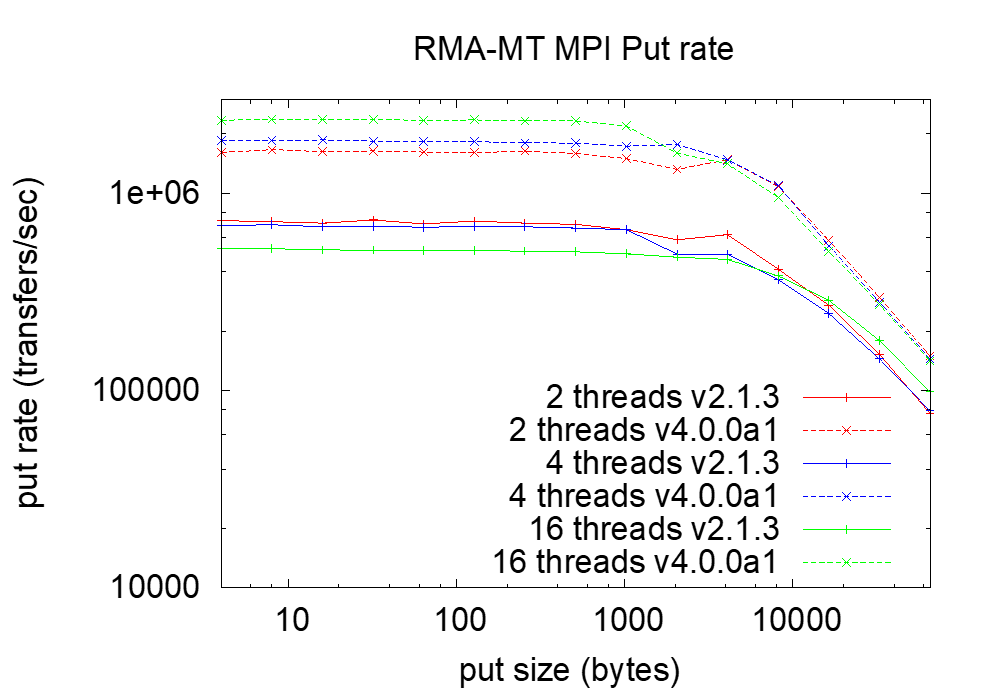
\includegraphics[width=\textwidth]{projects/2.3.1-PMR/2.3.1.11-OMPI-X/pritchard-rma-mt-put-rate.png}
\end{minipage}
\begin{minipage}[c]{2in}
\vspace{0pt}
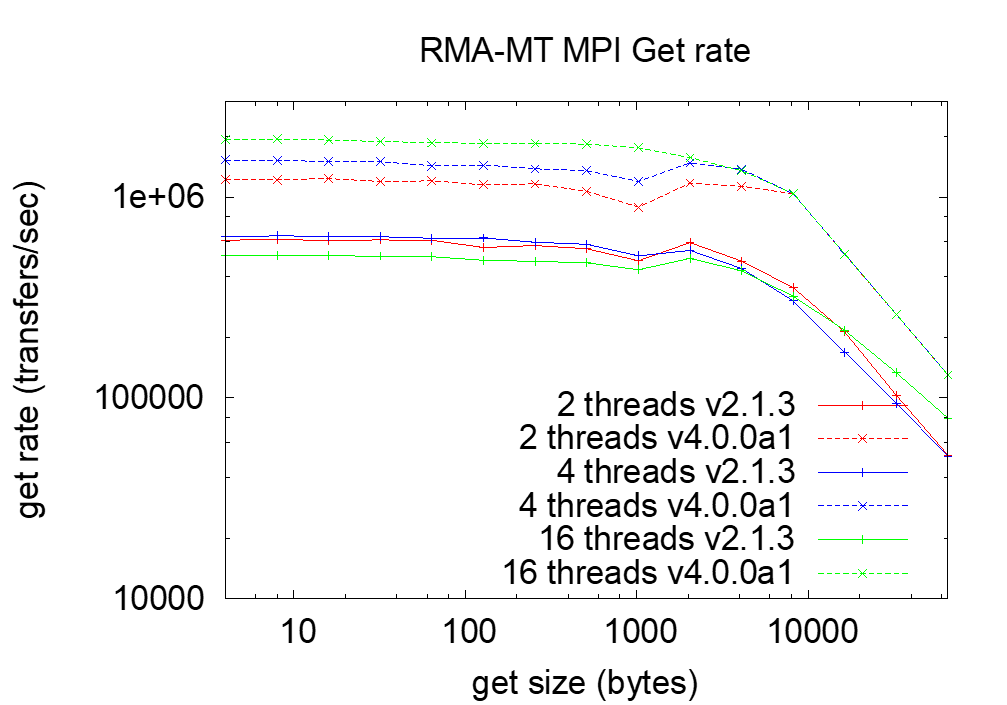
\includegraphics[width=\textwidth]{projects/2.3.1-PMR/2.3.1.11-OMPI-X/pritchard-rma-mt-get-rate.png}
\end{minipage}
\caption{Comparison of put (left) and get (right) RMA performance in a
multi-threaded context for Open MPI.  Recent OMPI-X contributions are
reflected in version 4.0.0a1 (top group of lines), in comparison with
v2.1.3.}
\label{fig:ompix-rma}
\end{wrapfigure}

We expect to be working on scalability and performance of Open MPI
throughout the project, but some early successes have been
demonstrated.  We have improved the RMA implementation so achieve
performance levels comparable to those obtained only by high tuned
implementations by vendors and significantly improved their
performance in multi-threaded contexts (Fig.~\ref{fig:ompix-rma}).  We
have also been able to improve message matching by up to 2$\times$
generally, and up to 45$\times$ on Intel Xeon Phi processors, and we
have made significant improvement to performance when MPI is used in a
multi-threaded environment.

Early work with the prototype implementation of Finepoints shows
improvements of 25\% in communication costs and 5\% in overall
execution time for one ECP mini-app.
%
Open MPI support for the MPI\_T interface has been extended~\cite{icl:957} to
provide a set of low-level counters to present a more detailed performance
characteristics map to tools and to users.
%
Finally, we have deployed the MTT testing infrastructure used by Open
MPI on ORNL's SummitDev and Summit platforms, as well as improving the
MTT system itself.

\paragraph{Next Steps}
%% \textit{Describe what you are working on next.}
We are making progress across multiple fronts, some of which has been
described above.  In FY18, we expect to complete our primary efforts
in the area of resilience in Open MPI, an implementation of the
``ReInit'' approach to complement the already completed User-Level
Fault Mitigation (ULFM) capability.  Both approaches continue to be
debated within the MPI Forum, but we are hopeful that demonstrations
based on our implementations can help bring these discussions to a
conclusion. Early in FY19, we will also be delivering a formal
proposal and prototype implementation of the ``Finepoints'' approach to
supporting environments with large numbers of threads.

\newpage
\subsubsection{\stid{1.12} Runtime System for Application-Level Power Steering on Exascale Systems} 

\paragraph{Overview} 
Power remains a critical constraint for Exascale. As we design supercomputers at larger scales, power becomes an expensive and limited resource. Inefficient management of power leads to added operational costs as well as low scientific throughput. Although hardware advances will contribute a certain amount towards achieving high energy efficiency, they will not be sufficient, creating a need for a sophisticated system software approach. Significant advances in software technologies are thus required to ensure that Exascale systems achieve high performance with effective utilization of available power. Distributing available power to nodes while adhering to system, job and node constraints involves complex decision making in software. 

The ECP PowerSteering project is developing a \emph{job-level} power management runtime system that will optimize performance of Exascale scientific applications transparently under power and/or energy constraints. Existing research efforts, including Conductor and Adagio, are being actively integrated into Intel's GEOPM runtime system, an ongoing open source effort led by Intel. This integration expands GEOPM?s capabilities with the latest research while providing a production-grade, industry-supported open source solution. By developing new platform plugins, this project also supports upcoming target platforms and paradigms for ECP beyond the Intel architectures, and incorporates task-based programming models such as Legion. By being both configurable and cross-platform, GEOPM will help applications achieve maximum performance under a power constraint. 

This project is essential for ECP because it enables Exascale applications to operate safely with optimal performance under power and energy constraints. This project is also essential for building a sophisticated hierarchical software stack proposed by the ECP Argo and ECP Flux projects. Additionally, the project fulfills an essential need for ECP by enabling vendor and academic collaborations that provide for accelerated adoption of best practices and better interoperability at scale.  By leveraging the GEOPM software developed in this project, compute centers can safely operate under power and energy constraints while maximizing performance and scientific throughput. 


\paragraph{Key Challenges}
Power management in software is challenging due to the dynamic phase behavior of applications, processor manufacturing variability, and the increasing heterogeneity of node-level components. While several scattered research efforts exist, a majority of these efforts are site-specific, require substantial programmer effort, and often result in suboptimal application performance and system throughput. Additionally, these approaches are not production-ready and are not designed to cooperate in an integrated manner. A holistic, generalizable and extensible approach is still missing in the HPC community, and a goal for the ECP PowerSteering project is to provide a solution for this technology gap. 

Another set of challenges come from portability issues. Existing solutions are targeted toward specific Intel microarchitectures as well as programming models. Additionally, some of the existing solutions  violate the specified power budget before reaching a steady state, resulting in power fluctuations as well as unsafe operation. As part of this project, we strive to provide portability as well as safe operation using both hardware-level and application-level information for adaptive configuration selection and critical path analysis.

\paragraph{Solution Strategy}
Our solution is to develop a job-level runtime system (Intel GEOPM) that can operate transparently to user applications, and can also cooperate with HPC resource managers and node-level tools. We are taking a two-pronged approach. First, we are working toward consolidating existing research efforts from the community to develop high-quality plugins for GEOPM that can be deployed at Exascale. In parallel, we are developing new algorithms in GEOPM to address other Exascale challenges such as heterogeneity and variation. While GEOPM already provides some baseline algorithms, the existing capabilities are not programmer transparent and not sufficient for Exascale. Our advanced algorithms analyze critical paths of scientific applications transparently, balance power between different components intelligently, and provide mechanisms to capture fine-grained application semantics through Caliper. Additionally, these advanced algorithms will support non-Intel architectures such as IBM/NVIDIA and novel task-based programming models such as Legion, which are critical for portability in the future. We also intend for GEOPM to be a part of a holistic power management stack that does dynamic, hierarchical power management and works closely with resource managers such as SLURM or Flux.  In order to accomplish portability and smooth integration, we are closely collaborating with ECP Argo and ECP Flux projects, with University of Arizona, and with Intel and IBM. 

\paragraph{Recent Progress}
Recently, we achieved two milestones in March 2018. The first was to update the power model for our plugin to incorporate application phases and manufacturing variation, and the second milestone was to support task-based programming models in GEOPM. We developed an offline power/performance model based on processor characterization over codes with broad spectrum of compute and memory-boundedness at different processor power caps. We also updated the configuration space exploration to use this model to adjust per-MPI rank performance measurements over each computation phase. 

We are now working on testing and evaluation of our framework with the new model and collecting new data on the Quartz cluster at LLNL. Some early results are presented in Figure \ref{fig:MG}. The figure shows the compute phase of MG.C, where the runtime system uses a non-linear power-performance model during the configuration exploration phase to account for manufacturing variability. For our second milestone, we developed an MPI + Legion + GEOPM interoperability benchmark that allows us to use GEOPM for dynamic power management of task-based models. 

\begin{figure}[t]
	\centering
	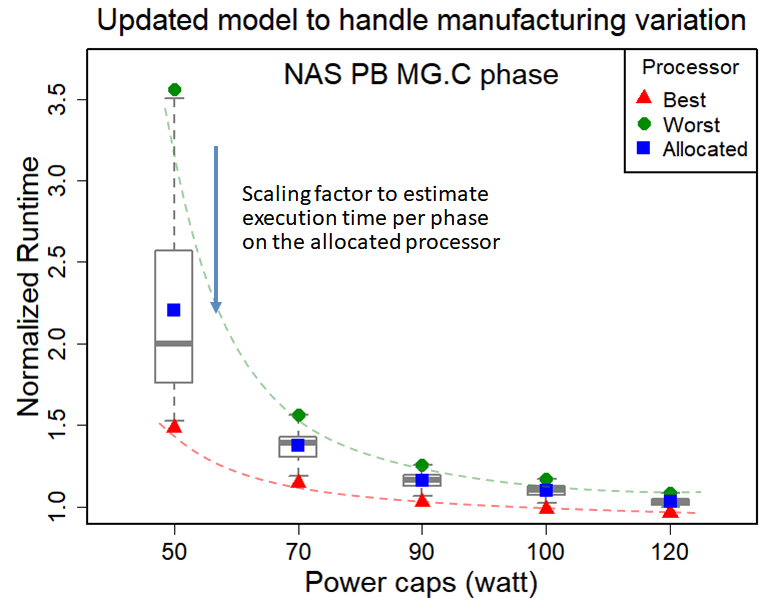
\includegraphics[scale = 0.6]{projects/2.3.1-PMR/2.3.1.12-Power-Steering/power_model.png}
	\caption{Non-linear power-performance model in use for MG.C during configuration exploration phase for the runtime system}
	\label{fig:MG}
\end{figure}


\paragraph{Next Steps}
We will continue our research and development work as planned toward the September 2018 milestones. More specifically, we are working on porting GEOPM to non-Intel architectures (IBM Power8 or Power9, and NVIDIA GPUs are candidates). We will also enhance our variation-aware and phase aware model with advanced machine learning and statistical techniques. We also plan to improve the overhead of the configuration exploration function by selecting configurations that minimize sampling overhead without a significant impact on the prediction accuracy of the power model especially at lower power budgets. 

One of our current challenges is to gain access to non-Intel architectures such as IBM Power8/Power9 and NVIDIA GPUs with elevated privileges that are required for power management. We are working with LLNL to gain such access. Additionally, for our Legion work, we are working toward understanding mappers as well as task distribution better in order to determine the spatial and temporal aspects of power management with GEOPM plugins. We are also looking into S3D application code as part of our Legion power model  exploration. Lastly, we are looking into adding Spack support for installing GEOPM. 


\newpage
\subsubsection{\stid{1.13} SOLLVE} \label{subsubsect:sollve}


\paragraph{Overview} 

OpenMP is a   directive-based API for shared-memory and accelerator systems. It
is supported by a stable community of vendors, research labs, and academics who
participate in the efforts of the  OpenMP Architecture Review Board; it   is
also the most used API for intra-node programming in ECP applications.
Implementations are available in all DOE LCFs, and a variety of programming
tools are available to support OpenMP application development. The mission of
the SOLLVE project is to further enhance the OpenMP specification and
implementations to meet the performance and productivity goals of ECP
applications. We directly interact with DOE end-users in order to understand
their application software requirements. We will develop OpenMP solutions for
ECP needs; propose features for standardization; produce prototype
implementations of new features to support their rapid adoption; develop and
deliver a verification and validation (V\&V) suite to assess implementations and
enable evaluations by DOE  facilities, and deliver a high-quality,  robust ECP
OpenMP implementation in the LLVM compiler framework. Attaining high levels of
single-node performance and meeting performance portability needs will only be
possible via enhancements to OpenMP in such areas as data motion and placement
in complex memory  hierarchies, efficiency in the context of C++,  and features
that allow the creation of performance portable code. SOLLVE plays a critical
role in identifying, implementing, promoting, and deploying key functionality
that will enable ECP application developers to reach their goals using OpenMP.
We will demonstrate the high impact of new features via their use in selected
ECP applications.

\paragraph{Key  Challenges}
%\textit{Describe what is hard to do, why it is challenging.}
The SOLLVE project addresses a number of key challenges faced by DOE facilities,
application groups and scientists. The first of these is the gap between
existing OpenMP functionality and user requirements. This problem is largely
exacerbated by ever increasing complexity and heterogeneity of computing
systems.
The second challenge is to suitably evolve the OpenMP specification to satisfy
the identified requirements. This process involves coordinating with vendors
and other members of OpenMP's language committee  to reach consensus on the scope of the API, syntax and semantics of new features.
The third challenge addressed by the SOLLVE project is performance portability.
Current hardware and software trends 
\cite{exascale-roadmap.ijhpca.2011}
 have shown that
pre-Exascale and Exascale systems will be extremely heterogeneous, and may 
consist of  diverse architectures such as
CPUs, GPUs, FPGAs, among others. Programmatically, this means that 
memory hierarchies will be even deeper, and multiple levels and types
of parallelism will have to be exposed, extracted and mapped onto these systems 
to achieve suitable performance levels. 
This naturally places heavy emphasis on application readiness, where APIs such as 
OpenMP will need to address 
performance portability to serve the critical role
of abstracting hardware and software complexities.
Finally, the last challenge is to fully assess the quality of delivered
OpenMP implementations, their compliance with the specification and potential
divergence that, if unidentified, could can lead to undesired program behavior.
% and, ultimately, errors
%that can consume significant amount of resources to repair.


\paragraph{Solution Strategy}
The challenges discussed here are addressed by 5 major thrust areas, which
we describe below as part of the SOLLVE process:
%\textit{Describe your basic strategy for addressing the challenges.}

\begin{enumerate}
\item {\bf Application requirements}
The first step of the SOLLVE process consists in collecting user requirements
from relevant and representative ECP applications (e.g. QMCPACK or Lattice QCD).
Collected requirements are then converted to use-cases which are then handed
to the OpenMP Standard Committee.
\item {\bf OpenMP specification evolution}
This thrust area is responsible of translating use-cases to new OpenMP
features to be introduced into the standard. In this phase, the semantics
of the new capabilities are defined and formalized, followed by early
prototypes in one or more OpenMP implementations (either vendor or open
source solutions). Broadly, the bulk of new features fall into the areas
of accelerator, affinity, tasking or memory management.
\item {\bf Lightweight OpenMP runtime}
SOLLVE is committed to deliver an open source, lightweight and scalable
OpenMP implementation (the BOLT runtime) that will fulfill ECP needs.
This deliverable serves two key objectives: i) early access to a stable 
implementation; and ii) risk mitigation.
\item {\bf LLVM }
This compiler infrastructure is ideal for 
delivering high-quality and deployable OpenMP implementations.
Our effort enhances the LLVM framework by introducing compiler transformations
that leverage both prototyped OpenMP features and those introduced
in OpenMP 4.5. User adoption of new OpenMP capabilities could vary from
months to years. Thus, delivering compiler technology that automatically transforms
user's code targeting the new OpenMP functionality (e.g. target offloading with
data mappers), represents high return value for ECP in terms of time and
resources. 
\item {\bf Validation and verification (V\&V)} This thrust focuses on
designing and implementing a benchmark suite that allows to assess the coverage
and standard compliance of several OpenMP implementations (LLVM, BOLT, IBM XL,
NVIDIA, etc). In addition, a ticket system for bug reporting and inquiries has
also been deployed to facilitate interaction with end users.
\end{enumerate}

\paragraph{Recent Progress}
Figure \ref{fig:sollve-update} shows the latest progress on the 5 core SOLLVE
thrust areas. We note that the {\bf training and outreach} activity is a
cross-cutting effort which includes resources from the SOLLVE project and
external partners, namely collaborators from Lawrence Berkeley National
Laboratory, Oak Ridge, University of Delaware and other academic institutions.
In addition to the above updates, a number of articles have also been published
as part of the SOLLVE effort \cite{openmp-tr6,zinenko.cc.2018,osti_1429981,DBLP:conf/sc/MishraLKFC17}.

\begin{figure}[t]
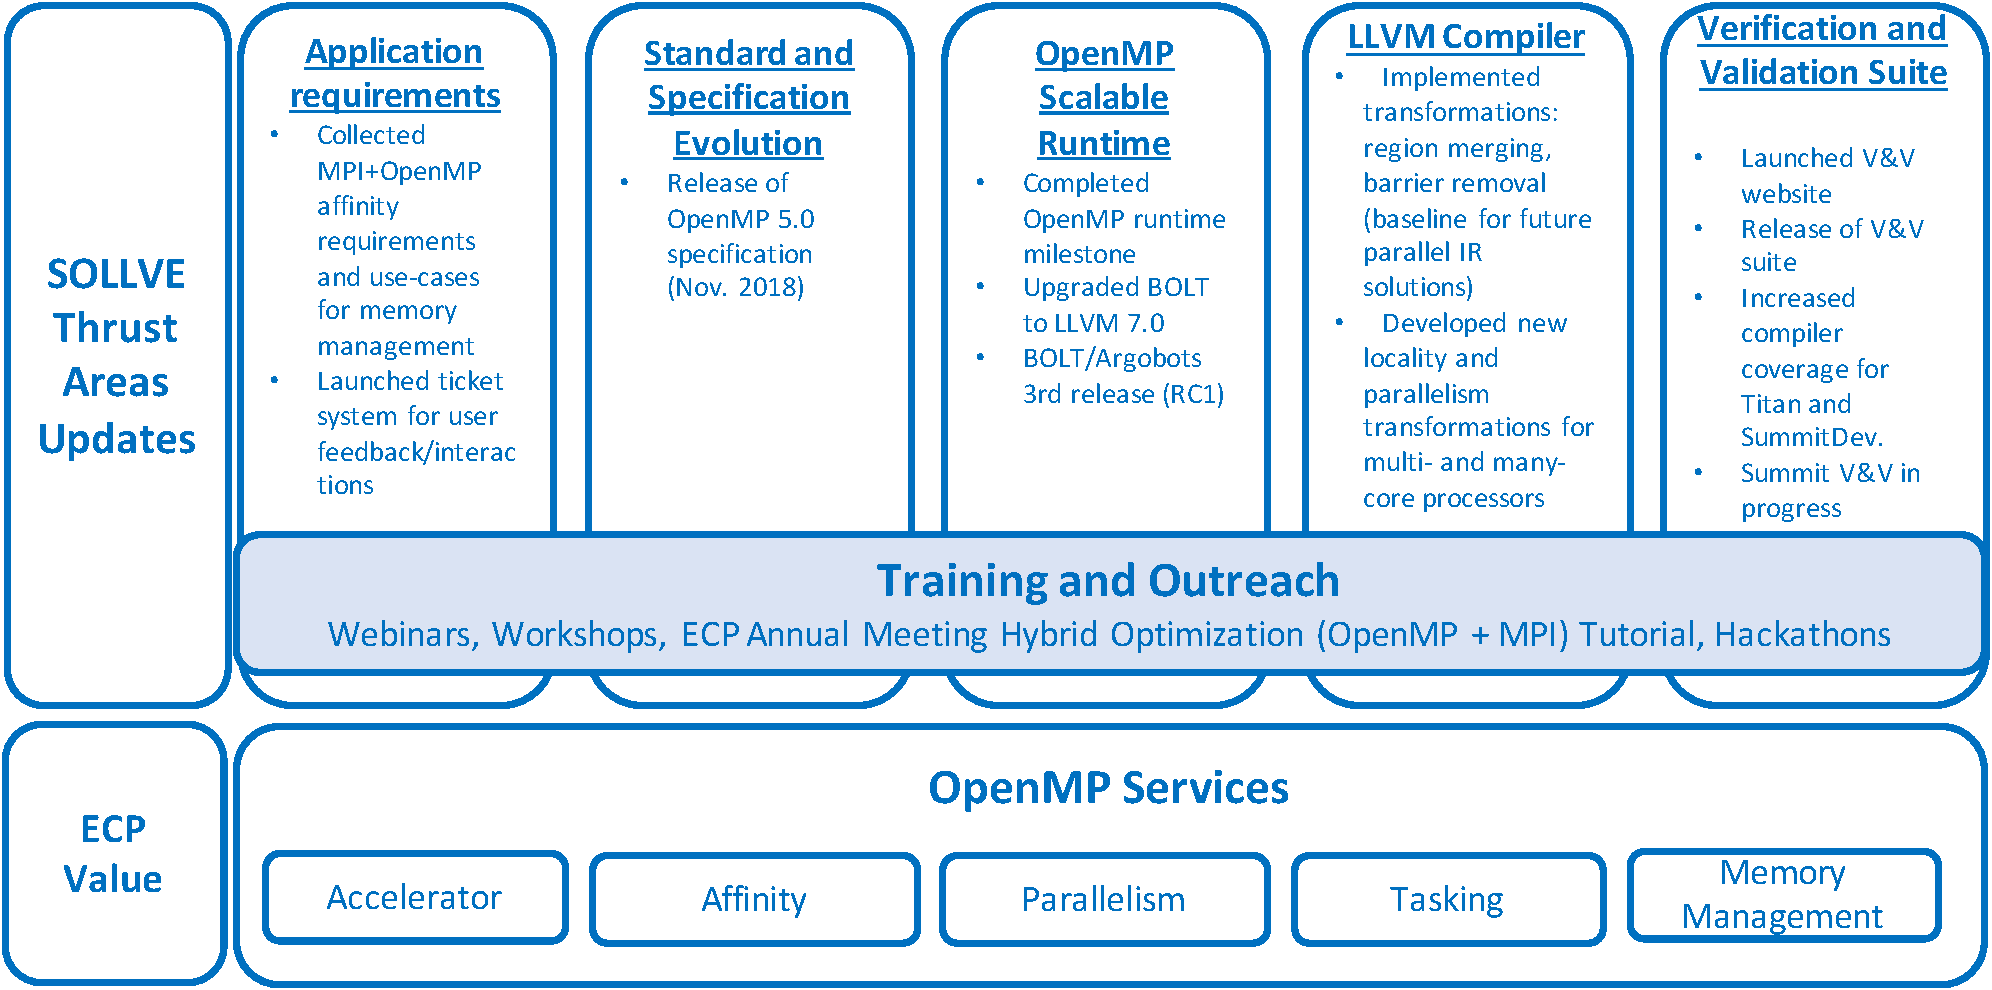
\includegraphics[width=0.98\linewidth,height=8cm]{projects/2.3.1-PMR/2.3.1.13-SOLLVE/SOLLVE-progress}
\caption{\label{fig:sollve-update}SOLLVE thrust area updates}
\end{figure}

\paragraph{Next Steps}
As next steps planned for SOLLVE we have
\begin{itemize}
\item Applications: gather more requirements for memory management API and concurrent parallel construct; prepare and coordinate OpenMP webinar focusing on memory management, deep copy and tasking.
\item OpenMP standard: Next face-to-face meeting in May; ratify and vote latest memory management features, mappers and parallelism descriptors
\item OpenMP runtime: design and implement high-level interface for passing scheduling/blocking hints
\item LLVM compiler: develop new optimizations leveraging prototype parallel-IR; refine Clang based implementation of data layout transformations; evaluate new compiler transformations on Intel KNL and ARM architectures
\item V\&V suite: identify performance critical kernels from selected applications; prepare release for SC18; coordinate suite deployment with CORAL systems.
\end{itemize}


\newpage
\subsubsection{\stid{1.13} Argobots: Flexible, High-Performance Lightweight Threading }

\paragraph{Overview}

Efficiently supporting massive on-node parallelism demands highly
flexible and lightweight threading and tasking runtimes. At the
same time, existing lightweight abstractions have shortcomings while
delivering generality and specialization.  Our group at Argonne
developed a lightweight, low-level threading and tasking framework,
called Argobots.  The key focus areas of this project are: (1) To
provide a framework that offers powerful capabilities for users to
allow efficient translation of high-level abstractions to low-level
implementations. (2) To provide interoperability with other
programming systems such as OpenMP and MPI as well as with other
co-located I/O services. (3) To provide a programming framework that
manages hardware resources more efficiently and reduce interference
with co-located applications.

\paragraph{Key Challenges}

Several user-level threading and tasking models have been proposed in
past to address the shortcomings of OS-level threads, primarily with
respect to cost and flexibility. Their lightweight nature and flexible
generic interface play an important role at managing efficiently the
massive concurrency expected at the Exascale level.  Existing
user-level threading and tasking models, however, are either too
specific to applications or architectures or are not as powerful or
flexible. Existing runtimes tailored for generic use \cite{GNUPth,
  PLDI97_Taura, COSET05_Thibault, COB14_Nakashima, MTAAP08_Wheeler,
  PPoPP99_Taura, SenSys06_Dunkels, TBB1, EuroPar08_Perache} are
suitable as common frameworks to facilitate portability and
interoperability but offer insufficient flexibility to efficiently
capture higher-level abstractions, while specialized runtimes
\cite{ATC02_Adya, SolarisThreads, SOSP03_von_Behren, StateThreads,
  PLDI07_Li, MTAAP09_Porterfield, WMPP05_Cuvillo, IntelOMP, Nanos++,
  LCPC96_Kale, PACT14_Treichler} are oriented to a specific
environment.

\paragraph{Solution Strategy}

Argobots offers a carefully designed execution model that balances
generality of functionality with providing a rich set of controls to
allow specialization by end users or high-level programming models.
Argobots honors this high degree of expressibility through three key
aspects:

\begin{enumerate}

\item Argobots distinguishes between the requirements of different
  \emph{work units}, which are the most basic manageable
  entities. Work units that require private stacks and context-saving
  capabilities, referred to as \textit{user-level threads} (ULTs, also
  called \textit{coroutines} or \textit{fibers}), are fully fledged
  threads usable in any context.  \emph{Tasklets} do not require
  private stacks. They are more lightweight than ULTs because they do
  not incur context saving and stack management overheads.  Tasklets,
  however, are restrictive; they can be executed only as atomic work
  units that run to completion without context switching.

\item Work units execute within OS-level threads, which we refer to as
  \emph{execution streams} (ESs). Unlike existing generic runtimes,
  ESs are exposed to and manageable by users.

\item Argobots allows full control over \emph{work unit
  management}. Users can freely manage scheduling and mapping of work
  units to ESs and achieve the desired behavior.

\end{enumerate}

In order to ensure fast critical paths despite the rich set of
capabilities, Argobots was designed in a modular way to offer
configuration knobs and a rich API that allow users to trim
unnecessary costs.

\paragraph{Recent Progress}

The proposed lightweight, low-level threading and tasking framework
that is designed as a portable and performant substrate for high-level
programming models or runtime systems is called as Argobots. The
design of the Argobots is as follows:

\begin{enumerate}

\item \textbf{Execution Model:} Figure~\ref{fig:sollve-argobots}
  illustrates the execution model of Argobots. Two levels of
  parallelism are supported: ESs and work units. An ES maps to one OS
  thread, is explicitly created by the user, and executes
  independently of other ESs. A work unit is a lightweight execution
  unit, a ULT or a tasklet, that runs within an ES.  There is no
  parallel execution of work units within a single ES, but work units
  across ESs can be executed in parallel.  Each ES is associated with
  its own scheduler that is in charge of scheduling work units
  according to its scheduling policy.

\item \textbf{Scheduler:} Argobots provides an infrastructure for
  stackable or nested schedulers, with pluggable scheduling policies,
  while exploiting the cooperative non-preemptive activation of work
  units. Localized scheduling policies such as those used in current
  runtime systems, while efficient for short execution, are unaware of
  global policies and priorities. Argobots allows each ES to have its
  own schedulers.  To execute work units, an ES has at least one main
  scheduler ($S_{M}$).  A scheduler is associated with one or more
  \textit{pools} where ready ULTs and tasklets are waiting for their
  execution.  Stacking schedulers is achieved through pushing
  schedulers into a pool. When a higher-level scheduler pops a
  scheduler from its pool, the new scheduler starts its execution
  (i.e., scheduling).  Once it completes the scheduling, control
  returns to the scheduler that started the execution. To give control
  back to the parent scheduler, a scheduler can also yield.  To
  support plugging in different scheduling policies, all schedulers,
  including the main scheduler, and pools are replaceable by
  user-provided alternatives.

\item \textbf{Primitive Operations:} Argobots defines primitive
  operations for work units such as \textbf{Creation}, \textbf{Join},
  \textbf{Yield}, \textbf{Yield\_to}, \textbf{Migration} and
  \textbf{Synchronizations}. Since tasklets are used for atomic work
  without suspending, most operations presented here---except
  creation, join, and migration---apply only to ULTs.

\end{enumerate}

Argobots is implemented in C language.  An ES is mapped to a Pthread
and can be bound to a hardware processing element (e.g., CPU core or
hardware thread).  Context switching between ULTs can be achieved
through various methods, such as \texttt{ucontext},
\texttt{setjmp}/\texttt{longjmp} with
\texttt{sigaltstack}~\cite{ATC00_Engelschall}, or Boost library's
\texttt{fcontext}~\cite{fcontext}. A pool is a container data
structure that can hold a set of work units and provides operations
for insertion and deletion. Argobots relies on cooperative scheduling
of ULTs to improve resource utilization. That is, a ULT may
voluntarily yield control when idle in order to allow the underlying
ES to make progress on other work units.

\begin{figure}[htb]
  \centering
  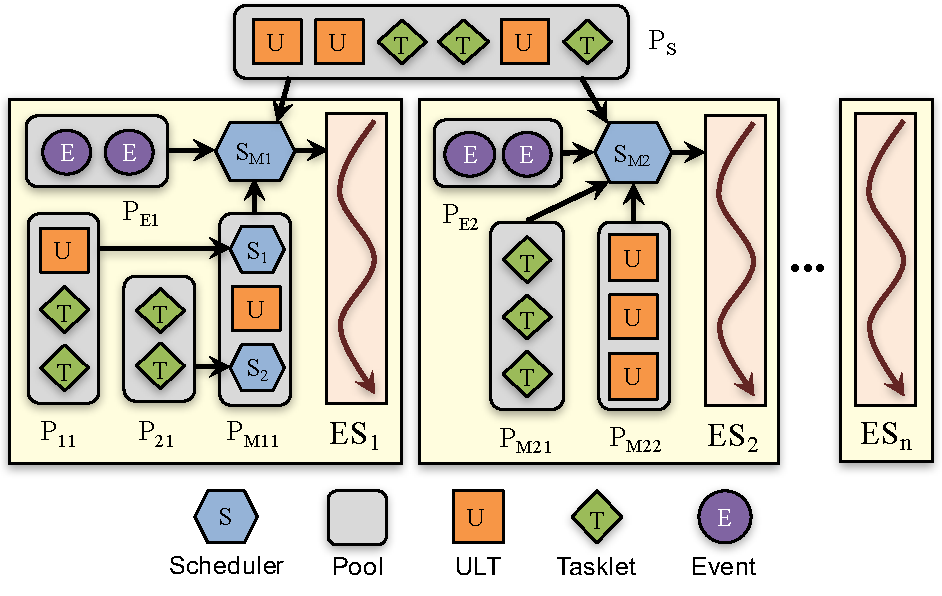
\includegraphics[height=3in]{projects/2.3.1-PMR/2.3.1.13-SOLLVE/SOLLVE-ARGOBOTS.pdf}
  \caption{\label{fig:sollve-argobots}Argobots execution model}
\end{figure}

\paragraph{Next Steps}

We studied three use cases of Argobots for higher level runtimes as
follows:

\begin{enumerate}

\item \textbf{OpenMP over Argobots:} Our OpenMP runtime implemented
  over Argobots (called BOLT) outperforms other OpenMP implementations
  because of using lightweight work units. We plan to leverage the
  supported features.

\item \textbf{Interoperability with MPI:} We investigated an MPI
  runtime that interoperates with Argobots ULTs instead of OS-level
  threads. The runtime has been shown to be subject to lock management
  issues directing us to further work on lock implementation.

\item \textbf{Colocated I/O services:} The most straightforward way to
  utilize Argobots within an I/O service daemon is to create a new ULT
  to service each incoming I/O request.  We implemented two small
  extension libraries to help support this use case.  The first,
  \emph{abt-io} and the second is \emph{abt-snoozer}. Further the
  service routines are decomposed into smaller discrete event-driven
  routines with disjoint stacks, a technique known as \emph{stack
    ripping}~\cite{ATC02_Adya}.  Presently, Argobots significantly
  reduce the development, debugging, and maintenance burden for system
  services and needs further investigations.

\end{enumerate}

\newpage
\subsubsection{\stid{1.13} BOLT: Lightning Fast OpenMP}\label{subsubsect:bolt}

\paragraph{Overview}

OpenMP is central for several applications that target Exascale,
including ECP applications, to exploit on-node computational
resources.  Unfortunately, current production OpenMP runtimes, such as
those that ship with Intel and GNU compilers, are inadequate for the
massive and fine-grained concurrency expected at the Exascale level.
These runtimes rely on heavy-handed OS-level threading strategies that
incur significant overheads at fine-grained levels and exacerbate
interoperability issues between OpenMP and internode programming
systems, such as MPI and OpenSHMEM.  Our solution is a production
quality OpenMP runtime (called BOLT) that leverages user-level threads
instead of OS-level threads (e.g., Pthreads).  Due to their
lightweight nature, managing and scheduling user-level threads incurs
significantly less overhead.  Furthermore, interoperability between
BOLT and internode programming systems opens up new optimization
opportunities by promoting asynchrony and reducing hardware
synchronization (atomics and memory barriers).  Initial studies on
this proposal can be found in \cite{ccgrid, ppopp}.  This report
briefly summarizes the issues in OpenMP runtimes that rely on OS-level
threading, describes BOLT as the solution to this challenge, the
current status in the BOLT effort, and the next steps for further
improvements.

\paragraph{Key Challenges}

The growing hardware concurrency in High Performance Computing (HPC)
cluster nodes is pushing applications to chunk work more fine-grained
to expose parallelism opportunities.  This is often achieved through
nested parallelism either in the form of parallel regions or explicit
tasks.  Nesting parallel regions can potentially cause
oversubscription of OS-level threads to CPUs and thus lead to
expensive OS-level thread management.  Such heavy costs usually
outweigh the benefits of increased concurrency and thus compels the
OpenMP programmer to avoid nested parallel regions altogether.  Such
workaround, however, not only causes poor resource utilization from
insufficient parallelism but is also not always possible.  For
instance, the nested level could be outside the control of the user
because it belongs to an external library that also uses OpenMP
internally.  Internode programming systems, such as MPI and OpenSHMEM,
are not aware of OpenMP semantics, such as the notion of an OpenMP
task.  What these internode systems understand is the low-level
threading layer used by OpenMP, such as Pthreads.  This threading
layer serves as the interoperability medium between OpenMP and the
internode programming system and has a direct impact on performance.
For instance, when OpenMP threads are allowed to concurrently perform
internode communication, the interoperability layer dictates how
thread safety and progress on communication is handled.  It is
notoriously known that OS-level thread safety in production MPI
libraries suffers significant performance issues.  Despite the recent
improvements to OS-level thread safety in MPI libraries, the
state-of-the-art performance results are still indicating serious
scalability issues.  While continues progress on improving OS-level
thread safety in these important internode programming systems is
crucial for traditional interoperability, we propose in this work
exploring an orthogonal direction that assumes a more lightweight
interoperability layer.

\paragraph{Solution Strategy}

Both fine-grained parallelism and interoperability issues suffer from
the heavy nature of working at the level of OS threads.  Our solution
to both challenges leverages user-level threads.  Using user-level
threads as the underlying threading layer for the OpenMP runtime
offers a significantly better trade-off between high concurrency and
thread management overheads.  This allows users to generate
fine-grained concurrency and oversubscription without worrying about
the performance collapse that is observed in current OpenMP runtimes.
Our OpenMP runtime, BOLT, is derived from the LLVM OpenMP runtime and
leverages Argobots, a highly optimized lightweight threading library,
as its underlying threading layer.  OpenMP threads and tasks are
spawned as Argobots work units and nested parallel regions are managed
through an efficient work-stealing scheduler.  Furthermore, new
compiler hints are being investigated to allow reducing thread
management overheads even further.  Interoperability improvements have
also been demonstrated by having BOLT interoperate with an MPI library
(MPICH) through the Argobots threading layer rather than OS-level
threads.  Results showed that this approach allows better
communication progress and outperforms the traditional Pthreads-level
interaction.

\paragraph{Recent Progress}

The development of BOLT went through several steps that involved
developing or optimizing various aspects.  The first step was to fork
BOLT from the upstream LLVM OpenMP runtime (https://openmp.llvm.org)
and replace the Pthreads layer with a basic Argobots design.  Next, we
implemented advanced scheduling strategies to improve the performance
of BOLT under fine-grained nested parallelism regimes.
Figure~\ref{fig:sollve-bolt} shows the development of BOLT.  The
following step was to investigate ways to reduce thread management
overheads by exploiting application knowledge.  By taking into account
the suspension likelihood of a thread or task (e.g., yield execution
on a blocking I/O operation), we have extended Argobots to leverage
such information and incorporated these features into the BOLT
runtime.  With respect to interoperability with MPI, we have
investigated the shortcomings of current interoperability models at
the implementation as well as standard specification levels.  We have
investigated the benefits of having a more lightweight
interoperability layer through Argobots using BOLT as the OpenMP
runtime and MPICH as the MPI library and demonstrated encouraging
results.  BOLT and Argobots have been subject to two releases and our
latest progress results have been published in the prestigious IEEE
Transactions on Parallel and Distributed Systems journal and some
results have been described in an ECP report.

\begin{figure}[htb]
  \centering
  \vspace{2.0ex}
  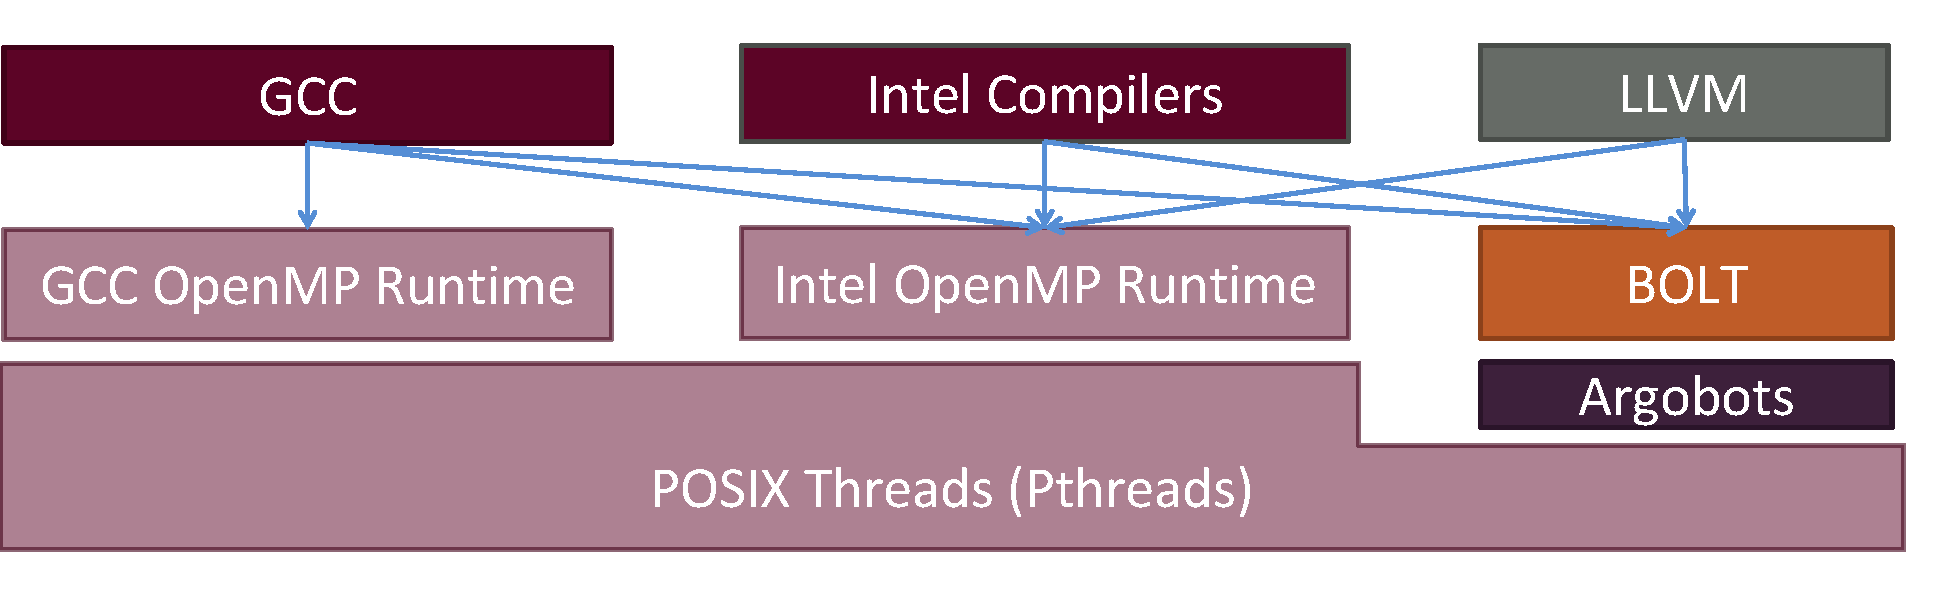
\includegraphics[width=0.9\columnwidth]{projects/2.3.1-PMR/2.3.1.13-SOLLVE/SOLLVE-BOLT.pdf}
  \caption{\label{fig:sollve-bolt}Pictorial representation of development of BOLT}
  \vspace{2.0ex}
\end{figure}

\paragraph{Next Steps}

Some aspects of BOLT require further work and investigation.  In the
following we enumerate some of the key aspects under progress:

\begin{enumerate}

\item User hints to lower thread management overheads previously
  described were only implemented at the runtime level.  We plan to
  work with the compiler team of the SOLLVE project to integrate these
  hints at the compiler level.

\item Only benchmarks and a few application cases have been used for
  evaluation purposes.  We plan to investigate a wider range of
  applications, including ECP ones, to evaluate the effectiveness of
  our solution and potentially discover new areas of needed
  improvement.

\item The interoperability results between BOLT and MPI were
  encouraging but still preliminary.  We are planning on doing more
  extensive evaluation of this interoperability layer with benchmarks
  and applications and potentially implement improvement if
  scalability is unsatisfactory.

\item Finally, we plan to perform more rigorous robustness testing
  with validation and test suites as well as with fully-fledged
  applications and proxy-application for as much coverage as possible.

\end{enumerate}

\newpage
\subsubsection{UPC++} 
\paragraph{Overview} 
The UPC++ project is developing a C++ library
that supports Partitioned Global Address Space (PGAS) programming~\cite{Bachan:paw17}.
The UPC++ project began in 2012 with a prototype designated V0.1, described in \cite{zheng:ipdps14}.
We are revising the library under the auspices of the DOE's Exascale Computing
Project, to meet the needs of applications requiring PGAS support.
UPC++ is well-suited for implementing elaborate distributed data structures where
communication is irregular or fine-grained. The UPC++ interfaces for
moving non-contiguous data and sending Remote Procedure Calls (RPC)
are composable and closely resemble those used in modern C++.

UPC++ is needed for ECP because it delivers low-overhead communication that runs
at close to hardware speeds, embracing 
interest by vendors in the PGAS model because it 
efficiently matches the RDMA mechanisms offered by
network hardware and on-chip communication between distinct address
spaces.  
Because ECP applications rely on irregular representations
to improve accuracy and conserve memory, the UPC++ library provides
an essential ingredient for the ECP software stack.  It will enable
effective scaling in Exascale software by minimizing the work funneled
to lightweight cores, avoiding the overhead of long, branchy serial
code paths, and supporting efficient fine-grained communication.  The
importance of these properties is exacerbated by application trends;
many ECP applications require the use of adaptive meshes, sparse
matrices, dynamic load balancing, or similar techniques.  UPC++'s
low-overhead communication mechanisms can maximize injection rate and
network utilization, tolerate latency through overlap, streamline
unpredictable communication events, minimize synchronization, and
efficiently support small- to medium-sized messages arising in such
applications.  UPC++ will enable the ECP software stack to exploit
the best-available communication mechanisms, including novel features
being developed by vendors.  This library offers a complementary,
yet interoperable, approach to MPI with OpenMP, enabling developers to
focus their effort on optimizing performance-critical communication.

\paragraph{Key  Challenges}

As the result of technological trends, the cost of data motion is steadily increasing relative to that of computation.  To reduce communication costs we need to 
either reduce the software overheads or hide  communication behind available computation. UPC++ addresses both strategies.
To reduce software overheads, UPC++ takes advantage of the GASNet-EX communication library's \cite{gasnet-spec}
low-overhead communication as well as access to any special hardware
(see the accompanying report on GASNet-EX, which is being co-designed).
UPC++ supports asynchronous communication via classic one-sided communication
(i.e. puts and gets) and remote procedure calls, to support communication hiding.


% A challenge in the ECP-ST effort is to maintain interoperability among run times,
% that invoke the back end to carry out communication. The difficulty is that each
% backend operates under the assumption that it "owns" the network.
% But many ECP applications employ (or will under ECP) multiple runtimes;
% thus interoperability is of paramount concern.
% Our approach is conservative; so long as entries and exits between different
% models is sufficiently coarse grained, then it is feasible to synchronize
% at a barrier at each transition.

\paragraph{Solution Strategy}

The UPC++ project has two primary thrusts:
\begin{enumerate}
\item \textbf{Increased performance through reduced communication costs:} The
UPC++ programmer can expect communication to run at close to hardware speeds.
Asynchronous execution enables an application to hide communication behind
available computation.

\item \textbf{Improved productivity:}  UPC++'s treatment of asynchronous
execution relies on futures and promises, and these simplify the management of
asynchrony.

\end{enumerate}

The PGAS one-sided communication employed by UPC++ (get/put)
benefits application  performance by mapping tightly onto the RDMA
communication supported by the communication network. GASNet-EX provides the
thin middleware
needed to enable this model to run at close to hardware speeds, across platforms ranging from laptops to supercomputers.
One-sided communication also has another benefit.
It decouples synchronization from data motion,
avoiding synchronization overheads of two-sided communication (e.g. message passing).

UPC++'s Remote Procedure Call, which is built on GASNet Active Messages,
provides additional control over asynchronous execution, by enabling
the programmer
to execute procedure calls on remote processors.
RPC is useful in managing access to complicated irregular data structures,
and in expressing asynchronous task execution.

UPC++ addresses productivity via one-sided data motion, remote procedure calls,
and via the provision of futures.
Futures enable the programmer
to capture data readiness state, which is useful in making scheduling decisions, 
via continuations, to execute asynchronously as dependencies become
satisfied. Chaining and conjoining
of asynchronous operations simplify treatment of their completion.



\paragraph{Recent Progress}

symPACK is a direct linear solver for symmetric positive definite sparse matrices.
Originally written using the legacy UPC++ V0.1, we have recently ported symPACK to
use the latest release of UPC++ V1.0. Our experiments conducted on NERSC Edison
confirm that the new UPC++ version preserves the performance of the symPACK solver.


\begin{figure}[htb]
%  \captionsetup{format=centering}
	\centering
	%\includegraphics[width=6in]{sympack-perf}
  \subfloat[\textbf{Push} -- MPI two-sided communication\newline\textbf{Pull} -- UPC++: RPC + RMA Get when ready\newline 2 variants with and without event driven scheduling]{
    \label{fig:sympack:comm}
	  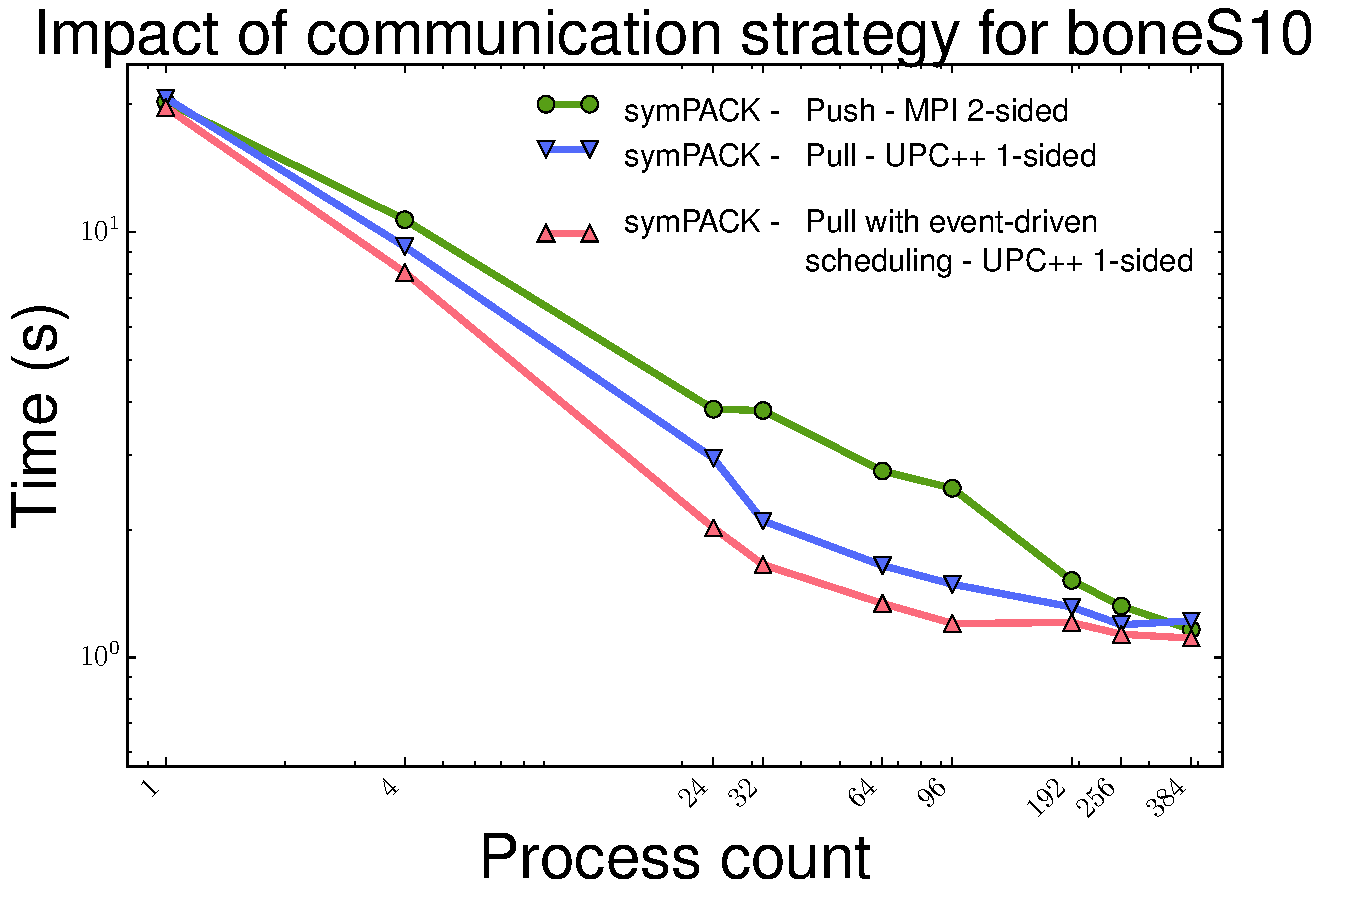
\includegraphics[width=3in]{projects/2.3.1-PMR/2.3.1.14-UPCxx-GASNet/ss_boneS10_comm.pdf}
  }
  \subfloat[Strong scaling of symmetric solvers\newline(Factorization time only)]{
    \label{fig:sympack:scaling}
	  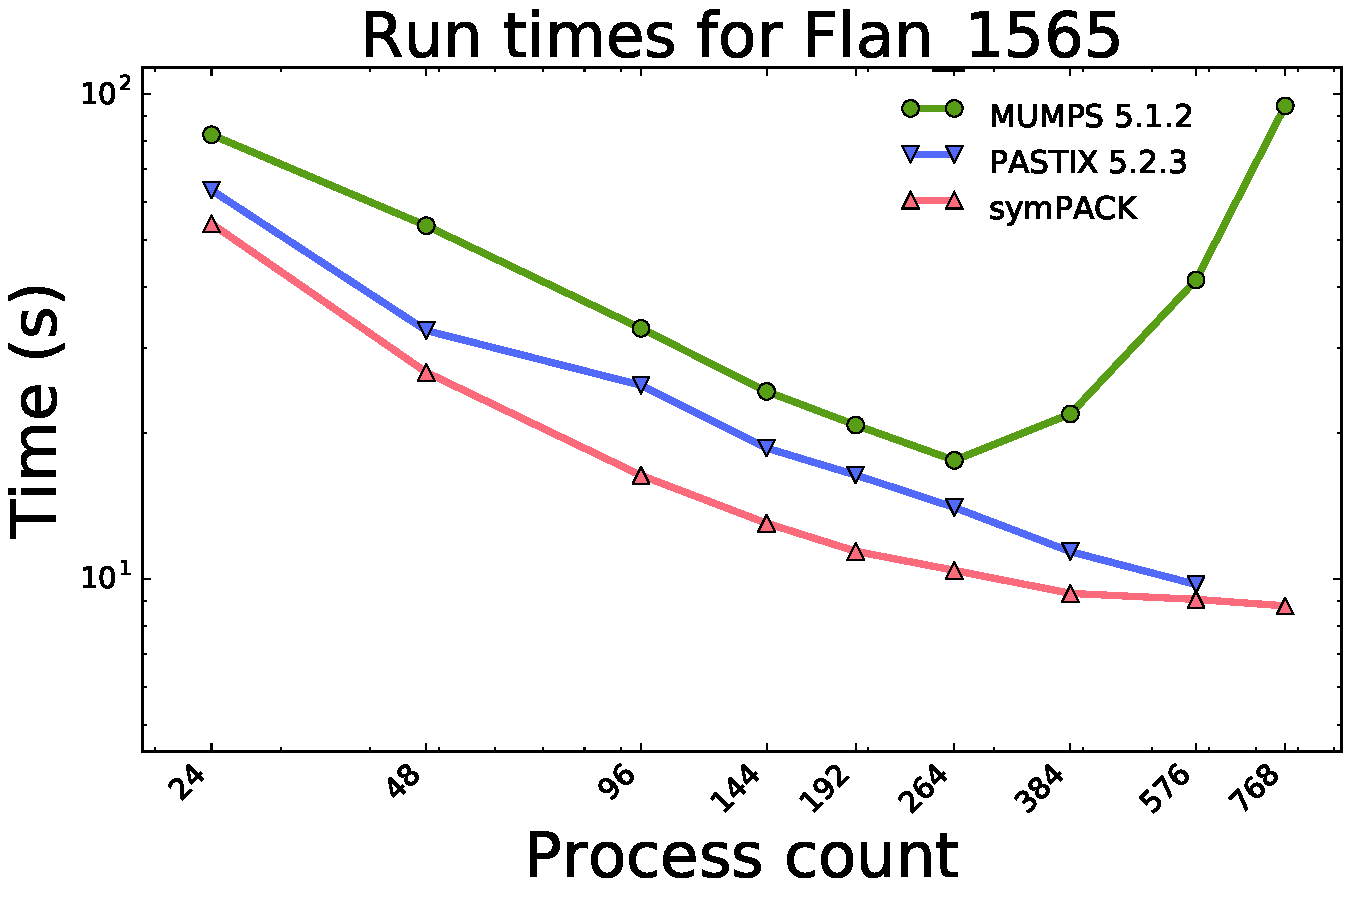
\includegraphics[width=3in]{projects/2.3.1-PMR/2.3.1.14-UPCxx-GASNet/ss_Flan_1565_complex.pdf}
  }
  \caption{\label{fig:sympack-perf}\textbf{Performance of the symPACK solver using UPC++ V1.0} }
\end{figure}



The first experiment, depicted in Fig.~\ref{fig:sympack:comm} compares the performance of three implementations of symPACK:
\begin{itemize}
  \item a \textbf{Push} strategy (the sender ``pushes'' the outgoing message
as soon as possible) using non-blocking MPI two-sided messages,
  \item a \textbf{Pull} strategy (sender ``notifies'' with RPC, receiver RMA gets when ready) using one-sided UPC++ RPC and RMA get,
  \item the same \textbf{Pull} strategy using one-sided UPC++ RPC and RMA get, combined with an event-driven dynamic scheduling policy.
\end{itemize}
UPC++ allows symPACK to implement an efficient Pull strategy using one-sided operations in a simple and efficient fashion.
This implementation surpasses the performance of the original MPI two-sided variant.
Fig.~\ref{fig:sympack:scaling} compares the strong scalability, on NERSC Edison, of symPACK with other state-of-the-art solvers
for sparse symmetric matrices. symPACK can be seen to significantly outperform
the other solvers on this particular problem, a trend which can be observed on most matrices from the SuiteSparse
matrix collection.

%Figure~\ref{fig:sympack-perf} illustrates the benefits of the PGAS model implemented by UPC++ (Mathias' results) .


% Figure~\ref{fig:dht-perf} illustrates the benefits of UPC++'s remote atomics capability with a distributed hash table implementation.
% \begin{figure}[htb]
	% \centering
	% \includegraphics[width=6in]{dht-perf}
	% \caption{\label{fig:dht-perf} {\bf CAPTION GOES HERE STEVE} }
% \end{figure}



\paragraph{Next Steps}


Our next efforts are:
\begin{enumerate}
\item \textbf{Team-aware APIs:} Teams are a mechanism for grouping ranks.
Team-aware APIs  will be developed to enable teams to be used not only in
collective communication (see below) but also in distributed objects,
and certain modes of accessing global shared storage.

\item \textbf{Support for non-blocking collectives:} UPC++ supports a small number
of collectives, and this set will be expanded to accommodate the needs of our
application partners. Support for teams will also be included.
	
	
\end{enumerate}

\newpage
\subsubsection{\stid{1.14} GASNet-EX}
\paragraph{Overview} 

The Lightweight Communication and Global Address Space Support project (Pagoda)
is developing GASNet-EX~\cite{gasnet-site}, a portable high-performance communication layer
supporting multiple implementations of the Partitioned Global Address Space
(PGAS) model.
GASNet-EX clients include Pagoda's PGAS programming interface UPC++~\cite{Bachan:paw17,upcxx-site}
 and the Legion Programming
System~\cite{bauer2012legion,legion-site} (WBS~2.3.1.08).

GASNet-EX's low-overhead communication mechanisms are designed to maximize
injection rate and network utilization, tolerate latency through
overlap, streamline unpredictable communication events, minimize
synchronization, and efficiently support small- to medium-sized
messages arising in ECP applications.  GASNet-EX enables the ECP
software stack to exploit the best-available communication mechanisms,
including novel features still under development by vendors.  The
GASNet-EX communications library and the PGAS models built upon it
offer a complementary, yet interoperable, approach to MPI with OpenMP,
enabling developers to focus their effort on optimizing
performance-critical communication.

We are co-designing GASNet-EX with the UPC++ development team with
additional input from the Legion and
(non-ECP) Cray Chapel~\cite{chapel-chapter,chapel-site} projects.

\paragraph{Key  Challenges}

Exascale systems will deliver exponential growth in on-chip parallelism and
reduced memory capacity per core, 
increasing the importance of strong
scaling and finer-grained communication events.  
Success at Exascale demands that
software needs to minimize the work performed by lightweight cores and avoid the
overhead of long, branchy serial code paths; 
this motivates a requirement for efficient
fine-grained communication.
These problems are exacerbated by application trends; many of the ECP applications require
adaptive meshes, sparse matrices,
or dynamic load balancing.
All of these characteristics favor the use of
low-overhead communication mechanisms that
can maximize injection rate and network utilization, tolerate latency through
overlap, accommodate unpredictable communication events, minimize synchronization,
and efficiently support small- to medium-sized messages. The ECP software stack
needs to expose the best-available communication mechanisms, including novel
features being developed by the vendor community.

\paragraph{Solution Strategy}

The PGAS model is a powerful means of addressing these
challenges and is critical in building other ECP programming systems,
libraries, and applications.  We use the term {\em PGAS} for models that support
one-sided communication, 
including contiguous and non-contiguous remote memory access (RMA) operations such as put/get
and atomic updates. Some of these models also include support for remote function invocation.
GASNet-EX~\cite{gasnet-lcpc18} is a communications library that provides the foundation for implementing
PGAS models, and is the successor to the widely-deployed GASNet library.
We are building on over 15 years of experience with the GASNet~\cite{gasnet-spec,gasnet-site}
communication layer to provide production-quality implementations that include
improvements motivated by
technology trends and application experience.  

The goal of the GASNet-EX work is to provide a portable, high-performance GAS
communication layer for Exascale and pre-Exascale systems, addressing the challenges
identified above.
GASNet-EX provides interfaces that efficiently match the RDMA capabilities of modern
inter-node network hardware and intra-node communication between distinct address spaces.
New interfaces for atomics and collectives have enabled offload to current
and future network hardware with corresponding capabilities.
These design choices and their implementations supply the low-overhead communications
mechanisms required to address the requirements of Exascale applications.

\begin{figure}[htb]
  \centering
  \subfloat[8-byte RMA Latencies\label{fig:rma-lat-bars}]{
     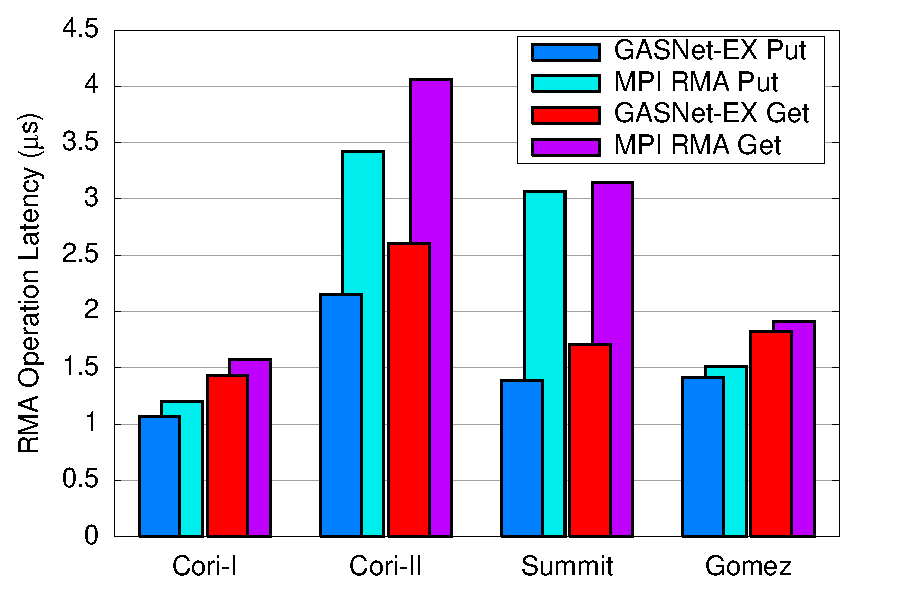
\includegraphics[width=0.432\textwidth]{projects/2.3.1-PMR/2.3.1.14-UPCxx-GASNet/latency_bars.pdf}
  }
  \subfloat[Summit Flood Bandwidth\label{fig:summit-bw}]{
     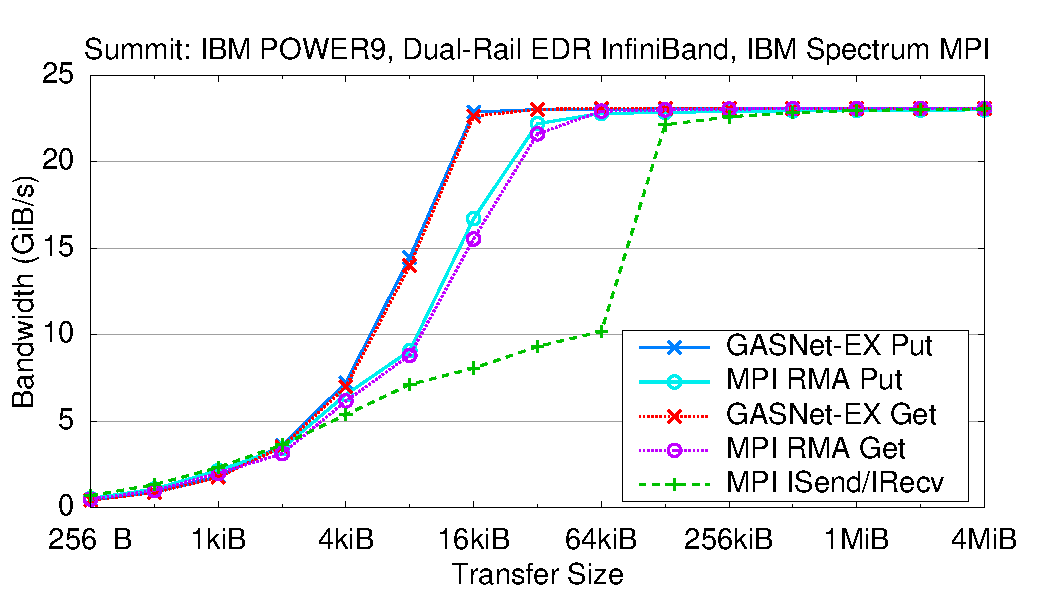
\includegraphics[width=0.504\textwidth]{projects/2.3.1-PMR/2.3.1.14-UPCxx-GASNet/Summit-slide-BW.pdf}
  }
  \caption{\label{fig:gasnet-ex-rma} Selected GASNet-EX vs. MPI RMA Performance Results}
\end{figure}

Figure~\ref{fig:gasnet-ex-rma} shows representative results from a
paper~\cite{gasnet-lcpc18} comparing
the RMA performance of GASNet-EX with MPI on multiple systems including
NERSC's Cori and OLCF's Summit%
\footnote{The paper's results from Summitdev
have been replaced by more recent (June 2019) results from OLCF's newer Summit system.}.
These results demonstrate the ability of a PGAS-centric runtime to
deliver performance as good as MPI, and often better.
%
The paper presents experimental methodology and system descriptions, which are
also available online~\cite{gasnet-site}, along with results for additional
systems.

Figure~\ref{fig:rma-lat-bars} shows the latency of 8-byte RMA Put and Get operations on
four systems, including two distinct networks and three distinct MPI
implementations.
%
GASNet-EX's latency is 6\% to 55\% better than MPI's on Put and 5\% to 45\%
better on Get.
%
Algorithms sensitive to small-transfer latency may become practical in PGAS
programming models due to these improvements relative to MPI.

Figure~\ref{fig:summit-bw} shows flood bandwidth of RMA Put and Get over the
dual-rail InfiniBand network of OLCF's Summit.
GASNet-EX's bandwidth is seen to rise to saturation at smaller
transfer sizes than IBM Spectrum MPI, with the most pronounced differences
appearing between 4KiB and 32KiB.
%
Comparison to the bandwidth of MPI message-passing (dashed green series) illustrates the
benefits of one-sided communication, a major feature of PGAS models.


\paragraph{Recent Progress}

Work on GASNet-EX in the past year has covered several distinct areas.

Co-design work is on-going with the UPC++, Legion and Chapel developers.  These
interactions are bi-directional, guiding design and implementation decisions
made in GASNet-EX as well as in the client runtimes.
%
Recent work~\cite{gasnet-reassembly} for the Cray Aries network has yielded
significant performance improvement on systems of importance to UPC++ and Legion.
Specifically, implementation of a new target-side reassembly protocol improved
AM Long end-to-end latency by up to 33\%, and the effective bandwidth by up to
49\%, while also enabling asynchronous source completion that drastically reduces
injection overheads.

We have begun work to improve interoperability of GASNet-EX and MPI within the
same executable.  Together with the Exascale MPI project (WBS~2.3.1.07) we have
developed an initial implementation of a small library to manage cooperative
progress of multiple communications runtimes.  We have demonstrated the ability
of this library, with suitable calls added to GASNet-EX and MPICH, to resolve
two canonical examples of the class of deadlock it is meant to prevent.

We have completed work to leverage features of the InfiniBand network
present in OLCF's Summit.  One such development is modifications to fully
utilize the multiple InfiniBand network ports (a.k.a ``rails'') in a Summit
node.  Another is use of Mellanox's ``ODP'' (On-Demand Paging) to provide
efficient and robust RDMA transfers to and from memory in a processes' stack
and dynamic heap.

\paragraph{Next Steps}

Our next efforts include:
\begin{enumerate}

\item \textbf{Device (GPU) Memory Support}.
GASNet-EX's RMA APIs have been designed to enable hardware offload of
transfers to and from GPU memories (\textit{e.g.} use of GPUDirect).
Near-future work includes implementation of this capability for OLCF's
Summit.  This work includes adding support for multiple
communications endpoints and multiple memory segments, which also provide
benefit to multi-threaded runtimes by reducing contention for shared resources.

\item \textbf{Specialization for InfiniBand}.  Network-specific implementations
of new GASNet-EX features for the InfiniBand network will provide performance
benefits on systems such as OLCF's Summit.  The benefits of such specialization
for the Cray Aries network has been demonstrated previously~\cite{gasnet-aries}.

\item \textbf{Client-Driven Tuning}.  In collaboration with authors of client
runtimes using GASNet-EX (most notably UPC++ and Legion) and their users (such
as ExaBiome), we will continue to identify and address any significant
bottlenecks or performance anomalies which are discovered.

\end{enumerate}

\newpage
\subsubsection{\stid{1.15} Enhancing Qthreads for ECP Science and Energy Impact} 


\paragraph{Overview} 

``Enhancing Qthreads for ECP Science and Energy Impact'' is a project that aims to improve the performance of applications that use multithreading with communication, e.g., MPI.  Most ECP applications are using this combination of programming models, with the Kokkos or RAJA performance portability libraries and/or the OpenMP API for multithreading.  This project supports the Kokkos ECP software project and OpenMP from the underlying runtime layer to deliver thread-scalable performance to those applications.  To that end, our projects is developing techniques to incorporate support for better network concurrency into the multithreading runtime system.

\paragraph{Key  Challenges}
Our project addresses the challenge of scalably coupling multithreaded parallelism on the many-core node with communication such as MPI, which has traditionally performed poorly in multithreaded mode.  The key challenge arises when multiple threads make communication calls, and those calls must be serviced by the MPI implementation and NIC.  Existing solutions, such as MPI\_THREAD\_MULTIPLE, are often plagued by synchronization overheads.  Even the best vendor MPI implementations incur high overheads when the number of threads exceeds the number of hardware contexts in the NIC. 
While current mechanisms are insufficient even for today's systems, emerging interconnect technologies expose even more network parallelism that must be exploited to maximize performance for Exascale.

\paragraph{Solution Strategy}

Unlike previous approaches, we attack the problem not only from the communication side (MPI), but with assistance from the multithreading runtime system.  Our work adds capabilities to enable the runtime system to identify and optimize for tasks that use communication, distinct from tasks that perform only local computation.  We use the Qthreads runtime~\cite{wheeler2008qthreads}, a scalable, event-driven library for node-level task parallelism, to implement our solution.  This work requires cooperation with a communication library that can scalably process communications operations coming from the runtime system.  For this purpose, we pair Qthreads with the new “FinePoints" library for threaded MPI execution developed in the OMPI-X ECP project.

Developed at Sandia Labs since 2007, Qthreads serves as a back-end for Kokkos and the Cray Chapel language, as well as providing a portable native C API. Complementary to the current ECP project focusing on the coupling of the runtime with communication, development of Qthreads core capabilities is part of the NNSA ASC system software portfolio and has also been part of sponsored vendor collaborations and LDRD projects.  In addition, the techniques developed in this project will be the subject of tech transfer efforts to OpenMP and MPI.  The project technical lead is chair of the OpenMP Subcommittee on Task Parallelism, and one of the other technical experts on the project is a key contributor to the MPI Forum and the OMPI-X ECP project that is enhancing the open-source Open MPI implementation of MPI for exascale.  We are leveraging the work of that project, and synergies between Qthreads and the OpenMP and Kokkos tasking models.


\paragraph{Recent Progress}

Most recently, we added the optional network task annotation to task definitions in Qthreads, allowing the identification of communication tasks to the runtime system.  We also demonstrated successful coupling of Qthreads with the MPI FinePoints library.  FinePoints uses a partitioned buffer to collect the contributions of the various tasks executing on the runtime’s threads.  Using only atomics rather than heavyweight locks keeps overhead costs low compared to existing methods like MPI\_THREAD\_MULTIPE, and unlike the Endpoints proposal, the MPI rank space does not expand with the use of more threads.  We ported FinePoints benchmark code to use Qthreads as the multithreading library instead of OpenMP and compared to the performance of the two configurations, shown in Figure~\ref{fig:qthreads-finepoints-graph}. The observed equivalence in performance justifies our use of Qthreads as a proxy for OpenMP, wherein Qthreads can be used for ease of rapid protoyping of new capabilities with eventual tech transfer back to OpenMP.  These results also serve as baselines to measure the performance of our further optimizations against.  Finally, we made an initial port of the miniGhost stencil mini-app to use FinePoints with Qthreads to confirm portability beyond benchmarks.  Tuning of that mini-app is currently work in progress.

\begin{figure}[htb]
	\centering
	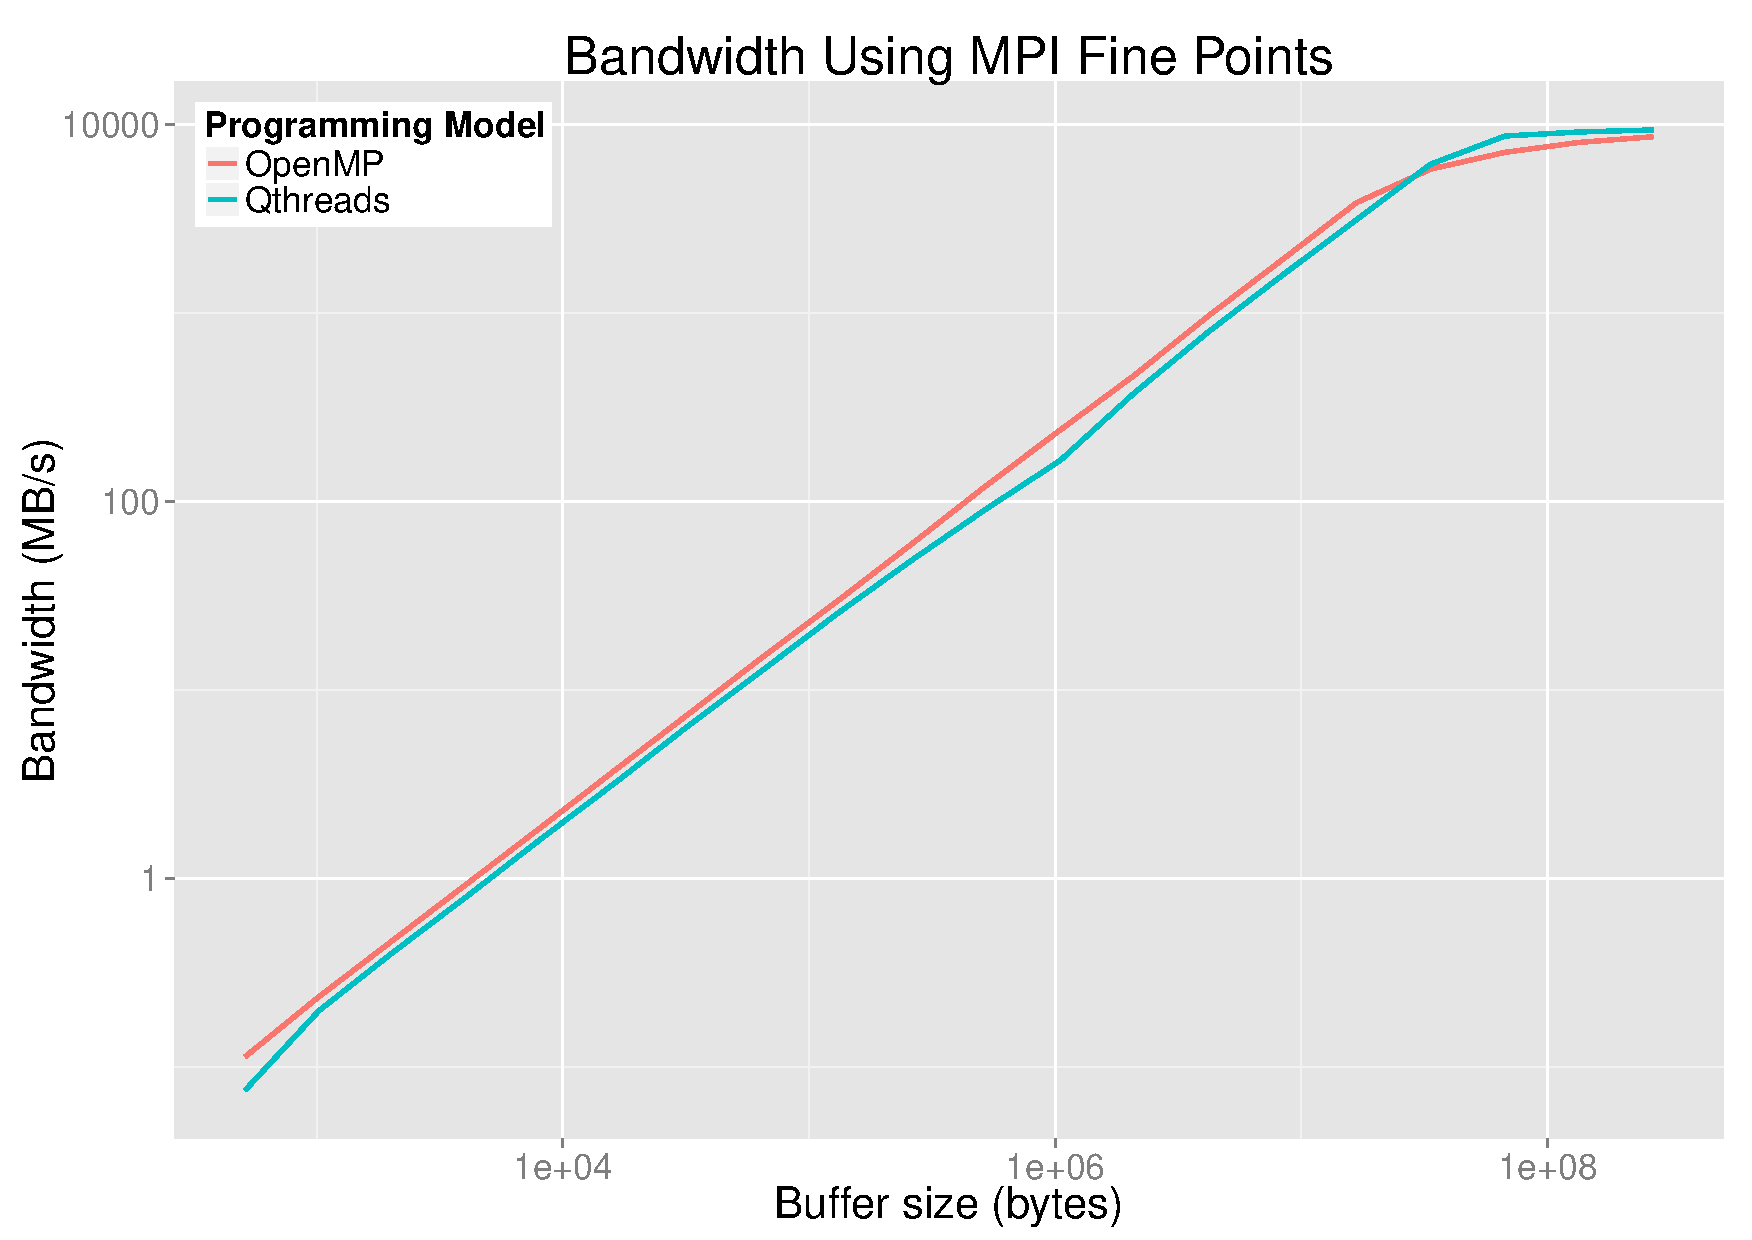
\includegraphics[width=6in]{projects/2.3.1-PMR/2.3.1.15-Qthreads/FinePointsBW-QtOmp.pdf}
	\caption{\label{fig:qthreads-finepoints-graph}This graph shows the performance of Qthreads and OpenMP paired with the FinePoints library for multithreaded MPI.  The x-axis varies the buffer sizes transferred in each experiment in the series, and the y-axis shows the network bandwidth achieved.  The similar performance of Qthreads and OpenMP justifies use of the former as a suitable proxy for the latter, with the advantage of flexibility for rapid prototyping of new runtime system techniques.}
\end{figure}


\paragraph{Next Steps}

We will investigate several possible optimizations, either in terms of Qthreads runtime improvements alone, or in conjunction with the OpenMPI implementation in which Finepoints is natively available as an extension:

\begin{itemize}
\item Enabling the swapping of schedulers in the Qthreads runtime at execution time in response to the tasks set observed.  (Currently the scheduler must be selected at configure time, so we would progress from there to selection at the start of an execution, and finally to a dynamic selection during the execution.)
\item To better enable the coordination of Qthreads and OpenMPI, add Qthreads as an MPI threading model instead of the default pthreads. (This requires modifying OpenMPI's “opal” subsystem to use a new threading mechanism.)
\item To explore this scheduling infrastructure, implement novel scheduling points (e.g. synchronization points in critical regions) allowing contended OpenMPI synchronization areas to schedule Qthreads events and vice versa.
\item With hierarchical and differential scheduling infrastructure in place, seek to design scheduling policies which optimize the interaction between composed runtimes.
\end{itemize}

We anticipate that due to technical and logistical constraints, only a subset of these tasks may be possible, but there will be value in at least attempting them and documenting our findings.  We feel confident that through this work, significant strides will be made toward better coupling of threading and communication.


\newpage
\subsubsection{\stid{1.16} SICM}
\paragraph{Overview} The goal of this project is to create a universal interface for discovering, managing and sharing within complex memory hierarchies. The result will be a memory API and a software library which implements it. These will allow operating system, runtime and application developers and vendors to access emerging memory technologies. The impact of the project will be immediate and potentially wide reaching, as developers in all areas are struggling to add support for the new memory technologies, each of which offers their own programming interface. The problem we are addressing is how to program the deluge of existing and emerging complex memory technologies on HPC systems. This includes the MCDRAM (on Intel Knights Landing), NV-DIMM, PCI-E NVM, SATA NVM, 3D stacked memory, PCM, memristor, and 3Dxpoint. Also, near node technologies, such as PCI-switch accessible memory or network attached memories, have been proposed in exascale memory designs. Current practice depends on ad hoc solutions rather than a uniform API that provides the needed specificity and portability. This approach is already insufficient and future memory technologies will only exacerbate the problem by adding additional proprietary APIs. Our solution is to provide a unified two-tier node-level complex memory API. The target for the low-level interface are system and runtime developers, as well as expert application developers that prefer full control of what memory types the application is using. The high-level interface is designed for application developers who would rather define coarser-level constraints on the types of memories the application needs and leave out the details of the memory management. The low-level interface is primarily an engineering and implementation project. The solution it provides is urgently needed by the HPC community; as developers work independently to support these novel memory technologies, time and effort is wasted on redundant solutions and overlapping implementations. Adoption of the software is focused on absorbtion into existing open source projects such as hwloc, Umpire, CLANG/LLVM, OpenMP, and Jemalloc.
\begin{itemize}
\item  Low-Level Interface: Finished refactor of low-level interface supporting memory arenas on different memory types. Added initial support for Umpire, OpenMP. Reviewing features need to fully support these runtimes. SICM now supports Intel Optane memory, the first NVM memory that can be used as an extension of traditional DRAM memory.
Pull requests have been developed for OpenMP/CLANG/LLVM and Umpire. the patches to Clang/LLVM/OpenMP turn OpenMP memory spaces in OpenMP 5.x into SICM library calls in the LLVM/OpenMP runtime. The same codepath that supports memkind library was refactored to support multiple custom memory allocators – more general than just SICM support.
SICM currently supports "pragma openmp allocate" with  memory types: omp_ (default, large_cap, const, high_bw, low_lat ) _mem_spaces and supports KNL, Optane, testing on Sierra/Summit.

\begin{itemize}
\item  High-Level Graph Interface: Metall is a persistent memory allocator designed to provide developers with an API to allocate custom C++ data structures in both block-storage and byte- addressable persistent memories (e.g., NVMe and Intel Optane DC Persistent Memory) beyond a single process lifetime. Metall relies on a file-backed mmap mechanism to map a file in a filesystem into the virtual memory of an application, allowing the application to access the mapped region as if it were regular memory which can be larger than the physical main-memory of the system.
\item Analysis: 
SICM has employed application profiling and analysis to direct data management across complex memory hierarchy, the team extended the SICM high-level interface with application-directed data tiering based on the MemBrain approach which is more effective than an unguided first touch policy.  The impact of using different data features to steer hot program data into capacity-constrained device tiers was modeled.
\end{itemize}
\paragraph{Next Steps}
\begin{itemize}
\item  Low-Level Interface: Focus on performance of support for runtimes and adding feature requested to support Umpire, OpenMP and MPI and address the slow move pages implementation in the Linux kernel – (collaboration with RIKEN). Test with proxy applications for functionality and correctness. Investigate Linux kernel modifications for page migration in collaboration with ECP project Argo 2.3.5.05 and RIKEN research center in Japan, on-going. Start collaborating with applications to enable use of heterogenous memory on ECP target platforms. Additionally, the team needs to finalize the memory topology discover with the hwloc team.
\item For the analysis work the team will extend and hardend the tools for guiding application memory management and investigate feature categories to classify objects associated with different features such as size, type, allocation time, etc to guide data placement.
\item For the Metall high-level interface we plan to continue outreach to ExaGraph to store graph data as well as other intermediate data into PM leveraging Metall. We also plan to support UMap (user-level mmap library in Argo PowerSteering project) underneath Metall to enhance its performance and capability.
\end{itemize}



\newpage

\subsection{\tools}
This section present projects in \tools.
\newpage
\subsubsection{\stid{2.01} \tools\ Software Development Kits} 

\paragraph{Overview} 
The \tools\ SDK effort is focused on identifying meaningful aggregations of products in this technical area.  SDK efforts are in the early stages of planning and execution.  Most of the work on SDKs has been driven from the \ecosystem\ technical area.  A description of the SDK effort can be found in Section~\ref{subsubsect:ecosystem-sdk}.

\newpage
\subsubsection{\stid{2.02} LANL ATDM Tools}

\paragraph{Overview}
The Los Alamos National Laboratory ATDM Tools project provides tools
and software infrastructure for improving various aspects of the
Exascale programming environment.  At present our efforts are
primarily focused on an advanced LLVM~\cite{LLVM:2018} compiler and
tool infrastructure supporting a new explicit parallel intermediate
representation for the C/C++ and Fortran programming languages.  These
efforts also include interactions with the broader LLVM community and
several platform vendors (e.g. NVIDIA and ARM).  This work also covers
a set of interactions and engagements focused on collaboration with the
Flang project (ST 2.3.5.06) with a goal of providing a long-term Fortran
language capability within the LLVM infrastructure. 

\paragraph{Key Challenges}
One fundamental challenge for our efforts is planning for and
providing system architectures that yet to be completed defined in a
manner that makes them a well-defined target for compilation.  This
risk is likely significantly mitigated given the wide use and adoption
of LLVM across the many key system and processor vendors.  Additional
challenges stem from the adoption of our designs and implementations
into the overall LLVM community -- given their broader and more
general focus.  

\paragraph{Solution Strategy}
Given the project challenges, our approach considers aspects of
today's node-level programming systems (e.g. OpenMP and Kokkos) and
popular programming languages (e.g. C++ and Fortran) into
consideration and aims to improve and expand upon their capabilities
to address the needs of ECP.  This allows us to attempt to strike a
balance between incremental improvements to existing infrastructure
along with more aggressive techniques that seeks to provide innovative
solutions to help both manage risk and the ability to introduce new
breakthrough technologies.

To mitigate some aspects of risk, we are working to form close working
relationships with the LLVM community to help provide an impact and
longer term set of technologies to the broader computing community.
These activities span both academic and industry collaborations.

\paragraph{Recent Progress}
Our most recent efforts have focused on supporting an infrastructure
that maps multiple language constructs from Kokkos, FleCSI and OpenMP
into an common intermediate representation that explicitly captures
the parallel operations for analysis and optimization (this is a
capability that does not exist in the mainline LLVM infrastructure).
This parallel representation may then also be targeted to different
runtime systems (not necessarily those of use by the programming
system used in the original source programs).  See our most recent
paper for a discussion of our overall approach~\cite{Stelle:2017}.  In
addition, this work will be presented at the upcoming EuroLLVM
workshop~\cite{EuroLLVM:2018}.  We will continue to reach out to the
broader LLVM community via such events to provide updates and share the
lessons learned and example use cases of this technology.  Most recently,
at the US LLVM Developer's Meeting, an RFC for was released for
adding parallel intrinsics to LLVM as a collaboration between LANL,
MIT, ANL, Intel, and UIUC~\cite{LLVMPAR:rfc}.

In addition to runtime improvements, we've shown that by compiling
directly to parallel IR instead of the codepath based on C++
template explansion for Kokkos we can gain significant improvements in
overall application compile time and a significant reduction in binary
size. See Figure~\ref{fig:2.3.2.02:time_size} for quantification of the compile
time speedup and binary size reduction.

\begin{figure}
  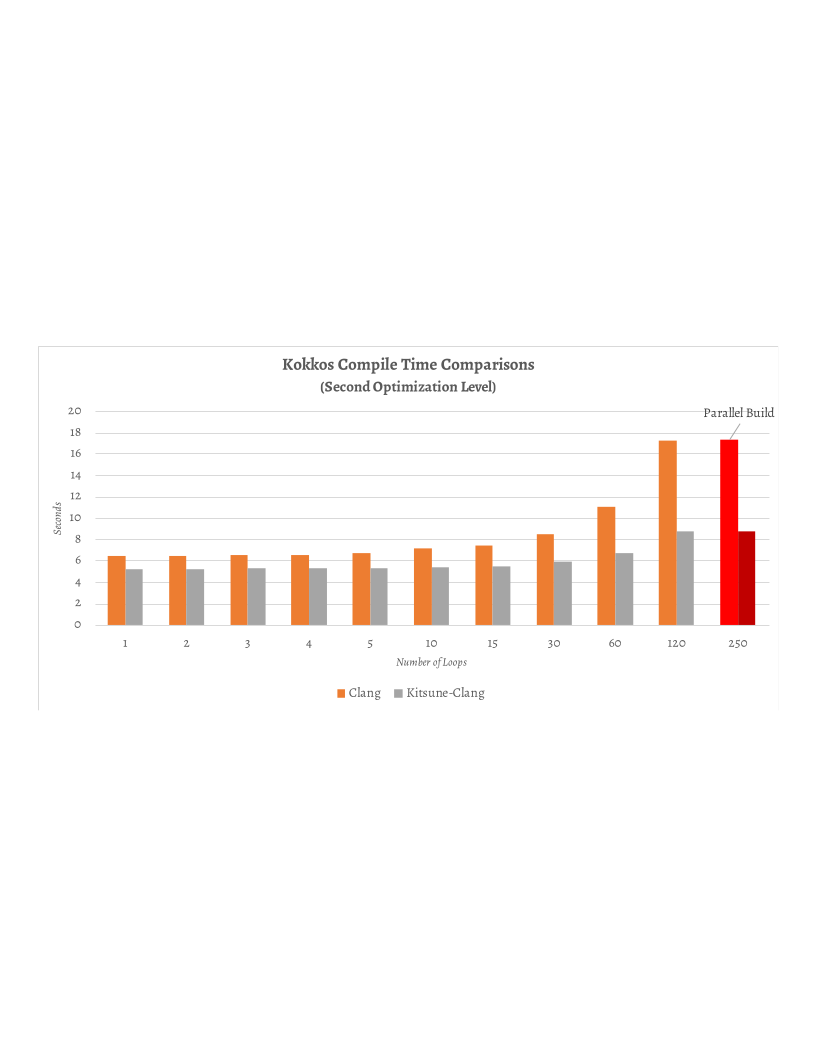
\includegraphics[0.8\textwidth]{projects/2.3.2-Tools/2.3.2.02-LANL-ATDM-Tools/kokkos-compile-times.png}
  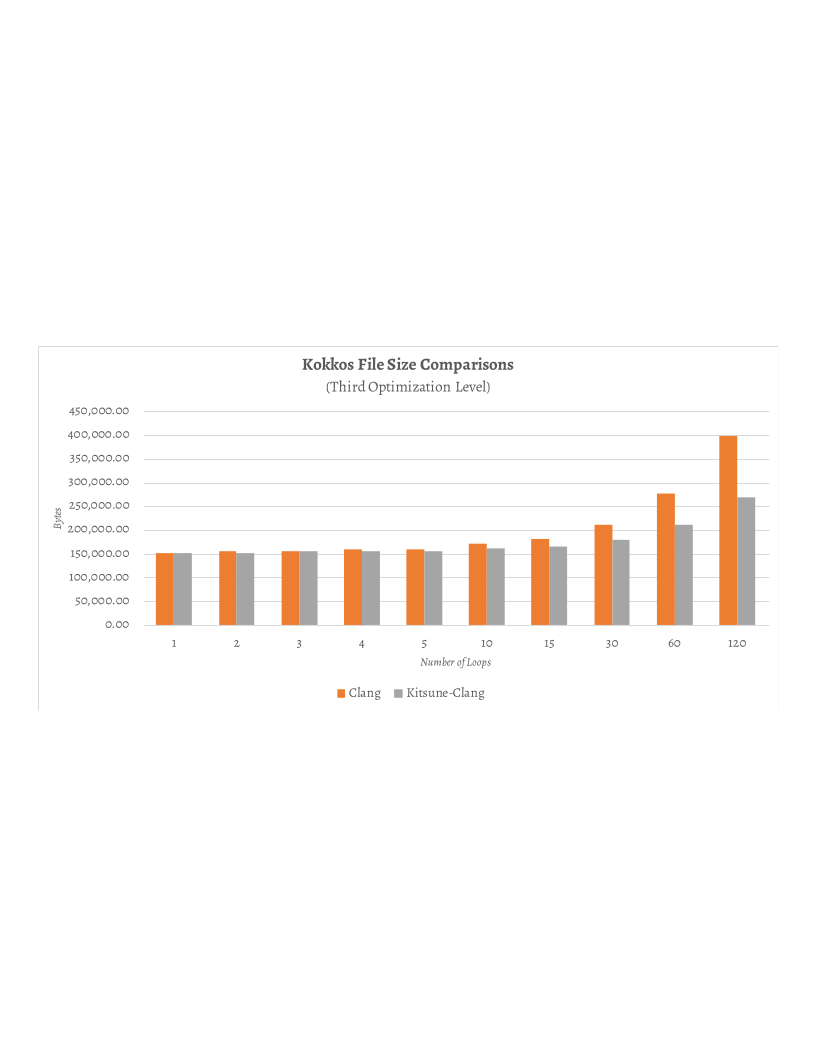
\includegraphics[0.8\textwidth]{projects/2.3.2-Tools/2.3.2.02-LANL-ATDM-Tools/kokkos-file-size.png}
  \caption{Compile time improvements and object file size reductions for
           Kokkos applications with an increasing number of parallel-for
           looping constructs.}
  \label{fig:2.3.2.02:time_size}                      
\end{figure}


\paragraph{Next Steps}
The Kitsune efforts are highlighed by a series of quarterly milestones
and associated software releases throughout the coming year.  The
Kitsune compiler is still very much an active \emph{proof-of-concept}
compiler toolchain focused on C and C++ with plans to soon add support
for Fortran via the Flang project~\cite{Flang:2018}.  Even though it
is not yet production ready we are actively releasing source code and
the supporting infrastructure for deployment as an exploratory and
early evaluation candidate.  These efforts will all continue to
include significant interactions and collaborations with the other ECP
efforts surrounding LLVM and also engage with the broader LLVM and
vendor communities on our assocaited technology.

\newpage
\subsubsection{LLNL ATDM Development Tools Projects}

\paragraph{Overview} The LLNL ATDM Tools Project came together from two tool efforts at LLNL, ProTools and AID.  The ProTools project provides a productization path for research-quality tool software.  The ProTools team works with tool research groups and provides the software engineering effort needed to move their tools into production.  This includes tasks like writing test suites and documentation, porting to new systems, adding user-driven features, and integrating tools with application codes.  Some of the larger efforts in ProTools are:

\begin{itemize}
\itemsep 0em 
\item Ubiquitous Performance Analysis - A suite of tools and visualizations that enable a performance analysis workflow where tools are built into the application and monitor the performance of every run.
\item SCR - The Scalable Checkpoint/Restart library, which abstracts away IO technologies such as burst buffers for applications.
\item mpiFileUtils - A suite of IO-tools based on common UNIX file utilities (cp, rm, cmp, ...), but optimized for HPC.
\item OMPD - A debugging standardization effort for OpenMP.
\item Umpire - An abstraction layer for managing the different types of memory found in current and next-generation systems.
\end{itemize}

The AID project is developing next-generation debugging and code-correctness tools, with a focus towards tool viability at Exascale  The significant projects in AID are:
\begin{itemize}
\itemsep 0em 
\item STAT - A debugging tool that can narrow down the debugging search space for hangs and other issues at massive scales.
\item Archer - A tool for automatically identifying race conditions in OpenMP programs.
\item ReMPI/Ninja - A suite of tools that can inject noise in applications to expose MPI races, and record/replay those races when found.
\item FLiT - A tool for testing floating point consistency and workloads.
\end{itemize}

\paragraph{Key Challenges}
There are several challenging areas that are common not just among the LLNL ATDM Tool Projects, but across tool efforts through-out the HPC community:
\begin{itemize}
\itemsep 0em
\item Platform Portability - Tools are particularly challenging to port to new systems.  Unlike applications, which rely on standards such as OpenMP and MPI, tools are generally built weaker body of standards.  Porting to a new system can involve detailed low-level dives into runtimes and system components.  Tools rarely have platform-independent code bases and require significant effort to bring up on new systems.  
\item Application Complexity - In addition to the increasing complexity of systems, applications are growing in size and complexity.  New programming models are increasing the distance between the low-level machine code that tools generally measure and the high-level code that programmers think about.  Mapping between these layers requires significant infrastructure in each tool.
\item Application Adoption - At any one time it can be easier to add a new printf statement rather than learn a new debugging or performance analysis tool.  It has been historically difficult to encourage application teams to consider tool adoption a priority, though with approaching challenges of next-generation and Exascale system this trend seems to be changing.
\end{itemize}

\paragraph{Solution Strategy}
Specific solutions to the above problems can vary with each instance and tool.  Though there are several high-level trends across the LLNL ATDM Tool Projects:
\begin{itemize}
\itemsep 0em
\item Application and Tool Integration - As previously mention, tools can be challenging because they generally live in a smaller standards space.  Some efforts are towards shifting tools into the application domain, where they can utilize application-level standards and infrastructure.  Examples of this from the Ubiquitous Performance Analysis project and Caliper projects include doing performance attribution with application-level annotations rather than binary analysis and DWARF line mappings.  Or instead of building low-impact tool communication infrastructure like MRNet, we can use MPI have the application team to annotate code with safe communication points.
\item Standardization and Co-design - The LLNL ATDM Tool Project is engaging with standards committees to create tool-specific interfaces in programming models.  The recent OMPD work added a interface for debuggers into OpenMP, which looks likely to be accepted into OpenMP 5.0.  Beyond formal standardization efforts, the LLNL ATDM Tool Projects also work with vendors during system design to ensure the available of tools on upcoming systems.  Team members have recently engaged in the CORAL project and are working directly with IBM and NVIDIA on providing numerous tools.
\item Tool Componentization and Composability - Rather than have tools reinvent the wheel and then stumble over the same potholes in every system, the LLNL ATDM Tool Projects have striven to make tools that both share common best-practice components and be composedly with other tools.  Gotcha, from the Ubiquitous Performance Analysis project, is a new component library that does function wrapping and is being adopted in several other tools.  The AID project is building an inter-operable software stack of debugging tools, where projects like STAT and ReMPI can work together with classical debuggers like TotalView and DDT.  By sharing code and relying on other tool's strengths we can minimize the amount of repeated work across the tools community.
\item Application Adoption - To help application teams adopt tools, members of the LLNL ATDM Tool Projects work directly with them through early tool efforts.  This can take the form of software development effort, such as when ProTools team members helped an ASC application adopt SCR.  Or it can be a hand-holding exercise when first running a tool, such as when the AID team helped a math library identify a significant race condition with Archer.
\end{itemize}


\paragraph{Recent Progress}

There are several recent notable achievements from the LLNL ATDM Tools Projects:
\begin{itemize}
\itemsep 0em
\item The OMPD standard looks likely to be adopted into the OpenMP 5.0 standard.  In addition to the many OpenMP contributors, The ProTools team worked with the standards group in the LLNL ATDM Data and Visualization project on this.  ProTools focused on the reference implementation and the standards group on the standards document.
\item The ProTools team will soon be releasing the initial version of the Gotcha library, which will provide other tools (primarily performance analysis tools) with a better way to implement and control function wrapping.
\item The AID project has had several publication on OpenMP race detection\cite{pmodelconcurrency2018},\cite{swordopenmp2018} and floating point consistency\cite{Flit2017}.
\end{itemize}

\paragraph{Next Steps}

The ProTools team is starting a major new thrust in the Ubiquitous Performance Analysis effort.  They are aiming to add Caliper into a targeted ASC code, and then build and integrated performance analysis workflow that brings together caliper and web-based performance visualization.  The end result of this is to have application users running codes, producing behind-the-scenes performance data, and then application developers browsing and analyzing the performance data with analytic frameworks and novel visualizations.

The AID team is focusing on vendor interactions and co-design, for both CORAL systems and subsequent next-generation systems.


\newpage
\subsubsection{\stid{2.04} SNL ATDM Tools} 

\paragraph{Overview}

The SNL ATDM Tools project is broken into two subprojects: the SNL ATDM DevOps subproject, and the Sandia ATDM Performance Analysis subproject.

The SNL ATDM DevOps subproject focus is on tools and processes supporting development operations (``DevOps'') for the ATDM software development efforts.
DevOps in the SNL ATDM context is all of the software infrastructure development, testing support, integration, and deployment work in support of the ATDM software application and component development teams.

The primary activities of this subproject are to (1) coordinate and prioritize tasks for the various teams that provide DevOps support for ATDM codes, applications, and customers, (2) develop and help deploy shared build, test, and install infrastructure across the ATDM codes and projects, (3) define and support development, testing, integration, and other related workflows for ATDM projects.

The SNL ATDM Performance Analysis subproject is scoped with providing a broad cross-section of portability and performance-related support activities for the laboratories ATDM efforts.
These activities include: (1) providing support for high-performance, hardware-optimized cross-platform builds, including the generation of correct hardware compiler options/software defines; (2) performance
analysis of benchmarking runs, including thread and node scaling on relevant NNSA/ASC testbeds and platforms, and (3) provision for algorithm/code modification or editing of run scripts to optimize performance where issues are identified.

The SNL ATDM Performance Analysis subproject also develops profiling and correctness tools which work with the Kokkos Profiling hooks API.
These tools have been developed to provide insight into the timing of kernels written using Kokkos, as well as data structures utilizing Kokkos parallel containers or Views.
In a number of cases, the profiling tools act as {\em connectors}, establishing a link between important Kokkos performance events and vendor provided tools such as Intel's VTune, NVIDIA's NSight and Arm's MAP profilers.

\paragraph{Key Challenges}

The key challenges associated with this project are the extremely aggressive porting and optimization requirements associated with Sandia's ATDM efforts.
These activities are attempting to port and help support a minimum of three production-class NNSA applications, as well as multiple mini-applications and research prototypes to several ASC-relevant platforms. The first-of-a-kind algorithms being used on these platforms produce complex interactions in the applications that must be fully studied and analyzed to ensure a high level of performance is being offered to the Sandia's user base.

Combined with the application development effort, Sandia is investing heavily in the development of the Trilinos scalable solver stack (used by several codes in ECP and the broader HPC community). The Performance Analysis activity within ATDM is also providing low-level kernel and runtime optimization insight to developers in the Kokkos and Trilinos projects. The DevOps activity within SNL ATDM is providing configuration, build, testing, and workflows tools and processes to keep this stack of software working on the variety of platforms and configurations.

\paragraph{Solution Strategy}

The SNL ATDM Tools has the following primary thrusts:

\begin{enumerate}

\item \textbf{Common Build, Test, and Integration Tools} ensure scalable DevOps efforts and support.

\item \textbf{Testing and Integration Workflows} ensure smooth and productive development and deployment efforts for ATDM software on target platforms.

\item \textbf{High-Performance Applications} ensure well optimized application, library and kernel performance across ASC-relevant computing architectures.

\item \textbf{Performance Portability} ensures performance portability of Sandia ATDM codes across diverse ASC-relevant computing architectures.

\item \textbf{Lightweight Performance Tool Infrastructure} ensures that lightweight tools exist for rapid performance analysis or performance issue identification.

\end{enumerate}

\noindent
The Sandia Performance Analysis sub project was formed from the older Performance Modeling and Analysis Team in 2015.
It's scope was refined to focus specifically on supporting application development activities at the laboratories, with the intent to help provide much stronger levels of performance across the Sandia software portfolio.
The project has provided significant application support since 2015 on topics including application porting and scaling on the ASC Trinity platform, porting to the ASC CTS-1 commodity clusters and has most recently been providing support for the ASC Sierra platform operated by LLNL.

The Kokkos Profiling tools collection was formed in 2015 resulting from research efforts in several successful LDRD projects.
The experimental interface to Kokkos was prototyped in 2014/5 and has since been the default configuration when compiling the Kokkos library.

\paragraph{Recent Progress}

For FY18, the SNL ATDM Tools project has completed the following activities:

\begin{itemize}
\item {\bf Development of Continuous Integration Testing for ASC Platforms} - the DevOps subproject has established a robust, continuous integration suite of tests which are performed over ATS1 (Trinity, Haswell and KNL), ATS2 (CORAL, POWER9/Volta GPU) and ASC CTS1 (Broadwell) systems. These are required platforms for the ATDM code bases. In addition, the subproject has made significant progress on continuous integration pre-merge testing on all of these platforms which will significantly improve code base robustness.

\item {\bf Identification of Testing Performance Issues} - collaboration between the DevOps and tools subprojects has identified an area of potential concern - slow parallel test performance. These occur when the testing infrastructure (CTest) does not have hardware topology/performance awareness and schedules too many tests to use the same resources. Several potential fixes have been investigated and a set of solutions are in prototype form. During FY19, the SNL ATDM project will work to integrate these solutions back into the the CTest testing infrastructure.

\item {\bf Performance Analysis Support} - the performance subproject has continued to provide performance analysis capabilities to ATDM customers, migrating some of its analysis capabilities to include ATS2 (CORAL) and Arm (Vanguard/Astra) platforms in preparation for significant code runs on these machines.
\end{itemize}

\paragraph{Next Steps}

Our next efforts are:

\begin{enumerate}

\item {\bf Evaluation of Spack for Third Party Dependencies} - the DevOps project will work to evaluate Spack as a mechanism for Trilinos third party library build/support.

\item \textbf{Transition ATDM APPs to use unified ATDM Trilinos configurations} - the DevOps project is already well underway with developing unified confgurations for SPARC and EMPIRE which will reduce duplicated work and make more efficient use of build systems.

\item \textbf{Additional Benchmarking:} additional platforms and more extensive benchmarking activities are currently underway, particularly on CORAL POWER9/Volta and Arm-based systems. These studies will have improve the ``day-one'' performance of Sandia's application portfolio on the pre-Exascale ATS platforms when they are released to users for production campaigns in 2019.

\end{enumerate}

%\newpage
%
\subsubsection{Exascale Code Generation Toolkit} 


\paragraph{Overview} 

Our project addresses the development of HPC software for exascale and similarly complex architectures. 
Generated code 
may be modified, wrapped in application specific APIs, or be checked into the user’s application 
repository. Inputs to the code generation tools we have developed are either application 
code or simplified application code that represents naive implementations of algorithms. Input languages 
we are supporting include both legacy and modern versions of Fortran, C, and C++ 
(e.g., F77, F2008, F2015, C89, C99, C11, C++98, C++11, C++14, C++17, etc.). The output is generated 
code in the same language, but modified to address essential hardware-specific architectural features. 
We are supporting common language dialects including: UPC, OpenMP 
(for both C, C++, and Fortran), CUDA, and OpenCL.

\paragraph{Key  Challenges}

   Our project addresses the development of HPC software for exascale and
similarly complex architectures.
The approach in our project supports only the generation of code to simplify 
the job of the developers, and as such 
users are given complete control over how to use our code generation tools.
However, this makes our project especially difficult because we must read and rewrite 
the user's source code application.  This step requires significant compiler technology: 
analysis and transformations at the source code level so that it can leverage the vendor's compiler.
% Generated code may be modified, wrapped in application specific APIs, or be checked 
% into the user's application repository. 

We operate using a source-to-source approach so that the target architecture's compiler 
(vendor compiler) may be used to full advantage. It is expected that the vendor's compiler 
will be best optimized (low level optimizations) to the vendor's architecture. However, 
the structure of code written (at a high level) to take advantage of the vendor compiler's 
optimization can be exceedingly complex, vary widely between vendors, and is thus well 
better suited to automated code generation.

\paragraph{Solution Strategy}


Figure~\ref{fig:2.3.2.05-ExascaleCodeGenToolkit} illustrates the approach used to process 
application code and automate transformations to support either performance optimization 
or correctness checking.
\begin{figure}[htb]
	\centering
	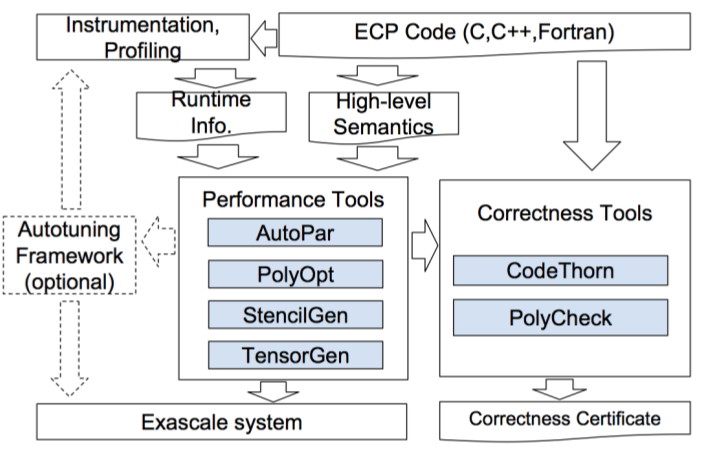
\includegraphics[width=4.5in]{projects/2.3.2-Tools/2.3.2.05-Exascale-Code-Generation-Toolkit/ExascaleCodeGenToolkit.png}
	\caption{\label{fig:2.3.2.05-ExascaleCodeGenToolkit} Approach to processing user application 
                 code with multiple tools to support optimization and correctness checking.}
\end{figure}
Our project is developing several tools for generating code: PolyOpt (a polyhedral 
optimizations program transformation engine capable of fully automating highly complex loop transformations), 
AutoPar (an automatic parallelization tool that inserts OpenMP directives into serial codes), 
CodeThorn (an award winning code correctness tool built using ROSE and SPOT),  PolyCheck (a code 
correctness tool specific to polyhedral optimizations), and ROSE (a widely used compiler infrastructure 
for building specialized compiler tools). Our tools allow users to easily specify portions of an input application and 
automatically generate semantically equivalent, but higher performing code variants; including the ability 
to generate a multiple variants that traverse a space of optimizations (e.g., loop tiling sizes, loop fusion, 
loop fission alternatives, etc.). The PolyOpt polyhedral optimizer is being enhanced with pattern-specific 
optimization and code generation strategies to address important patterns found in ECP codes. Stand-alone 
code generators developed previously by us for stencil computations and tensor contractions are being 
integrated with PolyOpt and their capabilities enhanced and hardened (StencilGen and TensorGen).  The 
use of CodeThorn and PolyCheck have already been demonstrated for the verification of correctness of 
such automatically generated code.

\paragraph{Recent Progress}

We have made a release of TensorGen to the NWChem team and it has been used in their NWChem production 
release this past Fall (Fall 2017).

The StencilGen code generator takes as input a DSL specification of stencil functions and their domains, and 
creates CUDA code from it. The tool employs fusion, streaming, and overlapped tiling to achieve high performance. 
In order to avoid register spills for complex stencils, the tool also performs statement reordering that takes as 
input straight-line CUDA code for a multi-statement stencil and models it as a DAG of expression trees. The 
statements are then reordered to minimize register pressure \cite{PPoPP18}.

The AutoPar tool accepts C/C++ serial programs as input and automatically generates OpenMP loop directives. We 
have continued to work on the CPU cost model to guide AutoPar’s automatic parallelization. We have created a model 
based on the roofline model, and an existing tool in ROSE (the Arithmetic intensity tool) has been improved to 
provide key information for our model. We also added one option to use inlining in order to support loops with 
simple C function calls.  Several microbenchmarks, including EPCC and STREAM, have been investigated and used 
to extract hardware and software metrics needed in our model.

CodeThorn takes as input polyhedral parallelized loops generated by the tool PolyOpt and checks whether the 
optimized loops are equivalent to the original (non-optimized) loops. We analyzed the availability of optimizable 
code patterns for verification in three proxy apps (AMG2013, CoMD, LULESH) and found 282 optimizable patterns 
that can serve as input to our verification. We extended the scope of the covered C++ subset for verification 
to support changes in the PolyOpt generated optimized code. We also extended the representation of program states 
to take pointers to dynamic data structures into account.

We have been developing the other tools mentioned above, adding supporting features, and testing to them.
We gave a demo of these tools at the recent ECP all-hands meeting in February, 2018; and we distribute 
the working versions of these tools that we demonstrated at the meeting.  These tools are regularly updated 
with ongoing work and released as part of Continuous Integration (CI) processes.  Most tools are released
as part of the ROSE distribution to simplify the testing and release process.

We have been adding new Fortran support to ROSE as part of our ECP Fortran support. We have also started 
the C++17 support in ROSE. We have compiled most of the ECP proxy applications as part of initial first 
year work. We now test the ROSE C and C++ compiler infrastructure against commercial compiler tests suits
and it performs similarly to commercial compilers in initial testing for analysis tools.



\paragraph{Next Steps}

For StencilGen, we will develop several heuristics for fusion, streaming, and tiling based on architectural 
characteristics, as well as machinery to systematically explore various compositions of optimizations and 
optimization parameters. We will continue to work with the NWChem team at PNNL to support their computational 
code generation requirements.
For CodeThorn we will (i) extend the evaluation with proxy apps and (ii) improve the reporting of detected 
semantic differences in the PolyOpt optimized code in comparison to the original code.

We are also working with the AMReX ECP team to support analysis and transformation of their application codes
using our tools and future versions of them with additional features.  The AMReX team is in turn also 
supporting multiple ECP application teams, to which all of our work is expected to apply directly.


 


\newpage
%\subsubsection{\stid{2.06} Exa-PAPI++}\label{subsubsect:exapapi}

\paragraph{Overview} 

%Understanding the performance characteristics of exascale applications is 
%necessary in order to identify and address the barriers to achieving performance 
%goals. This becomes more difficult as the architectures become more complex. 
%The Performance Application Programming Interface (PAPI) provides both library 
%and application developers with generic and portable access to low-level 
%performance counters found across the exascale machine, enabling users to see
%the relationships between software performance and hardware events. 
%These relationships provide a critical step toward improving performance.

The Exa-PAPI++ 
project is developing a new C++ Performance API (PAPI++) software package 
from the ground up that offers a standard interface and methodology for using
low-level performance counters in CPUs, GPUs, on/off-chip memory, interconnects, 
and the I/O system, including energy/power management. 
PAPI++ is building upon classic-PAPI functionality and strengthening its path to
exascale with a more efficient and flexible software design, one that takes 
advantage of C++'s object-oriented nature but preserves the low-overhead 
monitoring of performance counters and adds a vast testing suite.

In addition to providing hardware counter-based information, a standardizing layer 
for monitoring software-defined events (SDE) is being incorporated that exposes 
the internal behavior of runtime systems and libraries, such as communication and 
math libraries, to the applications. As a result, the notion of performance events is 
broadened from strictly hardware-related events to include software-based 
information. Enabling monitoring of both hardware and software events provides 
more flexibility to developers when capturing performance information.


\paragraph{Key Challenges}

Widely deployed and widely used, PAPI has established itself as fundamental
software infrastructure in every application domain where improving performance
can be mission critical. 
However, processor and system designs have been experiencing radical changes.
Systems now combine multi-core CPUs and accelerators, shared and
distributed memory, PCI-express and other interconnects, and
power efficiency is emerging as a primary design constraint.
These changes pose new challenges and bring new
opportunities to PAPI. At the same time, the ever-increasing importance of
communication and synchronization costs in parallel applications, as well as the
emergence of task-based programming paradigms, pose
challenges to the development of performance-critical applications and create a
need for standardizing performance events that originate from various ECP
software layers.


\paragraph{Solution Strategy}

The Exa-PAPI++ team is preparing PAPI support to stand up to 
the challenges posed by exascale systems by 
\begin{enumerate}
\item widening its applicability and providing robust support for exascale 
hardware resources;
\item supporting finer-grain measurement and control of power, thus offering 
software developers a basic building block for dynamic application optimization 
under power constraints; 
\item extending PAPI to support software-defined events; and 
\item applying semantic analysis to hardware counters so that the application 
developer can better make sense of the ever-growing list of raw hardware 
performance events that can be measured during execution. 
\end{enumerate}

%The Exa-PAPI effort delivers new PAPI components to handle the wide range of
%new hardware and software events for the extreme scale platforms that will form
%the basis of exascale computing. To achieve this, Exa-PAPI implements a variety
%of monitoring and sampling capabilities for the different technologies, which
%are exported to the ECP application community. 
%%
%Exa-PAPI also provides finer-grain measurement and control of power, thus
%offering software developers a basic building block for dynamic application
%optimization under power constraint. Other hardware efforts in Exa-PAPI are the
%development of components for monitoring network interconnect events, as well as
%components targeted at the deep and heterogeneous memory hierarchies that we
%are already seeing in new architectures.

In summary, the team will be channeling the monitoring capabilities of hardware 
counters, power usage, software-defined events into a robust PAPI++ software 
package. PAPI++ is meant to be PAPI's replacement---with a more flexible and 
sustainable software design.


\paragraph{Recent Progress}

On the \textbf{software event} front, the PAPI team has designed and implemented 
a new API to expose any kind of software-defined events. Since September 2019,
the SDE functionality is publicly available through the main repository of PAPI. 
As a result, software packages that reside in any layer of the software stack can now 
export information to the outside world in a uniform, well supported, and 
standardized way. 
 %
Since the concept of software-defined events is still new to PAPI, the team has worked
closely with developers of different ECP libraries and runtimes that serve as natural targets
for the adoption of the new SDE API.
As of today, we have integrated SDEs into the sparse linear algebra library MAGMA-Sparse 
(2.3.3.13 CLOVER), the tensor algebra library TAMM (2.2.1.02 NWChemEx), 
the task-scheduling runtime PaRSEC (2.3.1.09 PaRSEC), and the compiler-based 
performance analysis tool BYFL (2.4.2 HE). 

%\vspace{-4pt}
\begin{figure}[!h]
\begin{center}
  \subfloat[ ]{\label{fig:sde_magma}
  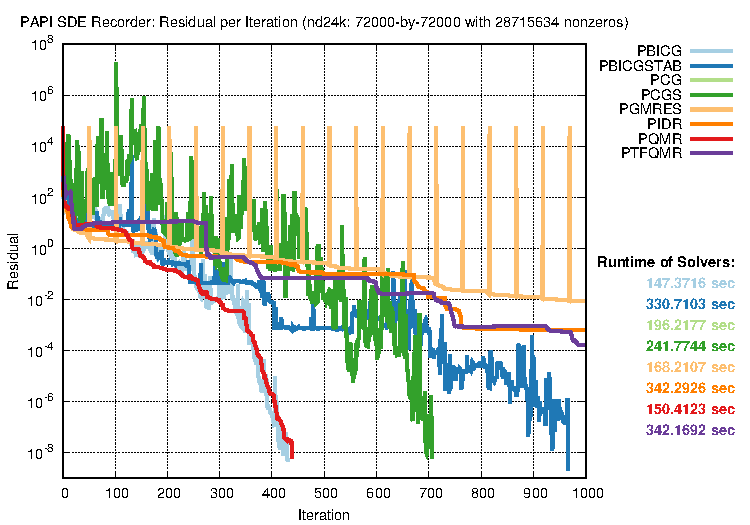
\includegraphics[width=0.49\linewidth]{projects/2.3.2-Tools/2.3.2.06-EXA-PAPI/Exa-PAPI_sde_magma.pdf}}
  \subfloat[ ]{\label{fig:sde_parsec}
  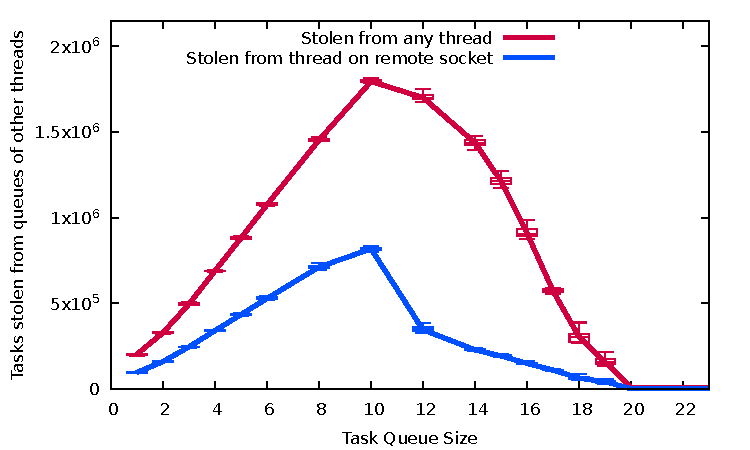
\includegraphics[width=0.49\linewidth]{projects/2.3.2-Tools/2.3.2.06-EXA-PAPI/Exa-PAPI_sde_parsec.pdf}}
%\vspace{-8pt}
\end{center}
\vspace{-9pt}
\caption{(a) PAPI SDE-Recorders log convergence of different ILU-preconditioned MAGMA-sparse Krylov solvers for a 2D/3D Problem; (b) PAPI SDEs count number of times the scheduler stole tasks from the task queue of another thread in PaRSEC.}
\end{figure}
%\vspace{-8pt}
%
%
The examples in Figure~\ref{fig:sde_magma} illustrate how the convergence of Krylov solvers can be
visualized with the help of PAPI SDEs. Each of these solvers behave very differently 
for different problems and matrices, which, once more, stresses the importance of 
\emph{exposing these details in a standardized way}. This allows the domain
scientist to quickly identify the fastest and most robust method of choice for 
their very unique problems. Most importantly, this information can now be obtained without 
expert knowledge about algorithm-specific characteristics,
and without having to instrument MAGMA library code, but simply by calling \verb+PAPI_read()+
in the top-level application.

Figure~\ref{fig:sde_parsec} serves as a second showcase, illustrating the evolution of 
task stealing during the execution of a PaRSEC application that is based on 
fork-join parallelism with 20 tasks generated at each fork.
With SDEs in PARSEC, a user can get a view of what is happening inside the runtime
by simply calling \verb+PAPI_start()+ and \verb+PAPI_stop()+ in their application, without the need to
instrument the PaRSEC runtime code. 


\vspace{10pt}
On the \textbf{hardware counter} front, we have developed support for the latest 
features on NVIDIA Volta GPUs (V100) as featured on the Summit and Sierra systems.
Specifically, PAPI users can now monitor both GPU hardware events and the NVLINK performance. 
Additionally, we developed PAPI capabilities for monitoring power consumption, fan speed, 
temperature, and power capping support for the V100 GPUs. 
The latest version of PAPI (5.7.0, released April 2019) has fully integrated support for the 
NVIDIA GPU counters and power management.
Similar efforts are currently in progress enabling users to monitor performance counters 
as well as power consumption on the AMD Vega GPUs.


\paragraph{Next Steps}

Our next efforts will focus on:
\begin{enumerate}
\item \textbf{Formulation of requirements for new PAPI C++ API:} 
		Create and circulate a survey to the ECP teams to assess their needs for hardware 
		and software performance counter functionality. Based on the survey results, 
		we will determine what features are needed for the new PAPI C++ interface. 
		Furthermore, perform a software requirement analysis, and explore novel concepts 
		for expressing software event and hardware counter 
		monitoring through the same PAPI C++ interface.
%
\item \textbf{Decompose PAPI's SDE functionality as standalone library}: 
		The SDE functionality will be decomposed from the PAPI package and made 
		available as a separate library. The production-ready version of the PAPI SDE 
		library will have fully integrated support for enabling SDEs in ECP software
		layers, as well as monitoring these new events through the PAPI interfaces.
%
\item \textbf{Formulation of a roadmap for refactoring traditional PAPI to PAPI++ software package}:
		Start the PAPI++ design process 
		for a modular framework that includes a new C++ API in addition to the traditional C 
		and Fortran APIs to preserve backward-compatibility. This effort involves a managed 
		transition away from our legacy PAPI software while continuing to add support for new 
		ECP hardware (released during FY20-21) until the official release of PAPI++.
\end{enumerate}

\subsubsection{Exa-PAPI}\label{subsubsect:exapapi}

\paragraph{Overview} 

The Exascale Performance Application Programming Interface (Exa-PAPI) project
builds on the widely deployed and widely used Performance API (PAPI) and
extends it with performance counter monitoring capabilities for new and
advanced ECP hardware and software technologies, fine-grained power management
support, and functionality for performance counter analysis at task granularity
for task-based runtime systems. Exa-PAPI also adds events that originate from
the ECP software stack (i.e., communication libraries, math libraries, task
runtime systems, etc.) and, as a result, extends the notion of performance
events from strictly hardware-related ones to include software-based information. 

Exa-PAPI is essential for ECP because it enables the ECP application community
to monitor both types of performance events---hardware- and
software-related---in a uniform way, through one consistent PAPI interface. On
the hardware side, Exa-PAPI provides access to a wide range of new
events for the extreme-scale platforms that will form the basis of exascale
computing. Furthermore, it provides a finer-grain measurement and control of
power, thus offering software developers a basic building block for dynamic
application optimization under power constraint.  In addition to providing
hardware counter based information, Exa-PAPI integrates a standardizing layer
for monitoring software-defined events (SDEs), which will expose the internal behavior
of runtime systems and libraries to the applications. Addressing the gap of
software-defined event monitoring---and enabling monitoring of both types of
performance events though Exa-PAPI---stands to offer a transformative impact on
performance analysis and application development as a whole.


\paragraph{Key Challenges}

Widely deployed and widely used, PAPI has established itself as fundamental
software infrastructure in every application domain where improving performance
can be mission critical. 
However, processor and system designs have been experiencing radical changes.
Systems now combine multi-core CPUs and accelerators, shared and
distributed memory, PCI-express and other interconnects, and
power efficiency is emerging as a primary design constraint.
These changes pose new challenges and bring new
opportunities to PAPI. At the same time, the ever-increasing importance of
communication and synchronization costs in parallel applications, as well as the
emergence of task-based programming paradigms, pose
challenges to the development of performance-critical applications and create a
need for standardizing performance events that originate from various ECP
software layers.


\paragraph{Solution Strategy}

The Exa-PAPI project prepares the PAPI library to stand up to the challenges posed 
by exascale systems by:
(1) widening its applicability and providing robust support for hardware resources that 
are currently out of PAPI's scope;
(2) supporting new programming paradigms, such as task-based systems, by adding 
functionality for performance counter analysis at task granularity (as opposed to core 
and thread granularity); 
(3) extending PAPI to support software-defined events, in addition to the traditional 
hardware-based events; and 
(4) applying semantic analysis to hardware counters so that the application developer 
can better make sense of the ever-growing list of raw hardware performance events 
that can be measured during execution.

The Exa-PAPI effort delivers new PAPI components to handle the wide range of
new hardware and software events for the extreme scale platforms that will form
the basis of exascale computing. To achieve this, Exa-PAPI implements a variety
of monitoring and sampling capabilities for the different technologies, which
are exported to the ECP application community. 
%
Exa-PAPI also provides finer-grain measurement and control of power, thus
offering software developers a basic building block for dynamic application
optimization under power constraint. Other hardware efforts in Exa-PAPI are the
development of components for monitoring network interconnect events, as well as
components targeted at the deep and heterogeneous memory hierarchies that we
are already seeing in new architectures.


\paragraph{Recent Progress}

The Exa-PAPI hardware and power effort began with the implementation of new
PAPI components enabling Intel Knights Landing (KNL) hardware counter and power
management support. In December 2017, the latest version of PAPI (5.6.0) was
shipped, releasing two new components that are fully integrated into the PAPI library for 
KNL core and uncore support. Additionally, PAPI ships with a powercap component for 
power/energy measurement and control. This development delivers two improvements. 
First, in the past, PAPI power components supported only \emph{reading} power information. 
The new component exposes running average power limit (RAPL) functionality to allow users 
to read and write power. Second, the original PAPI power component accessed the RAPL 
model-specific registers (MSRs) directly, and, therefore, reading
power data required root privileges. The new PAPI power component uses the
powercap interface that comes built-in with the Linux kernel. The purpose of this
interface is to expose the RAPL settings to user-space. Therefore, power
reading is possible without any superuser privileges---only Linux kernel version
3.13 (or higher) is required.

Since the concept of writing (or capping) power is new to PAPI, we studied
numerical building blocks of varying computational intensity, and used the PAPI
powercap component to detect power optimization opportunities. We experimented
with a wide range of power caps on the KNL architecture to reduce
the power usage for different numerical kernels while keeping the execution
time constant so that real energy savings can be achieved.
Figure~\ref{fig:Jacobi_power} shows one example where we use
the Jacobi iterative method to solve a finite difference discretization of the
Helmholtz equation. While the default power consumption is around 185 Watts,
with power capping, we were able to improve the energy efficiency by~25\%
without any loss in time-to-solution. All our findings have been published in a
conference paper~\cite{power1} and a journal paper~\cite{power2}.
%
\vspace{-4pt}
\begin{figure}[!h]
\begin{center}
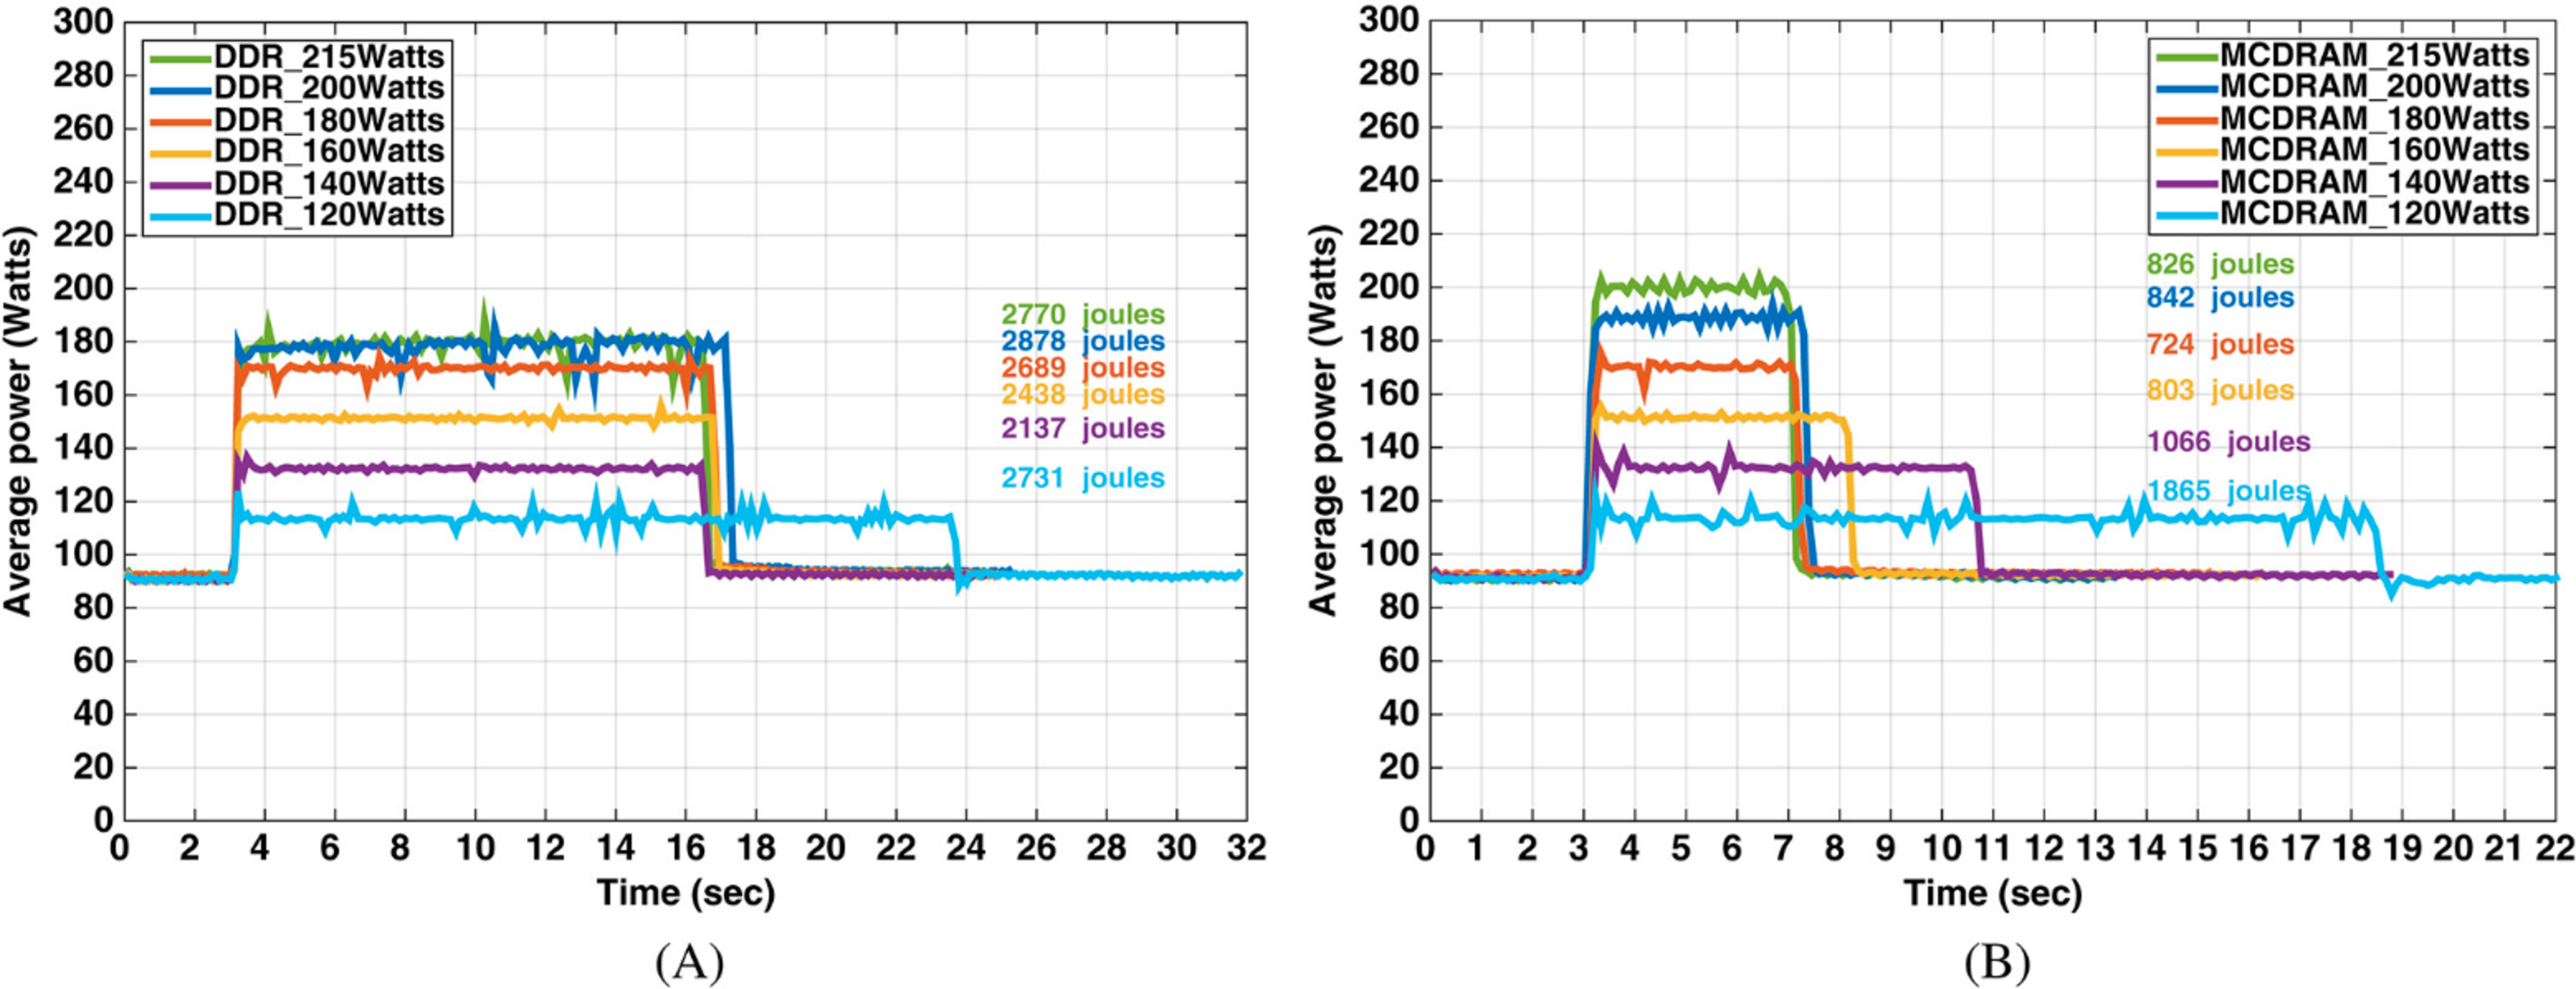
\includegraphics[width=0.82\textwidth]{projects/2.3.2-Tools/2.3.2.06-EXA-PAPI/Exa-PAPI-jacobi.pdf}
\caption{Average power measurements (Watts on y axis) of Jacobi algorithm on a 
12,800 x 12,800 grid for different power caps. (A) FLAT mode: data allocated to DDR4; 
(B) FLAT mode: data allocated to MCDRAM}
\label{fig:Jacobi_power}
\end{center}
\end{figure}
%
\vspace{-8pt}

On the software-defined events front, we have already proposed an API
(publicly available on Jira:
\url{https://jira.exascaleproject.org/secure/attachment/12251/2017_SDE_API_report.pdf})
and received significant feedback and requests for changes by members of the
runtime and library communities, which we have incorporated. We have also
developed a prototype implementation of an SDE component in PAPI, which we are
using to integrate SDE support in various ECP projects, such as:
%
\begin{enumerate}
\vspace{-3pt}
\item ByFL (HT-DSE): \url{https://bitbucket.org/jagode/byfl_papi_sde}
\vspace{-5pt}
\item PaRSEC (2.3.1.09 STPM11-ParSEC): \url{https://bitbucket.org/herault/parsec/branch/PAPI-SDE}
\vspace{-5pt}
\item PEEKS (2.3.3.10 STMS11-PEEKS): \url{https://bitbucket.org/icl/magma} (branch: \verb+PAPI_SDE+)
\vspace{-5pt}
\item NWchemEx (2.2.1.02 ADSE11-NWChemEx): \url{https://bitbucket.org/jagode/nwchem_papi_sde}
\end{enumerate}

\paragraph{Next Steps}

Our next efforts will focus on:
\begin{enumerate}
\item \textbf{Development of a PAPI component for IBM Power9 Hardware Counter
	Support:} Add support for (1) core performance events, which are specific
		to each core; and (2) shared events, which monitor the performance of
		node-wide resources that are shared between cores. Access to shared
		events require elevated privileges. However, IBM's official route for providing
		access to shared events will be through the
		Performance Co-Pilot (PCP) for non-root users. Thus, one of the
		Exa-PAPI efforts is to develop a PAPI-PCP component so that all users
		can access Power9 shared events through PAPI.
%
\item \textbf{Release of PAPI's SDE component, and integration of SDEs with other ECP efforts}: 
		Refine the PAPI SDE prototype implementation based on
		feedback from the ECP community and experience acquired from
		instrumenting ECP projects. Instrument ECP libraries, runtimes, and
		applications, such as PaRSEC, PEEKS, and NWChem to use software-defined
		events to export performance information.
\end{enumerate}

\newpage
\subsubsection{\stid{2.07} YTune} 

\paragraph{Overview}

We are developing tools and an application development workflow that separates a high-level C/C++/FORTRAN implementation from an architecture-specific implementation (OpenMP, CUDA, etc.), optimization, and  tuning.   This  approach
will enable Exascale application  developers to express and  maintain a
single, portable implementation of their computation that is also legal code
that can be compiled and run by using standard tools.   The autotuning compiler
and search framework will transform the baseline code into a   collection of
highly-optimized implementations. This reduces the need for extensive manual tuning.
Both code transformation and autotuning are essential in ECP for providing
performance portability on Exascale platforms.  Due to significant architectural
differences in ECP platforms, attaining performance portability may  require
fundamentally different  implementations of software -- different strategies for
parallelization, loop order,  data layout, and exploiting SIMD/SIMT.  A key
concern of ECP is the high cost of developing  and maintaining
performance-portable applications for  diverse Exascale architectures, including
manycore CPUs and GPUs. 
Ideally Exascale application developers would express their
computation separate from   its mapping to hardware, while autotuning compilers can automate this mapping and achieve performance portability.

\paragraph{Key  Challenges}
Autotuning has the potential to dramatically improve the performance portability of Petascale and Exascale applications.  To date, autotuning has been used primarily in high-performance applications through tunable libraries or previously tuned application code that is integrated directly into the application.
If autotuning is to be widely used in the HPC community,
support for autotuning must address the software engineering challenges, manage configuration overheads, and continue to demonstrate significant performance gains and portability across architectures.
In particular, tools that configure the application must be integrated into the application build process so that tuning can be reapplied as the application and target architectures evolve.

\paragraph{Solution Strategy}
We are developing pluggable software infrastructure that incorporates
autotuning at different levels: compiler optimization, runtime configuration of application-level parameters and system software.
To guarantee success in the ECP time frame, we are collaborating with
application teams, such as SuperLU and QMCPACK, to impact performance of their
codes and libraries.

The autotuning compiler strategy revolves CHiLL, which has the following distinguishing features:
(1) \textit{Composable transformation and code generation}, such
that the same tool can be applied
to multiple different application domains;
(2) \textit{Extensible to new domain-specific transformations} that can be represented as transformations on loop nest iteration spaces are also
composable with existing transformations;
(3) \textit{Optimization strategies and parameters exposed to autotuning:}
By exposing high-level expression
of the autotuning search space as transformation recipes, the compiler writer, an expert programmer or embedded DSL designer can directly \
express how to compose
 transformations that lead to different implementations.
A part of our efforts in ECP are to migrate these capabilities of CHiLL
into the Clang/LLVM open-source compiler, as well as provide lightweight
interfaces through Python, C++, and REST APIs/web services.

For example, we have developed a \textit{brick data layout library and code generator} for
stencil computations within CHiLL.
Recent trends in computer architecture that favor computation over data movement incentivize high-order methods.  Paradoxically, high-order codes can be challenging for compilers/optimization to attain high performance.  Bricks enable high performance and make fine-grained data reuse and memory access information known at compile time.  The SIMD code generation achieves performance portability
for high-order stencils for both CPUs with wide SIMD units (Intel Knights
Landing) and GPUs (NVIDIA Pascall).  Integration with autotuning attains
performance that is close to Roofline performance bound for both manycore CPU
and GPU architectures.

The Search using Random Forests (SuRF) search framework is a separate tool in Y-Tune that optimizes the search over an autotuning search space.  While
SuRF provides support to CHiLL for compiler-directed autotuning, it can
also be integrated directly with applications and runtimes to search over
application parameters and alternative code variants.
SuRF is an asynchronous search framework that consists of sampling a small number of input parameter configurations and progressively fitting a surrogate model over the input-output space until exhausting the user-defined maximum number of evaluations. The framework is designed to operate in the master-worker computational paradigm, where one master node fits the surrogate model and generates promising input configurations and worker nodes perform the computationally expensive evaluations and return the outputs to the master node. We implemented both MPI- and scheduler-based master-worker approaches.


\paragraph{Recent Progress}


We have pursued the following main activities since the beginning of 2018:

\textit{Autotuning capability in LLVM:}
The key idea is to support the use of pragmas in the C++ source to guide transformations to be applied. These can include the types of transformation recipes used in CHiLL, but also parallelization directives for OpenMP and OpenACC that would interact with SOLLVE and PROTEAS. Our initial focus is the implementation of user/tool-directed optimizations in Polly, which is a polyhedral framework in LLVM with some similar features to CHiLL. An initial plan for pragmas in Clang and LLVM metadata has been developed. Several existing open-source LLVM projects allowing for just-in-time (JIT) compilation of C++ code have been identified and are being evaluated for use with autotuning. A summer intern has been identified who will work on the JIT/autotuning explorations.

\vspace*{.1in}
\noindent
\textit{SuRF for SuperLU and QMCPACK:}
We focused on testing and hardening SuRF for tuning SuperLU package. We used 6 matrices that come from different DOE applications and ran SuRF in an asynchronous mode with up to 32 nodes. We compared the results from SuRF to those from OpenTuner. On all instances tested, we found that SuRF obtains comparable results but in half the time of OpenTuner. We also observed that SuRF found high quality solutions in short computation time and used the remaining time for neighborhood exploration. Therefore, we implemented early stopping criterion. We also did single node tuning experiments with QMC. Since the current search space of QMCPACK is rather small, we did not evaluate it at scale. Currently, we are working with the QMCPACK developers to expose more parameters.
Recently, we developed stopping criterion based on local convergence and expected improvement over time. This allows the search to terminate in shorter computation time. Currently, we are expanding the search for multinode autotuning where each evaluation spans multiple nodes.

\vspace*{.1in}
\noindent
\textit{Brick Library:}
We developed a code generator for the Brick Data Layout library for stencils
that is performance-portable across CPU and GPU architectures, and addresses the
needs of modern multi-stencil and high-order stencil computations. The key
components of our approach that lead to performance portability are (1) a
fine-grained brick data layout designed to exploit the inherent multidimensional
spatial locality common to stencil computations; (2) vector code generation that
can either target wide SIMD CPU instructions sets such as AVX-512 and SIMT
threads on GPUs; and, (3) integration with autotuning framework to apply
architecture-specific tuning. For a range of stencil computations, we show that
it achieves high performance for both the Intel Knights Landing (Xeon Phi) CPU,
and the NVIDIA P100 (Pascal) GPU \cite{P3HPC_Bricks}. 

\paragraph{Next Steps}
In the near future, we will release the CHiLL autotuning compiler, and
demonstrate application and library kernel performance gains from 
using the brick data layout.  We will continue the transition of CHiLL capabilities to LLVM.
In SuRF, we plan to explore multinode search, and integrate SuRF into the compiler-directed autotuning we are doing.

\begin{figure}[h]
%\begin{wrapfigure}{r}{0.35\textwidth}                                                                                                     
\begin{center}
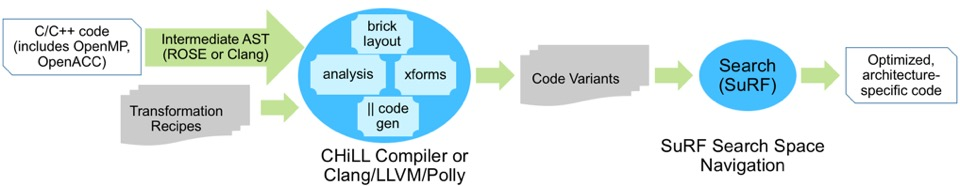
\includegraphics[width=.8\textwidth]{projects/2.3.2-Tools/2.3.2.07-Autotuning/YTune-solution.jpg}
% 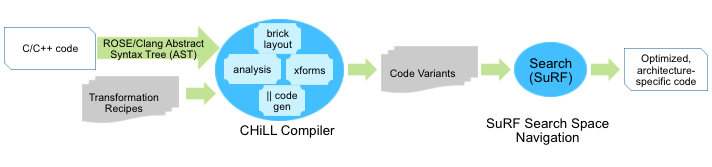
\includegraphics[width=.8\textwidth]{YTune-solution.png}
% \includegraphics[width=.8\textwidth]{PastedGraphic-1.png    }
\end{center}
\caption{Y-TUNE Solution Approach.}
%\caption{S.}                                                                                                                              
%\end{wrapfigure}                                                                                                                          
\end{figure}

\end{document}

\newpage

\subsubsection{\stid{2.08} HPCToolkit} 
\paragraph{Overview} 

The HPCToolkit project is working to develop performance measurement and analysis tools to help ECP software developers understand where and why their programs do not fully exploit hardware resources within and across nodes of extreme-scale parallel systems. Key deliverables of the project are a suite of software tools that developers need to measure and analyze the performance of parallel applications as they execute on existing ECP testbeds and new technologies needed to measure and analyze performance on forthcoming Exascale systems.

To provide a foundation for performance measurement and analysis, the project team is working with community stakeholders, including standards committees, vendors, and open source developers to improve hardware and software support for measurement and attribution of application performance on extreme-scale parallel systems. The project team has been engaging vendors to improve
 hardware support for performance measurement in next generation systems and working with other software teams to design and integrate new capabilities into operating systems, runtime systems, communication libraries, and application frameworks that will enhance the ability of software tools to accurately measure and attribute code performance on extreme-scale parallel systems.  Using emerging hardware and software interfaces for monitoring code performance, the project team is working to extend capabilities to measure computation, data movement, communication, and I/O as a program executes to pinpoint scalability bottlenecks, evaluate resource consumption, and quantify inefficiencies. 




% HPCToolkit as well as the technologies that the project is contributing to the hardware and software ecosystem is needed for ECP because no existing tools are able to measure and precisely attribute the performance of software executing on scalable parallel systems with heterogeneous node-level compute technologies. The project is working to develop tools that attribute performance of code at all levels of the software stack including the application, runtime systems, libraries, and operating systems on  traditional CPUs as  well as accelerators.

\paragraph{Key  Challenges}

In recent years, the complexity, diversity, and the rate of change of architectures for extreme-scale parallel systems have increased dramatically. For higher efficiency, heterogeneous designs that couple multicore processors with accelerators and employ more complex memory hierarchies have been increasing in importance. In addition,  the DOE is purposefully pursuing multiple independent architectural designs for next generation parallel systems as part of risk mitigation. For performance tools, the need to support multiple diverse architectural paths significantly increases tool complexity. 
% For instance, performance measurement and analysis methodologies for accelerators such as graphics processor units that play a central role in the emerging CORAL systems are completely different than methodologies used for measuring the performance on alternative designs in ECP testbeds based on manycore processors.
At the same time, the complexity of applications is increasing dramatically as developers struggle to expose billion-way parallelism, map computation onto heterogeneous computing elements, and cope with the growing complexity of memory hierarchies. While application developers can employ abstractions to hide some of the complexity of emerging parallel systems, performance tools must be intimately familiar with all of the idiosyncratic features added to these systems to improve performance or efficiency, develop measurement and analysis techniques that assess how well these features are being exploited, and then relate these measurements back to software to create actionable feedback that will guide developers to improve the performance, efficiency, and scalability of their applications.

\paragraph{Solution Strategy}

Development of HPCToolkit as part of ECP is focused on preparing it for production use at Exascale by enhancing it in several ways. First, the team is adding new capabilities to measure and analyze interactions between software and key hardware subsystems in extreme-scale platforms, including more complex memory hierarchies and accelerators. Second, the team is working to improve performance attribution given optimized code for complex node-level programming models used by ECP developers, including OpenMP and template-based programming models such as LLNL's RAJA and Sandia's KOKKOS. To support this effort, the project team is enhancing the Dyninst binary analysis toolkit, which is also used by other ECP tools. Third, the team is improving the scalability of HPCToolkit so that it can be used to measure and analyze extreme-scale executions. Fourth, the project team is working to improve the robustness of the tools across the range of architectures used as ECP platforms. Fifth, the team will enhance HPCToolkit's user interfaces to help analyze performance bottlenecks on extreme-scale platforms.  Finally, the project team will work other ECP teams to ensure that they benefit from HPCToolkit's capabilities to measure, analyze, attribute, and diagnose performance issues on ECP testbeds and forthcoming Exascale systems.  

\paragraph{Recent Progress}

Over the last year, the HPCToolkit project has significantly enhanced the ability to measure and analyze application performance. 

\begin{itemize}
\item
The project team added a new measurement substrate to HPCToolkit to measure performance using the Linux perf\_events interface. Using perf\_events enables HPCToolkit to measure operating system activity and thread blocking in addition to application execution. Figure~\ref{fig:hpctoolkit-kernel} displays a screenshot of HPCToolkit's code-centric user interface that shows how HPCToolkit reports information about kernel activity on behalf of an application as part of an application's performance. 
%The screenshot shows that the performance of data movement occurring as part of interprocess communication in a parallel code is a function of how fast a single hardware thread can perform a copy loop within the operating system kernel.
 \item
To accurately attribute code performance to elements of complex, parallel software frameworks that have been transformed  by optimizing compilers, HPCToolkit employs an approach that combines information recorded by compilers about line maps and the provenance of inlined code with direct analysis of machine code to recover information about a program's control flow. Over the past year, the project team has developed improved techniques for recovering control flow graphs from machine code 
 and employed them to relate application performance to inlined functions, templates, and  loops in highly optimized code on both host processors and attached accelerators. Figure~\ref{fig:hpctoolkit-perfsuite} shows the precise attribution of performance measurements to C++ templates employed as part of LLNL's RAJA portability layer.
\item
The project team has developed novel capabilities for measurement, analysis, and attribution of applications that employ graphics processing units (GPUs) as accelerators.  This work includes leading the design of the OMPT tool application programming interface as part of the emerging OpenMP 5.0 standard, developing a measurement infrastructure as part of {\tt libomptarget}---an open source library for offloading code onto accelerators, enhancing HPCToolkit to ingest measurement data from accelerators, and extending HPCToolkit to analyze binaries for NVIDIA's GPUs to attribute performance of offloaded code. Figure~\ref{fig:hpctoolkit-perfsuite} illustrates how HPCToolkit can attribute the performance of code offloaded onto a GPU to the host context that offloaded the computation.
\end{itemize}

\begin{figure}[t]
\centering
\begin{subfloat}[HPCToolkit kernel activity performance metrics.\label{fig:hpctoolkit-kernel}]%{.48\textwidth}
\centering
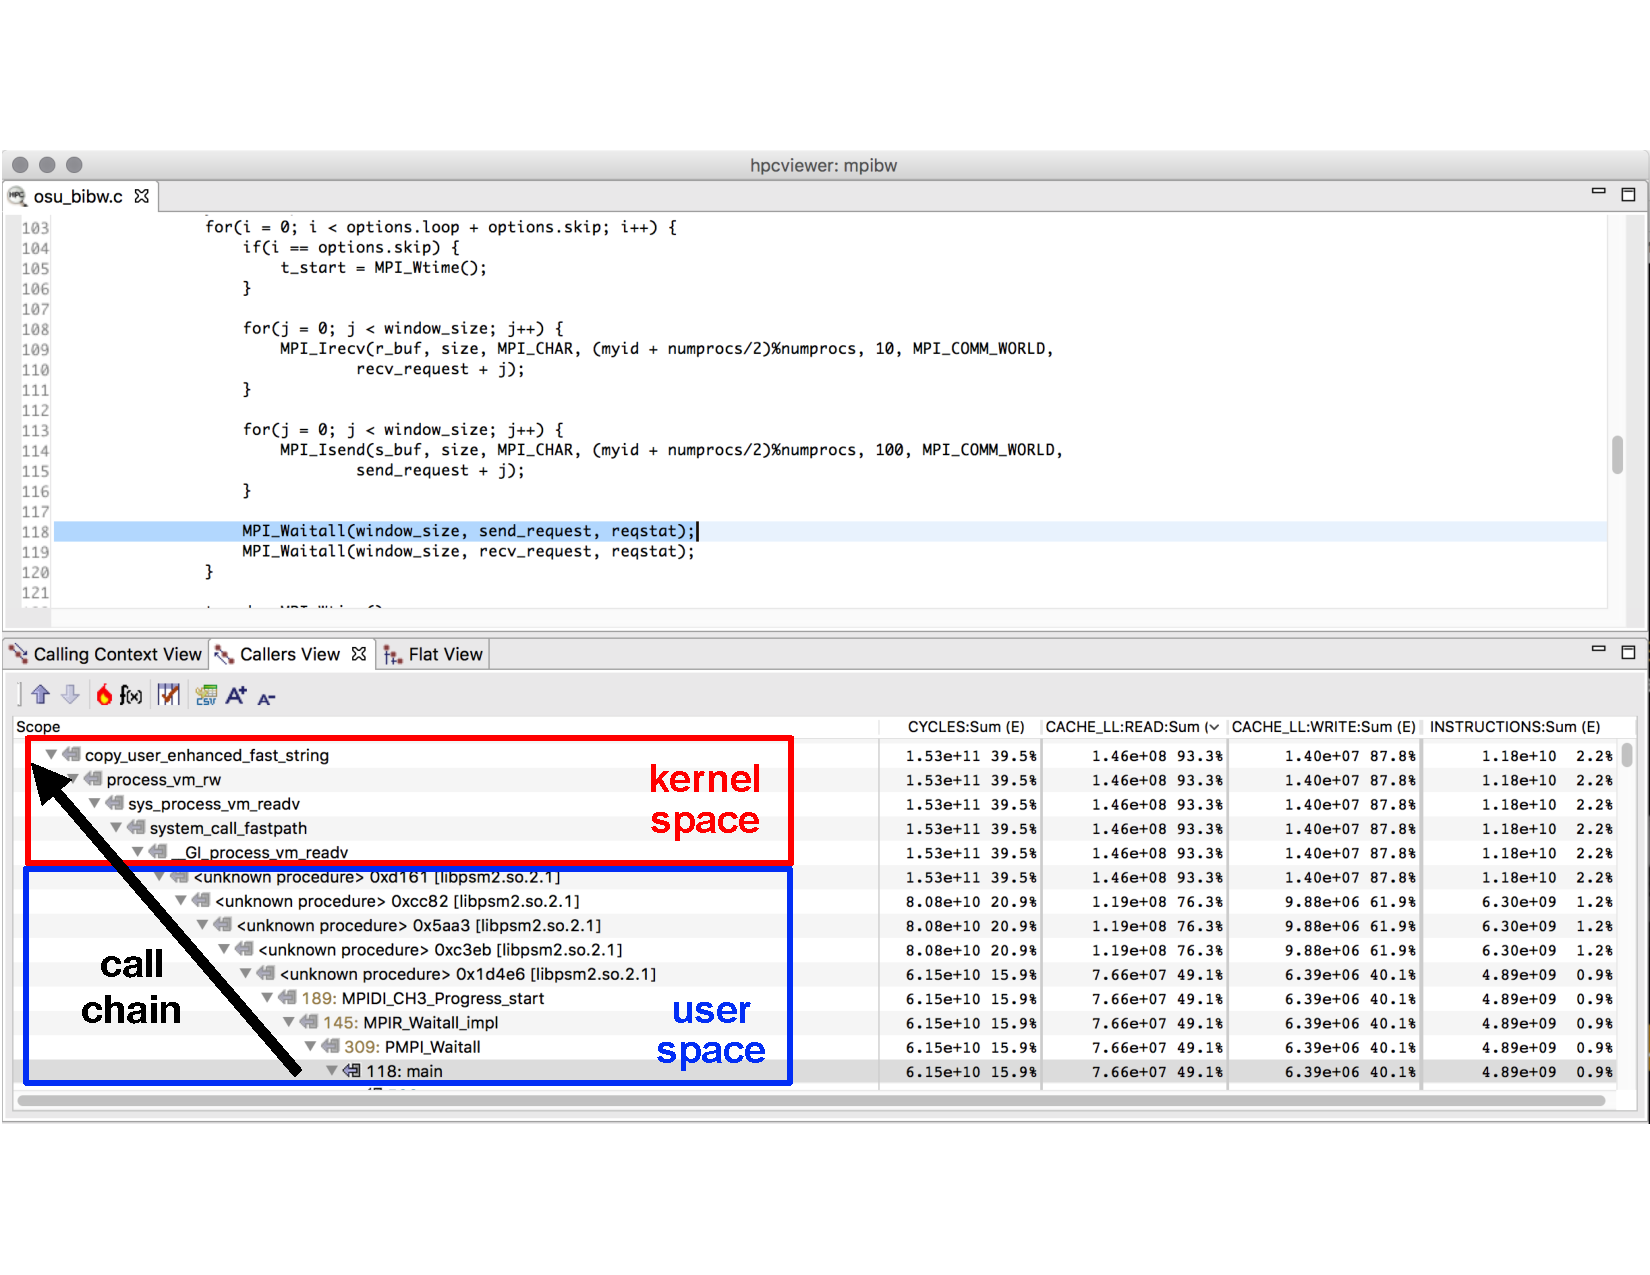
\includegraphics[width=.48\textwidth]{projects/2.3.2-Tools/2.3.2.08-HPCToolkit/hpctoolkit-kernel}
%\caption{The December 2017 release of HPCToolkit includes support for measuring and attributing performance metrics of kernel activity on behalf of an application.}
%\label{fig:hpctoolkit-kernel}
\end{subfloat}
\hfill
\begin{subfloat}[HPCToolkit GPU offloaded performance.
\label{fig:hpctoolkit-perfsuite}]%{.48\textwidth}
\centering
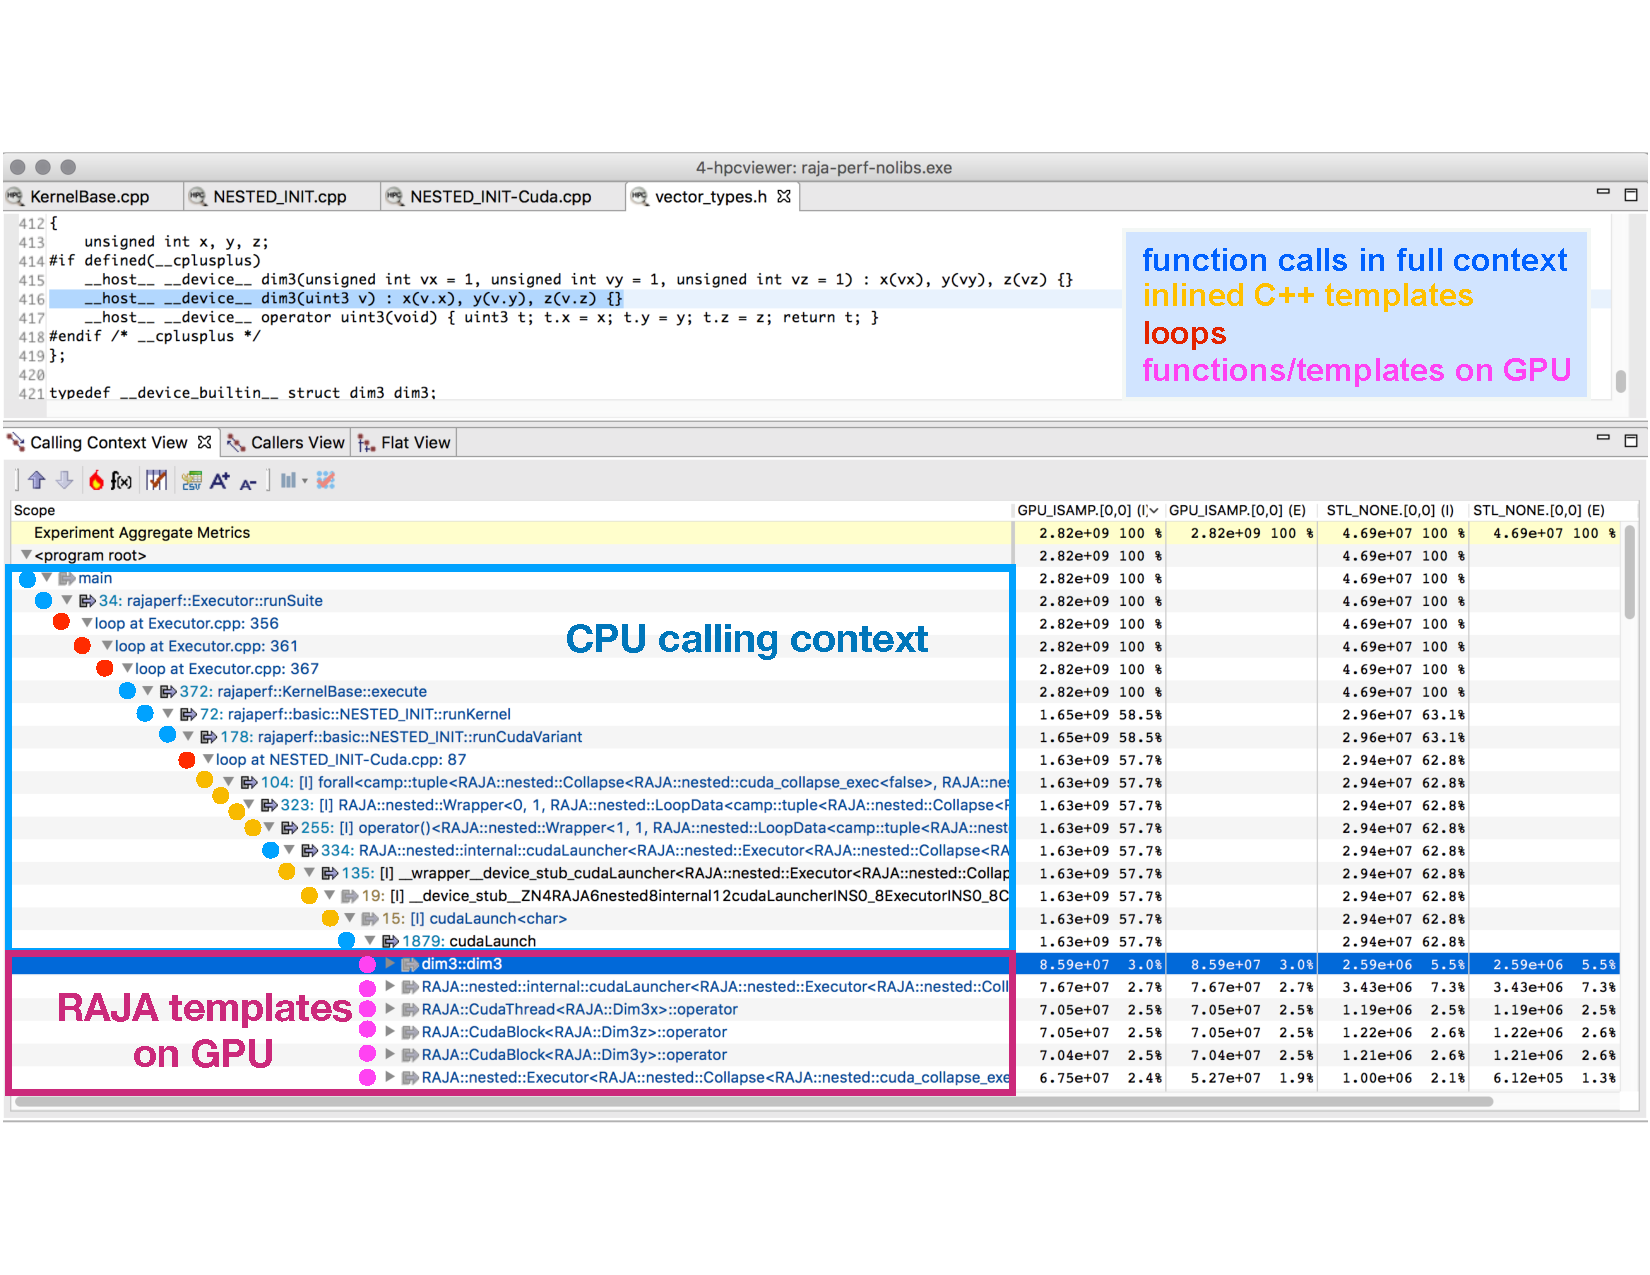
\includegraphics[width=.48\textwidth]{projects/2.3.2-Tools/2.3.2.08-HPCToolkit/hpctoolkit-perfsuite}
%\caption{HPCToolkit now measures and attributes the performance of computation offloaded to GPUs using LLNL's RAJA template-based programming model.}
%\label{fig:hpctoolkit-perfsuite}
\end{subfloat}
\caption{The December 2017 HPCToolkit release supports measuring and attributing performance metrics of kernel activity on behalf of an application.  HPCToolkit now measures and attributes the performance of computation offloaded to GPUs using LLNL's RAJA template-based programming model.}
\end{figure}
\vspace{-1ex}

\paragraph{Next Steps}

The next steps in the project are to:
\begin{itemize}
\setlength\itemsep{0em}
\item Work with the OpenMP standards committee to finalize tool interfaces as part of the emerging OpenMP standard.
\item Complete and deploy implementation of  HPCToolkit's support for measurement and analysis of code offloaded onto NVIDIA GPUs. 
%Work to integrate GPU measurement support back into the open-source {\tt libomptarget} library.
\item Integrate new support for task-based parallelism developed as part of the project's Dyninst binary analysis infrastructure into HPCToolkit's binary analyzer to accelerate analysis of large executables.
\item Complete work on data-centric performance analysis capabilities that  measure and attribute data movement costs to program variables.
\item Complete and deploy a framework for regression testing of HPCToolkit.
\item Work with DOE and Intel on performance measurement technologies for the A21 Exascale platform.
\end{itemize}

\newpage
\subsubsection{\stid{2.09} PROTEAS: Programming Toolchain for Emerging Architectures and Systems} 


\paragraph{Key  Challenges:}
Programmer productivity and performance portability are two of the most important challenges facing applications targeting future Exascale computing platforms. Application developers targeting evolving ECP architectures will find it increasingly difficult to meet these dual challenges without help from integrated capabilities that allow for flexibility, composability, and interoperability across a mixture of programming, runtime, and architectural components. In particular, an integrated programming toolchain is critical for Exascale delivery. First, it will provide a programming pathway to anticipated Exascale architectures by addressing programmability and portability concerns of emerging technology trends seen in pre-procurement machines. It will also enable ECP applications teams to explore programming options to find the most effective and productive approaches without constraining programming models or software solutions. Second, an integrated programming framework strategy will deliver solutions that will be further refined for the architecture capabilities known to be in the system procurement. This is essential for maintaining developer productivity and attaining performance portability as ECP requirements evolve.


\paragraph{Solution Strategy:}
The PROTEAS (\textit{PROgramming Toolchain for Emerging Architectures and Systems}) project is a strategic response to the continuous changes in architectures and hardware that are defining the landscape for emerging ECP systems. PROTEAS is a flexible programming framework and integrated toolchain that will provide ECP applications the opportunity to work with programming abstractions and to evaluate solutions that address the Exascale programming challenges they face. Specifically, the PROTEAS objectives are to

\begin{enumerate}
    
    \item Provide productive and performance-portable programming solutions based on directive-based methodologies that support current language paradigms and flexible prototyping of interfaces specifically directed at heterogeneous and manycore processors, deep memory hierarchies, and nonvolatile memory systems (NVM);
    
    \item Provide integrated performance assessment solutions for these programming systems that will enable automatic performance analysis and performance-driven optimization;
    
    \item Provide an integrated programming toolchain that is powerful enough to prototype the above solutions, while flexible enough to extend its functionality over time;
    
    \item Refine our toolchain and solutions through engagement with ECP applications teams who will evaluate prototypes, provide feedback, promote application readiness, and facilitate use of ECP prototype and eventual production machines; and,
    
    \item Champion our successful solutions in ECP procurements, community standards, and open-source software stacks.
    
\end{enumerate}

Our team has started with a strong existing base of relevant technological and software capabilities. Importantly, our solutions are based on our significant, continuing work with LLVM, ARES HLIR, OpenARC, and TAU. We have extensive experience and a demonstrated track record of accomplishment in all aspects of this proposed work including existing software deployments, interaction with application teams, vendor interaction, and participation in open source community and standards organizations.

Our strong emphasis on delivering an effective toolchain to application developers within the next few years emphasizes the importance of adopting an integrated programming solution that will be further refined for the architecture capabilities known to be in the Exascale system procurement. We will develop an integrated system (i.e. compilers, runtime systems, debuggers, and performance tools) suitable for deployment in the 2021 timeframe. The experience gained from this development will inform vendor collaborations, proposals to standards committees, and existing open source software to make key elements of our developed technology ready for ECP deployment, either from vendors, through the ECP SDKs, or directly from other open-source venues.

While PROTEAS will be oriented towards foreseeable architectural trends, it will not lock in to specific choices that will constrain what new hardware features it can address. Rather, it is important for the programming framework to embody interoperability, open interfaces, and flexibility in the toolchain, allowing it to pursue high-value solutions as opportunities arise and thereby achieve Exascale performance potential. 

\paragraph{Recent Progress:}

Our recent work has focused on five topics:

\begin{enumerate}
    
    \item OpenACC and Clacc~\cite{clacc:2018:denny}. Develop production-quality, standard-conforming OpenACC compiler and runtime support as an extension of clang/LLVM. See \S\ref{s:clacc}.
    
    \item Papyrus~\cite{Kim:2017:DIP,Kim:2017:PHP} for portability across NVM architectures. 
    Develop a portable interface to NVM architectures to provide massive, persistent data structures as required by many applications.
    See \S\ref{s:papyrus}.
    
    \item Performance analysis with Tau by adding additional functionality for new architectures. 
    Improve a widely-used performance analysis framework by adding functionality for new architectures and software systems.
    See \S\ref{subsubsect:tau}.

    \item Improving LLVM. In collaboration with numerous other ECP projects, PROTEAS is contributing improvements to the LLVM compiler infrastructure. These improvements include simple bugfixes to the existing infrastructure, monitoring Flang progress, developing Clacc (see \S\ref{s:clacc}), and contributing to the development of a new parallel intermediate representation (see \url{https://github.com/Parallel-IR/llvm-pir/wiki}).
    
    \item Outreach and collaboration with ECP applications teams. 
    We have interacted with over a dozen applications teams to help prepare their applications for ECP. See \S\ref{s:clacc}, \S\ref{s:papyrus}, and \S\ref{subsubsect:tau}.
    
\end{enumerate}

\paragraph{Next Steps:}

Our next efforts are:

\begin{enumerate}
	\item Clacc. Complete Clacc support for a prescriptive interpretation of OpenACC by lowering OpenACC directives to use the existing LLVM OpenMP infrastructure.
    
	\item Papyrus. Improve support for versioning and other performance improvements.
    
    \item Tau. Improve performance instrumentation for deep memory hierarchies in Tau, focusing primarily on various GPUs and emerging NVM.
    
    \item LLVM Parallel IR. Develop a conceptual prototype for mapping LLVM Clang operations to the proposed Parallel IR, and implement a prototype.

\end{enumerate}

\newpage
\subsubsection{\stid{2.09} PROTEAS | TAU Performance System}\label{subsubsect:tau}

\paragraph{Overview} 
The TAU Performance System is a versatile profiling and tracing toolkit that supports performance instrumentation, measurement, and analysis.  Figure~\ref{figure:tau} gives an example of using TAU's parallel profile analysis tool, ParaProf. It is a robust, portable, and scalable performance tool for use in parallel programs and systems over several technology generations. It is a ubiquitous performance tool suite for shared-memory and message-passing parallel applications written in C++, C, Fortran, Java, Python, UPC, and Chapel. In the PROTEAS project, TAU is being extended to support compiler-based instrumentation for the LLVM C, C++, and Fortran compilers using higher-level intermediate language representation. TAU is also targeting support for performance evaluation of directive based compilation solutions using OpenARC and it will support comprehensive performance evaluation of NVM based HPC systems.  Through these and other efforts, our objective to better support parallel runtime systems such as OpenMP, OpenACC, Kokkos, ROCm, and CUDA in TAU. 

\paragraph{Key Challenges} 
Scalable Heterogeneous Computing (SHC) platforms are gaining popularity, but it is becoming more and more complex to program these systems effectively and to evaluate their performance at scale. Performance engineering of applications must take into account multi-layered language and runtime systems, while mapping low-level actions to high-level programming abstractions.  Runtime systems such as Kokkos can shield the complexities of programming SHC systems from the programmers, but pose challenges to performance evaluation tools.  Better integration of performance technology is required.  Exposing parallelism to compilers using higher level constructs in the intermediate language provides additional opportunities for instrumentation and mapping of performance data.  It also makes possible developing new capabilities for observing multiple layers of memory hierarchy and I/O subsystems, especially for NVM-based HPC systems. 

\paragraph{Solution Strategy} Compilers and runtime systems can expose several opportunities for performance instrumentation tools such as TAU.  For instance, using the OpenACC profiling interface, TAU can tap into a wealth of information during kernel execution on accelerators as well measure data transfers between the host and devices. This can highlight when and where these data transfers occur and how long they last.  By implementing compiler-based instrumentation of LLVM compilers with TAU, it is possible to how the precise exclusive and inclusive duration of routines for programs written in C, C++, and Fortran.  Furthermore, we an take advantage of the Kokkos profiling interface to help map lower level performance data to higher level Kokkos constructs that are relevant to programmers. The instrumentation at the runtime system level can be achieved by transparently injecting the TAU Dynamic Shared Object (DSO) in the address space of the executing application. This requires no modification to the application source code or the executable. 

\begin{figure}[htb]
\centering
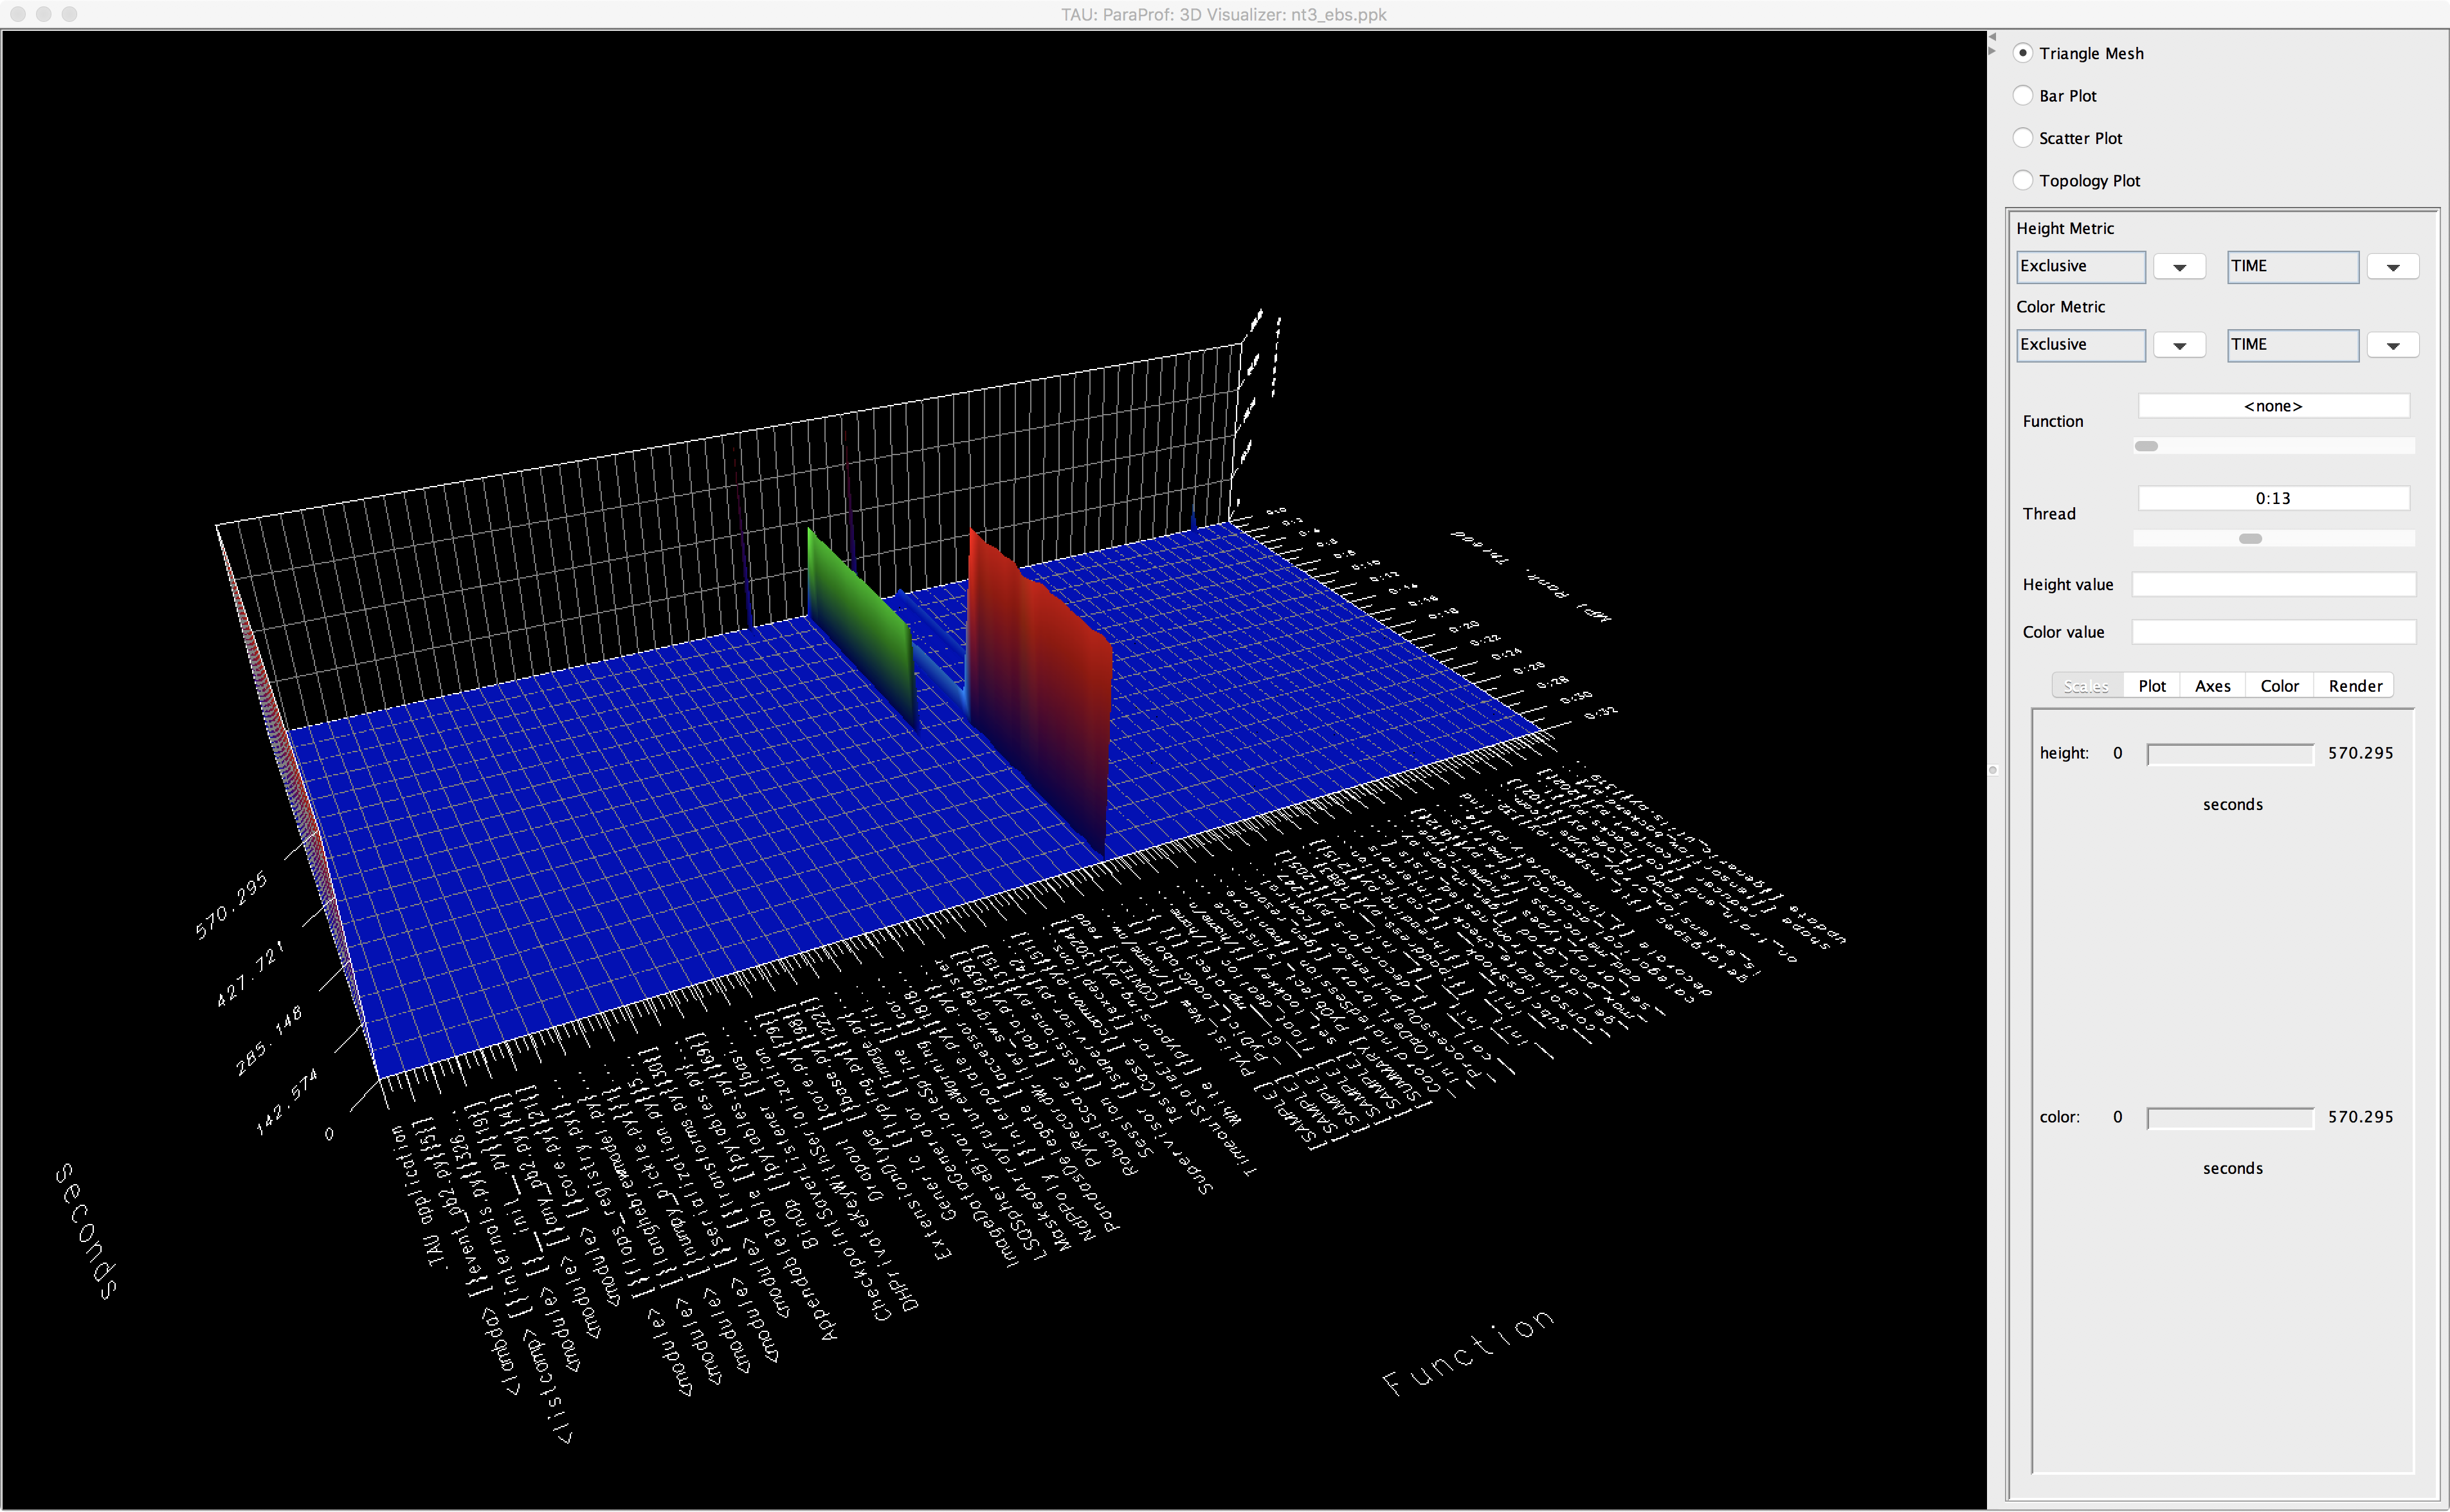
\includegraphics[width=6in]{projects/2.3.2-Tools/2.3.2.09-PROTEAS/tau-3d-candle}
\caption{
  TAU's ParaProf profile browser shows the parallel performance of the CANDLE application, where half the threads are engaged in one activity (\texttt{pthread\_cond\_wait}) while the other half is engaged in some other activity (\texttt{Eigen::internal::gebp\_kernel})..
}
\label{figure:tau}
\end{figure}

\paragraph{Recent Progress}
\begin{enumerate}
\item \textbf{CANDLE} Extended TAU to enhance performance evaluation of multii-threaded Python3 and CUDA and applied it to evaluate the performance of the CANDLE ECP Benchmarks on IBM Power and Cray XC systems. 

\item \textbf{Improved CUDA and OpenMP support} Added support for newer GPUs and enhancements to the CUPTI profiling interface in TAU, including multithreaded kernel launch support.  Further updated the OpenMP Tools Interface support in TAU, to support the evolving 5.0 standard. 

\item \textbf{NVM Measurement} Added support for LIKWID hardware counter support, which exposes NVM memory hierarchy counters to TAU.

\item \textbf{LLVM Instrumentation} Per-function selective instrumentation support for compiler-based instrumentation was impliemented in TAU, using an LLVM plugin.

\item \textbf{AMReX} TAU OpenACC measurement was demonstrated on the AMReX library.

\item \textbf{CODAR} TAU integrated measurement of ADIOS 1.13 using a callback mechanism, and runtime performance data aggregation and monitoring of a coupled fusion simulation using the Scalable Observation System (SOS).
\end{enumerate}

\paragraph{Next Steps}
\begin{enumerate}
\item \textbf{NVM instrumentation} 
Design and implement support for supporting deep memory hierarchies in TAU for supporting MCDRAM based systems. This includes support for memkind hbm-malloc and Fortran FASTMEM directives. 

\item \textbf{NVM Measurement} 
Comprehensive profiling and tracing support for NVM architectures.

\item \textbf{PHIRE} 
Improved LLVM IR-based instrumentation using PHIRE

\item \textbf{Outreach}
Continued outreach activities to demonstrate comprehensive performance evaluation support in TAU for OpenARC, LLVM, CUDA, Kokkos, ROCm, and NVM based programming frameworks for SHC platforms. 
\end{enumerate}
\newpage
\subsubsection{\stid{2.09} PROTEAS | PAPYRUS: Parallel Aggregate Persistent Storage}\label{s:papyrus}

\paragraph{Overview} 
Papyrus is a programming system that provides features for scalable, aggregate, persistent memory in an extreme-scale system for typical HPC usage scenarios. Papyrus provides a portable and scalable programming interface to access and manage parallel data structures on the distributed NVM storage. Papyrus allows the programmers to exploit large aggregate NVM space in the system without handling complex communication, synchronization, replication, and consistency models. Papyrus consists of three components, virtual file system (VFS)~\cite{Kim:2017:DIP}, C++ template container library (TCL)~\cite{Kim:2017:DIP}, and key-value store (KV)~\cite{Kim:2017:PHP}.
%Figure~\ref{fig:papyrus-fig} illustrates the overview of Papyrus.
(1) PapyrusVFS provides a uniform aggregate NVM storage image for the different types of NVM architectures. It presents an illusion of a single large NVM storage for all NVM devices available in the distributed system. Unlike other traditional kernel-level VFSs, PapyrusVFS is a lightweight user-level VFS, which is provided as a library so that applications can link to or dynamically load it. PapyrusVFS implements a subset of POSIX API related to file I/O. (2) PapyrusTCL provides a high-level container programming interface whose data elements can be distributed to multiple NVM nodes. PapyrusTCL provides three containers, including map, vector, and matrix, implemented as C++ templates. PapyrusTCL is built on top of PapyrusVFS. This enables PapyrusTCL to be decoupled from a specific NVM architecture and to present a high-level programming interface whose data elements are distributed across multiple NVM nodes transparently. (3) PapyrusKV is a novel embedded KVS implemented specifically for HPC architectures and applications to provide scalability, replication, consistency, and high performance, and so that they can be customized by the application. It stores keys and values in arbitrary byte arrays across multiple NVMs. PapyrusKV provides configurable consistency technique controlled by the application during the program execution dynamically to meet application-specific requirements and/or needs. It also supports fault tolerance and streamlined workflow by leveraging NVM's persistence property.

%\begin{figure}[htb]
%    \centering
%    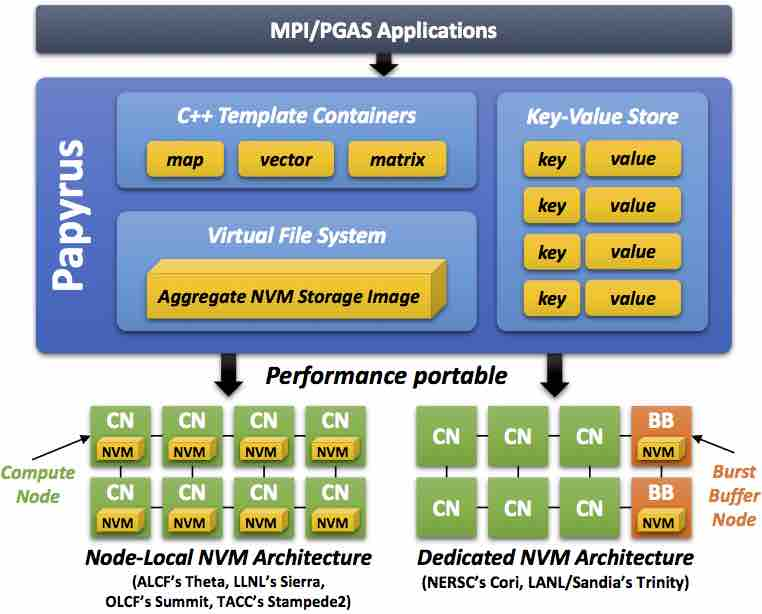
\includegraphics[width=5in]{papyrus-fig}
%    \caption{\label{fig:papyrus-fig}Papyrus consists of three components, virtual file system, C++ template containers, and key-value store}
%\end{figure}

\paragraph{Key Challenges}
In HPC, NVM is quickly becoming a necessary component of future systems, driven, in part, by the projections of very limited DRAM main memory per node and plateauing I/O bandwidth. More concretely, recently-announced DOE systems, such as NERSC's Cori, LANL/Sandia's Trinity, LLNL's Sierra, OLCF's Summit, TACC's Stampede2, and ALCF's Theta, include some form of NVM. This NVM will be used in two fundamental ways. First, it will be used as a cache for I/O to and from the traditional HDD-based external parallel file systems. In this case, most scientists believe that the caching can be implemented transparently, shielding complexity from the applications and users. Second, NVM will be used as an extended memory to provide applications with access to vast amounts of memory capacity beyond what is feasible with DRAM main memory. More interestingly, in HPC, this extended memory can be aggregated into a much larger, scalable memory space than that provided by a single node alone. In this second case, however, no portable and scalable programming systems exist.

\paragraph{Solution Strategy}
We describe our key goals for Papyrus: high performance, scalability, portability, interoperability with existing programming models, and application customizability. First, \textbf{high performance} is a clear need in HPC. The design of Papyrus should provide the opportunity to exploit NVM resources efficiently. Second, \textbf{scalability} is important in HPC as most of the applications must run on large sectors of the systems - thousands to hundreds of thousands of processors. Papyrus should not inhibit scalability; it should provide an interface that is able to scale as the application and system do. Third, \textbf{portability} is a necessary requirement because HPC applications must be able to run on multiple, diverse platforms at any given time. The upcoming DOE systems all have NVM integrated into the systems in different ways. Papyrus must provide both functional portability and performance portability across systems with different architectures. Fourth, \textbf{interoperability} is a practical requirement of HPC applications. Papyrus must be designed so that it can be incrementally introduced into an application without conflicting with existing HPC programming models and languages like MPI, UPC, OpenMP, OpenACC, C, C++, and Fortran. Furthermore, Papyrus should leverage characteristics of these other programming models when possible. Interoperability allows programmers to adopt Papyrus incrementally in legacy MPI applications avoiding major rewrites of the application. Fifth, \textbf{application customizability} is a key requirement to achieve high performance and scalability. HPC applications have many different usage scenarios, and thus Papyrus should have customizable parameters for key features that impact other important properties like performance and scalability.

\paragraph{Recent Progress}

Meraculous~\cite{Georganas:2014:PDB} is a state-of-the-art de novo assembler written in UPC. Its parallel algorithm for de Bruijn graph construction and traversal leverages the one-sided communication in UPC to facilitate the requisite random access pattern in the global de Bruijn graph. The de Bruijn graph is implemented as a distributed hash table with an overlapping substring of length {\it k}, referred to as a {\it k-mer}, as key and a two-letter code [ACGT][ACGT] as value as shown in \autoref{fig:papyrus-meraculous}. A hash function is used to define the affinities between UPC threads and hash table entries. We ported the distributed hash table written in UPC to a PapyrusKV database. The keys in the database are k-mers and the values are two-letter codes. The PapyrusKV runtime calls the same hash function in the UPC application to determine the owners of key-value pairs in the database by specifying the custom hash function when the database is created. Thus, the thread-data affinities in UPC and PapyrusKV are the same as shown in \autoref{fig:papyrus-meraculous}. PapyrusKV requires fewer lines of source code than UPC because it calls standard put and get API functions without implementing an application-specific algorithm for the distributed hash table construction and traversal. \autoref{fig:papyrus-meraculous-eval} shows the performance comparison between PapyrusKV and UPC of Meraculous on Cori. Both versions are built and run using Berkeley UPC, an MPI-interoperable UPC implementation. We measured the total execution time on 32, 64, 128, 256, and 512 UPC threads (32 UPC threads per node). UPC shows better performance than PapyrusKV due to its RDMA capability and built-in remote atomic operations during the graph traversal. The performance gap between UPC and PapyrusKV decreases as the number of UPC threads increases. On 512 UPC threads, PapyrusKV runs 1.5 times slower than UPC. This is mainly because of the asynchronous migration in PapyrusKV during the graph construction.

%\begin{figure}[htb]
%\centering
%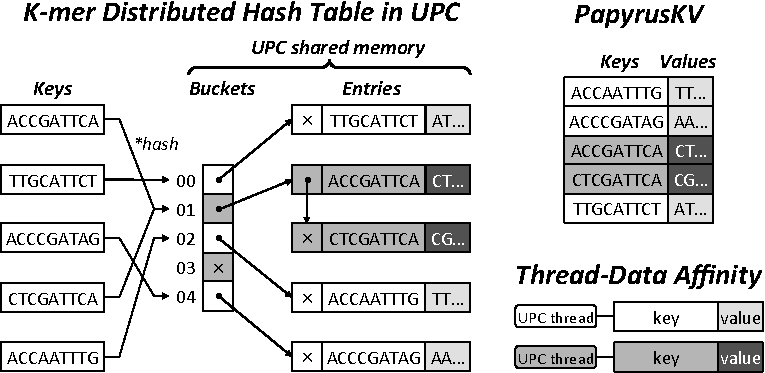
\includegraphics[width=3in]{projects/2.3.2-Tools/2.3.2.09-PROTEAS/papyrus-meraculous}
%\caption{K-mer distributed hash table implementations in UPC and PapyrusKV.}
%\label{fig:papyrus-meraculous}
%\end{figure}
%
%\begin{figure}[htb]
%\centering
%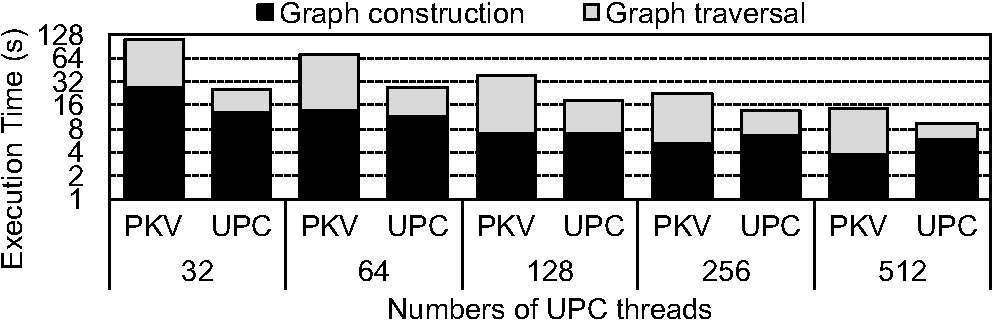
\includegraphics[width=3in]{projects/2.3.2-Tools/2.3.2.09-PROTEAS/papyrus-meraculous-eval}
%\caption{Meraculous performance comparison between PapyrusKV (PKV) and UPC on Cori.}
%\label{fig:papyrus-meraculous-eval}
%\end{figure}


\begin{figure}[t]
    \centering
    \begin{subfloat}[K-mer distributed hash table implementations in UPC and PapyrusKV.\label{fig:papyrus-meraculous}]
        \centering
        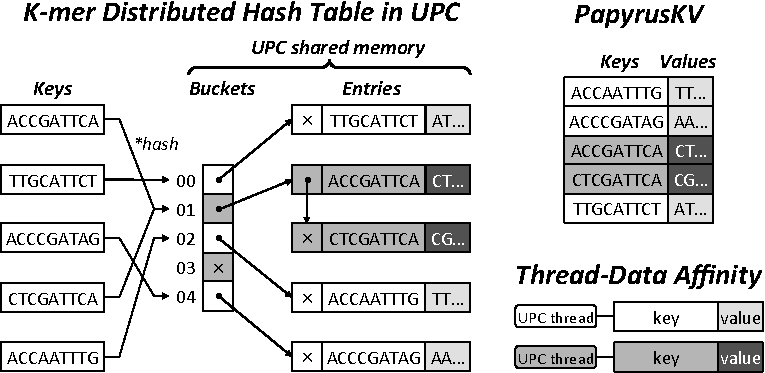
\includegraphics[width=.48\textwidth]{projects/2.3.2-Tools/2.3.2.09-PROTEAS/papyrus-meraculous}
    \end{subfloat}
    \hfill
    \begin{subfloat}[Meraculous performance comparison between PapyrusKV (PKV) and UPC on Cori.\label{fig:papyrus-meraculous-eval}]
        \centering
        \includegraphics[width=.48\textwidth]{projects/2.3.2-Tools/2.3.2.09-PROTEAS/papyrus-meraculous-eval}
    \end{subfloat}
    \caption{Using PapyrusKV for Meraculous.}
\end{figure}

%\begin{figure}[t]
%    \centering
%    \begin{subfigure}[b]{0.45\textwidth}
%        \includegraphics[width=.99\textwidth]{projects/2.3.2-Tools/2.3.2.09-PROTEAS/papyrus-meraculous}
%        \caption{K-mer distributed hash table implementations in UPC and PapyrusKV.}
%        \label{fig:papyrus-meraculous}        
%    \end{subfigure}
%    \hfill
%    \begin{subfigure}[b]{0.45\textwidth}
%        \includegraphics[width=.99\textwidth]{projects/2.3.2-Tools/2.3.2.09-PROTEAS/papyrus-meraculous-eval}
%        \caption{Meraculous performance comparison between PapyrusKV (PKV) and UPC on Cori.}
%        \label{fig:papyrus-meraculous-eval}
%    \end{subfigure}
%    \caption{Using PapyrusKV for Meraculous.}
%\end{figure}


This past year, we have added data compression and encryption to Papyrus. For data compression, the overhead of data access and movement becomes a serious bottleneck compared to compute overhead in large-scale HPC systems. We integrated data compression methods into Papyrus to achieve storage reduction and performance improvement. 
For data encryption, we need to protect sensitive data (e.g., health records, DNA data) that is being used in distributed infrastructures, and users need practical methods to secure their data throughout its lifecycle. We will introduce data encryption in Papyrus to add an extra layer of security in the complex scientific workflows.


\paragraph{Next Steps}
Our next efforts are:

\begin{enumerate}
\item \textbf{Versioning: } Versioning can be used to provide new levels of reliability and performance optimization. We will design and implement versioning in Papyrus.

\item \textbf{Performance optimization:} New APIs and hardware support is being developed for NVM technologies; we are implementing optimizations in Papyrus to take advantage of these advances.

\end{enumerate}
\newpage
\subsubsection{PROTEAS | Clacc: OpenACC in Clang and LLVM}\label{s:clacc}

\newcommand{\todo}[1]{\textbf{\textcolor{red}{#1}}}

\paragraph{Overview}

Heterogeneous and manycore processors (e.g., multicore CPUs, GPUs, Xeon Phi,
etc.) are becoming the de facto architectures for current HPC platforms and
future Exascale platforms.  These architectures are drastically diverse in
terms of functionality, performance, programmability, and scalability,
significantly increasing the complexity that ECP application developers face
as they attempt to fully utilize the available hardware.

A key enabling technology being pursued as part of the PROTEAS project is
OpenACC.  While OpenMP has historically focused on shared-memory multi-core
programming, OpenACC was launched in 2010 as a portable programming model
for heterogeneous accelerators.  Championed by institutions like NVIDIA,
PGI, and ORNL, OpenACC has evolved into one of the most portable and well
recognized programming models for accelerators today.

Despite the importance of OpenACC, the only non-academic open-source OpenACC
compiler cited by the OpenACC website is GCC \cite{openaccOrgTools}.
However, GCC has lagged behind commercial compilers, such as PGI's, in
providing production-quality support for the latest OpenACC specifications
\cite{openACCValidationSuite}.  Moreover, GCC is known within the compiler
community to be challenging to extend and, especially within the DOE, is
losing favor to clang and LLVM for new compiler research and development
efforts.

A major goal of PROTEAS is to build on clang and LLVM to develop an
open-source, production-quality OpenACC compiler ecosystem that is easily
extensible and that utilizes the latest research in compiler technology.
Such an ecosystem is critical to the successful acceleration of ECP
applications using modern HPC hardware.  We call this project \emph{clacc}.
The PROTEAS objectives for clacc are:

\begin{enumerate}

\item Develop production-quality, standard-conforming OpenACC compiler
and runtime support as an extension of clang/LLVM.

\item As part of the compiler design, leverage the clang ecosystem to enable
the future construction of source-level OpenACC tools, such as pretty
printers, analyzers, lint tools, debugger extensions, and editor extensions.

\item As the work matures, contribute OpenACC support to upstream clang/LLVM
so that it can be used by the broader HPC and parallel programming
communities.

\item Throughout development, actively contribute upstream any clang/LLVM
improvements that are mutually beneficial to both our OpenACC work and to
the broader clang/LLVM ecosystem.

% \item OpenARC is our in-house compiler for OpenACC.  We are utilizing
% OpenARC as a research platform for rapidly prototyping cutting-edge compiler
% techniques for translating and optimizing OpenACC.

\end{enumerate}

%\todo{Talk about our experience with OpenARC and how that positions us well
%to work on OpenACC?}

\paragraph{Key Challenges}

\begin{enumerate}

\item \textbf{OpenACC Support:} Developing production-quality,
standards-conforming OpenACC compiler and runtime support is a large
undertaking.  Complicating that undertaking further is the need for
optimization strategies that are competitive with existing commercial
compilers, such as PGI's, which have been developed over many years since
before the conception of the OpenACC standard.

\item \textbf{Source-to-Source:} Source-to-source translation from OpenACC
to another programming language can significantly reduce the effort to
implement OpenACC.  However, a well known issue with LLVM's compiler front
end, clang, is that its AST, the source-level representation, was designed
to be immutable.  Moreover, analysis and optimization capabilities are
implemented at the level of the LLVM intermediate representation (IR) not at
the AST level, but such capabilities would be critical for lowering
OpenACC's descriptive language to a more prescriptive language, like OpenMP.

\item \textbf{Production-Quality:} Clang and LLVM are sophisticated tools
with a complex codebase and a large team of developers who diligently screen
contributions to maintain a clean design and correct operation.  As for any
production-quality compiler, developing and contributing improvements to
clang and LLVM can be significantly more challenging and time-consuming than
for research-quality compilers.

\item \textbf{OpenMP Alternative:} We believe that OpenACC's current
momentum as the go-to directive-based language for accelerators will
continue into the foreseeable future.  Nevertheless, some potential OpenACC
adopters hesitate over concerns that OpenACC will one day be replaced by
OpenMP features.  A tool to migrate OpenACC applications to OpenMP could
alleviate such concerns, encourage adoption of OpenACC, and thus advance
utilization of acceleration hardware in ECP applications.

\end{enumerate}

\paragraph{Solution Strategy}

~
\vspace{-1em}

\begin{tabular}{@{\hspace{-1.5em}}p{.77\textwidth}p{.23\textwidth}@{}}

\begin{enumerate}

\item A key feature of the clacc design is to lower OpenACC to OpenMP.  This
design has several benefits:

\begin{enumerate}

\item By building on clang/LLVM's existing OpenMP compiler and runtime
support, it reduces the effort necessary to construct a production-quality
OpenACC implementation.

\item It facilitates repurposing for OpenACC existing OpenMP static analysis
and debugging tools.

\item It facilitates porting applications from OpenACC to OpenMP to
alleviate the aforementioned concerns about developing applications in
OpenACC.

\end{enumerate}

\item To ensure clacc's successful implementation and eventual acceptance
upstream, we have begun and will continue design discussions with the
clang/LLVM communities throughout clacc's development.

\item To handle clang's immutable AST, clacc's design reuses a clang feature
called TreeTransform, which was originally designed for C++ template
specializations.

\end{enumerate}

&

\raisebox{-\totalheight}{\includegraphics[scale=.65]{projects/2.3.2-Tools/2.3.2.09-PROTEAS/clacc.pdf}}

\end{tabular}

\vspace{-1em}

\begin{enumerate}

\setcounter{enumi}{3}

\item To take advantage of analyses and optimizations at the LLVM IR level,
we are investigating ongoing efforts to develop a parallel LLVM IR, which
clacc could use as an alternative code generation target.

\item To stage our development effort, we are initially implementing clacc
with two simplifications: we are implementing a prescriptive interpretation
of OpenACC to achieve correct behavior, and we are implementing and testing
only within C.  We will extend this implementation with the necessary
analyses and optimizations for a descriptive interpretation and for C++
afterward.  

\item Throughout clacc development, we are continuously integrating the
latest upstream clang/LLVM changes, and we are running and extending the
clang/LLVM test suites to detect regressions and incompatibilities.  We are
also investigating OpenACC benchmarks \cite{specAccel} and validation test
suites \cite{openACCValidationSuite} to ensure correct OpenACC behavior and
good performance.

% \item We will utilize OpenARC, an OpenACC compiler we have developed
% in-house as a research platform for rapidly prototyping cutting-edge
% compiler analyses and optimizations.  After a successful proof-of-concept
% implementation in OpenARC, we will port and harden such compiler techniques
% in clacc.

\end{enumerate}


\paragraph{Recent Progress}

\begin{enumerate}

\item Prototyped the translation of an initial set of OpenACC directives and
clauses to OpenMP.

\item Investigated OpenACC applications, benchmarks, and validation test
suites for use in clacc testing.  Reached out to ECP application teams who
have expressed interest in OpenACC.

\item Initiated clacc design discussions within the clang/LLVM developer
community.

\item Contributed to upstream clang/LLVM a number of fixes and other
improvements to clang attribute and printing support, the clang/LLVM testing
infrastructure, and the OpenMP implementation.

\end{enumerate}


\paragraph{Next Steps}

\begin{enumerate}

\item Complete clacc support for a prescriptive interpretation of OpenACC
for correct behavior, and continue to contribute mutually beneficial
improvements to upstream clang/LLVM as we develop them.

\item Continue clacc design discussions with the clang/LLVM developer
community.

\item Explore applications from ECP teams we have previously contacted.
	
\end{enumerate}

\newpage

\subsection{\mathlibs}
This section present projects in \mathlibs.
\newpage
\subsubsection{\stid{3.01} xSDK4ECP} 
\paragraph{Overview} The xSDK4ECP project is creating a value-added aggregation of DOE math and scientific libraries through the {\em xSDK} (Extreme-scale Scientific Software Development Kit)~\cite{xsdk:homepage}, which increases the combined usability, standardization, and interoperability of these libraries as needed by ECP. The project focuses on community development and a commitment to combined success via quality improvement policies, better build infrastructure, and the ability use diverse, independently developed xSDK libraries in combination to solve large-scale multiphysics and multiscale problems.  We are extending draft xSDK package community policies and developing interoperability layers among numerical libraries in order to improve code quality, access, usability, interoperability, and sustainability. Focus areas are (1) coordinated use of on-node resources, (2) integrated execution (control inversion and adaptive execution strategies), and (3) coordinated and sustainable documentation, testing, packaging, and deployment.

xSDK4ECP is needed for ECP because it enables ECP apps such as ExaAM and ExaWind to seamlessly leverage the entire scientific libraries ecosystem.  For example, ExaWind has extremely challenging linear solver scaling problems.  xSDK4ECP provides access to all scalable linear solvers with minimal changes.  xSDK4ECP is also an essential element of the product release process for ECP ST.  xSDK4ECP provides an aggregate build and install capability for all ECP math libraries that supports hierarchical, modular installation of ECP software.  Finally, xSDK4ECP provides a forum for collaborative math library development, helping independent teams to accelerate adoption of best practices, enabling interoperability of independently developed libraries and improving developer productivity and sustainability of the ECP ST software product.

\paragraph{Key Challenges}
The complexity of application codes is steadily increasing due to more sophisticated scientific models.  While some application areas will use Exascale platforms for higher fidelity, many are using the extra computing capability for increased coupling of scales and physics.  Without coordination, this situation  leads to difficulties when building application codes that use 8 or 10 different libraries, which in turn might require additional libraries or even different versions of the same libraries.

The xSDK represents a different approach to coordinating library development and deployment.  Prior to the xSDK, scientific software packages were cohesive with a single team effort, but not across these efforts. The xSDK goes a step further by developing community policies followed by each independent library included in the xSDK.  This policy-driven, coordinated approach enables independent development that still results in compatible and composable capabilities.

\paragraph{Solution Strategy}

The xSDK effort has two primary thrusts:
\begin{enumerate}
	\item \textbf{Increased interoperability:} xSDK packages can be built with a single Spack package target.  Furthermore, services from one package are accessible to another package.
	\item \textbf{Increased use of common best practices:}  The xSDK has a collection of community policies that set expectations for a package, from best design practices to common look-and-feel.
\end{enumerate}

xSDK interoperability efforts began first with eliminating incompatibilities that prohibited correct compilation and integration of the independently developed libraries.  These issues include being able to use a common version of a library such as SuperLU by PETSc and Trilinos.  The second, and ongoing phase is increased use of one package's capabilities from another.  For example, users who build data objects using PETSc can now access Trilinos solvers without copying to Trilinos data structures.

xSDK community package policies~\cite{xsdk-policies:homepage,
xSDK-community-package-policies2018} are a set of minimum requirements (including topics of configuring, installing, testing, MPI usage, portability, contact and version information, open source licensing, namespacing, and repository access) that a software package must satisfy in order to be considered xSDK compatible. The designation of xSDK compatibility informs potential users that a package can be easily used with others. 

xSDK community installation policies~\cite{xSDK-community-installation-policies2017} help make configuration and installation of xSDK software and other HPC packages as efficient as possible on common platforms, including standard Linux distributions and Mac OS X, as well as on target machines currently available at DOE computing facilities (ALCF, NERSC, and OLCF) and eventually on new Exascale platforms.

Community policies for the xSDK promote long-term sustainability and interoperability among packages, as a foundation for supporting complex multiphysics and multiscale ECP applications. In addition, because new xSDK packages will follow the same standard, installation software and package managers (for example, Spack~\cite{gamblin+:sc15}) can easily be extended to install many packages automatically.


\paragraph{Recent Progress}

Figure~\ref{fig:xsdk-schematic} illustrates a new {\em Multiphysics
	Application C}, built from two complementary applications that can
readily employ any libraries in the xSDK, shown in green.  Current xSDK member packages (xSDK-0.4.0, released December 2018) are the four founding libraries
(hypre~\cite{hypre:homepage}, PETSc~\cite{petsc:homepage}, SuperLU~\cite{superlu:homepage}, and Trilinos~\cite{trilinos:homepage}), three libraries added in xSDK-0.3.0, released December 2017 (MAGMA~\cite{magma:homepage}, MFEM~\cite{mfem:homepage}, and SUNDIALS~\cite{sundials:homepage}), and ten more libraries added in this release, including seven with DOE support (AMRex~\cite{amrex:homepage}, DTK~\cite{dtk:homepage}, Omega\_h~\cite{omega_h:homepage}, PLASMA~\cite{plasma:homepage}, PUMI~\cite{pumi:homepage}, STRUMPACK~\cite{strumpack:homepage}, and Tasmanian~\cite{tasmanian:homepage}) and three in the broader community (deal.II~\cite{deal.ii:homepage}, PHIST~\cite{phist:homepage}, and SLEPc~\cite{slepc:homepage}).  
Application domain components are represented
in orange.  Of particular note is Alquimia~\cite{alquimia:homepage}, a domain-specific interface
that support uniform access to multiple biogeochemistry capabilities, including
PFLOTRAN~\cite{pflotran:homepage}.  Additional libraries are working toward becoming xSDK member packages and plan to participate in future xSDK releases.
\begin{figure}[htb]
	\centering
	\includegraphics[width=6in]{projects/2.3.3-MathLibs/2.3.3.01-xSDK/xSDK-diagram.png}
	\caption{\label{fig:xsdk-schematic}The December 2018 release of the xSDK contains many of the most popular math and scientific libraries used in HPC.  The above diagram shows how multiphysics and multiscale applications can readily access xSDK packages.}
\end{figure}

% The arrows among the xSDK libraries indicate current support for
% a package to call another to provide scalable linear solvers
% functionality on its behalf.  For example, {\em Application~A} could
% use PETSc for an implicit-explicit time advance, which in turn could
% interface to SuperLU to solve the resulting linear systems with a
% sparse direct solver.  {\em Application~B} could use Trilinos to solve
% a nonlinear system, which in turn could interface to hypre to solve
% the resulting linear systems with algebraic multigrid.  Of course,
% many other combinations of solver interoperability are also possible.
Each xSDK member package uses or can be used with one or more xSDK packages, and the connecting interface is regularly tested for regressions.  
The sites \url{https://xsdk.info/example-usage} and 
\url{https://xsdk-project.github.io/ATPESC2018HandsOnLessons}, as well as
\cite{Klinvex-xSDKTrilinos} provide examples of
xSDK usage, including interoperability among linear solvers in hypre,
PETSc, SuperLU, and Trilinos.


\paragraph{Next Steps}


Our next efforts are:
\begin{enumerate}
	\item \textbf{Include more libraries:} xSDK4ECP will continue efforts to expand the number of participating packages, adapt community policies, and exploit increased interoperability.  We are coordinating with broader SDK efforts and working toward the inclusion of additional domain application packages.
	\item \textbf{Extend application usage:}  xSDK4ECP will continue partnering with application teams to evaluate the effectivness of current functionality and to motivate new capabilities.
% 		\item \textbf{Process control transfer interfaces:} The ever-increasing use of concurrency within the top-level MPI processes requires that computational resources used by an application or library can be transferred to another library. Transfer of these resources is essential for obtaining good performance.  The xSDK project will develop interfaces to support sharing and transfer of computational resources.
	
\end{enumerate}

\newpage
\subsubsection{hypre} 


\paragraph{Overview} 
The {\sl hypre} software library \cite{hypre,hypre_design_impl_2006} provides high performance preconditioners and solvers for the solution of large sparse linear systems on massively parallel computers, with particular focus on algebraic multigrid solvers. One of {\sl hypre}’s unique features is the provision of a (semi)-structured interface, in addition to a traditional linear-algebra based interface. The semi-structured interface is appropriate for applications whose grids are mostly structured, but with some unstructured features. Examples include block-structured grids, composite grids in structured adaptive mesh refinement (AMR) applications, and overset grids. These interfaces give application users a more natural means for describing their linear systems, and provide access to methods such as structured multigrid solvers, which can take advantage of the additional information beyond just the matrix. Since current architecture trends are favoring regular compute patterns to achieve high performance, the ability to express structure has become much more important. The {\sl hypre} library provides both unstructured and structured multigrid solvers, which have shown excellent scalability on a variety of high performance computers, e.g Blue Gene systems (unstructured solver BoomerAMG has scaled up to 1.25 million MPI cores with a total of 4.5 million hardware threads). It is used by many ECP application teams, including ExaAM, Subsurface, ExaWind, CEED, and more. It requires a C compiler and an MPI implementation, but it also runs in an OpenMP environment. It has some GPU capabilities.
\paragraph{Key  Challenges}

While {\sl hypre}'s solvers contain much parallelism, their main focus is the solution of sparse linear systems, leading to  very large demands on memory bandwidth. In addition, the use of multiple levels, while greatly aiding convergence of the solvers, leads to decreasing systems sizes, number of operations and parallel efficiencies on coarser levels. Particularly the unstructured algebraic multigrid solver BoomerAMG\cite{HeYa2002}, which is {\sl hypre}'s most often used preconditioner, suffers from increasing communication complexities on coarser levels. Coarse grid operators are generated by multiplying three matrices leading to increasing numbers of nonzeroes per row in the resulting matrices and with it increasing numbers of neighbor processes. While BoomerAMG's solve phase mainly consists of matrix vector products and smoothing operations, which are fairly straight forward to parallelize, even on a GPU, its setup phase is highly complex, including many branches, a lot of integer operations as well as some sequential passages. Current  interpolation strategies that lead to best convergence and performance on distributed memory machines are not suitable for implementation on GPUs or similar architectures requiring extreme parallelism. There are several algorithms that are more suitable for GPUs, such as direct interpolation, which however leads to degraded convergence. It could possibly be improved using Jacobi interpolation. All these options would need to be implemented and tested on GPUs. Since {\sl hypre} is a mature product with many solvers and interdependent features, any significant changes that affect the whole library, are tedious and require much testing to ensure that the library stays backward compatible and no features are broken.

\paragraph{Solution Strategy}

Since the upcoming computer architectures are heterogeneous with accelerators, it was very important to enable {\sl hypre} for GPUs. We looked into various options, such as the use of CUDA, OpenMP 4.5, as well as RAJA and Kokkos. We limited the latter two options to the structured interface and solvers which are more natural candidates for such an approach due to their use of macros, called BoxLoops, for loops.
Since computer architectures continue to change rapidly, it is important to come up with strategies that will facilitate future porting of the software. Therefore we decided to develop a new memory model that addresses the use of different memory locations.

\paragraph{Recent Progress}

Under internal LLNL funding we pursued the following ECP-related tasks: enabling portions of several solvers for GPUs, and introducing a new memory model that is based on an abstract machine model.

We  implemented the new memory model. The new model modified {\sl hypre}'s memory allocation and copying routines to include memory allocations: HYPRE$\_$MEMORY$\_$HOST, HYPRE$\_$MEMORY$\_$DEVICE and HYPRE$\_$MEMORY$\_$SHARED. It also includes a new routine SetExecutionMode that can be used to define where the current code can be run.
The new model can be mapped to the actual hardware in a variety of ways through the configure process, e.g., a host-only machine (all allocations are just mallocs) or with or without unified memory. Since it is based on an abstract machine model, it is expected that it will increase portability to future architectures. The implementation of the model was very intensive, since it affected the whole library. 

In addition, we implemented various GPU capabilities in {\sl hypre}. For the structured solvers, SMG and PFMG\cite{AsFa1996}, both setup and solve phase can now completely be run on GPUs, using both CUDA or OpenMP4.5, and do not require unified memory. In addition, options to use RAJA and Kokkos are available, albeit not well tested yet. Figure \ref{fig:pfmg} shows the performance of the total run times, including both setup and solve phase, for our fastest performing multigrid solver PFMG-CG for a 7-point 3D Laplace problem using 32 million grid points per node, comparing performance on the CPU only utilizing all its cores, to running the same problem on the GPUs using CUDA and OpenMP 4.5.

\begin{figure}
\centering
\includegraphics[width=5in]{projects/2.3.3-MathLibs/2.3.3.01-xSDK/PFMG-PCG.png}
\caption{\label{fig:pfmg} Performance of PFMG-PCG on Ray at LLNL, using Power 8 CPUs and Pascal GPUs}
\end{figure}

Porting the unstructured solver, BoomerAMG turned out to be far more complex. Currently only the solve phase can be run on the GPU for select smoothers, mainly Jacobi smoothers, and requires unified memory. The setup phase can currently be performed on the CPU only.


\paragraph{Next Steps}

Our most immediate plans are to improve the efficiency of interfacing applications with {\sl hypre}'s solvers. This includes removal of unnecessary copies, and increasing use of threading, wherever possible. We plan to remove the requirement to use unified memory for BoomerAMG and want to increase the portions of its solve phase that are not GPU-enabled yet, but are well suited for GPUs, e.g. polynomial smoothers. Further out we would like to investigate how to enable the setup phase for GPUs, initially porting algorithms that are suitable as well as finding ways to improve convergence where necessary.
In addition, we would like to work with ECP application teams who are using {\sl hypre} or would like to use it, to achieve best performance by tuning the solvers for them and potentially implementing suitable algorithmic changes. One example would be the implementation of ICGS-GMRES to improve ExaWind's solve times.

Other interesting topics that could impact ECP applications, but are currently pursued under SciDAC funding is the development of parallel smoothers that lead to better convergence than Jacobi, such as ILU related methods, as well as the development of multigrid solvers that are more capable to take advantage of the structure of a problem.


\newpage
\subsubsection{The Flexible Computational Science Infrastructure (FleCSI) Project} 

\paragraph{Overview} 

FleCSI\cite{FleCSI} is a compile-time configurable framework designed to
support multi-physics application development. As such, FleCSI attempts
to provide a very general set of infrastructure design patterns that can
be specialized and extended to suit the needs of a broad variety of
solver and data requirements. Current support includes multi-dimensional
mesh topology, mesh geometry, and mesh adjacency information,
n-dimensional hashed-tree data structures, graph partitioning
interfaces, and dependency closures, e.g., to identify data dependencies
between distributed-memory address spaces.

FleCSI also introduces a functional programming model with control,
execution, and data abstractions that are consistent with state-of-the-art
task-based runtimes such as Legion\cite{Bauer:2012:LEL:2388996.2389086}
and Charm++\cite{Kale:1993:CPC:165854.165874,
Kale:1993:CPC:167962.165874}.  The FleCSI abstraction layer provides the
developer with insulation from the underlying runtime, while allowing
support for multiple runtime systems, including conventional models like
asynchronous MPI\cite{TheMPIForum:1993:MMP:169627.169855}.  The intent
is to give developers a concrete set of user-friendly programming tools
that can be used now, while allowing flexibility in choosing runtime
implementations and optimizations that can be applied to architectures
and runtimes that arise in the future.

FleCSI uses static polymorphism, template meta-programming techniques,
and other modern C++ features to achieve high runtime performance,
customizability, and to enable DSL-like features in our programming
model. The FleCSI program structure adopts a three-tiered approach: a
low-level core library that is specialized by a mid-level layer to
create high-level application interfaces that hide the complexity of the
underlying templated classes. This structure facilitates separation of
concerns, both between developer roles, and between the structural
components that make up a FleCSI-based application.

As an example of how this works in practice, consider the FleCSI mesh
topology type:

The low-level mesh interface is parameterized by a policy, which defines
various properties such as mesh dimension, and concrete entity classes
corresponding to each topological domain and dimension. The mesh policy
defines a series of tuples in order to declare its entity types for each
topological dimension and domain, and select connectivities between each
entity. FleCSI supports a specialized type of localized connectivity
called a {\it binding}, which connects entities from one domain to
another domain.

FleCSI separates mesh topology from geometry, and the mesh--from the
topology's perspective--is simply a connected graph. Vertex coordinates
and other application data are part of the {\it state model}. Our
connectivity computation algorithms are based on
DOLFIN\cite{Logg:2010:DAF:1731022.1731030}.  Once vertices and cells
have been created, the remainder of the connectivity data is computed
automatically by the mesh topology through the following three
algorithms: {\it build}, {\it transpose}, and {\it intersect}, e.g.,
{\it build} is used to compute edges using cell-to-vertex connectivity
and is also responsible for creating entity objects associated with
these edges. From a connectivity involving topological dimensions
$D_1 \rightarrow D_2$, transpose creates connectivity $D_2 \rightarrow D_1$.
Intersect, given $D_1 \rightarrow D'$ and $D' \rightarrow D_2$, computes
$D_1 \rightarrow D_2$.  

The low-level mesh topology provides a set of iterable objects that a
mid-level specialization can make available to an application to allow,
at a high-level, iteration through connectivities using an intuitive
{\it ranged-based for} syntax, e.g., forall cells $c_i$, forall edges
$e_i$ of cell $c_i$. Entities can be stored in sets that also support
range-based for iterations and enable set operations such as union,
intersection, difference, and provide functional model capabilities with
{\it filter}, {\it apply}, {\it map}, {\it reduce}, etc.

\paragraph{Key Challenges}

As part of the LANL ATDM effort, FleCSI is one component in a rapidly
shifting environment of new software and simulation approaches. This
poses several challenges. In particular, the fast evolution of both the
runtime backends used by FleCSI, and the applications that are built on
top of it make development of FleCSI itself a challenge. Because FleCSI
is the fulcrum of a complicated co-design process, it is exposed to
instabilities and design challenges from above and below.

FleCSI also faces the challenge of developing a programming model that
can span the diverse set of system and node-level architectures for
planned and current DOE procurements. Although there is a consistent
theme of increased parallelism and scale, the details of individual
processor and accelerator architectures present subtly different models
of fine-grained parallelism that prove challenging to abstract.

Finally, FleCSI is also seeking to develop fundamental data structures
and abstractions that will enable a new and sustainable development
process that also satisfies the scope of the LANL ATDM project. This
requires careful investigation of requirements and interface design that
are essentially collaborative, and reach across institutional and
cultural barriers within our organization. These relationships are often
challenging to negotiate, and require maturity and a broad knowledge
base.

\paragraph{Solution Strategy}


Our general strategy is one of communication and co-design, whereby, we
work in carefully constructed, multi-disciplinary teams to identify
gaps in the FleCSI model, design and implement abstractions to fill
these gaps, and then verify them in compact applications. To address
the challenge of operating in a fluid design environment, we often
freeze several components of the application and/or backend runtime to
isolate a particular area for refactoring or enhancement. This approach
requires a modular design, which is one of the cornerstones of the
FleCSI project, and one that has been successfully exercised in several
instances.

\paragraph{Recent Progress}

Recent progress on the FleCSI project has seen the addition of several
new storage classes for representing unstructured and sparse data. In
particular, we have added \textit{sparse} and \textit{ragged} storage
classes. The sparse storage class provides an interface to logically
sparse data, e.g., that might arise in the representation of
multi-material models or sparse matrices. The ragged storage type is
similar, but does not have the notion of columnar indices. Both of these
storage types allow dynamic resizing and mutability of the sparsity
structure of the represented data. Additionally, we have added
\textit{global} and \textit{color} storage classes that allow the
representation of simulation state that is either a singleton, or that
is on a per-color (the task version of an MPI rank) basis, respectively.

Other recent enhancements include a simplified and improved
interoperability interface for managing and interacting with MPI tasks,
an improved futures interface, and C++ language extensions for
fine-grained data parallel operations.

\paragraph{Next Steps}

Future work will include the design and implementation of a
\textit{set topology} data structure that is suitable for representing
several different classes of particles, e.g., \textit{particle-in-cell
(PIC)} method, \textit{material-point method (MPM)}, and
\textit{Monte Carlo (MC)} methods. We are also working to incorporate
changes to the Legion programming model that will provide: a more formal
interface for reasoning about and managing graph coloring
\textit{dependent partitioning}, and an improved task model that will
significantly increase scalability \textit{control replication}.
Control replication is an important design improvement to Legion, as it
will allow runtime management of dynamically changing data types in a
more efficient manner than is currently possible. We will continue to
engage in co-design with runtime and application developers to refine
and improve the FleCSI model and interface.

\begin{figure}
  \centering
  \includegraphics[scale=0.6]{projects/2.3.3-MathLibs/2.3.3.02-LANL-ATDM-MathLibs/mesh.pdf}
  \caption{FleCSI unstructured mesh example from the FleCSALE application.}
  \label{fig:mesh}
\end{figure}

\newpage
\subsubsection{\stid{3.03} LLNL ATDM Math Libraries}

\paragraph{Overview}

The LLNL ATDM Mathematical Libraries project performs work in the MFEM library
\cite{MFEM} that is focused on providing high-performance mathematical algorithms
and finite element discretizations to next-gen high-order ECP/ATDM
applications. A main component of these efforts is the development of
ATDM-specific physics enhancements in the finite element algorithms in MFEM and
the MFEM-based BLAST Arbitrary Lagrangian-Eulerian (ALE) code \cite{BLAST}, in
order to provide efficient discretization components for LLNL's ATDM efforts,
including the MARBL application (ECP's LLNLApp).

A second main task in the project is the development of unique unstructured
adaptive mesh refinement (AMR) algorithms in MFEM, that focus on generality,
parallel scalability, and ease of integration in unstructured mesh
applications. The new AMR capabilities can benefit a variety of ECP apps that
use unstructured meshes, as well as many other applications in industry and the
SciDAC program.

Another aspect of the work is the preparation of the MFEM finite element library
and related codes for exascale platforms by using mathematical algorithms and
software implementations that exploit increasing on-node concurrency targeting
multiple complex architectures (e.g. GPUs). This part of the project is
synergistic with and leverages efforts from the ECP CEED co-design center.

MFEM is an open-source finite element library with ~3000 downloads/year from 70+
countries. It is freely available at \url{mfem.org}, on GitHub
at \url{github.com/mfem}, where the MFEM community includes more than 165
members), as well as via Spack and OpenHPC. The application outreach and the
integration in the ECP ecosystem is further facilitated by MFEM's participation
in ECP's xSDK project.

\paragraph{Key Challenges}

The key challenges addressed by the LLNL ATDM Mathematical Libraries project are:

\noindent
{\bf \em Robust high-order finite element methods for ALE compressible flow.}
While high-order methods offer significant advantages in terms of HPC performance,
their application to complicated ALE problems requires careful considerations to
control oscillations and ensure accuracy.

\begin{figure}[htb]
\centering
\includegraphics[width=\textwidth]{projects/2.3.3-MathLibs/2.3.3.03-LLNL-ATDM-MathLibs/mfem-amr}
\caption{\label{fig:mfem-amr}AMR implementation in MFEM allows many applications to benefit from non-conforming adaptivity, without significant changes in their codes.}
\end{figure}

\noindent
{\bf \em Scalable algorithms for unstructured adaptive mesh refinement.}
Adaptive mesh refinement is a common way to increasing application efficiency
in problems with localized features. While block-structured AMR has been
well-studied, applying AMR in unstructured settings is challenging, especially
in terms of derefinement, anisotropic refinement, parallel rebalance and
scalability.

\noindent
{\bf \em GPU porting of finite element codes.}
Due to the relatively high complexity of the finite element machinery, MFEM,
BLAST and related codes use object-oriented C++ design that allows generality
and flexibility, but poses challenges in terms of porting to GPU architectures.
Finding the right balance between generality and performance in the GPU context
is an important challenge for many finite element-based codes that remains
outstanding in the current software and programming model environment.

\paragraph{Solution Strategy}

The MFEM team has performed and documented a lot of research in
high-performance mathematical algorithms and finite element discretizations
of interest to ATDM applications
\cite{BLAST18,BLASTFCT18,BLASTFCT17,BLAST16,BLAST14,BLAST13,BLAST12,BLAST11}.
Our work has demonstrated that the high-order finite element approach can
successfully handle coupled multi-material ALE, radiation-diffusion and MHD.
We have also shown how high-order methods can be adapted for monotonicity
(positivity preservation), handling of artificial viscosity (shock capturing),
sub-zonal physics via closure models, etc.

To enable many applications to take advantage of unstructured mesh adaptivity,
the MFEM team is developing AMR algorithms at library level, targeting both
{\em conforming} local refinement on simplex meshes and {\em non-conforming}
refinement for quad/hex meshes. Our approach is fairly general, allowing for
any high-order finite element space, H1, H(curl), H(div), on any high-order
curved mesh in 2D and 3D, arbitrary order hanging nodes, anisotropic refinement,
derifenement and parallel load balancing.
An important feature of our library approach is that it is independent of
the physics, and thus easy to incorporate in apps, see Figure \ref{fig:mfem-amr}.

As part of the efforts in the ECP co-design Center for Efficient Exascale
Discretizations (CEED), the MFEM team is also developing mathematical algorithms
and software implementations for finite element methods that exploit increasingq
on-node concurrency targeting multiple complex architectures (e.g. GPUs). This
work includes the libCEED low-level API library, the Laghos miniapp, and several
other efforts available through CEED.

To reach its many customers and partners in NNSA, DOE Office of Science, academia
and industry, the MFEM team delivers regular releases on GitHub (e.g. mfem-3.3 and
mfem-3.3.2 in 2017) that include detailed documentation and many example codes.
Code quality is ensured by smoke tests with Travis CI on Linux, Mac, Windows and
nightly regression testing at LLNL.

\paragraph{Recent Progress}

Selected recent highlights:
\begin{itemize}
\item
New optimized version of parallel AMR in MFEM, including construction of parallel interpolation, parallel refinement and rebalancing, demonstrated excellent weak and strong scalability during runs on the full Vulcan BG/Q machine at LLNL (400K MPI tasks).
\item
An interface for the new TMOP mesh optimization capabilities from mfem-3.3.2 was completed in the BLAST code, so that its remesh phase can use the TMOP functionality.
\item
Completed initial version of multi-group radiation-diffusion in BLAST.
\item
Participated in the ATDM L2 milestone for MARBL, ``Demonstration of Modular Transport Capability in a Multi-Physics Code'', which included MFEM support for high-order (HO) to low-order-refined (LOR) field transfer.
\item
BLAST's closure model was improved by separating the material energies into finite element and point-based parts, avoiding L2 projections of highly oscillatory modes.
\item MFEM v3.3.2 was released with many new features including: support for high-order mesh optimization, xSDK support, integration with STRUMPACK, 5 new examples and miniapps, physical-to-reference space mapping, continuous integration testing on Linux, Mac and Windows, and more.
\item MFEM v3.3 was released with many new features including: support for PETSc, SUNDIALS, CMake, matrix-free preconditioning, parallel mesh format, 36 new integrators, 16 new examples, and more.
\item Moved main MFEM development to GitHub, including many internal branches and pull requests.
\end{itemize}

\paragraph{Next Steps}

Our next steps include:
prepare and release mfem-3.4; continue to attend and contribute to the weekly MARBL and BLAST meetings;
complete an initial draft of MFEM's unified interface extensions to support GPUs and other accelerators;
and provide support for the upcoming MARBL L2 milestones.


\newpage
\subsubsection{\stid{3.04} ATDM SNL Math Libraries} \label{subsubsect:trilinos}

\paragraph{Overview} 
The major project outcome for the SNL ATM Math Libraries project is to provide re-usable and convenient, math-related tools for component-based software engineering of Exascale apps.

This project develops and integrates scalable, modular, and cross-cutting software infrastructure components for ATDM and other future Exascale applications that utilize, where appropriate, ATDM Core CS components: Kokkos performance portability, Sacado/ROL embedded sensitivity analysis and optimization technology, DARMA asynchronous many-tasking, and DataWarehouse.  These components include:
\begin{enumerate}
\item	KokkosKernels (KK):  performance-portable sparse/dense linear algebra and graph kernels that utilize the hierarchical memory subsystem expected in future architectures;
\item	Scalable Solvers (SS):  optimal linear solver algorithms that exploit fine-grain parallelism for vector/SIMT and thread scaling and leverage next-generation execution and communication capabilities;
\item	Agile Components (AC):  tools for interface abstractions, discretization, time integration, and solution of nonlinear PDEs; and 
\item Embedded Analysis (EA):  tools for enabling advanced analysis workflows, focusing on embedded sensitivity analysis and optimization with use of derivatives for uncertainty quantification.
\end{enumerate}

This project combines algorithmic R\&D with delivery of interoperable software components that are expected to be crucial capabilities that will enable Sandia's ATDM application codes to be performance portable across next-generation computing architectures such as GPUs and Xeon Phis.  This work will include integration of these components into the application codes and improving their design and interfaces for mission relevant use cases.	


\paragraph{Key  Challenges}
There are several challenges associated with the work this project is conducting. Part of the complexity arises because profiling tools are not yet full mature for advanced architectures and in this context profiling involves the interplay of several factors which require expert judgment to improve performance.  Another challenging aspect is working on milestones that span a variety of projects and code bases. There is a strong dependence on the various application code development teams for our own team's success. In addition, we face a constant tension between the need for production ready tools and components in a realm where the state-of-the-art is still evolving.

\paragraph{Solution Strategy}
To address the challenges above, the SNL ATM Math Libraries project is taking a staged approach to profiling in regards to target architectures and the algorithms involved. We are also coordinating on a regular basis with the other projects that are involved in our work to minimize impediments. In response to the need for production ready tools, we are focusing on a hierarchical approach that involves producing robust, hardened code for core algorithms while simultaneous pursuing research ideas where appropriate.

\paragraph{Recent Progress}
In this section we provide several high-level snapshots of recent progress in the Math Libraries project
\begin{itemize}
\item The EA team has completed the integration of sensitivity analysis and ROL optimization tools with Tempus in support of transient full-space optimization.
\item The KK team completed development of a prototype for unified SIMD types as Kokkos SIMD type
\item The KK team built batched BLAS kernels based on the Kokkos SIMD type to be run on GPUs. On a P100 GPU, the Kokkoskernels triangular solve and dense matrix-matrix multiply provide up to 2x and 170x speedup, respectively, compared to NVIDIA?s cuBLAS.
\item Profiling of the miniEM application in Panzer by the SS team, using a mesh provided by EMPIRE developers, has identified memory growth in problems during setup which has led to a reduced memory footprint.
\item Initial results, gathered by the SS team, for performance of Tpetra stack (Belos,MueLu,Ifpack2) have been gathered for the solve phase on GPUs. This resulted in the identification of performance bottlenecks that either are in the process of or have been resolved.
\item The AC team completed construction and testing of the operator-split stepper in Tempus. This is required for time integrating the PIC and E-field solves.
\item The AC team implemented and verified a variable time-stepping algorithm (Denner, 2014) within Tempus for use with the BDF2 time-integration scheme and other Tempus schemes. 
\end{itemize}

\paragraph{Next Steps}
The following list details the next steps being taking by each component of the ATDM SNL Math Libraries project:

\begin{itemize}
\item The SS team is investigating, in collaboration with the University of Wyoming, the use of Multilevel solvers, which will eventually get integrated into SPARC via MueLu.
\item The KK team will continue to work on Integration of Kokkoskernels into IFPACK2 line preconditioners as well as testing on Volta GPUs.
\item The AC team will be focusing on the integration of Tempus into EMPIRE-PIC.
\item The EA team will extend the work that was done for adjoint sensitivities to transient, full-space optimization.

\end{itemize}
\newpage
\subsubsection{\stid{3.05} Enabling Time Integrators for Exascale Through SUNDIALS} 

\paragraph{Overview} 

This project is enhancing the SUNDIALS library of numerical software packages for integrating differential systems in time using state-of-the-art adaptive time step technologies for use on exascale systems.  Through software infrastructure developments, this project is enabling the efficient and robust SUNDIALS time integrator packages to easily interoperate with external linear and nonlinear solver packages developed for exascale computing.  In addition, this project is providing a many-vector capability so that SUNDIALS time integrators can more easily operate on data divided over heterogeneous architectures.  Lastly, this project is supporting the deployment and use of SUNDIALS packages within ECP applications, mainly through incorporation into the discretization-based Co-Design Centers, AMReX and CEED.

Efficient time integrators are essential for ECP because they are at the core of every time-dependent simulation application.  However, many applications do not use state-of-the-art methods, and if they do, they often do not yet use them fully on their systems.  For example, at the start of the ECP the astrophysics code, Nyx, used an adaptive integration package for solving individual reactions.  However, by applying a time integration package to a larger reaction system, the code is able to vectorize more of the calculations and get an accurate solution much faster.  By allowing for solvers tuned to exascale systems and vectors that are heterogeneous, SUNDIALS will be more applicable for use in multiphysics systems running on exascale platforms.



\paragraph{Key  Challenges}

Current implementations of efficient time integrators face challenges on many fronts.  First, integrators typically have treated the full physical problem with a single step size or have relied on low order operator splitting methods to couple physical processes at different time scales. While research is moving forward within the time integration community on methods for multirate systems, the software infrastructure needs to be in place to accommodate these schemes once they are developed.   Second, typical integrators operate on problem data in the form of vectors.  These operations suffer from low arithmetic intensity, and their efficiency is often memory bandwidth limited.  Lastly, implicit integrators, which are required in many exascale systems, require efficient linear and nonlinear solvers to be highly effective.  In addition, by applying integrator-dependent controls on these solvers, their efficiency can be significantly increased.  Applying these controls, however, often requires that information about the integrator and its progress be passed to the solver, and software must be designed to effectively pass that information while ensuring adequate encapsulation to provide ease of maintenance and software extension.

\paragraph{Solution Strategy}

This project includes a number of implementation activities that will prepare the SUNDIALS suite of time integrators for exascale systems. The main activity is a redesign of all linear solver interfaces and encapsulation of the nonlinear solvers within the time integrators in SUNDIALS.  The new linear solver interfaces will make it much easier to interface external solver packages while maintaining the efficiency of SUNDIALS integrators. Encapsulating the nonlinear solvers, will reduce redundant code and allow the time integrators to better leverage common code thus lowering the code maintenance burden with SUNDIALS.  In addition, the integrators will be able to take advantage of outside nonlinear solvers.  

This project is also introducing a set of optional fused vector kernels into SUNDIALS.  The goal of these kernels is to execute multiple vector operations at once thereby reducing the number of kernel launches in GPU environments and also reducing the number of communications required for reduction operations.  These new kernels will be added to all supplied SUNDIALS vectors and will be invoked through optional interfaces.

Lastly, this project is developing a many-vector capability for SUNDIALS.  Due to the tight data encapsulation within SUNDIALS, users are able to supply any vector they would like underneath the integrators.  This project will supply the infrastructure needed to make it easy to place a vector of vectors underneath the integrators.  This vector of vectors is essential for later implementation of time integrators that will advance various parts of the system with different time step sizes.  This many-vector capability will also ease the use of different programming environments as differing vectors can be instantiated on different parts of a hybrid machine. 

\paragraph{Recent Progress}

In September of 2017, SUNDIALS 3.0.0 including new linear solver and matrix interfaces, was released \cite{SUNDIALSweb}.  Figure \ref{fig:sunorg1} shows the new organization of SUNDIALS where separate linear solver interfaces are provided for direct and iterative linear solver methods.  These interfaces are shared across all SUNDIALS integrators.  Individual integrators have the freedom to supply specific information from the integrator that controls the linear solver.  In addition, a single interface to each external solver, such as SuperLU\_MT or KLU, is shared across the suite, as opposed to the prior situation where each integrator included its own interface to each solver.  In addition, a SUNMATRIX class was developed that can be instantiated with a dense, banded, or sparse matrix.  Again, this class is shared by all integrators.  

\begin{figure}[htb]
	\centering
	\includegraphics[width=6in]{projects/2.3.3-MathLibs/2.3.3.05-SUNDIALS/sunorg1.pdf}
	\caption{\label{fig:sunorg1}New structure of SUNDIALS showing options for the new SUNLINEARSOLVER and SUNMATRIX classes.}
\end{figure}

\paragraph{Next Steps}

During the remainder of FY18, this project team will:
\begin{enumerate}
\item Complete a release of SUNDIALS with the new fused vector routines implemented within each supplied vector and optionally used from the integrator packages.
\item Complete a release of SUNDIALS with all nonlinear solvers encapsulated and with implementations of the new nonlinear solver interfaces for both the Newton and fixed point solvers used in the integrator packages.
\end{enumerate}
ZZ
\newpage
\subsubsection{\stid{3.06} PETSc-TAO} \label{subsubsect:petsc}
\paragraph{Overview} 

Algebraic solvers (generally nonlinear solvers that use sparse linear solvers via Newton's method) and ODE/DAE 
integrators form the core computation of many numerical simulations. No scalable ``black box'' sparse solvers 
or integrators work for all applications, nor single implementations that work well for all scales of 
problem size. Hence, algebraic solver packages provide a wide variety of algorithms and implementations 
that can be customized for the application and range of problem sizes at hand. PETSc~\cite{petsc:homepage,petsc-man} 
is a widely used software library for the scalable solution of linear, nonlinear, and ODE/DAE systems and 
computation of adjoints (sometimes called sensitivities) of ODE systems. We focus on three topics: (1) partially 
matrix-free scalable solvers efficiently use many-core and GPU-based systems; (2) reduced synchronization 
algorithms that can scale to larger concurrency than solvers with synchronization points; and (3) performance 
and data structure optimizations for all the core data structures to better utilize many-core and GPU-based 
systems as well as provide scalability to the Exascale.

The availability of systems with over 100 times the processing power of today's machines compels the utilization 
of these systems not just for a single ``forward solve'' simulation (as discussed above) but rather within a 
tight loop of optimization, sensitivity analysis (SA), and uncertain quantification (UQ). This requires the 
implementation of a new, scalable library for managing a dynamic hierarchical collection of running scalable simulations, where the simulations directly feed results into the optimization, SA, and UQ solvers.  This library, 
which we call libEnsemble, directs the multiple concurrent ``function evaluations'' through the tight coupling 
and feedback described above. This work consist of two parts: (1) the development of libEnsemble and (2) the 
extension of TAO~\cite{tao-man} (our PETSc-based scalable optimization library) with new algorithms and 
software to utilize libEnsemble.

\paragraph{Key Challenges}

A key challenge for for scaling the PETSc/TAO numerical libraries to Exascale systems is that 
traditional ``sparse-matrix-based'' techniques for linear, nonlinear, and ODE solvers, as well 
as optimization algorithms, are memory-bandwidth limited.  Another difficulty is that any 
synchronizations required across all compute units--for example, an inner product or a 
norm--can dramatically affect the scaling of the solvers.

Running an ensemble of simulation requires a coordination layer that handles load balancing and
allows the collection of running simulations to grow and shrink based on feedback. Thus, this 
library must be able to dynamically start simulations with different parameters, resume 
simulations to obtain more accurate results, prune running simulations that the solvers 
determine can no longer provide useful information, monitor the progress of the simulations, 
and stop failed or hung simulations, and collect data from the individual simulations both 
while they are running and at the end.

\paragraph{Solution Strategy}

To address the scalability of the numerical libraries, we are developing new solvers and data 
structures including pipeline Krylov methods that delay the use of the results of inner products 
and norms, allowing overlapping of the reductions and other computation; partially matrix-free 
solvers using high-order methods that have high floating-point-to-memory-access ratios and
good potential to use many-core and GPU-based systems; and in-node optimizations of sparse 
matrix-matrix products needed by algebraic multigrid to better utilize many-core systems
using a thread neutral ``bypass MPI'' approach, which implements default interprocessor 
communication using MPI but bypasses the use of MPI in performance-critical regions 
for higher performance and thereby maintains MPI portability.

Our strategy for coordinating ensemble computations has been to develop libEnsemble
to satisfy our needs.  This library should not be confused with workflow-based 
scripting systems; rather it is a library that, through the tight coupling and 
feedback described above, directs the multiple concurrent ``function evaluations''
needed by optimization, SA, and UQ solvers.

\paragraph{Recent Progress}

In the past year, we have released PETSc 3.10 (available at \url{http://www.mcs.anl.gov/petsc})
that features enhanced GPU support.  In particular, PETSc’s algebraic multigrid (AMG) consists 
of two main components: the setup (coarsening) phase which has both GPU and CPU intensive 
portions and the solve stage which can run largely or completely on the GPU. A key 
requirement is minimizing the amount of communication needed between the CPU 
and GPU during both phases of the computation.  In the PETSc~3.10 release, we 
completed porting key AMG kernels for both phases to GPUs via CUDA, enabling
this code to run on a combination of the CPU and GPU.

\begin{figure}
\centering
\includegraphics[width=0.3\textwidth]{projects/2.3.3-MathLibs/2.3.3.06-PETSc-TAO/lib_ensemble}
\caption{The libEnsemble control flow showing a manager coordinating workers executing 
calculations of either simulation functions or generation functions.}
\label{fig:petsc-tao-fig}
\end{figure}

We have also developed the libEnsemble API, implemented it in Python, released 
version 0.4 (available at \url{https://github.com/Libensemble/libensemble}),
and provided a Spack installation.

\paragraph{Next Steps}

Our next efforts are:
\begin{enumerate}
  \item \textbf{Release libEnsemble with active management capabilities}: Add active management 
    capabilities into libEnsemble to set precision of the simulation and to store information 
    from simulations to evaluate objectives as they evolve. Work with application teams to 
    determine requirements on libEnsemble and provide assistance in its usage.
  \item \textbf{Release PETSc/TAO with optimized support for LCF machines and ECP applications}:
    Work with application teams to provide assistance in PETSc/Tao usage. Provide optimizations 
    based on application profiling.
\end{enumerate}


\newpage
\newcommand{\ignore}[1]{}
\subsubsection{\stid{3.07} Factorization Based Sparse Solvers and Preconditioners for Exascale} \label{subsubsect:strumpack}

\paragraph{Overview} 
% \textit{Provide an overview of your project.  You might find that the introductory text from your Fall 2017 Project Summary \url{https://confluence.exascaleproject.org/display/1ST/Fall+2017+ECP+ST+Project+Summaries} useful as a starting draft.}
In this project we will deliver factorization based sparse solvers
encompassing the two widely used algorithm variants: supernodal
(SuperLU library) and multifrontal (STRUMPACK library). STRUMPACK is
further enhanced with scalable preconditioning functionality using
hierarchical matrix algebra. Both libraries are purely algebraic,
applicable to a large variety of application domains. We will address
several challenges that arise in Exascale computing, with the following
focus areas: 
(1) Develop novel approximation algorithms that have lower
arithmetic and communication complexity with respect to the size of the
input matrix;
(2) Develop new parallelization strategies that reduce
inter-process communication and expose task parallelism and vectorization
for irregular computations involving sparse data structures to better
use on-node resources;
(3) Integrate our software into the higher level
algebraic solvers such as hypre, PETSc, Trilinos, and collaborate with
ECP application teams for application-specific and hardware-specific tuning
of the parameters space to achieve optimal efficiency of our solvers.

Our solver technology is essential for ECP, because many DOE simulation
and data analysis codes expected to run on the Exascale machines need
solutions of sparse algebraic systems, and many high fidelity simulations
involve large-scale multiphysics and multiscale modeling problems that
generate highly ill-conditioned and indefinite algebraic equations,
for which pure iterative methods such as Krylov and multigrid, albeit
readily parallelizable on large machines, cannot converge to the solution.
The factorization based algorithms being developed herein
represent an important class of methods that are indispensable building
blocks for solving those numerically challenging problems. Our software
can often be used as a reliable standalone solver, or as a preconditioner
for Krylov iterative methods, or as a coarse grid solver in multigrid
methods, just to name a few.

\paragraph{Key Challenges}
%\textit{Describe what is hard to do, why it is challenging.}
At Exascale we need to address several major challenges:
decreasing amount of memory per core, larger impact of communication
cost and load imbalance, more heterogeneous architecture.
Our new design of algorithms and codes need to focus on
reducing communication and synchronization and task scheduling 
instead of floating point operation throughput. In sparse factorization
methods, we expect new bottlenecks in parts of the code
that previously received little attention. For example, the preprocessing
step involves numerical pivoting for selecting stable pivots and
symbolic factorization, which do not yet parallelize well on manycore
architectures with fine-grained parallelism.
At Exascale, direct solvers are more likely to
be used in a preconditioning strategy, for example, in block Jacobi
preconditioning, in domain decomposition methods or as coarse-grid
solvers in algebraic multigrid, which requires repeated triangular
solves. The challenge here is to mitigate the low arithmetic intensity
and high degree of data dependency.

Compared to iterative methods, the primary bottleneck of direct solvers
is the asymptotically higher growth in memory need and floating point
operations, especially for problems from three-dimensional geometry.
It is imperative to develop novel factorization methods which require
much less memory footprint and data movement.


\paragraph{Solution Strategy}
%\textit{Describe your basic strategy for addressing the challenges.}
We will address these challenges in several thrust areas.
The new techniques will be implemented in the two software packages SuperLU
and STRUMPACK. The former is a widely used sparse direct solver based on
supernodal factorization and the latter is a newer direct
solver/preconditioner package based on multifrontal factorization 
and hierarchical low-rank matrix structures.
% Parallel pre-pivoting for both packages.

The improvements for SuperLU will be mainly in two areas: (1) develop
a communication-avoiding 3D factorization code that have provably 
lower communication complexity; (2) develop a synchronization-avoiding
triangular solve code to enable more overlap of communications of different
processes at different substitution steps.

In addition to exploiting structural sparsity as SuperLU does, STRUMPACK
also exploits data sparseness in the dense blocks of sparse factors using
low-rank representations, which leads to linear scaling $O(n)$ or $O(n \log n)$
memory and arithmetic complexity for PDEs with smooth kernels.
The developments for STRUMPACK will focus on several areas:
(1) develop robust stopping criteria --- both absolute and relative --- for
    adaptive (incremental) randomized sampling scheme to reveal numerical
    ranks in the low-rank compression routine. The goal is to use
    enough samples for stability, but not too many for efficiency;
(2) add OpenMP support for both HSS compression and ULV factorization routines,
    especially use OpenMP task construct to support irregular parallelism.
(3) reduce MPI communication in all stages of the code, including HSS
    construction, ULV factorization and triangular solve;
(4) in addition to HSS, develop codes to support other simpler low-rank
    format, such as HOLDR. The HSS format has asymptotically lower complexity
    than HOLDR, but has larger prefactor constant. We expect HSS to be more
    useful for large-scale problems while HOLDR is more useful for mid-range
    problems;
(5) work with the ECP application teams to examine their specific problem
    characteristics and develop the best clustering/ordering methods to 
    reveal low-rank structures.

\paragraph{Recent Progress}
%\textit{Describe what you have done recently.  It would be good to have some kind of figure or diagram in this section.}
In the past six months, we have made good progress in several areas.
For the latest releases of both packages, we integrated a parallel
pre-ordering algorithm called Approximate-Weight Perfect Matching (AWPM)
for pivot selection~\cite{AWPM2018}. The other improvements are:
\begin{enumerate}
\item We released a new version v6.1.0 of SuperLU\_DIST, which contains
      the following features:
      1) Improvement on strong scaling of the 
      triangular solve -- up to 4.4x faster than Version 5.x on 4000+
      cores~\cite{LiuTriSolve2018};
      2) On-node threading optimization leading up to 3x speedup on a Cori-KNL node;
\item We released a new version v3.1.0 of STRUMPACK, which contains the
      following new features:
      1) Changes to the build system for xSDK compliance;
      2) Improvements on the scalability of the HSS algorithms --
      dense matrix HSS compression is up to 4.7x faster on 8 nodes (256 cores)
      of Cori-Haswell and 2.4x faster on Cori-NKL, the HSS-embedded sparse
      factorization is up to 2.2x faster on 8 Cori-KNL nodes;
      3) Improvement in HSS ULV solve with reduced communication and more
      OpenMP support, leading up to 7x faster in matrix redistribution and
      1.4x faster in the entire solve.
\item For both STRUMPACK and SuperLU, we performed initial bottleneck study
  for two ECP applications: CEED (MFEM indefinite Maxwell simulation) and
  ExaSGD (Optimizing stochastic grid dynamics). We identified performance
  bottlenecks of the solvers, proposed remedies, and documented the
  findings in the milestone memo: 
{\url{https://jira.exascaleproject.org/secure/attachment/15207/MS-ECP-App-Bottlenecks-study-Oct-2018.pdf}}.
  The plots below show strong scaling of STRUMPACK up to 8192 cores of 
  Cori-Haswell. Numerical factorization scales well, but ParMETIS ordering 
  becomes a serious bottleneck; it is even slower than serial METIS when using
  1000+ cores. But for large problems, serial METIS cannot be run on one node.
  The symbolic analysis phase also needs improvement at large scale.
\end{enumerate}

\vspace{-.3in}
\begin{figure}[htb]
\begin{minipage}[b]{0.48\columnwidth}
\centering
\includegraphics[scale=0.7]{projects/2.3.3-MathLibs/2.3.3.07-STRUMPACK-SuperLU/periodic-cube-scaling-strumpack.pdf}
\caption{STRUMPACK scaling with ParMETIS.}
\label{fig:strumpack-parmetis-scaling}
\end{minipage}
\begin{minipage}[b]{0.48\columnwidth}
\centering
\includegraphics[scale=0.7]{projects/2.3.3-MathLibs/2.3.3.07-STRUMPACK-SuperLU/periodic-cube-scaling-strumpack_metis.pdf}
\caption{STRUMPACK scaling with METIS.}
\label{fig:strumpack-metis-scaling}
\end{minipage}
\end{figure}

\ignore{  %%%% from last period ....
\begin{enumerate}
\item We developed and evaluated a fully algebraic sparse preconditioner in 
      STRUMPACK. On top of the baseline multifrontal direct solver, we use
      low-rank compression in dense frontal matrices to obtain approximate
      factorization. We showed that our MF+HSS preconditioner is more robust
      for numerically hard problems than many alternatives. Our code
      strong scales to over 6000 cores~\cite{ghysels2017-ipdps}
      (Fig.~\ref{fig:strumpack-scaling}).
\item We developed several strategies to enhance scalability of triangular
      solve in SuperLU\_DIST. One is an asynchronous tree-based 
      broadcast/reduction scheme which reduces latency and improves
      communication load balance. Another is efficient threading implementation
      and BLAS operations. The new code is 4.4x and 6.1x faster on 4096 cores
      with one and 50 right-hand sides, respectively~\cite{LiuTriSolve2018}
      (Fig.~\ref{fig:superlu-trisolve}).
\item We developed a new communication-avoiding 3D sparse LU factorization
      (IPDPS) algorithm that has provably asymptotic lower communication
      complexity in both latency and volume. The prototype implementation
      in SuperLU\_DIST achieves up to 27x improvement over the baseline 
      2D algorithm when run on 24,000 cores of Edison at
      NERSC~\cite{sao2018}.
\item In collaboration with ExaGraph ECP project, we evaluated the performance
      of a parallel pre-ordering algorithm called Approximate-Weight Perfect
      Matching (AWPM) for pivot selection in SuperLU\_DIST. 
      For most practical problems (e.g.,DOE apps, and SuiteSparse) the 
      weights of the perfect matchings generated by AWPM often within 99\%
      of the optimum. The MPI+OpenMP implementation on Cori at NERSC scales          up to 256 nodes –-- 2500x faster than serial MC64, and up to 114x
      speedup on 256 nodes (17,408 cores) Cori-KNL~\cite{AWPM2018}.
      The interface to AWPM are already implemented in both STRUMPACK and
      SuperLU and are released.
\end{enumerate}
} %%%% ignored from last period ....


\paragraph{Next Steps} Our future efforts will focus on the following areas:
%\textit{Describe what you are working on next.}
\begin{itemize}
\item We will build detailed performance models and performance specific
  code optimizations for the ECP applications that use our solvers.
\item We will design and implement new algorithms for the GPU systems.
\end{itemize}

\ignore{  %%%% from last period ....
\begin{itemize}
\item For STRUMPACK, we will improve the performance of the HSS solve
      routine, add OpenMP and reduce communication. We will implement
      the HOLDR low-rank format.
\item For both STRUMPACK and SuperLU, we will build detailed performance
      models and performance specific code optimizations for the ECP
      applications that use our solvers.
\end{itemize}
} %%%% ignored from last period ....

%%%% FFTX sub-project
\subsubsection{\stid{3.07} Sub-project: FFTX} \label{subsubsect:fftx}

\newpage
\subsubsection{\stid{3.08} ForTrilinos}

\paragraph{Overview}

The Exascale Computing Project (ECP) requires the successful transformation and porting of many Fortran application codes in preparation for ECP platforms. A significant number of these codes rely upon the scalable solution of linear and nonlinear equations. The Trilinos Project contains a large and growing collection of solver capabilities that can utilize next-generation platforms, in particular scalable multicore, manycore, accelerator and heterogeneous systems. Trilinos is primarily written in C++, including its user interfaces. While C++ is advantageous for gaining access to the latest programming environments, it limits Trilinos usage via Fortran. Several ad hoc translation interfaces exist to enable Fortran usage of Trilinos, but none of these interfaces is general-purpose or written for reusable and sustainable external use.

ForTrilinos provides a seamless pathway for large and complex Fortran-based codes to access Trilinos without C/C++ interface code. This access includes Fortran versions of Kokkos abstractions for code execution and data management. The project uses an interface generator, SWIG, which the project is extending, to create the object-oriented Fotran wrapper code that users can access directly. This language translation will occur in both directions; ForTrilinos will provide an inversion of control functionality that enables custom extensions of the Trilinos solvers that are Fortran-based. Once the ForTrilinos project is complete, a functional, extensible suite of capabilities to access Trilinos on next-generation computing systems will be provided. Several examples of this technology will be demonstrated within ECP codes with the aim of meeting their simulation goals and illustrate the technology to other Fortran-based ECP codes. As a second benefit to ECP from this effort, the Fortrilinos approach of using SWIG to generate interfaces could be extended to other C/C++ based tools and software within the ECP stable.

\paragraph{Key  Challenges}

Developing the interfaces to the C++ libraries that provide access to cutting-edge research, such as Trilinos,  is of significant benefit to Fortran community. However, such interfaces must be well documented, sustainable and extensible, which would require significant amount of resources and investment. This is further complicated by the requirements to support heterogeneous platforms (e.g., GPUs) and inversion-of-control functionality. The manual approach to such interfaces has been shown to be unsustainable as it requires interface developers to have in-depth expertise in  multiple languages and the peculiarities in their interaction on top of the time commitment to update the interfaces with changes in the library.

ForTrilinos addresses both the issue of reducing interface generation cost through investment in tool configuration and usage to make the process as automatic as possible, and the issue of providing the full-featured interface to Trilinos library, including access to manycore, accelerator and heterogeneous solver capabilities in Trilinos.

\paragraph{Solution Strategy}

The ForTrilinos project has two primary thrusts:
\begin{enumerate}
  \item \textbf{SWIG development to support Fortran wrapping:} The new Fortran
    module for SWIG allows for automatic generation of interfaces.
  \item \textbf{Incremental wrapping of selected Trilinos functionality:}
    ForTrilinos provides robust interfaces to selected Trilinos capabilities,
    including distributed data objects, linear and nonlinear solvers.
\end{enumerate}

ForTrilinos started with developing a Fortran module for the Simplified Wrapper Interface Generator (SWIG) utility~\cite{beazley1996swig}. SWIG is used to parse C++ code and generate wrapper code, and was already used for this purpose for several dozen target languages, most notably Python. The project took the approach of adding a Fortran 2003 wrapper generator for SWIG in order to fulfill many of the critical feature requirements for ForTrilinos.

The developed SWIG/Fortran functionality allowed to proceed with automatic generation of Fortran interfaces to selected Trilinos libraries. The work is conducted in phases, with each phase increasing the number of wrapped of Trilinos packages.

The first phase, completed in the first year, developed interfaces for a critical set of features required for solving linear and eigen-problems. The second phase addresses nonlinear solver, including developing automatic approach for inversion-of-control capability. Finally, in the third phase, the challenge of interoperable heterogeneous data passing between Fortran and C++, including GPU data, is addressed, including performance testing.

\paragraph{Recent Progress}

Figure~\ref{fig:fortran_ioc} illustrates a new Inversion-of-Control~(IoC)
implementation in ForTrilinos. The new approach allows Fortran users to define
an operator by using a derived type on the Fortran side, and use Trilinos
algorithms, e.g. Krylov solvers, to solve the linear system with that operator.

\begin{figure}[htb]
    \centering
    \includegraphics[scale=0.8,width=6in]{projects/2.3.3-MathLibs/2.3.3.08-ForTrilinos/ForTrilinos_ioc}
    \caption{\label{fig:fortran_ioc}The proposed Inversion-of-Control approach
    allowing Fortran applications to define operators on Fortran side while
    still using ForTrilinos types.}
\end{figure}

This approach allows the user callback functions to interact with native Fortran
types and ForTrilinos class wrapper types. In the same vein, users would not
have to manually pass \texttt{type(C\_PTR)} instances into and out of the
callback function, as the C++ Fortran conversions can be tedious and
error-prone, which indeed is the motivation for using SWIG to generate
ForTrilinos.  Another important feature is that it allows the application code
to extend Trilinos without having to generate any new interface code, either by
hand or using SWIG. In other words, the Fortran end user should not have to know
C++ or SWIG.

\paragraph{Next Steps}

Our next efforts include:
\begin{enumerate}
  \item \textbf{Provide wrappers for more libraries:} ForTrilinos will continue
    efforts to increase the number of wrapped Trilinos libraries. The scheduled
    release of the next phase of the project will include libraries
    corresponding to nonlinear solvers, such as NOX.
  \item \textbf{Integrate developed capabilities into applications:} E3SM-MMF
    is an Earth system model development and simulation project. It relies on
    Trilinos for its implicit capabilities. The ForTrilinos project will
    integrate the developed nonlinear solver with IoC into E3SM-MMF to provide
    path forward to heterogeneous stack.
  \item \textbf{Provide interfaces for heterogeneous platforms:} ForTrilinos
    will develop support for heterogeneous memory through providing access to
    Kokkos-based interfaces in Trilinos. This will allow full exposure to
    Trilinos capabilities targeting Exascale machines.
\end{enumerate}

\newpage
\subsubsection{\stid{3.09} SLATE}\label{subsubsect:slate}


\paragraph{Overview}

The objective of the Software for Linear Algebra Targeting Exascale 
(SLATE) project is to provide fundamental dense linear algebra capabilities
to the US Department of Energy (DOE) and to the high-performance 
computing (HPC) community at large.
To this end, SLATE will provide basic dense matrix operations (e.g., matrix multiplication,
rank-k update, triangular solve),
linear systems solvers, least square solvers, singular value
and eigenvalue solvers.

The ultimate objective of SLATE is to replace the
venerable Scalable Linear Algebra PACKage (ScaLAPACK) library, 
which has become the industry standard
for dense linear algebra operations in distributed memory environments.
However, after two decades of operation, ScaLAPACK is past the end of its lifecycle
and overdue for a replacement, as it can hardly be retrofitted
to support hardware accelerators, which are an integral part of today's HPC
hardware infrastructure.

Primarily, SLATE aims to extract the full performance potential and maximum 
scalability from modern, many-node HPC machines with large numbers of cores
and multiple hardware accelerators per node.
For typical dense linear algebra workloads, this means getting close to 90\% 
of the theoretical peak performance and scaling to the full size of the machine
(i.e., thousands to tens of thousands of nodes).
This is to be accomplished in a portable manner by relying on standards like 
MPI and OpenMP.

SLATE functionalities will first be delivered to the ECP applications
that most urgently require SLATE capabilities 
(e.g., EXAALT, NWChem, QMPACK, GAMESS, and CANDLE)
and to other software libraries 
that rely on underlying dense linear algebra services (e.g., FBSS).
SLATE will also fill the void left by ScaLAPACK's inability to utilize
hardware accelerators, and it will ease the difficulties associated with ScaLAPACK's
legacy matrix layout and Fortran API.
Figure~\ref{fig:slate-architecture} shows SLATE within 
the ECP software stack.

\begin{figure}[htb]
    \centering
    \includegraphics[width=0.6\textwidth]{projects/2.3.3-MathLibs/2.3.3.09-SLATE/SLATE-architecture.jpg}
    \caption{\label{fig:slate-architecture}
    SLATE in the ECP software stack.}
\end{figure}

\paragraph{Key  Challenges}

\begin{enumerate}
\item
\textbf{Designing from the ground up:}
The SLATE project's primary challenge stems from the need to design the package
from the ground up, as no existing software package offered
a viable path forward for efficient support of hardware accelerators in
a distributed-memory environment.
\item
\textbf{Aiming at a hard hardware target:}
SLATE's acceleration capabilities are being developed in an unforgiving
hardware environment, where the computing power of the GPUs exceeds the computing
power of the CPUs, as well as the communication capabilities of the network,
by orders of magnitude.
\item
\textbf{Using cutting-edge software technologies:}
Finally, SLATE is being designed using cutting-edge software technologies,
including modern features of the C++
language, as well as fairly recent extensions of the OpenMP standard
and the MPI standard.
\end{enumerate}

\paragraph{Solution Strategy}

\begin{enumerate}
\item
\textbf{Deliberate design phase:}
The need for building SLATE from scratch was a 
primary focus of SLATE's architecture and design in the initial project
milestones. First, we conducted a careful analysis of all the relevant 
technologies---existing and emerging~\cite{abdelfattah2017roadmap}.
% \footnote{\url{http://www.icl.utk.edu/publications/swan-001}}
Then we designed the initial architecture~\cite{kurzak2017designing}.
%\footnote{\url{http://www.icl.utk.edu/publications/swan-003}}
Going forward, the development process is based on alternating
feature development with refactoring and redesign
of the underlying infrastructure.
\item
\textbf{Accelerator-centric focus:}
Hardware accelerators (e.g., graphic processing units [GPUs]), are treated
as first-class citizens in SLATE, and accelerated performance is the
primary focus of the performance engineering efforts.
Device performance relies on highly optimized routines in vendor libraries,
mostly the batch matrix multiply routine (i.e., batch gemm).
Care is also taken to hide accelerator communication in addition
to hiding message passing communication.
To address the network deficiencies in the long term, the team is investigating
cutting-edge algorithmic solutions like
communication-avoiding algorithms
\cite{ballard2011minimizing}
and randomization algorithms
\cite{mahoney2011randomized}.
\item
\textbf{Community engagement:}
The SLATE team maintains regular contact with the OpenMP community,
the ECP SOLLVE project, and the broader OpenMP community
(joining the OpenMP ARB). The team also engages vendors and has
contacts at Intel, NVIDIA, and AMD. The SLATE team is co-located with the ECP OMPI-X 
project and has a direct line of communication with the MPI community.
\end{enumerate}

\paragraph{Recent Progress}

The most recent development in SLATE is the implementation of all
level-3 PBLAS routines, covering all four precisions,
single real (S), single complex (C), double real (D), double complex (Z),
and all combinations of input parameters, \texttt{side}, \texttt{uplo}, and \texttt{trans}.
SLATE's accelerated runs deliver up to a $20\times$ performance improvement
over ScaLAPACK multi-core runs on the SummitDev machine at the Oak Ridge Leadership
Computing Facility
\footnote{\url{https://www.olcf.ornl.gov/kb_articles/summitdev-quickstart/}}
(Figure~\ref{fig:slate-dgemm}).
A more exhaustive performance analysis is available in
``SLATE Working Note 5: Parallel BLAS Performance Report,''~\cite{kurzak2018parallel}.
%\footnote{\url{http://www.icl.utk.edu/publications/swan-005}}

\begin{figure}[htb]
    \centering
    \includegraphics[width=0.55\textwidth]{projects/2.3.3-MathLibs/2.3.3.09-SLATE/SLATE-dgemm.pdf}
    \caption{\label{fig:slate-dgemm}
    Accelerated performance using SLATE compared to multi-core performance using ScaLAPACK.}
\end{figure}

\paragraph{Next Steps}

\begin{enumerate}
\item
\textbf{Matrix norms:}
We plan to implement matrix norms by the end of June 2018.
This includes routines for computing the one norm, max norm, infinity norm,
and a specialized routine for computing a column-wise norm, which is required
for mixed-precision linear solvers based on iterative-refinement.
\item
\textbf{Linear solvers:}
We plan to implement linear solvers by the end of September 2018.
This includes an LL$^T$ factorization, an LU factorization, an LDL$^T$ factorization,
and the corresponding forward/backward substitution routines.
\item
\textbf{Least squares solvers:}
We will implement least squares solvers by the end of December 2018,
including the QR and LQ factorizations and the routines for the
generation and application of the Q matrices.
\end{enumerate}
All four standard ScaLAPACK precisions will be covered,
and all routines will support hardware acceleration.

    \newpage
    \subsubsection{\stid{3.09} FFT-ECP}\label{subsubsect:fftecp}


\paragraph{Overview}

The FFT-ECP project indends to provide a sustainable 2D and 3D Fast Fourier 
Transform (FFT) library 
for distributed-heterogeneous parallel systems as the one projected for 
the upcoming exascale computing systems. FFT-ECP will leverage
established but {\it ad hoc} 
software tools that have traditionally been part of application 
codes, but not extracted as independent, supported libraries. 
These 3D FFTs rely on third-party 1D FFTs, either from FFTW or 
from vendor libraries.

The main objective of the FFT-ECP project is to:
\begin{itemize}
\item Collect existing FFT capabilities recently made available from ECP 
      application teams (LAMMPS/fftMPI and HACC/SWFFT);
\item Assess gaps and make available as a sustainable math library;
\item Explore opportunities to build 3D FFT libraries on vendor 1D and 
      2D kernels, especially leveraging on-node concurrency from 2D and 
      batched 1D formulations;
\item Focus on capabilities for Exascale platforms;
\item Emphasize leverage of vendor capabilities and addressing vendor 
      deficiencies over creation of new and independent software stack.
\end{itemize}

This effort is 
essential to providing a new and sustainable FFT software stack that 
leverages the large investment by the broader HPC community in FFT 
software. The payoff from this effort is almost guaranteed. 

FFTs are used in many applications such as molecular dynamics, 
spectrum estimation, fast convolution and correlation, signal 
modulation and many wireless multimedia applications. The 
distributed 3D FFT is one of the most important kernels involved 
in Molecular Dynamics (MD) computations and its performance can 
affect MD scalability at large scale. MD requires to solve 3D FFTs 
of medium size ($10^6--10^8$ points). The performance of the first 
principles calculations strongly depends on the performance of the 
FFT solver that performs many FFTs of size $\approx 10^7$ points in 
a calculation that we call batched FFT. Moreover, many Poisson PDE 
type of equations arising from many engineering areas such as PLASMA 
simulation, density field, etc., need to solve FFT of size above $10^9$. 

We found that more than dozen of ECP applications use FFT in their codes.
ECP applications that require FFT-based solvers suffer from the lack of 
fast and scalable 3D FFT routines for distributed-heterogeneous parallel 
systems as the ones projected for the upcoming exascale computing systems. 
To address these needs, FFT functionalities will first be delivered 
to the LAMMPS (molecular dynamics) and HACC (Hardware Accelerated
Cosmology Code) ECP applications. 
LAMMPS and HACC use their own FFTMPI and SWFFT FFT libraries, respectively.
FFT-ECP will first provide GPU-acceleration to these libraries.
The main components in the FFT-ECP framework are illustrated in 
Figure~\ref{fig:fft-ecp-pipeline}. The first and last step address the need 
for flexible FFT API to take application specific input and output (bricks/pencils), 
including arbitrary initial decompositions. The approach that we will persue for 
this step is to start from the current FFTMPI and SWFFT implementations and 
provide effient GPU support for their main communication primitives. 

\begin{figure}[htb]
    \centering
    \includegraphics[width=0.75\textwidth]{projects/2.3.3-MathLibs/2.3.3.09-SLATE/ffttransormations}
    \caption{\label{fig:fft-ecp-pipeline}
    An overall 3D FFT-ECP computational pipeline:~
      1) Need flexible FFT API to take application specific input and output
         (bricks/pencils/etc., shown on the left and on right);~
      2) Need efficient packing/unpacking (on a node) and MPI communication
         routines (shown in the middle);~
      3) Need efficient 1D (or 2D in some cases) FFTs on the node (shown in the middle).}
\end{figure}

\paragraph{Key  Challenges}
\begin{enumerate}
\item
\textbf{Communication costs:}
Today’s machines have very complex memory hierarchies and thus data movement, 
data layout translation, and communication should be the main focus of any 
distributed FFT library that aims to improve the performance of any ECP 
application that relies on FFT. Vendors and optimized open-source libraries 
provide very well optimized and tuned FFT routines for a single node or a 
single GPU. Therefore, although any effort on optimizing FFT kernels will 
be helpful, we prefer to target an approach that uses the available existing 
kernels and adapts them to build a more general and scalable 3D FFT library.

\item
\textbf{Appplication specifics:}
ECP applications that require FFT-based solvers suffer from the lack of fast 
and scalable 3D FFT routines for distributed-heterogeneous parallel systems 
as the ones projected for the upcoming exascale computing systems. Also, ECP 
applications may not be able to use existing FFT libraries without 
application-specific adjustments and tuning. For that, one of the main key to 
succeed with such project, is not only to study and analyze the current 
existing FFT libraries but also to study ECP application needs, study their 
FFT implementation and provide them with a suitable modular high-performance 
implementation that is flexible and easy to use and integrate in their framework.

\item
\textbf{Performance portability:}
Finally, providing many application and hardware-specific versions along with 
their parameterizations and different optimization techniques will inevitably 
create a tuning challenge. We have extensive expertize and well proven track 
record in the development and use of autotuning techniques for important GPU 
kernels. The FFT-ECP software will be linked to our autotuning tools, which 
combined with our kernels designs and use of various state-of-the-art building 
blocks will provide performance portability, software interoperability, and sustainability.
\end{enumerate}

\paragraph{Solution Strategy}

\begin{enumerate}
\item
\textbf{Evolving design:}
We will leverage vendor-optimized nodal FFT libraries as well as existing 
FFT capabilities recently made available from ECP application teams.
We will start with the fftMPI and SWFFT designs. These FFT libraries
are already integrated in ECP applications and extending them to
heterogeneous parallel systems will directly benefit the applications
and provide integrated solutions. More functionalities and application
specific optimizations will be added at a second step to support other 
ECP applications. 
\item
\textbf{Focus on communications and GPU optimizations:}
FFTs are communication bound and a main phocus in FFT-ECP is on algorithmic
design to minimize communication and efficient GPU implementations. 
Communication/computation cost and memory overhead will be analyzed and developed
for different FFT variants on current and future architecture with distributed 
and heterogeneous multi-GPU nodes. 
%Optimizing data movement as well as overlaping
%data copy with the data communication is the main bottleneck of any distributed 
%memory FFT library that must be overcommed.
\item
\textbf{Co-design with ECP application teams and vendors:}
The FFT-ECP team interacts on a regular basis with the ECP application teams
and vendors. Flexible FFT API is needed to take application specific input and 
output (bricks/pencils), including arbitrary initial decompositions. 
The APIs will be synchronized with ECP applications to be flexible, e.g., 
allowing easy construction of application-specific loading from 
and storing to arbitrary tiling of a 3D domain, data transformations from 
brick-to-pencil, pencil-to-brick, and pencil-to-pencil. Local packing and 
unpacking kernels would be accelerated leveraging GPUs’ high bendwidth.
% and effient GPU transposition kernels that are already available in MAGMA.
\end{enumerate}

\paragraph{Recent Progress}
The FFT-ECP team completed an evaluation and design phase for FFTs targeting distributed 
accelerated systems. This included analysis of the current performance of FFT 
libraries and a design framework for the FFT-ECP project~\cite{thsd2018ECPFFT}. 


%The milestone delivered on the following sub-tasks:
%\begin{enumerate}
%\item Evaluation and benchmarking of current/existing FFT libraries from 
%      open-source developers and vendors;
%\item Evaluation and benchmarking of the FFT code used in other ECP 
%      applications, including LAMMPS and HACC;
%\item Study the interoperability between current vendor FFT libraries and 
%      the existing FFT library used in ECP applications, particularly for 
%      use in heterogeneous nodes with many accelerators;
%\item Propose a framework design for FFT-ECP and investigation for possible 
%      integration and/or use of vendor- developed or open-source FFT codes 
%      with our 2-D and 3-D FFT-ECP framework that emphasizes multi-GPU nodes;
%\item Analysis of the communication/computation cost and memory overhead for
%      different FFT variants and provide a study of the behavior on current 
%      and future architectures with distributed and heterogeneous multi-GPU nodes.
%\end{enumerate}

\paragraph{Next Steps}

\begin{enumerate}
\item
\textbf{Q1-Q2 FY19:}
Design and implementation phase.
\item
\textbf{Q3-Q4 FY19:}
Implementation optimization and features phase.
\end{enumerate}

\newpage
\subsubsection{PEEKS} 
\paragraph{Overview} 
The PEEKS project is a focused team effort to advance the capabilities of the 
ECP software stack in terms of communication-avoiding Krylov solvers and 
advanced preconditioning techniques featuring fine-grained parallelism.
Previously developed techniques that are available as prototype codes are 
turned into production-quality and integrated into the ECP software ecosystem 
as part of the Trilinos and MAGMA-sparse software stack.
As leading developers of these two software packages (Trilinos and 
MAGMA-sparse), the members of the PEEKS project have a strong record of 
delivering software packages that are used on future leadership-class 
supercomputers. In fact, ECP application projects submitted to the DOE explicitly mention MAGMA and Trilinos as part of the software ecosystem to utilize Exascale computers. 

In order to make the new algorithms easily accessible to ECP applications,
we design a generic software interface for the parallel preconditioning 
techniques in MAGMA-sparse and the communication-avoiding Krylov solvers. 
Featuring these interfaces, we integrate the production-ready solvers and 
preconditioning techniques into the ECP software stack via the xSDK4ECP 
software effort. This enables the ECP applications to adopt the new technology 
without fundamental changes in their application design.

A particular focus of the PEEKS project is on software portability, and we aim to 
deliver high performance across the list of ECP-supported Exascale 
architectures. This effort is realized using sophisticated software development 
and testing practices, ensuring a robust production-quality software that can 
be relied upon by ECP 
application projects.

\paragraph{Key  Challenges}
Running iterative solvers on the next-generation HPC systems results in two 
major challenges coming from the hardware architecture:
\begin{enumerate}
\item 
Fine-grained parallelism in a single node that has to be exploited efficiently 
by the iterative solver and the preconditioner.
\item
Rising communication and synchronization cost.
\end{enumerate}

Both challenges require the redesign of existing iterative solvers with respect 
to higher parallelism within all building blocks, and a reduced number of 
communication and synchronization points. In the last few decades, numerous efforts 
have investigated the potential of communication-avoiding (CA) and pipelined 
Krylov 
solvers~\cite{yamazakiipdps2014,Cornelis2018TheCC}; however, the 
implementations 
usually 
remained in prototype status and rarely made it into production code. 
Similarly, significant effort was put into developing new preconditioning 
techniques that allow for the efficient parallelization of the preconditioner 
setup and the preconditioner 
application~\cite{chowisc2015,anzteuropa2015,ANZT20181}. 
Again, most implementations were 
experimental and rarely adopted by application code.

Turning the experimental code into production quality alone is rarely 
sufficient to make applications adopt the new algorithm technology, as 
application projects usually refrain from refactoring their code to integrate 
new solvers or preconditioners. This motivates a second step that is of 
comparable importance: the design of generic interfaces that allow for easy 
exchange of solver and preconditioner infrastructure without modifying the 
application code.

An important aspect for complex application codes to possess is the quick and 
comprehensive identification of performance bottlenecks. Against the background 
of integrating novel solver and preconditioning techniques, this requires 
monitoring algorithm-specific counters that provide insight about the 
appropriateness of certain parameter choices. Manual code instrumentation is 
cumbersome and practically prevents the parameter tuning in complex application 
codes. This motivates exposure of ``software-defined events'' (SDE) to external 
profiling software that is available on the target hardware.


\paragraph{Solution Strategy}

The primary thrusts of the PEEKS project are:
\begin{enumerate}
    \item \textbf{Generic numerical software interface design:}
	To propel the painless integration of new solver and preconditioner 
	technology, we design a generic interface that adheres to 
	Better Scientific Software (BSSw) design 
	principles~\cite{betterscientificsoftware}.
    The purpose of a generic interface is not restricted to the ECP effort; it is 
    anticipated to be adopted by other software efforts in the scientific 
    computing community.
	\item \textbf{Pipelined and CA Krylov methods:} 
    We realize pipelined and 
	communication-avoiding Krylov methods in production-quality code. We 
	provide interfaces and support their integration into existing application 
	codes.
	\item \textbf{Parallel preconditioning techniques:}  We implement the 
	parallel generation and application of popular preconditioning techniques 
	in production-ready code. The preconditioners are capable of leveraging the 
	parallelism available on a single node (including many-core accelerators) 
	and allow for easy integration into application codes.
    \item \textbf{Software-defined events (SDE):}  We team up with the ECP 
    Exa-PAPI project to design and realize an ecosystem for software-defined 
    events. The idea is to provide application scientists with easy access 
    to library- and solver-specific metrics via the PAPI interface. This 
    avoids cumbersome code instrumentation and library recompilation for 
    debugging algorithm behavior or identifying performance bottlenecks. 
\end{enumerate}

\paragraph{Recent Progress}
\begin{enumerate}
\item 
We populated a white paper on a generic software interface in the scientific 
community and collected feedback including design modifications. The white paper 
is accessible at the PEEKS project webpage~\cite{peekswebpage}.
\item 
We recently completed the production code implementation of the parallel 
generation of preconditioners based on incomplete factorization. In an initial 
assessment of the hardware anticipated to become the backbone of the Summit and 
Sierra pre-Exascale platforms, we identified for benchmark test problems 
significant advantages over vendor-tuned functionality (see 
Figure~\ref{fig:ILUperf}).
\item 
Recently, we also realized pipeline Krylov solvers in the Trilinos 
production code ecosystem and analyzed the performance for ECP application use 
cases. A performance assessment report is available on the PEEKS 
webpage~\cite{peekswebpage}. 
\end{enumerate}

\begin{figure}[htb]
	\centering
	\includegraphics[width=3in]{projects/2.3.3-MathLibs/2.3.3.10-PEEKS/runtime2}
	\caption{\label{fig:ILUperf}Runtime of the ILU preconditioner generation on 
	an NVIDIA V100 GPU using the novel ParILU algorithm realized in the PEEKS 
	project and NVIDIA's cuBLAS routine, respectively.}
\end{figure}


\paragraph{Next Steps}


Our next efforts are:
\begin{enumerate}
	\item \textbf{Integrate novel algorithm functionality into ECP application 
	projects:} We are in contact with domain scientists that are willing to 
	adopt the developed pipelined Krylov solvers and parallel precondition 
	techniques to serve as production code assessment.
	\item \textbf{Integrate the software-defined events:} Together with the 
	Exa-PAPI team, we already explored the potential of software-defined events 
	(SDE) for numerical LA libraries. We next integrate these into production 
	code and assess the usability for ECP applications.
	\item \textbf{Parallel preconditioner application:} With the parallel 
	preconditioner generation being resolved, we now focus on efficient 
	preconditioner application using the parallelism available within a single 
	node. This step is strongly tied to the SDE effort, as we expect significant 
	benefits for application-tuned parameter choices in particular.
\end{enumerate}

\newpage

\subsubsection{\stid{3.11} ALExa} 


\paragraph{Overview} 

The ALExa project ({\sl Accelerated Libraries for
Exascale})
focuses on preparing the DTK and Tasmanian libraries for
exascale platforms and integrating these libraries into ECP
applications.  These libraries deliver capabilities
identified as needs of ECP applications: (1) the ability to
transfer computed solutions between grids with differing
layouts on parallel accelerated architectures,
enabling simulation projects such as ExaAM and ExaSMR to
seamlessly combine results from different computational
grids to perform their required simulations (DTK); and (2) the
ability to construct surrogate models with low memory
footprint, low cost and optimal computational throughput, to
enable the use of methods for optimization and uncertainty
quantification for large scale engineering problems, as well
efficient multi-physics simulations in projects such as
ExaStar (Tasmanian).

These capabilities
are being developed through ongoing interactions with our
ECP application project collaborators to ensure they will
satisfy requirements of these customers.  The libraries in
turn take advantage of other ECP/SW capabilities currently in
development, including Trilinos, Kokkos and SLATE.  The
final outcome of the ECP project will be a set of
libraries deployed to facilities
and also made broadly available as part of the xSDK4ECP
project.

{\bf DTK} (Data Transfer Kit)
{\it Purpose:}
Transfers computed solutions between grids with differing
layouts on parallel accelerated architectures.
{\it Significance:} Coupled applications frequently have
different grids with different parallel distributions; DTK
is able to transfer solution values between these grids
efficiently and accurately.
{\it Mesh-free interpolation capabililities:}
multivariate data interpolation between point clouds;
compactly supported radial basis functions;
nearest-neighbor and moving least square implementations;
common applications include conjugate heat transfer,
fluid structure interaction, and mesh deformation.
{\it Performace portable search capabilities:}
threaded and GPU implementations of spatial tree
construction;
threaded and GPU implementations of various spatial tree
queries;
MPI front-end for coordinating distributed spatial searches
between sets of geometric objects with different
decompositions;
communication plan generation based on spatial search
results.
{\it URL:}
https://github.com/ORNL-CEES/DataTransferKit

{\bf Tasmanian} (Toolkit for Adaptive Stochastic Modeling
and Non-Intrusive Approximation)
{\it Purpose:} Constructs surrogate models for high
dimensional problems to help solve large scale engineering
and multiphysics problems
{\it Significance:}
Applications may require reduced representations of higher
dimensional data, for example, to optimize storage of high
dimensional tabular data or optimally perform UQ
calculations.  In addition, Tasmanian offers capabilities in
inverse problems, e.g., calibration and inference.
{\it Sparse grids capabilities:}
surrogate modeling and design of experiments (adaptive
multi-dimensional interpolation);
reduced (lossy) representation of tabulated scientific data;
high dimensional numerical quadrature;
data mining and manifold learning.
{\it DiffeRential Evolution Adaptive Metropolis (DREAM)
capabilities:}
Bayesian inference;
parameter estimation/calibration;
model validation.
global optimization and optimization under uncertainty.
{\it URL:}
http://tasmanian.ornl.gov

\paragraph{Key Challenges}

\indent

{\bf DTK:}
The general case of transferring data between grids of
unrelated applications requires an all-to-all
communication.
This is increasingly challenging as communication
to computation ratios are decreasing on successive HPC
systems.
Furthermore, the gridcell search procedures to locate
interpolation points require tree search methods
difficult to optimize on modern accelerated
architectures due to vector lane or thread divergence.
Also, maintaining high accuracy for the transfer requires
careful attention to the mathematical properties of the
interpolation methods and is highly application-specific.
Unlike other, ``black box'' libraries,
grid transfer methods may require close collaboration
with application partners to understand customer
requirements
(accuracy and conservation law requirements,
distribution of grids, location and layout of grid data in
memory hierarchy, etc.)

{\bf Tasmanian:}
Sparse grid methods require dense linear algebra operations
with matrix sizes that may be large.
These operations must be well-optimized for the target
architectures, including accelerated nodes.
Uncertainty quantification methods can require many runs of
an application as input to forming a surrogate model,
and the runs may have very different runtimes,
creating a scheduling problem that must be solved in order
to maximize performance.

\paragraph{Solution Strategy}

\nobreak


\indent

{\bf DTK:}
State of the art mathematically rigorous methods are used in
DTK to preserve accuracy of interpolated solutions.
Algorithms are implemented in a C++ code base with extensive
unit testing on multiple platforms.
Trilinos packages are used to support interpolation methods.
Kokkos is used to achieve performance portability
across accelerated platforms.

{\bf Tasmanian:}
To support performance portability across platforms for
dense linear algebra operations, a collaboration with the
SLATE ECP project is underway to take advantage of the new
library software being developed.
A DAG scheduler will be implemented under the project to
enable optimal execution of multiple application instances
for UQ problems.

%----------------------------------------

\paragraph{Recent Progress}

\indent

{\bf DTK:}
Ongoing work with a growing list of ECP application partners
is continuing.
Extensive work has been done to define the Fortran, C and
C++ DTK interfaces to support partner projects.
A set of benchmark problems has been developed
to guide DTK method and code development.
Recent progress has been made to optimize the search methods
for modern-generation GPUs.

\begin{figure}[htb]
        \centering
        \includegraphics[width=4in]{projects/2.3.3-MathLibs/2.3.3.11-ALExa/dtk-gpu}
        \caption{\label{fig:dtk-gpu}DTK tree search, OpenMP and Summitdev GPU speedups}
\end{figure}

{\bf Tasmanian:}
The infrastructure of Tasmanian has been upgraded to support
the broader ECP focus of the work.
GPU acceleration of sparse grid surrogates has been
implemented.
Tasmanian recently enabled the ExaStar project
to reduce the size of a large-memory table of neutrino
opacities by 100X while still preserving accuracy.

\begin{figure}[htb]
        \centering
        \includegraphics[width=2in]{projects/2.3.3-MathLibs/2.3.3.11-ALExa/tasmanian-gpu}
        \caption{\label{fig:tasmanian-gpu}Tasmanian speedup on Titan node using cuBLAS}
\end{figure}

%----------------------------------------

\paragraph{Next Steps}

\indent

{\bf DTK:}
A major focus for the near future is to optimize performance
for the targeted architectures using the developed benchmark
cases.
This will be followed by work on a showcase problem to
demonstrate performance.

{\bf Tasmanian:}
Work will continue to integrate the SLATE dense linear
algebra capabilities into Tasmanian to enable high
performance and performance portability.
Asynchronous sampling using DAG methods will be implemented
for the sparse grid methods.

%----------------------------------------


\newpage

\subsection{\dataviz}
This section present projects in \dataviz.
\newpage
\subsubsection{\stid{4.01} \dataviz\ Software Development Kits} 

\paragraph{Overview} 
The \dataviz\ SDK effort is focused on identifying meaningful aggregations of products in this technical area.  SDK efforts are in the early stages of planning and execution.  Most of the work on SDKs has been driven from the \ecosystem\ technical area.  A description of the SDK effort can be found in Section~\ref{subsubsect:ecosystem-sdk}.

\newpage
\subsubsection{\stid{4.02} LANL ATDM Data and Visualization} 

\paragraph{Overview} 
The LANL ATDM Data and Visualization project is focused on developing scalable
systems software for the generation, analysis, and management of data
produced by ECP applications. This project is essential for ECP because
existing systems software is inadequate with respect to deploying advanced
data collection and analysis capabilities into HPC data centers. Existing
software cannot leverage the enormous performance and data capacity
provided within Exascale data centers such that scientists can effectively
generate insight using the data generated by extreme scale
simulations.

Scientific simulations running on Exascale platforms will
continue to have access to enormous solid-state storage tiers that provide 
opportunities for rapid data acquisition. Similarly, massive campaign storage
systems built from affordable media offer the opportunity for maintaining
large data sets over longer time periods to support longer duration
simulations and accompanying analysis. Finally, advanced monitoring frameworks
built using time-series databases and analysis storage systems are deploying
within HPC data centers. Each of these systems requires significant systems
software development and integration efforts to create new opportunities for data
management within scientific applications, analysis codes, and HPC
facilities. Upon completion of our project, domain scientists will
leverage these new capabilities to improve the
time to insight for scientists using extreme scale scientific simulations.

\paragraph{Key  Challenges}
%\textit{Describe what is hard to do, why it is challenging.}
Re-architecting storage systems to impact both applications and facilities is
challenging both in its breadth and depth. Fundamentally, our approach is
focused on unlocking the value that currently exists within scientific data,
but has traditionally been too time consuming to extract. As part of these
efforts we've identified the need for software and facility infrastructure
that supports finding data within the diverse set of storage resources

Similarly, our efforts to better provide in-application support for modern
analysis techniques require careful attention to performance, memory use, and
data reduction without loss of insight. 
Scaling challenges.

\paragraph{Solution Strategy}
%\textit{Describe your basic strategy for addressing the challenges.}
The LANL ATDM Data and Visualization ECP project is focused on delivering new
systems software capabilities for creating, analyzing, and managing data for
Exascale scientific applications and Exascale data centers. We have identified
4 distinct areas that are in need of specific improvements.

MarFS is the only campaign storage system within the DOE complex and is
also the only HPC storage system built using scale-out principles with affordable
SMR hard drives. The LANL monitoring stack is leveraging available open source
software to build dashboards for monitoring both the data center and
scientific application performance. Finally, the application level software
technologies, Cinema and HXHIM, are being developed in coordination with
LANL's ECP application NGC to ensure that data collected during the simulation
execution is of appropriate frequency, resolution, and viewport for later
analysis and visualization by scientists. Cinema is an innovative way of
capturing, storing and exploring extreme scale scientific data. Cinema is
essential for ECP because it embodies approaches to maximize insight from
extreme-scale simulation results while minimizing data footprint 

\paragraph{Recent Progress}
%\textit{Describe what you have done recently.  It would be good to have some
%kind of figure or diagram in this section.}
The MarFS file system is currently deployed as the campaign storage tier
with over 60PB of capacity currently under management in our secure computing
environment. Recent progress includes the development of a new highly
resilient backend based on nested parity. We have also extended our top-level
erasure approach to use RDMA operations for more efficient coding and data movement.

The LANL monitoring stack has been successfully deployed into multiple
computing enclaves within LANL's HPC facility. We have procured additional
hardware and are currently deploying the monitoring infrastructure and
dashboards into LANL's secure computing environment. Our approach currently
supports both administrators, analysts, and code teams with multiple
dashboards for each role. We continue to refine our security approach to
ensure that new monitoring monitoring dashboards comply with the requirements
of LANL's CCB, the voting body for ensuring that all LANL deployments are
secured appropriately. The use of our monitoring system by application teams
(which monitor information that includes classified data) has required a
highly granular approach to storage and access roles.

%\begin{figure}[htb]
%	\centering
%	\includegraphics[width=6in]{hxhim-main}
%	\caption{\label{fig:hxhim} Relevant components of the HXHIM
%	embeddable service. The client library is provided as a set of API
%	calls while the server capability is provided by a thread running
%	within the application. Communication uses the Margo and Mercury RPC
%	layer to provide efficient support for remote key-value access.}
%\end{figure}

Recent progress on HXHIM, a key-value store for HPC platforms, includes the
integration of a new transport layer based on Margo and Mercury (projects
under development by the ECP data libs project). The fundamental architecture
of HXHIM now leverage new support for using a high-performance RPC package
(Mercury) layered beneath a C++ wrapper for Margo (called Thallium). HXHIM
provides bulk (multi-key) primitives that enable efficient use of HPC
interconnects and typical scientific storage workloads.

\begin{figure}[htb]
	\centering
	\includegraphics[width=6in]{projects/2.3.4-DataViz/2.3.4.02-LANL-ATDM-DataViz/cinema}
	\caption{Screen capture of both the
	Cinema:Newsfeed viewer (left and Cinema:Explorer viewer, showing
	different views of data from the workflow described above. On the
	left, the Cinema:Newsfeed viewer shows a graph resulting from the
	change detection algorithm, and snapshots from the timesteps at the
	inflection points for the change detection algorithm. This viewer
	shows a compact `newsfeed' view of the end-to-end analysis. Clicking
	on the images in this viewer takes the scientist to a more detailed
	view of the overall set of features captured during the
	simulation. Because these viewers are implemented in a browser, it is
	easy to link different viewers together for new tasks and workflows. }
\end{figure}

Recent progress on the Cinema project has focused on development of capability
and workflows for change detection in-situ data analysis artifacts. These
promote new types of analysis of data from ECP simulations, including
automated and assisted analysis. We are creating capabilities that allow
scientists more options in analyzing and exploring the results of large
simulations by provide a workflow that 1) detects features in-situ, 2)
captures data artifacts from those features in Cinema databases, 3) promotes
post-hoc analysis of the data for things such as change detection, and 4)
provides data viewers that allow interactive, structured exploration of the
resulting artifacts. In particular, in our most recent milestone, we ran a Nyx
simulation and captured in-situ features (isosurfaces), saved a Cinema
database to disk, analyzed that database to determine inflection points in the
complexity of those isosurfaces, and presented the results in a newsfeed
viewer linked to other views of the data. This overall workflow provides a
flexible method of applying new algorithms to the analysis and visualization
of extreme scale data.

\paragraph{Next Steps}
%\textit{Describe what you are working on next.}
We are continuing to add features and work on improving code quality for
each of our projects. This includes improving the performance, scalability,
and maintainability of each of the associated subprojects. Our MarFS project is
focused on improving read/write performance via increased protocol
efficiencies. Our monitoring work continues to explore the most efficient
indexing for supporting popular queries without dramatically increasing
storage requirements. HXHIM is in the process of adding layers for managing
memory and network resources efficiently. Cinema is identifying new
application workflows that can be reasonably made efficient and new analysis
methods to apply efficiently for cinema users.

\newpage
\subsubsection{\stid{4.03} LLNL ATDM Data \& Viz Projects: Workflow}

\paragraph{Overview} 

The ATDM Workflow project at LLNL has a long term vision to enable reproducible
and pedigreed computational science and introduce advanced analytics and machine
learning capabilities to our user community. We are building an
ecosystem of re-usable components for user workflows that will enhance the
end-to-end productivity of ASC HPC assets and enable users to introduce modern
data analytics technologies to their workflows. The Workflow project is focused
on three areas prioritized by the LLNL user community: problem setup, simulation
management, and data management and analytics. The project focuses on an
ecosystem of tools and libraries because there is no single overarching
workflow system that can meet the needs of users in the wide variety of domains
at LLNL. The tools produced by this project are focused on reducing extrinsic
cognitive load, that is, to reduce the bookkeeping and repetitive one-off
scripting that is required with current file-oriented workflows. The project
seeks to leverage modern data analytics capabilities, by providing tools that
users can leverage to inject simulation information into these systems. 

\paragraph{Key Challenges}

The three biggest challenges for implementing improved problem setup,
simulation management, and data management and analytics for users are: user
community heterogeneity and complexity, security requirements, and user
adoption. First, the large number of user domains and the number of largely
manually driven workflows in use precluded the installation of a single
encompassing workflow management and product lifecycle management capability.
Second, the security posture required to install tools at NNSA labs makes it
difficult to stand up federated infrastructures and servers.  Finally, adoption
of tools into existing workflows requires that the tools provide a clear value
proposition to the user community, and any tool that requires large changes in
existing practice faces an increased chance of being rejected by users. This is
particularly true for systems that seek to capture full provenance and pedigree
data: they often require centralized servers and that all workflow activities
take place in a particular tool or environment.

\paragraph{Solution Strategy}

We established three sub-projects to focus on aspects of the three areas prioritized by users:
\begin{enumerate}
\item \textbf{C2C:} the Contours to Codes project focused on building tools for
interchanging and streamlining the process of going from documents describing
experiments to the corresponding simulation configurations. C2C has adopted a
format for 2D geometry defined by Los Alamos National Laboratory, and has built
Python and C++ parsers for this toolset with features needed for LLNL
applications.  
\item \textbf{Siboka:} an ecosystem of scientific workflow components to
facilitate workflow and data management, increase pedigree/reproducibility, and
enable the use of modern analytics technologies.  \textbf{Siboka} includes a
set of Python packages and command line tools for capturing non-bulk data and
meta-data from simulation runs, importing data to SQL and Cassandra (a column
store), allow querying of data in those backends, and exporting results for use
in downstream tools. The core tool being developed is called \textbf{Sina},
which enables these  operations. In addition, a specification for a JSON
schema and toolset called \textbf{Mnoda} is being developed to generalize an
application specific tool created by the project to gather and query non-bulk
data and meta-data from simulation run directories.
\item \textbf{Syflux (formerly VV4ALE3D):} a prototype web portal for setting
up, running, and managing simulations and their results.  The original
prototype, VV4ALE3D, is integrated with the Lorenz web infrastructure deployed
in Livermore Computing.  The VV4ALE3D application is still deployed and hosted
on the Livermore Computing web infrastructure.  Syflux represents an updated
version based on the Django web infrastructure and hosted on project-managed
web servers outside the data center authentication realm. The team seeks to
develop into a problem setup data portal as well as a way to deploy workflow
management tools.  
\end{enumerate}
These projects represent composable tools targeting distinct aspect of user
pain points.  C2C enables interchange of problem setup information across
applications, and a format in which to store and curate the results of the time
consuming process of setting up new simulations.  Siboka presents the users
with distinct and focused Python packages that they can include in existing
scripts, so that they can incrementally adopt the technologies they see as
relevant to their work.  Syflux and associated exploration of Jupyter,
represents customizable ways to provide access via web-browser to simulation
data, problem setup and related databases, and documents.  In this way, the
team mitigates risk by providing the user community with a set of components
that encompasses best practices, common operations, and next-generation
capabilities, allowing the user community to leverage them to build custom
workflows where needed while reducing duplicated work.

\paragraph{Recent Progress}

\textbf{C2C} recently released an initial C++ parser to LLNL application codes,
a key deliverable to enable adoption of a common 2D geometry format across our
user-base. The team has also defined an assembly file specification to allow
manipulation and composing of lower level geometric information, and
implemented a set of python tools for this. These tools are now being tested by
a few initial users and they have demonstrated that the tools can be used for
code inter-comparison.

The Siboka team has recently created an importer for \textit{Cassandra}, a
scalable, open-source column store used extensively by companies like Netflix
and Walmart. The team demonstrated the ability to
query and export data from SQL using the \textbf{Sina} package, and plans to
extend that functionality to the Cassandra back-end. The team is now exploring
how \textit{JupyterHub}, \textit{Jupyter Notebooks}, and the newly released (in
beta) \textit{JupyterLab} enhance sharing and reproducibility while
incorporating these modern database capabilities.  The first version of the
\textbf{Mnoda} schema has been defined, and the Cassandra importer leverages
that tool to map simulation meta-data and non-bulk scalars and file paths to
the Cassandra and SQL back-ends.

The Syflux effort has stood up a Django-based web portal, and has enabled users
to upload and curate data and media files and implemented a basic permission
model for them.  The ability to cross-link resources (input files, output
files, and documents/reports) was also added to the prototype.

\paragraph{Next Steps}
\begin{enumerate}
\item \textbf{C2C:} the highest priority for the team is to integrate the C++
	library into the first application code and continue to enhance 
	assembly files. 
\item \textbf{Siboka:} Release an initial Mnoda schema, and create a specification for a C linkable API for writing data for applications that do not want to write the JSON output directly. Enhance the support for Cassandra and release an updated version of \textbf{Sina} to our users, as well a set of JupyterHub examples.
\item \textbf{Syflux}: prototype an integration of multiple databases, such as
	the Granta database into the portal.

\end{enumerate}

\newpage
\subsubsection{\stid{4.04} SNL ATDM Data and Visualization: IOSS and FAODEL} 

\paragraph{Overview} 
The SNL ATDM Data and Visualization project is developing data management software to improve how applications store and exchange large datasets efficiently on Exascale platforms. The data portion of this project is composed of two related efforts: (1) production work focused on improving Sandia's IOSS library for mesh datasets and (2) research work focused on developing new communication software named FAODEL that enables applications in a workflow to exchange data more efficiently.

\begin{description}
\item[IOSS:] IOSS is a production I/O library for mesh datasets used in many Sandia applications. IOSS provides a common front end for mesh data and supports multiple back-end file databases (e.g., Exodus and CGNS). This project is enhancing IOSS is two ways. First, a new hybrid mesh capability is being developed that will allow IOSS to support both structured and unstructured grids. This capability will allow users to use one API to access both forms of geometry data, thereby allowing them to more easily choose a meshing strategy that matches an application's needs. Second, IOSS is being enhanced to natively support Burst Buffers. These extensions will simplify the process of using Burst Buffers and accelerate general storage performance.


\item[FAODEL:] 
One of the challenges for production simulation work in Exascale computing is that workflows are becoming increasingly more sophisticated. Analysts routinely use workflows that use a variety of parallel tools to groom datasets, simulate different effects, and analyze a collection of results. Coupling different simulation tools together into a monolithic job is challenging due to library incompatibilities and fundamental differences in application runtimes (e.g., bulk synchronous parallel vs. asynchronous many-task (AMT) programming models). Many workflows instead run each parallel tool as an independent job and use the file system as the mechanism for handing off data in the workflow.

This project is developing new communication software called FAODEL (Flexible, Asynchronous, Object Data-Exchange Libraries) \footnote{In Gaelic, a \emph{faodhail} is a land bridge that forms between islands at low tide.} to provide better primitives for moving data between applications in Exascale platforms. In addition to supporting RDMA transfers of data from one MPI or AMT job to another, objects may be cached in distributed memory or nonvolatile memory resources.
\end{description}


\paragraph{Key  Challenges}
The key challenges for IOSS improvements are largely related to production stability. Adding support for hybrid meshes and Burst Buffers must be done in a way that does not cause significant changes to current APIs, while at the same time exposes enough functionality to be useful. \\

The key challenges in developing FAODEL to provide new data management services include the following:

\begin{enumerate}
  \item \textbf{Job-to-Job Support:} Workflows need a way to exchange data from one running application job to another in an efficient manner. While most RDMA communication libraries provide good \emph{intra-}job performance, they do not provide mechanisms to support \emph{inter-}job operations. Inter-job communication is complicated by the fact that the networks in many platforms have vendor-specific access controls that block inter-job communication by default. FAODEL must interface with these access controls. It must also avoid disturbing the application's native intra-job communication (e.g., MPI).
  \item \textbf{Flexible Management of Resources:} Service developers need a flexible way to reason about how an application's in-memory datasets are exposed to other applications. In addition to hosting data in dedicated staging nodes, applications should be able to host data in place for efficiency.
  \item \textbf{Asynchronous and Event-Driven Semantics:} AMT and analysis applications are asynchronous and require event-driven semantics that allow operations to trigger as objects migrate through the platform. Traditional remote procedure call (RPC) do not map well to this environment.
\end{enumerate}

\paragraph{Solution Strategy}
FAODEL is designed to provide communication libraries to implement advanced data management services. As illustrated in Figure~\ref{fig:faodel-diagram}(a), it is composed of five core libraries: a low-level RDMA portability library (NNTI), an out-of-band RESTful API for establishing job-to-job communication (Webhook), a network memory manager (Lunasa), an asynchronous communication engine (OpBox), and a distributed key/blob service (Kelpie). 

\begin{figure}[htb]
	\centering
	\includegraphics[width=6in]{projects/2.3.4-DataViz/2.3.4.04-SNL-ATDM-DataViz/faodel-diagram}
	\caption{\label{fig:faodel-diagram}(a) FAODEL software stack and (b) a workflow example.}
\end{figure}


Figure~\ref{fig:faodel-diagram}(b) depicts an example of how multiple jobs of different types are connected together to implement a workflow. When a workflow manager dispatches these jobs to resources in the platform, it defines pools of nodes that are responsible for housing each dataset's objects. A pool may be internal or external to a job, and includes a definition of how data is distributed across pool members (e.g., a distributed hash table). Data transfers with a pool are coordinated through asynchronous communication state machines managed by OpBox. Downstream applications may choose to subscribe to data objects in a pool instead of polling for availability. If a requested object in a subscription is not available, OpBox pauses the request's state machine until it becomes available.

FAODEL users typically implement custom data interface modules (DIMs) to work with application-specific datasets. These interfaces decompose data into a collection of contiguous objects that can be dispersed to a pool as needed. While users are free to define how objects are structured and indexed in a DIM, the expectation is that data is organized in a form that is ready-to-use by applications. DIMs have been constructed for ATDM's EMPIRE and SPARC applications. A general mesh interface will be constructed to allow IOSS users to use FAODEL transparently.

\paragraph{Recent Progress}
\begin{enumerate}
  \item \textbf{FAODEL Integration into EMPIRE:} I/O interfaces have been constructed for EMPIRE/Fluid and EMPIRE/PIC to allow the applications to use FAODEL to store/retrieve mesh, field, and particle data. This implementation targets a checkpoint/restart use case but could be extended to couple EMPIRE to analysis tools.
  \item \textbf{Improved Asynchronous Messaging:} FAODEL allows users to express a series of communication operations as a state machine that is updated as relevant events happen. FAODEL was updated to allow different state machines to be processed in parallel to improve concurrency.
  \item \textbf{Initial Open Source Release:} FAODEL software was reviewed and approved for external release under the MIT license. The release is currently being transitioned to \url{https://github.com/faodel/faodel}.
\end{enumerate}


\paragraph{Next Steps}
\begin{enumerate}
  \item \textbf{EMPIRE/FAODEL Performance Experiments:} The FAODEL interfaces for EMPIRE will be tested and benchmarked on the Trinity platform. 
  \item \textbf{Transition to Sierra:} FAODEL will be updated to run on the CORAL/Sierra architecture.
\end{enumerate}

\newpage
% -*- latex -*-

\subsubsection{\stid{4.04} SNL ATDM Data and Visualization: Visualization Capabilities}

\paragraph{Overview}
The SNL ATDM Data and Visualization work consolidates existing ATDM activities in scalable data management and visualization.
Part of the responsibilities of the SNL ATDM Data and Visualization Project is the maintenance and development of visualization resources for ATDM applications on Exascale platforms.
The ATDM Scalable Visualization project provides visualization and analysis required to satisfy the needs of the ASC/ATDM applications on next-generation, many-core platforms.
This involves many activities including the re-engineering of visualization algorithms, services, and tools that enable ASC customers to carry out data analysis on ASC systems and ACES platforms.
Current tools include scalable data analysis software released open source through ParaView \cite{ParaView}, VTK \cite{VTK}, and Catalyst \cite{Catalyst}.
We are also both leveraging and contributing to VTK-m \cite{Moreland2016:VTKm}, a many-core visualization library, to satisfy our visualization needs on advanced architectures.

The scope of the Scalable Visualization under ATDM at SNL is R\&D for the programming model and implementation of visualization code for ASC/ATDM projects and ASC/ATDM application support.

\paragraph{Key  Challenges}
The scientific visualization research community has been building scalable HPC algorithms for over 15 years, and today there are multiple production tools that provide excellent scalability \cite{ParaView,Catalyst}.
That said, there are technology gaps in data analysis and visualization facing ATDM applications as they move to Exascale
As we approach Exascale, we find that we can rely less on disk storage systems as a holding area for all data between production (by the simulation) and consumption (by the visualization and analysis).
To circumvent this limitation, we must integrate our simulation and visualization into the same workflow and provide tools that allows us to run effectively and capture critical information.


\paragraph{Solution Strategy}
The SNL ATDM Visualization effort is addressing its challenges by leveraging and expanding the following technologies.

\begin{enumerate}
\item \textbf{\emph{In situ} visualization}
  We are integrating our HPC visualization capabilities into our ATDM simulations by leveraging the Catalyst \emph{in situ} visualization library \cite{Catalyst}.
  Catalyst is part of the code supported by the ALPINE project (WBS 2.3.4.12), and we leverage this software by integrating it with ATDM application codes and applying it in our simulation runs.
\item \textbf{Data compression}
  Data compression allows us to make more effective use of the bandwidth and capacity of our storage systems.
  We are developing the TuckerMPI library \cite{AuBaKo16} to provide compression specifically optimized for distributed parallel simulation data.
\item \textbf{Algorithm portability}
  Running visualization \emph{in situ} with a simulation mandates executing the visualization algorithms on the same compute resources.
  Thus, our visualization software must be able to run on ASC systems and ACES platforms.
  We are leveraging the VTK-m software \cite{Moreland2016:VTKm} being developed by the ECP/VTK-m project (WBS 2.3.4.13), optimizing the library for ACES platforms, and integrating the code with our ATDM software.
\end{enumerate}


\paragraph{Recent Progress}
SNL ATDM has several ongoing visualization-centric activities.

\subparagraph{\emph{In Situ} Visualization}
%% ParaView Catalyst is an API for accessing the scalable visualization infrastructure of ParaView in an \emph{in situ} context.
%% \emph{In situ} visualization allows simulation codes to access data post-processing operations while the simulation is running.
%% \emph{In situ} techniques can reduce data post-processing time, allow computational steering, and increase the resolution and frequency of data output.
%% In order for a simulation code to use ParaView Catalyst, adapter code needs to be created that interfaces the simulations data structures to ParaView/VTK data structures.
Under ATDM, several Catalyst adapters are under development for Sandia simulation codes.
These adapters leverage a range of \emph{in situ} technologies such as shallow copy of simulation data structures for reduced memory footprint, data compression of simulation grid data fields, and the use of VTK-m filters for on-node compute performance.

SPARC (Sandia Parallel Aero sciences Research Code) \cite{SPARC} is a massively parallel compressible CFD code that is designed to be highly scalable.
SPARC uses a hybrid structured/unstructured mesh format, and there is ongoing development to construct a Catalyst adapter that efficiently uses memory to represent this data structure using shallow copy data structures provided by ParaView.

\begin{figure}[t]
  \centering
  \includegraphics[width=.49\linewidth]{projects/2.3.4-DataViz/2.3.4.04-SNL-ATDM-DataViz/SNL-ATDM-Nalu-Slice}
  \hfill
  \includegraphics[width=.49\linewidth]{projects/2.3.4-DataViz/2.3.4.04-SNL-ATDM-DataViz/SNL-ATDM-Nalu-Leading}
  \caption{
    Examples of an \emph{in situ} visualization of a Nalu simulation on 2560 processes of airflow over a wind turbine airfoil.
    At left: a cross-sectional slice through the airfoil along the direction of flow colored by Q criterion.
    %Higher values of Q criterion indicate the potential for vortex formation.
    At right: detail at the leading edge of the wind turbine airfoil.
    %The contours are at Q criterion value $10^7$, and are colored by the flow variable pressure.
  }
  \label{fig:SNL-ATDM-Vis-Nalu}
\end{figure}

Nalu \cite{Nalu} is a massively parallel unstructured low Mach flow code.
An adapter for Catalyst was developed for Nalu using the existing Seacas IOSS adapter for the Sierra framework to output unstructured mesh data to Catalyst.
Examples of \emph{in situ} visualization with Nalu are shown in Figure \ref{fig:SNL-ATDM-Vis-Nalu}.

Sparta \cite{Sparta} is a Sandia developed massively parallel DSMC (Direct Simulation Monte Carlo) code.
Sparta uses a unique hierarchical Cartesian grid structure to track simulation particle movement and interaction.
The Catalyst adapter implementation for Sparta uses shallow copy data structures to represent this hierarchy as an unstructured grid without forcing unnecessary copies of Sparta data structures.

\subparagraph{Data Compression}
Although the TuckerMPI compression library is already available as an open standalone git repository \cite{TuckerMPI-git}, we pursued three independent
approaches to integrate TuckerMPI compression with the \emph{in situ} technologies being developed in parallel: (1) modify Catalyst adapter, integrated 
with a miniFE demo example, to perform TuckerMPI compression (copy input data, create tensor data structures, perform compression over distributed data), 
(2) create a standalone ``TuckerWriter'' plugin for ParaView, packaged as a standalone shared object library (links appropriately with the separately 
built Tucker Library) that can be loaded from a ParaView GUI, and, (3) extend the SPARC Catalyst direct output branch to work alongside SPARC writer output. 
This extension allows Catalyst output from SPARC input decks that request output in a specific file format (CGNS), and will be used to construct test 
cases for TuckerMPI compression.

In addition to TuckerMPI integration with ParaView/Catalyst, we are also conducting R\&D to extend the capability to
compress unstructured non-rectilinear mesh data using functional tensor approximations. We are researching an approach whereby multi-variate data on an 
unstructured mesh is treated as a high-dimensional function (spatial dimensions, time), which may be approximated as a small sum of product of univariate 
functions. Encoding the univariate functions requires storing only a small number of function coefficients/parameters, resulting in large compression.  

\subparagraph{Algorithm Portability}
The SNL ATDM project is helping VTK-m run better on ASC platforms with multiple activities.
First, we are improving the parallel radix sorting operation in VTK-m.
Parallel sorting is a core component of many of our visualization algorithms.
Sorting helps us group common identifiers and conditions index sequences for fast searching.
Improving the performance of sort within the VTK-m framework implicitly improves the performance of many algorithms that already use it.
We are implementing a parallel radix sorting algorithm based on the work of Satish, et al. \cite{Satish2010}.
Our initial experiments indicate that the radix sort generally outperforms the default TBB sort algorithm typical data types.

Second, we are working to improve VTK-m's support vector instructions to improve performance on processors such as the Intel Xeon and Xeon Phi.
Compilers work to identify code loops where vectorization can be applied, but in VTK-m changes were required to help the compiler.
To enable vectorization across multiple complex data types, we are experimenting with loading values in blocks as we schedule an algorithm.
This allows the compiler to better vectorize worklet functions that are now accessing well behaved blocks of memory.
Given a sufficiently complex worklet, the benefit of better vectorization outweighs the overhead of maintaining blocks of values.

\noindent
{\tiny Sandia National Laboratories is a multimission laboratory managed and operated by National Technology \& Engineering Solutions of Sandia, LLC, a wholly owned subsidiary of Honeywell International Inc., for the U.S. Department of Energy's National Nuclear Security Administration under contract DE-NA0003525.
\par}

\newpage
\subsubsection{2.3.4.05 STDM07-VeloC: Very Low Overhead Transparent Multilevel Checkpoint/Restart} 


\paragraph{Overview} 

The VeloC project aims to provide a checkpoint/restart framework that
leverages multi-level checkpointing (the combination of several
resilience strategies and heterogeneous storage) to ensure that ECP
applications run to completion with minimal performance overhead. It
delivers a production-ready solution that increases development
productivity by reducing the complexity of having to deal with a
heterogeneous storage stack and multiple vendor APIs. VeloC offers a
client library that can be used directly by the applications or
indirectly by I/O libraries (e.g., HDF5, ADIOS, PnetCDF) to capture
local application states, which are then coordinated and persisted
using a resilience engine. The VeloC software intends to serve ECP
applications such as HACC, NWChem, QMCPACK, LatticeQCD and EXAALT.

\paragraph{Key Challenges}

Applications typically employ simple checkpoint-restart mechanisms to
survive failures that directly use a parallel file system.  However,
I/O bottlenecks to to concurrent writes are a known limitation in this
case. At Exascale, failures are more frequent but the available file
system I/O bandwidth per compute unit decreases. Therefore, there is a
need to checkpoint more frequently but simple checkpointing becomes
even less scalable and efficient. To compensate for the decreasing I/O
bandwidth per compute unit, the storage stack is become increasingly
more heterogeneous (e.g. NVRAM, burst buffers, key-value stores,
etc.). This aspect introduces a new level of complexity for
application developers: they need to adapt their checkpoint strategy
to a variety of new storage sub-systems that may or may not be
available on every machine. This is further amplified by the diversity
of vendors that offer custom APIs. Thus, it is important to provide
a scalable high-performance checkpointing solution that can leverage
the heterogeneous storage stack transparently without sacrificing
ease of use and flexibility.

\paragraph{Solution Strategy}

To address these challenges, VeloC is based on several design principles.

First, it implements multi-level checkpointing. Specifically, it
persists the local checkpoints to other nodes using collaborative
resilience strategies (e.g., partner replication and partner erasure
coding) and to external storage that may include a complex
heterogeneous hierarchy (e.g., parallel file system, burst buffers,
I/O nodes, key-value stores, etc.). Based on experience from previous
efforts such as FTI~\cite{FTI} and SCR~\cite{SCR}, this strategy
greatly improves performance and scalability.

Second, it offers a simple API that enables users to either manually
capture checkpoints into node-local files or to define memory regions
that are automatically serialized into node-local files. All interactions
with the complex heterogeneous storage stack is transparently handled
by VeloC, which facilitates ease-of-use.

Third, VeloC separates the management of node-local checkpoints
from the actual implementation of the resilience strategies by
using a client library that interfaces with a resilience engine.
The engine can be linked directly into the application and will
run in synchronous mode, or it can be part of a separate backend
process that facilitates an asynchronous mode where the resilience
strategies are applied in the background to avoid blocking the
application. This ultimately leads to better performance and scalability.

\paragraph{Recent Progress}

We have interviewed and met with several ECP application team in an
effort to understand their checkpointing needs. Most of our current
efforts involved the HACC, ECP NWChem-X, Lattice QCD and QMCPACK
teams. These interviews helped us understand the needs to the ECP
applications and ensure that they get reflected in the VeloC API
specification. In the last several months, the VeloC team has
developed a stable version of the VeloC API specification, which is
currently in the process of being implemented.

Parallel to the VeloC API definition, we also worked on the
architecture and design of the VeloC software. The VeloC software
design is based on a modular and scalable architecture, as shown in
Figure~\ref{fig:arch}. The design details of the VeloC software
can be found in the VeloC design document, submitted to ECP during
past milestones. Working off the design specification, we implemented
the VeloC software according to the design principles introduced in
the previous section. We have worked on understanding, refactoring,
modularizing several components of the Fault Tolerance Interface
(FTI) and Scalable Checkpoint/Restart (SCR) library to extract
self-contained modules that can be used in the VeloC software. We
recently completed the integration of self-contained modules and
other driver modules into a flexible engine that allows VeloC the
capability of running in synchronous mode directly in the application
processes or in asynchronous mode in a separate active backend
process.

\begin{figure}[t]
\centering
  \begin{subfloat}[Architecture: modular client and engine (running in synchronous and asynchronous mode)\label{fig:arch}]
  	\centering
      \includegraphics[width=.47\textwidth]{projects/2.3.4-DataViz/2.3.4.05-VeloC/veloc-arch}
\end{subfloat}
  \hfill
  %%
  \begin{subfloat}[Results: checkpointing overhead for a weak scaling experiment (local, local + sync mode, local + async mode). Lower is better\label{fig:res}]
  	\centering
    \includegraphics[width=.47\textwidth]{projects/2.3.4-DataViz/2.3.4.05-VeloC/veloc-res}
\end{subfloat}
%  \end{center}
  \caption{VeloC: Very Low Overhead Checkpoint-Restart}%
  \label{fig:veloc}%
\end{figure}


We have run an initial stress test of VeloC on the ANL Theta platform
(KNL nodes, local SSD, Lustre parallel file system) using a heat
distribution application benchmark. The test consists of a weak
scaling experiment (64 processes per node) where the checkpointing
overhead (runtime with a checkpoint vs. baseline without) is measured
for three approaches: (1) node-local checkpoints written to the SSD;
(2) node-local checkpoints followed by synchronous flush to the
parallel file system; (3) node-local checkpoints followed by
asynchronous flush to the parallel file system.  The results are
depicted in Figure~\ref{fig:res}. As can be observed, asynchronous
checkpoints are faster than synchronous checkpoints by a significant
margin and more scalable.

We are also interacting with ALCF to understand the constraints for
VeloC deployment on CORAL systems, such as the configuration of the
resource and job manager and the possibility to run two MPI executions
(application + back-end) on each node.

\paragraph{Next Steps}


The team will be working on the VeloC software release for the next quarter.
Our goal is to finalize the integration and testing of all modules, clean up
the code and run end-to-end testing. Furthermore, we will add documentation
and tutorials to facilitate easy adopting in our user community.

\newpage
\subsubsection{ECP EZ: Fast, Effective, Parallel Error-bounded Exascale Lossy Compression for Scientific Data}

\paragraph{Overview}

Extreme scale simulations and experiments are generating more data than can be stored, communicated and analyzed. Current lossless compression methods suffer from low compression ratio and do not adequately address the limitations in storage bandwidth and storage space of projected Exascale systems. Existing lossy compressors, although enabling greater data reduction, are not covering the needs of many ECP applications.

The EZ project is extending and improving the SZ lossy compressor for structured and unstructured scientific datasets respecting user-set error controls. SZ offers an excellent compression ratio and compression time. Further work is essential, however, to improve our SZ lossy compressor for ECP scientific datasets, while ensuring that user-set error controls are respected. Specifically, we are maximizing the effectiveness of SZ's three core compression algorithms: prediction, quantization, and coding. The EZ project focuses on optimization of the compression quality, including improvement of compression ratio, memory cost minimization, parallelization, addition of more error controls, and integration of SZ into parallel I/O environments (PnetCDF, ADIOS, HDF5). Our goal is to produce a high-quality lossy compressor responding to the needs of ECP Exascale applications and experiment users. To this end, we are working with multiple ECP application teams, including ExaSky cosmology teams (HACC and Nyx), molecular dynamics simulations groups (EXAALT, QMCPACK), x-ray laser imaging experimentalists (ExaFEL), and computational chemists (NWChem-X) to optimize SZ for their applications and to harden SZ for production use.

\paragraph{Key Challenges}

There are several key challenges in the EZ project.
\begin{itemize}
\item One key challenge in designing an efficient compressor for HPC applications is the large
diversity of scientific simulation data, such as various dimensions, different scales, and dynamic data changes in both
space and time.
\item Another challenge is that the scientific data may have irregular characteristics. The simulation data may exhibit spiky changes in small local areas. For instance, all the key data in the HACC code are stored in six 1D arrays: three coordinate fields (xx, yy, zz) and three velocity fields (vx, vy, vz). It is hard to get a high compression ratio because of lack of correlations between adjacent particles in each array.
\item It is non-trivial to parallelize the lossy compressor SZ to get a high speed-up because of the relatively strong data dependencies in the data compression and decompression phase. The data prediction step, for example, relies on the neighboring data points for each data point, such that the entire compression/decompression has to be split into multiple blocks. How to perform the block-wise compression efficiently is an uneasy issue because block-wise prediction may degrade the prediction accuracy.
\item Integrating SZ into parallel I/O libraries (such as PnetCDF and HDF5) is non-trivial, because these I/O libraries are designed and implemented differently with various interfaces. We need to develop the integration codes based on the I/O libraries' interface with minimal cost.
\end{itemize}

\paragraph{Solution Strategy}

As for the first challenge, we keep a close communication with ECP application users to understand their specific demands on the lossy compression. For instance, we have a weekly meeting with ExaSky team to discuss the required error bounds and compression quality of cosmology simulation data. We also provide multiple types of error bounds (such as absolute error bound, PSNR, relative error bound) allowing users to control the errors in different ways.

As for the second challenge, we develop some particular compression techniques based on specific data features across different applications.

As for the third challenge, we split the entire dataset into multiple blocks based on the number of threads/ranks and conduct an adaptive prediction method to optimize the prediction accuracy dynamically.

We overcome the last challenge by understanding the principle of the I/O libraries (either reading the related documents or communicating with the I/O library developers closely).

\paragraph{Recent Progress}

SZ has been released as an open source on GitHub (http://github.com/disheng222/SZ). Figure \ref{fig:sz-principle} (a) demonstrates the core step (data prediction and linear-scaling quantization) in SZ lossy compression using a 2D dataset. Our customized improved compression techniques for different datasets mainly focus on various prediction methods based on data features. 
Figure \ref{fig:sz-principle} (b) demonstrates the visual quality of decompressed data for ExaSky-NYX VX field. We can see that SZ has a pretty high visual quality even with a high compression ratio up to 156:1. 

\begin{figure}[htb]
\centering
\includegraphics[width=2.8in]{projects/2.3.4-DataViz/2.3.4.06-EZ/sz-illu.png}
\includegraphics[width=3.2in]{projects/2.3.4-DataViz/2.3.4.06-EZ/Visual-quality-NYX-SZ.png}
	\caption{\label{fig:sz-principle}Illustration of data prediction in SZ and visual quality of decompressed data for ExaSky-NYX VX field}
\end{figure}

We have improved the compression quality for some ECP applications significantly. For instance, we develop PaSTRI code that can significantly improve the compression ratio for GAMESS two-electron integral datasets by leveraging the potential scaled repeated patterns. We also implemented effective compression method supporting point-wise relative error bounds for the ExaSky project and studied its lossy compression quality with multiple resolutions. Experiments with point-wise relative error bound based compression shows that our solution leads to 31\%-210\% higher compression ratio than other lossy compressors do.

We developed the multi-thread OpenMP version for SZ and evaluate the parallel compression performance, as presented in Figure \ref{fig:openmpperformance} (a). It is observed that the compression can obtain a speed-up of 250+ and the overall performance using lossy compression+I/O can be improved 15X compared with the data I/O without lossy compressor.
we can observe that the OpenMP version of SZ obtains about 6:1$\sim$16:1 performance gain when using 8$\sim$64 threads to do the compression/decompression in parallel. Decompression has higher performance gain than compression as the number of cores grow because it does not need to construct the Huffman tree.

We completed the integration of SZ into three popular I/O libraries (PnetCDF, ADIOS, and HDF5). Figure \ref{fig:openmpperformance} (b) and (c) present the performance evaluation using PnetCDF integrated with SZ.

\begin{figure}[htb]
\centering
\includegraphics[width=2.8in]{projects/2.3.4-DataViz/2.3.4.06-EZ/openmp-perf-SZ.jpg}
\includegraphics[width=3.5in]{projects/2.3.4-DataViz/2.3.4.06-EZ/pNetCDF-perf-SZ.jpg}
\caption{Performance evaluation of SZ with OpenMP and PnetCDF}
\label{fig:openmpperformance}
\end{figure}


\paragraph{Next Steps} Our next efforts are: 

\textbf{Improve compression ratio by leveraging the smoothness of the data in the time dimension.} (1) Explore techniques for compression in time dimension; (2) Integration of compression in time dimension. (3) Test and performance evaluation on available CORAL systems

%\textbf{Support advanced error controls allowing the user to specify relative error bounds and to control the error distribution.} We will write a report describing the integration of additional error controls (relative error bound and control of error distribution) in SZ.

\newpage
\subsubsection{\stid{4.07} UnifyCR -- A file system for burst buffers} 

\paragraph{Overview} 

The view of storage systems for HPC is changing rapidly. Traditional, 
single-target parallel file systems have reached their cost-effective 
scaling limit. As a result, hierarchical storage systems are being designed 
and installed for our nation's next-generation leadership class systems. 
Current designs employ “burst buffers” as a fast cache between compute 
nodes and the parallel file system for data needed by running jobs and 
workflows. Burst buffers are implemented as compute-node local storage 
(e.g., SSD) or as shared intermediate storage (e.g., SSD on shared burst 
buffer nodes).

Because burst buffers present an additional complexity to effectively
using supercomputers, we are developing UnifyCR, a user-level file system, 
highly-specialized for shared file access on HPC systems with distributed 
burst buffers.  UnifyCR will address a major usability 
factor of the CORAL and other future systems, because it will enable 
applications to gain the performance advantages from distributed burst buffers 
while providing ease of use similar to that of a parallel file system.


\paragraph{Key  Challenges}

The hierarchical storage for future HPC systems will include compute-node
local SSDs as burst buffers. This distributed burst buffer design promises
fast, scalable I/O performance because burst buffer bandwidth and capacity
will automatically scale with the compute resources used by jobs and
workflows. However, a major concern for this distributed design is how to
present the disjoint storage devices as a single storage location to
applications that use shared files. The primary issue is that when concurrent
processes on different compute nodes perform I/O operations, e.g., writes,
to a shared file, the data for the file are scattered across the separate
compute-node local burst buffers instead of being stored in a single
location. Consequently, if a process wants to access bytes from the
shared file that exist in the burst buffer of a different compute node,
that process needs to somehow track or look up the information for locating
and retrieving those bytes. Additionally, there is no common interface across
vendors for accessing remote burst buffers, so code for cross-node file
sharing will not be easily portable across multiple DOE systems with
different burst buffer architectures, further increasing programming
complexity to support shared files.

For the reasons outlined above, it is clear that without software support 
for distributed burst buffers, applications
will have major difficulties utilizing these resources. 

\begin{figure}[htb]
        \centering
        \includegraphics[width=3.5in]{projects/2.3.4-DataViz/2.3.4.07-UNIFYCR/UnifyCR-overview}
        \caption{\label{fig:unifycr-overview} \textbf{UnifyCR Overview.} Users will be able to give commands in their batch scripts to launch UnifyCR within
their allocation. UnifyCR will work with POSIX I/O, common I/O libraries, and
VeloC. Once file operations are transparently intercepted by UnifyCR, they
will be handled with specialized optimizations to ensure high performance.}
\end{figure}

\paragraph{Solution Strategy}

To address this concern, we are developing UnifyCR, a user-level file system,
highly-specialized for shared file access on HPC systems with distributed
burst buffers. In Figure \ref{fig:unifycr-overview}, we show a high
level schematic of how UnifyCR will work. Users will load UnifyCR into
their jobs from their batch scripts. Once UnifyCR is instantiated, user
applications can read and write shared files to the mount point just like
they would the parallel file system. File operations to the UnifyCR
mount point will be intercepted and handled with specialized optimizations
that will deliver high I/O performance. 

Because checkpoint/restart has been reported to cause 75-80\%
of the I/O traffic on some HPC systems, we target our approach at
checkpoint/restart workloads. Thus, UnifyCR will address a major usability
factor of the CORAL and other future systems. We will design UnifyCR such
that it transparently intercepts I/O calls, so we expect it to integrate
cleanly with other software including I/O and checkpoint/restart libraries.
Additionally, because UnifyCR is tailored for HPC systems and workloads,
it can deliver high performance.



\paragraph{Recent Progress}

In the first year of this project, the team spent the bulk of the time
evaluating the research prototype code that forms the basis for
UnifyCR and designing the framework for the production version 
of UnifyCR (See Figure \ref{fig:milestone2}). The major changes we plan to make to the research prototype
code include: replacing MPI communication with DataLib software; integrating
UnifyCR with resource managers; implementing support for advanced
storage devices (burst buffers); and implementing support for I/O libraries and 
VeloC. 
\begin{figure}[htb]
        \centering
        \includegraphics[width=4in]{projects/2.3.4-DataViz/2.3.4.07-UNIFYCR/milestone2}
        \caption{\label{fig:milestone2} \textbf{UnifyCR Design.} The UnifyCR
instance will consist of a dynamic library and a UnifyCR daemon that runs
on each compute node in the job. The library will intercept I/O calls to
the UnifyCR mount point from applications, I/O libraries, or VeloC and communicate them to the UnifyCR daemon that will handle the I/O operation.}
\end{figure}


Upon completing the evaluation and design milestones, we released an 
alpha version of the code UnifyCR 0.1 on GitHub at 
\url{https://github.com/LLNL/UnifyCR}. Subsequently, we implemented 
support for easily starting and stopping UnifyCR from within a user
batch script. 
In addition, we have performed other code changes to ensure production
ready use of UnifyCR, including adding testing, improving the build
mechanisms, improving the I/O interception functionality; and including
code documentation.



\paragraph{Next Steps}

For our next milestone effort, we are going to be implementing support
for I/O libraries into UnifyCR. We are targeting HDF5, MPI-IO, PnetCDF, and
ADIOS. When user applications utilize these high level I/O libraries,
we will ensure that their I/O operations are intercepted and 
handled as easily as if they came from POSIX in the application.

Following this milestone, we will begin the effort of supporting 
the advanced storage hardware that will be available on the upcoming
CORAL systems at LLNL and ORNL (Sierra and Summit). 

\newpage
\subsubsection{\stid{4.08} ExaHDF5}\label{subsubsect:exahdf5}

\paragraph{Overview} 

Hierarchical Data Format version 5 (HDF5) is the most popular high-level I/O library for scientific applications to write and read data files. The HDF Group released the first version of HDF5 in 1998 and over the past 20 years, it has been used by numerous applications not only in scientific domains but also in finance, space technologies, etc. HDF5 is the most used library for performing parallel I/O on existing HPC systems at the DOE supercomputing facilities. NASA gives HDF5 software the highest technology readiness level (TRL 9), which is given to actual systems “flight proven” through successful mission operations.

In this project, various HDF5 features are in development to address efficiency and other challenges posed by data management and parallel I/O on Exascale architectures. The ExaHDF5 team is productizing features and techniques that have been previously prototyped, exploring optimization strategies on upcoming architectures, maintaining and optimizing existing HDF5 features tailored for ECP applications. Along with supporting and optimizing I/O performance of HDF5 applications, new features in this project include transparent data caching in the multi-level storage hierarchy, topology-aware I/O related data movement in Exascale systems, full single-writer and multi-reader (SWMR) for workflows, asynchronous I/O, data and metadata querying. 

Many of the funded Exascale applications and co-design centers require HDF5 for their I/O, and enhancing the HDF5 software to handle the unique challenges of Exascale architectures will play an instrumental role in the success of the ECP. For instance, AMReX, the AMR co-design center is using HDF5 for I/O, and all the ECP applications that are collaborating with AMReX will benefit from HDF5. Full SWMR feature will support the needs of ExaFEL's workflow in appending data incrementally. Virtual Object Layer (VOL) and interoperability features with netCDF and ADIOS data opens up the rich HDF5 data management interface to a large number of file formats. The project will be releasing these new features in HDF5 for broad deployment on HPC systems. Focusing on the challenges of Exascale I/O, technologies will be developed based on the massively parallel storage hierarchies that are being built into pre-Exascale systems. The enhanced HDF5 software will achieve efficient parallel I/O on Exascale systems in ways that will impact a large number of DOE science as well as industry applications.

\paragraph{Key  Challenges}
\paragraph{}
There are challenges in developing I/O strategies for using a hierarchy of storage devices and topology of compute nodes efficiently, developing interoperability features with other file formats, and integrating existing prototyped features into production releases. 

\textit{Efficient use of hierarchical storage and topology.} Data generation (e.g. by simulations) and consumption (such as for analysis) in Exascale applications may span various storage and memory tiers, including near-memory NVRAM, SSD-based burst buffers, fast disk, campaign storage, and archival storage. Effective support for caching and prefetching data based on the needs of the application is critical for scalable performance. In addition, support for higher bandwidth transfers and lower message latency, interconnects in supercomputers are becoming more complex, in terms of both topology as well as routing policies. I/O libraries need to fully account for this topology in order to
maximize I/O performance, and current I/O mechanisms fail to exploit the system topology effectively.

\textit{Interoperability with other file formats.} HDF5 offers a rich data model and strong features for accessing data, and using these capabilities to access data stored in other data formats would be a valuable productivity boost to applications. The team is developing to add interoperability features that will enable ECP applications to use HDF5 function calls to directly read from other file formats. Development includes functionality to read “classic” netCDF (including PnetCDF) and ADIOS/BP files, as these formats are in active use in DOE application communities focused on Exascale deliverables. 

\paragraph{Solution Strategy}


\textit{Utilizing complex compute and storage hardware. } To use multi-level storage hierarchy, Data Elevator is being developed in this project. The Data Elevator library intercepts HDF5 file open calls and redirects them to intermediate and faster caching storage layers, where application reads or writes data. When updates or writes to the intermediate data is done, a server daemon of the Data Elevator moves the data transparently to its final destination on colder storage layers, such as disk-based parallel file system, without modifying the source code or placing the burden on user to move the data explicitly from the intermediate storage layer.

In our prior work, improved communication times were achieved for a wide spectrum of data movement patterns such as those seen in multi-physics codes, parallel I/O aggregation, and in situ analysis, and have also improved the time to access parallel file systems \cite{}. The team is developing these topology-aware optimization strategies as a Virtual File Driver (VFD), which can be plugged in to HDF5. 

\begin{wrapfigure}{r}{0.5\textwidth}
  \begin{center}
    \includegraphics[width=0.48\textwidth]{projects/2.3.4-DataViz/2.3.4.08-ExaHDF5/VOL-Overview.pdf}
  \end{center}
  \caption{An overview of Virtual Object Layer (VOL)}
  \label{fig:vol-overview}
\end{wrapfigure}

\textit{Interoperability with other file formats.} To open the HDF5 API for interfacing with various file formats and to provide capability of intercepting HDF5 API calls,  Virtual Object Layer (VOL) feature is being developed. the Virtual Object Layer (VOL) adds a new abstraction layer internally to the HDF5 library and is implemented just below the public API. The VOL intercepts all HDF5 API calls that access objects in a file and forwards those calls to an “object driver” plugin. A VOL plugin can store HDF5 data model objects in a variety of ways. Figure \ref{fig:vol-overview} shows a high-level view of VOL, where intercepted HDF5 API can interface with other file formats and object storage. We will create VOL plugins to access the netCDF and ADIOS/BP file formats, so that applications can use the HDF5 API to operate on data stored in these formats. The interoperability functions in the VOL support the pre-defined datatypes (integers, floating-point values, strings, etc.) in these formats, and will also support compound datatypes, i.e., a user-defined combination of pre-defined datatypes, in netCDF and will use compound datatypes to support ADIOS' complex datatypes, which represent complex numbers.



\paragraph{Recent Progress}
\emph{Prototype implementation of Data Elevator.} The project team has developed a prototype implementation of write caching functionality and deployed it on the Cori system at NERSC. Using the burst buffers on Cori, the Data Elevator achieves 4x to 6X performance improvement over a highly tuned HDF5 code in writing large data. Performance evaluation included representative I/O kernels from Chombo, which is an AMR library supporting subsurface simulation, and from a space weather simulation that operates on billions to trillions of particles. 

\emph{Syncing VOL branch with the develop branch. } VOL branch has been brought in sync with the latest development branch. The previous VOL prototype branch was developed 3 years ago and the development branch has evolved significantly since then. 

\emph{Supporting ECP application I/O}
The ExaHDF5 team has been working with various applications in the ECP portfolio. Teams we have been working have seen some performance issues, mainly because of less optimal configurations, such as using too few file system servers (e.g. Lustre Object Storage Targets or OSTs), producing a large number of metadata requests, etc. By simply changing these configurations, HDF5  achieved higher performance in writing files. A few minor bugs also have been identified and fixed to improve metadata read/write performance.

\paragraph{Next Steps}

\emph{Release of VOL in HDF5.} The VOL integration branch is being merged with the development branch. Once all the testing is complete and regression testing for maintenance is in place, the VOL feature will be released as part of the main HDF5 software. 

\emph{Release of Data Elevator write caching.} Testing and evaluation of Data Elevator write caching is in progress. After rigorous testing is complete, the feature will be released as a VOL plugin. It will also be installed on the Cori system at NERSC and any other systems that have burst buffers at the edge of compute nodes. Development of read caching and prefetching, and use of node-local burst buffers is in progress. 

\emph{Release of data write caching with Data Elevator.}
\newpage
\subsubsection{\stid{4.09} ADIOS} 
\paragraph{Overview} 
The Adaptable I/O Systems, ADIOS~\cite{liu2014hello}, is designed to tackle I/O and data management challenges posed  by  large-scale computational science applications running on DOE computational resources. ADIOS has  dramatically  improved  the I/O performance of Petascale  applications from a   wide range of science disciplines, thereby enabling them to accomplish their missions. The ADIOS ECP project is working on goal of transforming the ADIOS 1.x version, which has been used successfully on Petascale resources into a tool that will efficiently utilize  the underlying Exascale hardware, and create a   community I/O framework that can allow different ECP software to be easily  “plugged” into the framework. The cornerstone of this project are to 1) efficiently  address Exascale technology changes in compute, memory, and interconnect for Exascale applications; 2) develop  a  production-quality data staging method to support Exascale applications and software  technologies that require flexible in situ data reduction and management capabilities; and 3) use state  of the  art software engineering methodologies to    make it   easier for the DOE community to    use, maintain, and extend ADIOS. More precisely, our aim is to    develop and deploy a   sustainable and extensible software ecosystem. To make this into an ecosystem (rather than a point solution),this effort must result in  an  infrastructure than can be used effectively, customized, and shared among a   variety of users, Exascale applications, and hardware technologies. Technically, we are achieving  this goal  by: refactoring ADIOS  with the  goal  of improving modularity, flexibility, and extensibility by using C++; and extending, tuning, and hardening core services, such as I/O and staging that supports Exascale applications, architectures, and technologies.

\paragraph{Key  Challenges}
The core challenge of ADIOS is in its name -- adaptability.  In order to present a uniform user interface while also being able to harness the performance improvements available in the wide variety of storage and interconnect capabilities, the internal structure of the ADIOS framework must address a number of portability, functionality, and performance tuning challenges.  The internals should be constructed so that with no more than a small flag or runtime configuration a science code can move from doing I/O into a large Lustre parallel file system (with automatic calculation of file striping and number of files per directory) to utilizing burst buffer storage (with controls for delayed synchronization between the buffer and an archival store) or feeding the data directly into a concurrent application   

The challenge of supporting hardware portability and runtime performance tuning also impose a third related challenge for software engineering of the system.  In order for the code to be sustainable in the long term, while also offering guarantees of service to the end user, requires special attention to the architecture of the code base.  The consequences of trying to address these three challenges, hardware portability, runtime performance, and sustainable engineering, have driven our approach and deliverable schedule for ADIOS in ECP.

\paragraph{Solution Strategy}

The ADIOS effort has two primary thrusts:
\begin{enumerate}
	\item \textbf{Scalable I/O:} ADIOS has a data format designed for large scale parallel I/O and has data transport solutions to write/read data from/to the storage system(s) efficiently.
	\item \textbf{Scalable data staging support:}  ADIOS includes data transport solutions to work on data in transit, that is, to move data memory-to-memory, from one application stage to another without using file system I/O.
\end{enumerate}

The challenges of portability and performance apply for both of these thrusts; to a certain extent, the third challenge around software engineering emerges from the need to support these two very different categories under a single user interface.  Capitalizing on the experiences and performance expertise from our initial ADIOS platform, the ECP project wraps and extends this functionality to make it more sustainable, maintainable, and hopefully also more approachable for a wide community of users and developers.  The project approach focuses on doing deep dives with end scientist users and developers in order to make sure that the computer science development process leads to specific, verifiable results that impact the customers.


\paragraph{Recent Progress}

A new version of the Application Programming Interface unifies staging I/O and file I/O~\cite{ADIOS2-docs}, and the new, object-oriented, code framework~\cite{ADIOS2-git} supports  writing and reading files in two different file formats (ADIOS BP format and HDF5 format) and in situ with different staging implementations for various use cases. The new framework focuses on sustainable development and code reusability. The team also created the new scalable staging transport learning from the many lessons from using ADIOS for data staging and code coupling by applications in the past. As can be seen in Figure~\ref{fig:adios-example}, this past experience with methods and deep science engagements has led to demonstrations at leadership computing scale (on Titan and Summit).

\begin{figure*}[!th]
	\begin{center}
		\includegraphics[width=0.75\textwidth]{projects/2.3.4-DataViz/2.3.4.09-ADIOS/ADIOS_in_ECP.png}
		\caption{An example of using ADIOS to support ECP science.  This sketch represents the demonstration at the February 2018 ECP Meeting, which featured WDM Fusion, CODAR, ADIOS, and other joint ECP activities.  Note that all of the green arrows in the figure represent data communication or storage handled by the ADIOS infrastructure.}
		\label{fig:adios-example}
	\end{center}
\end{figure*}

The new design focuses on stability and scalability so that applications can rely on it in daily production runs just as they have relied on the high performance file I/O of ADIOS. The new code base is governed with state-of-the art software development practices, including GitHub workflow of Pull-Requests with reviews, continuous integration that enforces well-tested changes to the code only, and nightly builds to catch errors on various combinations of architecture and software stack as soon as possible. Static and dynamic analysis are integrated to the GitHub workflow to catch errors before they cause trouble. Code coverage tools also help with increasing code quality. The team has access to and the code is continuously tested on DOE machines (Summit, Cori and Theta) using several ECP application codes and realistic science simulation setups (e.g. for WDMApp, E3SM-MMF and EXAALT application setups). 


\paragraph{Next Steps}
In the fourth year, the team has multiple goals: a) to tune ADIOS for Summit, evaluating its performance in ECP applications on this system, determine problems and improve the code base b) develop a performance testing framework that allows for experimentation with real applications and for easier collection of performance metrics,  c) to evaluate how to incorporate ADIOS technology in the HDF5 software and d) to add ADIOS to more ECP applications, specifically targeting this year the OpenPMD particle data format and library used by WarpX. 

\newpage
\subsubsection{DataLib} 

\paragraph{Overview} 

Data Libraries and Services Enabling Exascale Science (DataLib). The
DataLib project encompasses multiple related activities in user-level
storage and I/O support for ECP codes on upcoming DOE platforms,
providing a number of options for effectively storing and retrieving
data and tools for assessing I/O behavior and performance.
%
The \textbf{ROMIO} and \textbf{Parallel netCDF} (PnetCDF) activities
focus on existing standards-based interfaces in broad use, assisting
in performance debugging on new platforms and augmenting existing
implementations to support new storage models (e.g., “burst
buffers”). In addition to being used directly by applications, ROMIO
and PnetCDF are also indirectly used in HDF5 and netCDF-4. Our work is
ensuring that these libraries are ready for upcoming platforms and
effective for their users (and ready as alternatives if other
libraries fall short).
%
The \textbf{Darshan} I/O characterization toolset is an instrumentation tool
deployed at facilities to capture information on I/O behavior of
applications running at scale on production systems. It has become
popular at many DOE facilities and is usually “on by default”. Darshan
data dramatically accelerates root cause analysis of performance
problems for applications and can also (in some cases) assist in
correctness debugging. Our work in this project focuses on extending
Darshan to new interfaces and ensuring readiness on upcoming
platforms.
%
The \textbf{Mochi} and \textbf{Mercury} software tools are building blocks for
user-level distributed HPC services. They address issues of
performance, programmability, and portability in this key facet of
data service development. Mercury is being used by Intel in the
development of their DAOS storage service and in other data service
activities, while within ECP the HXHIM and UnifyCR projects also have
plans to leverage these tools. In addition to working with these
stakeholders and ensuring performance and correctness on upcoming
platforms, we are also working with ECP application teams to customize
data services for their needs (e.g., memoization, ML model management
during learning).

\paragraph{Key Challenges}

Each of these subprojects has its own set of challenges. Libraries
such as ROMIO and PnetCDF have numerous users from over a decade of
production use, yet significant changes are needed to address the
scale, heterogeneity, and latency requirements of upcoming
applications. New algorithms and methods of storing data are required.
%
For Darshan, the challenge is to operate in a transparent manner in
the face of continuing change in build environments, to grow in
functionality to cover new interfaces while remaining ``lean'' from a
resource utilization perspective, and to interoperate with other tools
that use similar methods to hook into applications.
%
Mochi and Mercury are new tools, so the challenge in the context of
these tools is to find users, adapt and improve to better support
those users, and gain a foothold in the science community.

\paragraph{Solution Strategy}

\emph{Transparently refactoring application I/O.}
Collective I/O is an important optimization in codes where phases of
I/O are naturally identifiable: individual I/O operations from
application processes are transparently refactored (i.e., without
application code changes) to achieve the same goals at lower cost. We
will improve collective I/O techniques for Exascale through tighter
integration with I/O forwarding layers, topology awareness, and
employing collective approaches in higher-level libraries where
additional information is available.

\emph{Intermediate storage and alternative data organizations.}
Nonvolatile memory (NVM) or
solid-state disk (SSD) integrated into platforms provides a pool of
fast storage where data can be stored temporarily or staged for
writing to an external store (e.g., parallel file system). Recognizing
that this data is transient, alternative organizations (e.g.,
provide higher performance.

\emph{Capturing and reconstructing I/O behavior.}
Darshan characterizes fully the POSIX and MPI-IO layers and captures
some statistics for HDF5 and PnetCDF. We will improve our coverage of
HDF5, PnetCDF, and ADIOS to better enable understanding of these
codes. We will reach out to other library teams to consider
characterization of them as well (e.g., SCR, FTI, PIO, SILO).

\emph{Mercury porting and support for relevant platforms.}
Mercury is an RPC/bulk data communication library for use in HPC
services and co-developed by the HDF Group. We will work with system
vendors to enable efficient Mercury communication on the platforms of
interest (e.g., UCX/PAMI on IBM).

\emph{Data service co-design with application teams.}
A number of candidate ECP applications have data service needs (e.g.,
material property databases, producer-consumer data pipelines,
multi-scale/physics simulation coupling, multi-modal data organization
and indexing). We will identify application teams with data service
requirements that are particularly ill-suited to solution by vendor
offerings (e.g., parallel file systems, standard burst buffers,
cloud-based databases) and co-design, develop, and evolve specialized
services based on our components to meet their specific requirements
for ECP.

\paragraph{Recent Progress}

\emph{Darshan.}
We added Python bindings to the log parsing library to facilitate
analysis and created a module for Autoperf
(https://www.alcf.anl.gov/user-guides/automatic-performance-collection-autoperf),
used in ALCF for performance counter and MPI information. An initial
version of HXHIM module for Darshan has been completed (towards
STDM12-8). We are iterating with HXHIM development team on what more
interesting statistics could be collected on the client side (where
Darshan runs). This interaction has also accelerated work with
Thallium by the HXHIM team, a layer for enabling use of
Mercury. We released Darshan 3.1.6 with bug fixes for specific
application problems.

\emph{Mochi and Mercury.}
Nightly tests are now running on Aires, InfiniBand, and OmniPath networks
(STDM12-7). See below for more information on STDM12-7.

\emph{PnetCDF.}
We are revising APIs to reduce memory footprint (towards STDM12-10),
migrating PnetCDF wiki pages to GitHub
(https://parallel-netcdf.GitHubio), and working on driver to enable
netCDF-4 access from PnetCDF (towards SDTM12-11). We are also adjusting the
API in PnetCDF to better support I/O patterns with very
large numbers of small requests, something we are seeing in E3SM
workloads (via their PIO library layer). Finally, we are evaluating burst buffer
features of PnetCDF on Theta, using local SSDs.

Figure~\ref{fig:pnetcdf} illustrates a refactoring of the PnetCDF
library to include a dispatch layer. The dispatch layer provides a
mechanism for implementing multiple back-ends under the standard
API. This functionality is being used to enable writing in a log
format for intermediate data and access of data in the netCDF-4 format
(stored in HDF5 files).

\emph{ROMIO.}
We implemented a bug fix for single MPI-IO requests of larger than 4GiB on some
platforms, added a check for monotonicity of offsets in types, an MPI
requirement, and tested logFS backend on Cori. We have begun integration
of pipelined I/O functionality into ROMIO (STDM12-9), specifically
into the Lustre driver. We are also debugging the LogFS ROMIO back-end.

\emph{ParSplice.}
We are pushing KV updates back into Mochi repository, refining Spack build
process, and working through bugs with ParSplice use of Mochi
components in newest revisions.

\begin{figure}[htb]
        \centering
        \includegraphics[height=2.5in]{projects/2.3.4-DataViz/2.3.4.10-DataLib/pnetcdf-figure.pdf}
        \caption{\label{fig:pnetcdf} The new PnetCDF dispatch layer provides flexibility to target different back-end formats and devices under the PnetCDF API used by many existing applications.
        }
\end{figure}

\paragraph{Next Steps}
%
Next we will demonstrate a non-POSIX I/O characterization module for
representative ECP I/O library (STDM12-8), demonstrate a PnetCDF
prototype burst buffer backend on relevant ECP platform (STDM12-10),
and release ROMIO including a pipelined I/O capability (STDM12-9).

\newpage
\newcommand{\zfp}{\textsc{zfp}}

\subsubsection{ZFP: Compressed Floating-Point Arrays}

\paragraph{Overview} 

One of the primary challenges for Exascale computing is overcoming the
performance cost of data movement.  Through simulation, observation, and
experiments, far more data is being generated than can reasonably be stored
to disk and later analyzed without any form of data reduction.  Moreover,
with deepening memory hierarchies and dwindling per-core memory bandwidth
due to increasing parallelism, even on-node data motion between RAM and
registers makes for a significant performance bottleneck and primary source
of power consumption.

{\zfp} is a floating-point array primitive that mitigates this problem using
very high-speed, lossy (but optionally error-bounded) compression to
significantly reduce data volumes.  {\zfp} reduces I/O time and off-line
storage requirements by 1--2 orders of magnitude depending on accuracy
requirements, as dictated by user-set error tolerances.  Unique among data
compressors, {\zfp} also supports constant-time read/write random access to
individual array elements from compressed storage.  {\zfp}'s compressed arrays
can often replace conventional arrays in existing applications with minimal
code changes, allowing for instance the user to store tables of floating-point
data in compressed form that otherwise would not fit in memory, either using
a desired memory footprint or a prescribed level of accuracy.  When used in
numerical computations, {\zfp} arrays provide a fine-grained knob on precision
while achieving accuracy comparable to IEEE floating point at half the
storage, reducing both memory usage and bandwidth.

This project is extending {\zfp} to make it more readily usable in an Exascale
computing setting, by parallelizing it on both the CPU and GPU while ensuring
thread safety; by providing bindings for several programming languages (C,
C++, Fortran, Python); by adding new functionality, e.g., for unstructured
data and spatially adaptive compressed arrays; by hardening the software and
adopting best practices for software development; and by integrating {\zfp}
with a variety of ECP applications, I/O libraries, and visualization and data
analysis tools.


\paragraph{Key  Challenges}

There are several challenges to overcome on this project with respect
to implementing compressed floating-point arrays:
%
\begin{itemize}
\item \textbf{Data dependencies}.  Compression by its very nature removes
redundancies, often by deriving information from what has already been
(de)compressed and learned about the data.  Such data dependencies can
usually be resolved only by traversing the data in sequence, thus
complicating random access and parallelism.

\item \textbf{Random access}.  For inline compression, on-demand random
access to localized pieces of data is essential.  However, compression
usually represents large fixed-length records using variable-length
storage, which complicates random access and indexing.

\item \textbf{Parallelism}.  Manycore architectures allow for massively
concurrent execution over millions or billions of array elements.
Yet compression is usually a process of reducing such multidimensional
arrays to a single-dimensional
sequence of bits, which requires considerable coordination among parallel
threads of execution.

\item \textbf{Unstructured data}.  Unstructured data, such as independent
particles and arbitrarily connected nodes in a mesh, has no natural
ordering, repeated structure, or regular geometry that can be exploited
for compression.

\item \textbf{Performance}.  For inline compression to be useful, both
compression and decompression have to be extremely fast (simple), yet
effective enough to warrant compression.  Moreover, the complexities of
compression must be hidden from the user to promote adoption, while allowing
sufficient flexibility to support essentially arbitrary data access patterns.
\end{itemize}
%
These challenges often suggest conflicting solutions and are further
complicated by the extreme demands of Exascale computing applications.

\paragraph{Solution Strategy}


{\zfp} is unique in supporting read and write random access to
multidimensional data, and was designed from the outset to address
some of the above challenges.  The following strategies are employed on
this project to overcome the remaining challenges:
%
\begin{itemize}
\item \textbf{Partitioning}.  $d$-dimensional arrays are partitioned
into small, independent blocks of $4^d$ scalars each.  This enables both
fine-grained random access and a large degree of data parallelism.

\item \textbf{Fixed-size storage}.  Instead of storing fixed-precision
values using variable-size storage, {\zfp} uses fixed-size storage to
represent values at the greatest precision afforded by a limited
bit budget.

\item \textbf{Adaptive storage}.  For applications that demand error
tolerances, this project is developing adaptive representations that
allocate bits to where they are most needed, which involves efficient
management of variable-length records that might expand and shrink in
size over time.

\item \textbf{Parallelism}.  OpenMP and CUDA implementations of {\zfp}
are being developed that primarily exploit fine-grained data parallelism,
but which also take advantage of task parallelism.

\item \textbf{Preconditioning}.  The irregularity and unpredictability
of unstructured data is improved using \emph{preconditioners} that
``massage'' the data to make it more amenable to compression by {\zfp}.
Strategies include sorting, binning, structure inference, transposition,
pre-transforms like wavelets, etc.

\item \textbf{Abstraction}.  Concrete details about compression, caching,
parallelism, thread safety, etc., are abstracted away from the user by
providing high-level primitives that make {\zfp} arrays appear like
uncompressed arrays, in part via C++ operator overloading.  We are
designing classes and concepts commonly available for uncompressed arrays,
such as proxy references and pointers into compressed storage that act
like their uncompressed counterparts; views into and slices of arrays;
and iterators compatible with STL algorithms.  Such primitives make it
easier to write generic code for which {\zfp} arrays may easily be
substituted for uncompressed arrays.
\end{itemize}

\paragraph{Recent Progress}

This project has made progress on several fronts over the past year to make
the {\zfp} software~\cite{zfp-code} more Exascale ready and capable.
Improved software development practices have been adopted, such as continuous
integration, unit testing, extensive documentation~\cite{zfp-docs}, and
portable build processes based on CMake and SPACK.  A novel C equivalent of
name spaces has been developed to allow linking to multiple versions of {\zfp}
in the same library or executable to enable access to persistent files written
using an evolving {\zfp} CODEC.
{\zfp} compressed arrays can now be accessed using primitives with
semantics equivalent to those commonly available for uncompressed scalar
types and containers, such as proxy references and pointers, iterators,
and flat and nested views and slices.
The work on views has also laid the ground for enabling
thread-safe access to {\zfp} compressed arrays, e.g., by enabling
shared, read-only access among threads, in addition to partitioning into
independent sub-arrays for read-write multithreaded access.  {\zfp} has
further been parallelized to support both OpenMP and CUDA execution,
yielding throughput as high as 20 GB/s using 32 threads.

Finally, significant effort has been made to deploy {\zfp} to ECP tools
and applications.  For instance, {\zfp} compression is available in the
ADIOS and HDF5 I/O libraries and has been specialized for the Cinema
database format for in-situ visualization.  A compressed
format is being developed for the CEED high-order finite-element co-design
center.  Compression studies have been performed for the QMCPACK, ExaSMR,
and ExaSky ECP applications, in which {\zfp} compressed arrays are being
considered.

The results of these R\&D efforts have been documented through
publications~\cite{zfp-isc2017,zfp-jsm2017}, and significant efforts have
been made to reach out to customers and the HPC community at large through
one-on-one interactions and tutorials, both at ECP meetings and
conferences~\cite{zfp-isc2017-tut,zfp-sc2017-tut,zfp-ep2018-tut}.

\noindent
\begin{minipage}[t]{3.75in}
\paragraph{Next Steps}

Efforts are underway to provide C, Python, and Fortran bindings for
{\zfp} arrays to facilitate integration with applications not written in
C++.  Additionally, new capabilities are being added to the main compression
CODEC to support 4D and higher-dimensional arrays; missing/undefined array
values and special values like NaNs and infinities; and lossless compression.
Our CUDA implementation will serve as the basis for a new GPU-based
compressed array primitive for VTK-m.  Longer-term efforts include
strategies for coping with unstructured data and spatially adaptive
compressed arrays.
\end{minipage}%
\hspace*{0.125in}%
\begin{minipage}[t]{2.625in}
\vspace{0pt}%
\vspace{-3ex}%
\includegraphics[width=\columnwidth]{projects/2.3.4-DataViz/2.3.4.11-ZFP/ZFP}%
\vspace{-2ex}%
\captionof{figure}{240:1 {\zfp} compressed density field.}%
\label{fig:zfp-result}%
\end{minipage}

\newpage
\subsubsection{ALPINE} 


\paragraph{Overview} 

ECP ALPINE will deliver in situ visualization and analysis infrastructure to ECP Applications.  
%
ALPINE developers come from the ParaView~\cite{paraview1,paraview2} and VisIt~\cite{VisIt} teams and ALPINE solutions will deliver in situ functionality in those tools, as
well as ASCENT~\cite{ASCENT}, a new in situ solution that focuses on flyweight processing. 
%
The ALPINE team focuses on four major activities: 
\begin{enumerate}
        \setlength{\itemsep}{1pt}
        \setlength{\parskip}{0pt}
        \setlength{\parsep}{0pt}
\item Deliver Exascale visualization and analysis algorithms that will be critical for ECP Applications as the dominant analysis paradigm shifts from post hoc (post-processing) to in situ (processing data in a code as it is generated). 
\item Deliver an Exascale-capable infrastructure for the development of in situ algorithms and deployment into existing applications, libraries, and tools. 
\item Engage with ECP Applications to integrate our algorithms and infrastructure into their software. 
\item Engage with ECP Software Technologies to integrate their Exascale software into our infrastructure. 
\end{enumerate}


\paragraph{Key  Challenges}

Many high performance simulation codes are using post hoc processing, meaning they write data to disk and then visualize and analyze it afterwards. 
%
Given Exascale I/O constraints, in situ processing will be necessary. 
%
In situ data analysis and visualization selects, analyzes, reduces, and generates extracts from scientific simulation results during the simulation runs to overcome bandwidth and storage bottlenecks associated with writing out full simulation results to disk. 

The ALPINE team is addressing two problems related to Exascale processing --- (1) delivering infrastructure and (2) delivering in situ-appropriate algorithms.
%
For delivering infrastructure, the challenge is that our existing tools are not ready for Exascale 
%
In particular, we are concerned about achieving performance within simulation codes' time budgets, supporting many-core architectures, scaling to massive concurrency, and leveraging deep memory hierarchies.
%
For in situ-appropriate algorithms, the challenge is that our stakeholders need to be able to apply in situ processing effectively without a human being in the loop.
%
This means that we must have approaches to automate saving either the correct visualizations or the correct data extracts.


\paragraph{Solution Strategy}

A major strategy for our team is to leverage existing, successful software, ParaView and VisIt, including their recent developed in situ libraries Catalyst~\cite{Catalyst} and Libsim~\cite{LibSim}, and then to integrate and augment them with ALPINE capabilities to address the challenges of Exascale. 
%
Both software projects represent long-term DOE investments, and they are the two dominant software packages for large-scale visualization and analysis within the DOE Office of Science (SC) and the DOE National Nuclear Security Agency (NNSA). 
%
These two products will provide significant coverage of ECP Applications, and we can leverage their existing engagements to deliver ALPINE's algorithms and infrastructure. 
%
%Our development strategy consists of placing all new algorithms developed in a single code repository, and deploying this code in both
%ParaView and VisIt.
%
We are also developing another in situ library, ASCENT, with also utilizes this code repository; ASCENT is a ``flyweight'' solution,
meaning that it is focused on a streamlined API, minimal memory footprint, and small binary size.

In terms of specifics, our solution strategy is two-fold, in response to our two major challenges (infrastructure and algorithms).

For infrastructure, we have developed a layer on top of the VTK-m library for ALPINE algorithms.
%
This layer is where all ALPINE algorithms will be implemented, and it is deployed in ParaView, VisIt, and ASCENT.
%
This means that all development effort by ALPINE will be available in all of our tools.
%
Further, by leveraging VTK-m, we will be addressing issues with many-core architectures.
%
Figure~\ref{fig:alpine_infrastructure} illustrates our software strategy.

\begin{figure}[htb]
	\centering
	\includegraphics[width=3in]{projects/2.3.4-DataViz/2.3.4.12-ALPINE/alpine_infrastructure.png}
	\caption{\label{fig:alpine_infrastructure}ALPINE's strategy for delivering and developing software.  We are making use of existing software (ParaView, VisIt), but making sure all new development is shared in all of our tools.  The dotted lines represent future work, specifically that the ASCENT API will work with ParaView and VisIt.}
\end{figure}

For automating in situ, we are pursuing four different algorithms:
\begin{itemize}
        \setlength{\itemsep}{1pt}
        \setlength{\parskip}{0pt}
        \setlength{\parsep}{0pt}
\item \textbf{Feature-based analysis} with moments to detect rotation-invariant patterns.  These patterns can then be used either to direct which features should be visualized or to direct which extracts should be saved.
\item \textbf{Lagrangian analysis} of vector flow allows more efficient and complete analysis and tracking of flow.  It is a method for saving vector field data with more higher accuracy and less storage than the traditional approach.
\item \textbf{Topological analysis} can be used to detect features in the data and steer visualizations.  For example, contour trees can identify the most significant isosurfaces in complex simulations and then the resulting visualizations can use these isosurfaces.
\item \textbf{Importance sampling} can be used to guide visualizations and extracts to the most important parts of the simulation.  Examples ranges from clustering similar data points within a region to identifying important time slices to save.
\end{itemize}




\paragraph{Recent Progress}

Again, we organize our recent progress around infrastructure and algorithms.

On the infrastructure side, we have completed the layer on top of VTK-m for ALPINE algorithms (Milestone STDA04-2, https://gitlab.kitware.com/vtk/vtk-m). 
%
We have stood up ASCENT, our flyweight in situ library, including defining its API (STDA04-1), making an initial release (STDA04-11), and making a production release (STDA04-30, https://github.com/Alpine-DAV/ascent).

On the algorithms side, we have been researching and developing our four algorithms (STDA04-5).
%
In all cases, the progress is a combination of evaluating best approaches, and developing VTK-m based solutions that
can be deployed in our infrastructures.
%
Our topological analysis work is likely the furthest along.
%
With this work, there is now a VTK-m implementation, although it needs additional effort for distributed memory support.
%
The algorithm was applied to a WarpX simulation (STDA04-15), and used to automatically select isovalues in situ.
%
Figure~\ref{fig:alpine_topology} compares the traditional approach with our enhanced version.

\begin{figure}[htb]
	\centering
	\includegraphics[width=4in]{projects/2.3.4-DataViz/2.3.4.12-ALPINE/alpine_topology}
	\caption{\label{fig:alpine_topology}In situ visualizations taken from WarpX using VisIt.  At left, equally spaced isovalues in an ion accelerator simulation. At right, our method chooses isovalues using topological analysis to more fully represent complex behavior in the data.}
\end{figure}


\paragraph{Next Steps}

\begin{itemize}
        \setlength{\itemsep}{1pt}
        \setlength{\parskip}{0pt}
        \setlength{\parsep}{0pt}
\item For algorithm development, our next major activity is to develop scalable in situ versions of our algorithms (STDA04-31).
\item For infrastructure, our next major activities are to integrate our algorithms into our infrastructures (STDA04-32) and deliver a release (STDA04-33). 
\item For ECP Application engagement, our strategy is to engage with Co-Design centers and connect with ECP applications through
the centers.  We have been partnering with AMReX and are integrating our in situ infrastructures into this package.  We also
have been engaging with the simulation teams that use AMReX.
\end{itemize}

\newpage
\subsubsection{\stid{4.13} ECP/VTK-m}

\paragraph{Overview}
The ECP/VTK-m project is providing the core capabilities to perform scientific visualization on Exascale architectures.
The ECP/VTK-m project fills the critical feature gap of performing visualization and analysis on processors like graphics-based processors and many integrated core.
The results of this project will be delivered in tools like ParaView, VisIt, and Ascent as well as in stand-alone form.
Moreover, these projects are depending on this ECP effort to be able to make effective use of ECP architectures.

One of the biggest recent changes in high-performance computing is the increasing use of accelerators.
Accelerators contain processing cores that independently are inferior to a core in a typical CPU, but these cores are replicated and grouped such that their aggregate execution provides a very high computation rate at a much lower power.

Current and future CPU processors also require much more explicit parallelism.
Each successive version of the hardware packs more cores into each processor, and technologies like hyper threading and vector operations require even more parallel processing to leverage each core's full potential.

VTK-m is a toolkit of scientific visualization algorithms for emerging processor architectures.
VTK-m supports the fine-grained concurrency for data analysis and visualization algorithms required to drive extreme scale computing by providing abstract models for data and execution that can be applied to a variety of algorithms across many different processor architectures.

The ECP/VTK-m project is building up the VTK-m codebase with the necessary visualization algorithm implementations that run across the varied hardware platforms to be leveraged at the Exascale.
We will be working with other ECP projects, such as ALPINE, to integrate the new VTK-m code into production software to enable visualization on our HPC systems.

\paragraph{Key  Challenges}
The scientific visualization research community has been building scalable HPC algorithms for over 15 years, and today there are multiple production tools that provide excellent scalability.
However, our current visualization tools are based on a message-passing programming model.
More to the point, they rely on a coarse decomposition with ghost regions to isolate parallel execution \cite{Ahrens2001,Childs2010}.
However, this decomposition works best when each processing element has on the order of a hundred thousand to a million data cells \cite{ParaViewTutorial} and is known to break down as we approach the level of concurrency needed on modern accelerators \cite{Moreland2012:Ultravis,Moreland2013:UltraVis}.

DOE has made significant investments in HPC visualization capabilities.
For us to feasibly update this software for the upcoming Exascale machines, we need to be selective on what needs to be updated, and we need to maximize the code we can continue to use.
Regardless, there is a significant amount of software to be engineered and implemented, so we need to extend our development resources by simplifying algorithm implementation and providing performance portability across current and future devices.


\paragraph{Solution Strategy}
The ECP/VTK-m project leverages VTK-m \cite{Moreland2016:VTKm} to overcome these key challenges.
VTK-m has a software framework that provides the following critical features.

\begin{enumerate}
\item \textbf{Visualization building blocks:}
  VTK-m contains the common data structures and operations required for scientific visualization.
  This base framework simplifies the development of visualization algorithms \cite{VTKmUsersGuide}.
\item \textbf{Device portability:}
  VTK-m uses the notion of an abstract device adapter, which allows algorithms written once in VTK-m to run well on many computing architectures.
  The device adapter is constructed from a small but versatile set of data parallel primitives, which can be optimized for each platform \cite{Blelloch1990}.
  It has been shown that this approach not only simplifies parallel implementations, but also allows them to work well across many platforms \cite{Lo2012,Larsen2015,Moreland2015}.
\item \textbf{Flexible integration:}
  VTK-m is designed to integrate well with other software.
  This is achieved with flexible data models to capture the structure of applications' data \cite{Meredith2012} and array wrappers that can adapt to target memory layouts \cite{Moreland2012:PDAC}.
\end{enumerate}

Even with these features provided by VTK-m, we have a lot of work ahead of us to be ready for Exascale.
Our approach is to incrementally add features to VTK-m and expose them in tools like ParaView and VisIt.


\begin{figure}[t]
  \centering
  \includegraphics[width=2in]{projects/2.3.4-DataViz/2.3.4.13-ECP-VTK-m/VTKm-Multiblock}\quad
  \includegraphics[width=2in]{projects/2.3.4-DataViz/2.3.4.13-ECP-VTK-m/VTKm-Gradients}\quad
  \includegraphics[width=2in]{projects/2.3.4-DataViz/2.3.4.13-ECP-VTK-m/VTKm-FieldToColors}
  \caption{
    Examples of recent progress in VTK-m include (from left to right) multiblock data structures, gradient estimation, and mapping of fields to colors.
  }
  \label{fig:VTKmRecent}
\end{figure}

\paragraph{Recent Progress}
The VTK-m project is organized into many implementation activities.
The following features have been completed in the FY18 fiscal year.

\begin{itemize}
\item \textbf{Multiblock Data:}
  Treat multiple blocks of data, such as those depicted in Figure \ref{fig:VTKmRecent} at left, as first-class data sets.
  %Direct support of multiblock data not only provides programming convenience but also allows us to improve scheduling tasks for smaller groups of data.
\item \textbf{Gradients:}
  Gradients, depicted in Figure \ref{fig:VTKmRecent} at center, are an important metric of fields and must often be derived using topological data.
  %Gradients are also fundamental in finding important vector field qualities like divergence, vorticity, and q-criterion.
\item \textbf{Field to Colors:}
  Pseudocoloring, demonstrated in Figure \ref{fig:VTKmRecent} at right, is a fundamental feature of scientific visualization, and it depends on a good mechanism of converting field data to colors.
\item \textbf{VTK-m 1.1 Release:}
  VTK-m 1.1 was released in December 2017.
\item \textbf{Extract External Surface:}
  When rendering solid objects, it is only necessary to render the external surface of the object as the interior of the volume is hidden \cite{Lessley2016,Lessley2017}.
  %As such, external surface extraction is one of the most common operations in scientific visualization applications.
\item \textbf{Coordinate system transformations:}
  3D rendering systems operate in Cartesian coordinate systems.
  However, data are sometimes referenced in cylindrical or spherical coordinate systems.% to match the physical structure of the data.
  %Consequently, visualization tools need a fast method to convert coordinates among different spaces.
\item \textbf{Affine Transformations:}
  Affine transformations, which include translate, rotate, and scale, are a common and important method to manipulate objects in 3D space.
\item \textbf{Location Structures:}
  Finding mesh components from a coordinate in space requires search structures.
\item \textbf{Rendering Topological Entities:}
  It is often helpful to analysts to view representations of the constitute components of a mesh.
\item \textbf{OpenMP:}
  %Much of the code we wish to integrate with uses OpenMP \cite{OpenMP}, which can conflict with other threading implementations.
  %VTK-m now supports multiple threading libraries, including OpenMP, to better match the code it integrates with.
  VTK-m now supports OpenMP \cite{OpenMP} to better match the code it integrates with.
\end{itemize}

\paragraph{Next Steps}
Our next efforts include:

\begin{itemize}
\item \textbf{Dynamic Types:}
  %The initial implementation of VTK-m used templating to adjust to different data structures.
  %However, when data types are not known at compile time, which is common in applications like ParaView and VisIt, templating for all possible combinations becomes infeasible.
  Provide mechanisms to enable runtime polymorphism.
\item \textbf{ZFP:}
  We are assisting the ZFP project (WBS 2.3.4.11) by helping them implement {\zfp} in VTK-m and port across ECP platforms.
\item \textbf{Clip:}
  Cuts away a mesh based on a spatial intersection or field values.
\item \textbf{Ghost Cells:}
  Provide better support for ghost/halo regions across blocks in a mesh.
\item \textbf{Merge Points:}
  Combine points in a mesh that can be considered coincident.
\item \textbf{Connected Components:}
  Identify regions in a mesh where all cells are topologically connected to each other.
\item \textbf{Particle Advection:}
  Many flow visualization algorithms depend on computing the movement of weightless particles in a flow vector field.
%% \item \textbf{Lightweight Cell Library:}
%%   There is much repetition between VTK-m and other visualization code to perform operations on cells.
%%   We would like to consolidate that code into a lightweight library.
\end{itemize}

\noindent
{\tiny Sandia National Laboratories is a multimission laboratory managed and operated by National Technology \& Engineering Solutions of Sandia, LLC, a wholly owned subsidiary of Honeywell International Inc., for the U.S. Department of Energy's National Nuclear Security Administration under contract DE-NA0003525. \hfill SAND~2018-13745~R
\par}

\newpage

\subsection{\ecosystem}
This section present projects in \ecosystem.
\newpage
\subsubsection{\stid{5.01} Software Development Kits} \label{subsubsect:ecosystem-sdk}

\paragraph{Overview} The ST Software Development Kit (SDK) project supports a set of activities aimed at
\begin{itemize}
\item establishing Community Policies aimed at increasing the interoperability between and sustainability of ST software packages, using the xSDK~\cite{xsdk:homepage} community package and installation policies~\cite{xsdk-policies:homepage} as a model.
\item coordinating the delivery of ECP ST products through the Extreme-Scale Scientific Software Stack (E4S)~\cite{e4s:homepage}, a comprehensive and coherent set of software tools, to all interested stakeholders on behalf of ECP ST. This includes ECP applications and the broader open source community.
\end{itemize}

An ECP ST SDK is a collection of related software products (called packages) where coordination across package teams will improve usability and practices and foster community growth among teams that develop similar and complementary capabilities.  SDKs have the following attributes:
\begin{itemize}
\item Domain scope: Collection makes functional sense.
\item Interaction model: How packages interact; compatible, complementary, interoperable.
\item Community policies: Value statements; serve as criteria for membership.
\item Community interaction: Communication between teams. Bridge culture. Common vocabulary.
\item Meta-infrastructure: Encapsulates, invokes build of all packages (Spack), shared test suites.
\item Coordinated plans: Inter-package planning. Does not replace autonomous package planning.
\item Community outreach: Coordinated, combined tutorials, documentation, best practices.
\end{itemize}

The SDK project is needed within ECP because it will make it simpler for ECP applications to access required software dependencies on ECP target platforms and drastically lower the cost of exploring the use of additional ECP ST software that may be of benefit. In addition, the SDK effort will decrease the ECP software support burden at the major computing facilities by ensuring the general compatibility of ST packages within a single software environment, providing tool support for the installation of ST packages on Facility machines, communicating common requirements for ST software and facilitating the set up of CI testing at the Facilities. This project will work closely with the HI 2.4.4 \textit{Deployment of Software at the Facilities} project.

\paragraph{Key  Challenges}
ST software packages have been developed in a variety of very different cultures and are at significantly different levels of software engineering maturity and sophistication. The experience of some of the SDK staff during the formation of the xSDK showed that in this situation, it is challenging to establish common terminology and effective communication, and these are prerequisites to community policies and a robust software release.

Deciding exactly how to deploy the SDKs at the Facilities is itself a challenge. ECP applications will use different combinations of ST software in different configurations. For example, applications will want mathematical libraries capabilities from the xSDK build on top of both MPICH and OpenMPI, and will want different configurations of those mathematical libraries.

\paragraph{Solution Strategy}
The SDK solution strategy involves pursuing interoperability and sustainability goals by grouping ST software projects into logical collections whose members will benefit from a common set of community policies as well as increased communication between members to standardize approaches where sensible and establish better software practices. 

The SDK effort will also facilitate the use of common infrastructure, such as CI testing at the major computing Facilities and the Spack~\cite{gamblin+:sc15} package manager. SDK release and delivery goals will benefit from common package manager and testing infrastructure. In addition to the delivery of the E4S through Spack, the SDK will also explore the option of binary delivery, possibly through OpenHPC.

Recognizing the different release readiness and broader maturity differences between different ECP ST products, the early release strategy is to include only those products ready for a joint release in the E4S releases, but to also continue to work with other products in preparing for subsequent release opportunities.

\paragraph{Recent Progress}
In January 2019, E4S Release 0.2 was posted to the new external E4S website~\cite{e4s:homepage}. It includes a subset of ECP ST software products, and demonstrates the target approach for future delivery of the full ECP ST software stack. Also available are a number of ECP ST software products that support a Spack package, but are not yet fully interoperable. As the primary purpose of the 0.2 release is demonstrating the ST software stack release approach, not all ECP ST software products were targeted for this release. Software products were targeted primarily based on existing Spack package maturity, location within the scientific software stack, and ECP SDK developer experience with the software.

E4S release 0.2 is also available through a container release that includes support for Docker, Singularity, Shifter, and Charliecloud. The release allows ECP applications that use MPI to be released in a binary form using libraries from the container. The MPI runtime layer can be substituted during execution with the native MPI (e.g., Intel MPI, Cray MPICH, MVAPICH2) that uses the high-speed inter-node network interconnect.

The initial set of ECP ST SDKs was finalized in December 2018 after consultation with ECP ST leadership. The make up of the SDKs is expected to evolve over time, but the current definitions provide a basis for beginning to form the associated SDK communities. Figure~\ref{fig:sdk-definition1} illustrates the initial division of ST products into SDKs. Note that the ecosystem group listed is currently not anticipated to become a SDK. Rather, the members of that group will be considered E4S software not associated with a specific SDK and will be responsible only for the general community policies that will apply to all ECP ST products. This is due to the large variety of software included in that group and an anticipated lack of commonality that will lead to additional beneficial community policies. Smaller-scale collaboration between these teams may be encouraged in select cases.

\begin{figure}[htb]
        \centering
        \includegraphics[width=6.5in]{projects/2.3.5-Ecosystem/2.3.5.01-Ecosystem-SDK/SDKdefinition1}
        \caption{\label{fig:sdk-definition1}The above graphic shows the breakdown of ECP ST products into 6 SDKs ( the first six columns).  The rightmost column lists products that are not part of an SDK, but are part of Ecosystem group that will also be delivered as part of E4S. The colors denoted in the key map all of the ST products to the ST technical area they are part of.  For example, the xSDK consists of products that are in the Math Libraries Technical area, plus TuckerMPI which is in the Ecosystem and Delivery technical area.}
\end{figure}

\paragraph{Next Steps}
Current and near-term efforts include:

\begin{itemize}
\item  Defining community policies for E4S.
\item  Assisting with E4S deployment to computing Facilities.
\item  Adding additional ST software to E4S for inclusion in the version 1.0 release.
\item  Creating a Spack build-cache for improving the ease of installation of E4S packages. 
\item  Creating a set of reproducible container recipes for E4S SDKs.
\item  Creating base images for Linux x86\_64, ppc64le, and aarch64 architectures.
\item  Beginning SDK-specific community policy discussions within newly formed SDK communities.
\item  Testing new ECP-funded continuous integration capability.
\end{itemize}


\newpage
\subsubsection{\stid{5.02} LANL ATDM Software Ecosystem \& Delivery Projects - Resilience Subproject} 

\paragraph{Overview}
The resilience subproject has a goal of providing tools and solutions for
users and administrators of the Exascale machines to deal with expected
unreliable operations.  Due to the extreme scale and bleeding-edge components
necessary to meet the needs of the ECP project, it is expected that the
applications will need to deal with application / job interrupts at a rate
higher than users are used to on conventional extreme-scale systems of today.
This also means that datacenter operations will be affected and modeling tools
needs to be provided to monitor and be prepared for this situation.

In general, this subproject approaches this through a combination of data
collection of today's extreme-scale systems (monitoring), data analytics,
machine learning, model building, and fault injection into applications at
scale.

\paragraph{Key Challenges}
The key challenges in this area are that it is difficult to acquire data on
contemporary systems for a number of reasons such as NDA, security, and 
jitter / noise.  We expect future systems will be complex enough that it is
hard to estimate the parameters well and it must be understood that the
modeling can only be as good as the input to the models.  Care must be taken to
get good input data from the vendors and the ECP project should place emphasis
on getting quality monitoring data from around DOE datacenters that can seed
modeling efforts on contemporary systems.

Reliability is a topic area which is sensitive not only amongst the government
but also the vendors providing solutions and, as such, thought should be put
into how we are to assemble information and disseminate for maximal progress of
the project while also protecting the participants.

\paragraph{Solution Strategy}
This subproject's solution leverages data collection and analytics to do what
is termed \emph{data-driven datacenter design}.  That is, using data from
supercomputer field data (real and modeled from prospective / hypothetical
machines) to design better datacenters and supercomputers themselves to better
fit our users' needs.  Further, we provide software evaluation tools to emulate
soft faults so users can inject faults into their code and empirically evaluate
their applications' resiliency and vulnerability to corruption.  In this way,
they can develop mitigation strategies and evaluate the efficacy of those
approaches.  It is important to understand, however, that these approaches are
predicated on good input data that these faults are reasonable given what is
expected for target Exascale computer platforms.  The tools provided by this
subproject can create nearly any fault model, but those faults need to be
configured and driven by some information and while we can provide some initial
suggestions it is theoretically possible that those would be incorrect.

\paragraph{Recent Progress}
The subproject recently completed a milestone where two supercomputer
resiliency models were created.  One is considerably more complex than the
other but includes parameters which we found to be hard to measure on
contemporary systems.  It provides an example of features which we find
desirable measurement points on future systems.  The simplified model we
provided we used on the Trinity supercomputer at LANL, the largest system at
LANL.  Due to the nature of the work performed on the system and the NDA-nature
of the results of the analysis, we were unable to share publicly the results
but did share the results in meetings with several laboratories and other
government agencies, demonstrating the model and showed that it closely matches
certain parameters from RFP (NDA) documents and neutron beam studies that have
been published by the team.  

\paragraph{Next Steps}
The FSEFI\cite{pfsefigithub,6877352} fault injector continues development toward a late year milestone of
parallel fault injection demonstration.  Additionally, there is an upcoming
milestone for machine learning using data from supercomputer field data.

\subsubsection{LANL ATDM Software Ecosystem \& Delivery Projects - BEE/Charliecloud Subproject} 

\paragraph{Overview}
The BEE/Charliecloud subproject is creating software tools to increase portability
and reproducibility of scientific applications on high performance and cloud
computing platforms.  Charliecloud \cite{priedhorskyrrandlestc2016} is an unprivileged Linux container
runtime.  It allows developers to use the industry-standard Docker
\cite{dockerinc}
toolchain to containerize scientific applications and then execute them on
unmodified DOE facility computing resources without paying any performance
penalty.  BEE \cite{beeproject} (Build and Execution Environment) is a toolkit providing
users with the ability to execute application workflows across a diverse set of
hardware and runtime environments.  Using Bee's tools, users can build and
launch applications on HPC clusters and public and private clouds, in
containers or in containers inside of virtual machines, using a variety of
container runtimes such as Charliecloud and Docker. 

\paragraph{Key Challenges}
Other HPC-focused container runtimes exist, such as NERSC's Shifter
\cite{canonrsjacobsend} and
Singularity \cite{kurtzergmsochatvbauermw}.  These alternative runtimes have characteristics, such as
complex setup requirements and privileged user actions, that are undesirable in
many environments.  Nevertheless, they represent a sizable fraction of the
existing HPC container runtime mindshare.  A key challenge for BEE is
maintaining support multiple runtimes and the various options that they require
for execution.  This is especially true in the case of Singularity, which
evolves rapidly.  Similarly, there is a diverse collection of resources that
BEE and Charliecloud must support to serve the ECP audience.  From multiple HPC
hardware architectures and HPC accelerators such as GPUs and FPGAs, to
differing HPC runtime environments and resource managers, to a multitude of
public and private cloud providers, there is a large set of available resources
that BEE and Charliecloud must take into consideration to provide a
comprehensive solution.

\paragraph{Solution Strategy}
The BEE/Charliecloud project is focusing first on providing support for
containerized production LANL scientific applications across all of the
existing LANL production HPC systems.  The BEE/Charliecloud components required
for production use at LANL will be documented, released and fully supported.
Follow-on development will focus on expanding support to additional DOE
platforms.  This will mean supporting multiple hardware architectures,
operating systems, resource managers, and storage subsystems.  Support for
alternative container runtimes, such as Docker, Shifter, and Singularity is
planned.

\paragraph{Recent Progress}
Recent Charliecloud progress has been focusing on understanding and documenting
best practices for running large scale MPI jobs using containerized runtimes.
Additional work has been done to enhance support for using containers with
GPUs.  Charliecloud is available at https://github.com/hpc/charliecloud and was
recently approved for inclusion in the next release of OpenHPC.

BEE currently has beta-level support for launching Charliecloud containers on
LANL HPC systems.  Automated BEE scalability testing is nearing production
readiness.

\paragraph{Next Steps}
There is an Integrated Project Team (IPT) working at LANL on demonstrating a
complete BEE/Charliecloud workflow using production applications on production
HPC systems.  This work will produce a well-documented and packaged BEE release
consisting of the BEE-Charliecloud launcher, BEEflow workflow management
system, and support for the Slurm resource manager.

\newpage
\subsubsection{2.3.5.03 LLNL ATDM SW Ecosystem \& Delivery: DevRAMP}

\paragraph{Overview}
The {\bf DevRAMP} (Reproducibility, Analysis, Monitoring, and Productivity
for Developers) is creating tools and services that multiply the
productivity of HPC developers through automation. The project has two
major software efforts:

\begin{enumerate}
    \item {\bf Spack} is a package manager for
    HPC~\cite{melara+:cug17,gamblin+:sc17-spack-tutorial,gamblin+:sc16-spack-tutorial,gamblin+:sc15,gamblin+:llnl-spack-tutorial-17,gamblin+:ecp18-spack-tutorial,gamblin:pp18-spack,gamblin:hpckp17,gamblin:fosdem18-compilers,gamblin:fosdem18-binary,gamblin:ecp18-spack-sotu,gamblin:eb-user-meeting18,becker+:hust16}. It
    automates the process of downloading, building, and installing
    different versions of HPC software packages and their dependencies.
    With Spack, facilities can manage complex, multi-user software
    deployments on supercomputers, and developers can keep their own
    dependencies up to date in a single-user environment. Spack enables
    complex applications to be assembled from components, lowers barriers
    to software reuse, and allows complex HPC environments to be
    reproduced easily. It is the glue that holds the ECP software
    ecosystem together.

    \item {\bf Sonar} is a data cluster and a software stack for
    performance monitoring and analysis. Sonar allows developers and
    facility staff to understand how supercomputers and applications
    interact. The system continuously aggregates data from system-level
    monitoring services, application-level measurement tools, and
    facility power and temperature meters.  Any facility user can log in,
    examine performance data and other data collected about their HPC
    jobs, and share it with other users. Our focus is on security for the
    services running on Sonar (e.g., JupyterHub), and on developing an
    easy-to-use query tool, which we call ScrubJay.
\end{enumerate}


\paragraph{Key  Challenges}
{\it Spack} makes HPC application complexity manageable. HPC simulation
codes are notoriously complicated, and installing a code on a new
platform is not a simple task.  Codes are not self-contained; they rely
on tens or even hundreds of {\it dependencies} to implement their
functionality. While dependencies allow us to leverage the work of others
through code reuse, integrating hundreds of dependencies in the same
application is a monumental challenge.  Dependencies may require
different configurations and versions of their own dependency libraries,
and codes must be built and tested with different implementations of
interfaces MPI, BLAS, and LAPACK. The space of possible builds is
combinatorial in size, and it can only be effectively managed through
automation.

{\it Sonar} aims to find the root causes of performance variability of
jobs that run at Livermore Computing.  A single application execution may
have a different runtime depending on the system it runs on, the file
system it uses, or other jobs running at the same time.  A single
application execution may not accurately characterize performance.  The
causes of this variability may include file system performance, per-node
power consumption, application code performance, and even processor
performance from node to node. To analyze and understand performance
variability, we must collect data from the HPC center {\it and} from jobs
running at the facility, but we cannot show all application- and
facility-level data to all users. We need hardened security and
fine-grained permissions to ensure that data on Sonar is kept safe.

\paragraph{Solution Strategy}
{\it Spack} addresses HPC software complexity in three ways. First, it
provides a powerful build system and a domain-specific language for
writing package recipes.  This allows HPC builds to be templated and
easily mapped to HPC architectures. It provides dependency resolution
infrastructure, including virtual dependencies, a full parameter system,
and a dependency resolver we call a {\it concretizer}. Together, these
allow developers to specify customize builds for their own environments
based on {\it abstract} descriptions, while Spack handles the tedious
aspects of integrating with a new machine. Finally, Spack is an online
service where package recipes can be shared and the HPC community can
leverage each others' effort to reuse software. One of Spack's greatest
strengths is its very active online contributor community.

{\it Sonar} is a data cluster, a data model, a set of monitoring tools,
and an analysis front-end for manipulating this data. To deploy this in
the Livermore Computing (LC) center, our project has focused on securing
all components of this stack so that they can be hosted as services in a
multi-tenant environment. We have deployed the Cassandra database, the
Spark parallel processing engine, a custom tool of our own called
ScrubJay, among other components. We have added integration that allows
each tool to use LC's user ids and groups with access control lists. In
the case of Jupyter Notebooks and other services that launch jobs, we are
also hardening the process launch infrastructure so that notebooks launch
on behalf of users run {\it as} those users in the LC environment.

\paragraph{Recent Progress}
Figure~\ref{fig:sonar-spack} (left) shows the progress so far on Sonar
deployment.  The Cassandra database, as well as data collection from
compute clusters, filesystems, and facility temperature data is complete.
We have also recently completed a full-center deployment of JupyterHub
for accessing the data in the cluster. We were able to deploy JupyterHub
by adding SSL encryption to links between the hub and each notebook; this
required us to build a custom certificate authority into JupyterHub.  We
are currently preparing to upstreaming our solution to the mainline
JupyterHub repository.
\begin{figure}[htb]
    \centering
    \includegraphics[height=1.5in]{projects/2.3.5-Ecosystem/2.3.5.03-LLNL-ATDM-Ecosystem/sonar}~~~~~~~
    \includegraphics[height=1.5in]{projects/2.3.5-Ecosystem/2.3.5.03-LLNL-ATDM-Ecosystem/spack-fetch}
    \caption{
        \label{fig:sonar-spack} Sonar deployment (left) and
        Spack binary packaging (right).
    }
\end{figure}

We recently added the capability to create relocatable binary packages to
Spack~(Figure~\ref{fig:sonar-spack}, right).  Spack typically builds all
of its packages from source, as this is the de-facto software
distribution method for HPC systems. Recent additions to Spack allow us
to package even HPC software in optimized binary form, and to install in
minutes what could previously take hours. We are currently working on
making Spack's dependency resolution algorithm more robust to handle more
aggressive use of binary packages. Figure ~\ref{fig:concretize} shows the
current Spack concretizer, which will only reuse binaries that exactly
match a client-side concrete spec. The new version will allow Spack to
consider available remote binaries at install time, and to search more
aggressively through available binaries for usable dependencies. This
will mean even less rebuilding of software, and for HPC systems, this
means we will be able to match optimized binaries to the machine.

\begin{figure}[htb]
    \centering
    \includegraphics[width=\textwidth]{projects/2.3.5-Ecosystem/2.3.5.03-LLNL-ATDM-Ecosystem/spack-concretizer}
    \caption{\label{fig:concretize}
        Spack concretizer design changes.
    }
\end{figure}


\paragraph{Next Steps}
\begin{enumerate}

    \item {\bf Securing Kafka for Sonar.}  Sonar will ingest application
    data from the filesystem using a tool called Kafka. Kafka is a
    streaming communication infrastructure; it runs as a daemon and
    reliably transfers data from files to a database.  Kafka typically
    runs as a single user, but HPC centers are multi-tenant
    installations.  We will be adding functionality to ensure that Kafka
    preserves the identity of file owners in the filesystem when it
    ingests data into the database.

    \item {\bf Spack release testing and binary hosting.} Spack serves as
    a repository for package recipes, but we do not have any automated
    build testing of packages included in the Spack repository.  To
    increase the robustness and reliability of Spack, we are adding
    automation for building all packages in each Spack release, and for
    creating binary packages from such builds. We aim to provide binary
    packages for common configurations of Spack packages.
\end{enumerate}

\newpage
\subsubsection{Sandia ATDM Software Ecosystem and Delivery -
  Technology Demonstrator} 

\paragraph{Overview} 

This project is part of the NNSA/ASC program and is primarily focused
on the integration of programming models technologies in existing
applications. This project spans both the Code Development and
Applications (CDA) and Architecture and Software Development (ASD)
components of Sandia's ATDM program element, and this description only
covers the ASD portion of the project.

The purpose of this project is to broaden the impact of
programming model technologies developed in ATDM by integrating these
technologies into an existing ASC code suite, evaluating the ability
of these technologies to be incrementally added into a legacy code
base and to deliver performance improvements on current- and
next-generation computing platforms. In particular, this subproject
focuses on using and evaluating Kokkos and asynchronous many task
(AMT) programming models in the NGP Contact code. Kokkos is an
abstraction layer that implements a parallel programming model in C++
for writing performance portable applications targeting all major HPC
platforms. NGP Contact is a performance-critical proximity search
component relevant to many NNSA applications, including ASC production
applications that invoke mechanical or thermal contact, coupled
physics transfers, and particle algorithms. This project is important
the overall ECP efforts because it evaluates how well technologies
developed for next-generation applications can be leveraged by
existing large application code bases, such as the ASC Sierra toolkit,
in an effort to maximize the impact of ECP technologies. 

\paragraph{Key  Challenges}

The main challenge associated with this project is the incremental
integration of a new programming model and programming system into an
existing very large production application. This challenge is similar
in many ways to the incremental integration of OpenMP into an existing
large MPI application. As Kokkos is a higher-level abstraction layer
that can be implemented using OpenMP, there are additional challenges
around the ability of Kokkos' abstractions and interfaces to integrate
into an existing application and minimizing the performance penalty of
the abstraction layer for different underlying hardware
implementations.

\paragraph{Solution Strategy}

The strategy for this project is to produce demonstration applications
that drive the development of an AMT scheduling toolset and to enable
leveraging of Sierra-developed technologies to support ATDM
application milestones.

\paragraph{Recent Progress}

The Sierra Solid Mechanics team helped integrate a GPU enabled bounding
box search into the Technology Demonstrator (TD) application. This is the
first component needed for a GPU contact algorithm and is the result
of an ongoing collaboration between ATDM and Sierra/SM. The TD
application is linking in this search and exercising it on both a CPU
and GPU.

\paragraph{Next Steps}

The next component to integrate is a GPU enabled closest point
projection, also developed jointly by ATDM and Sierra/SM.


\newpage
\subsubsection{Sandia ATDM Software Ecosystem and Delivery -
  OS/On-Node Runtime} 

\paragraph{Overview} 

This project is part of the NNSA/ASC program and is primarily focused
on operating system and runtime system (OS/R) technology
development and evaluation. This project is tightly aligned with the
Qthreads ECP project.

This project focuses on the design, implementation, and evaluation of
OS/R interfaces, mechanisms, and policies supporting the efficient
execution of the ATDM application codes on next-generation ASC
platforms. Priorities in this area include the development of
lightweight tasking techniques that integrate network communication,
interfaces between the runtime and OS for management of critical
resources (including multi-level memory, non-volatile memory, and
network interfaces), portable interfaces for managing power and
energy, and resource isolation strategies at the operating system
level that maintain scalability and performance while providing a more
full-featured set of system services. The OS/R technologies developed
by this project will be evaluated in the context of ATDM application
codes running at large-scale on ASC platforms. Through close
collaboration with vendors and the broader community, the intention is
to drive the technologies developed by this project into
vendor-supported system software stacks and gain wide adoption
throughout the HPC community.

\paragraph{Key  Challenges}

Key challenges for this project include:

\begin{itemize}

  \item {\bf Improve the understanding of the use of containers and
    virtualization technology to support ATDM applications and
    workloads} Containers are gaining popularity as a way to package
  applications and virtualize the underlying OS to allow a set of
  executables built for one platform to be run unmodified on a
  different platform. There are several different approaches to
  building and deploying containers, each with differing sets of
  capabilities and features.

  \item {\bf Characterizing applications use of MPI and sensivity to
      system noise}  Understanding how applications use MPI and its
    associated  network resources requires both application- and
    hardware-level information that must be coordinated on time scales
    of less than a microsecond. It is also extremely difficult to isolate
    the sources of system noise and characterize the non-local side
    effects of unplanned detours that interrupt application execution
    flow.

\end{itemize}


\paragraph{Solution Strategy}

The strategy for containers and virtualization is to evaluate the
different technology options using ATDM applications and workflows and
compare the results against a set of evaluation criteria.

In order to characterize applications use of MPI and sensitivity to
system noise, this project has developed a simulation environment that
can be used to track MPI and network resource usage. This project is
also using lightweight operating systems, which are virtually devoid
of system noise, help understand how applications, especially those
employing an ATM programming model, are impacted by OS noise.

\paragraph{Recent Progress}

Potential use cases and technical options for container technologies
in ATDM were evaluated and published in a conference
paper~\cite{Younge:Tale:2017}, which was nominated for best paper.

A journal article with analyses of MPI queue behavior observed during
executions of Sandia mini-apps, as well as LAMMPS and CTH, has been
accepted for publication~\cite{Ferreira:Characterizing:2018}.  The
techniques were also applied to SPARC, and an expanded tech report
version including the SPARC results will be available soon.

\paragraph{Next Steps}

Sandia's Kitten lightweight kernel has been ported to the Cray
XC architecture and has been demonstrated on the Volta testbed system.
Going forward, we are working on plans to port Kitten and/or the RIKEN
McKernel lightweight kernel to the Vanguard Petascale ARM platform.
We will be visiting RIKEN in early March to discuss plans and
collaboration opportunities.

Close to having the Qthreads backend to Kokkos patched up after last
year's frontend-to-backend API changes.  Completion is contingent on
resolution of the Kokkos team's remaining patches to the threads
back-end, with which Qthreads shares common hooks.

We are participating in an ECP working group on container technology
and using the results of evaluation to guide future activities in this
area.



\newpage
\subsubsection{\stid{5.05} Argo} 

\paragraph{Overview} 

The Argo project~\cite{perarnau2017argo} is building portable, open source system software that improves
the performance and scalability and provides increased functionality to
Exascale applications and runtime systems.

We focus on four areas of the OS/R stack where the need from the ECP
applications and facilities is perceived to be the most urgent:
1) support for hierarchical memory;
2) dynamic and hierarchical power management to meet performance
targets;
3) containers for managing resources within a node; and
4) internode interfaces for collectively managing resources across groups
of nodes.


\paragraph{Key Challenges}

Many ECP applications have a complex runtime structure, ranging from in
situ data analysis, through an ensemble of largely independent individual
subjobs, to arbitrarily complex workflow structures~\cite{dreher2017situ}.  At the same time, HPC
hardware complexity increases as well, from deeper memory hierarchies
encompassing on-package DRAM and byte-addressable NVRAM, to heterogeneous
compute resources and performance changing dynamically based on
power/thermal constraints.

To meet the emerging needs of ECP workloads while providing optimal
performance and resilience, the compute, memory, and interconnect resources
must be managed in cooperation with applications and runtime systems; yet
existing resource management solutions lack the necessary capabilities and
vendors are reluctant to innovate in this space in the absence of clear
directions from the community.


\paragraph{Solution Strategy}

Our approach is to augment and optimize for HPC the existing open source
offerings provided by vendors. We are working with ECP applications and
runtime systems to distill the needed new interfaces and to build, test,
and evaluate the newly implemented functionality with ECP workloads.  This
needs to be done in cooperation with facilities, who can provide early
hardware testbeds where the newly implemented functionality can be
demonstrated to show benefits, tested at scale, and matured.  Over the
years we have cultivated an excellent relationship with the vendors
providing HPC platforms because our approach has been to augment and
improve, rather than develop our own OS/R from scratch.  IBM, Cray, and
Intel are eager to integrate the components we develop for ECP that can
help applications.

Our work in each area focuses on the following:

\begin{enumerate}

\item \textbf{Hierarchical memory:} Incorporate NVRAM into the memory hierarchy
using UMap: a user-space \texttt{mmap} replacement for out-of-core data,
leveraging recent \texttt{userfaultfd} mechanism of the Linux kernel for page fault
handling, featuring application-class specific prefetching and eviction
algorithms.  Expose deep DRAM hierarchy by treating high-bandwidth memory
(MCDRAM, HBM) as a scratchpad~\cite{perarnau2016exploring}, managed by the Argonne Memory Library (AML),
which provides applications with asynchronous memory migration
between memory tiers and other convenience mechanisms.

\item \textbf{Power management:}
\emph{PowerStack} will explore hierarchical interfaces for power management
at three specific
levels~\cite{Ellsworth:argo,ellsworth_e2sc2016,patki2016,sakamoto2017}: the
global level of batch job schedulers (which we refer to as the Global
Resource Manager or GRM), the enclave level of job-level runtime systems
(open-source solution of Intel GEOPM and the ECP Power Steering project
will be leveraged here), and the node-level through measurement and control
mechanisms integrated with the NRM (described below).
At the node level, we will develop low-level, vendor-specific 
monitoring/controlling capabilities to monitor power/energy consumption,
core temperature and other hardware status~\cite{osti_1353371,zhang2015minimizing}, and control the hardware power
capping and the CPU frequencies. 

\item \textbf{Containers:} Develop a Node Resource Manager (NRM) that leverages
technologies underlying modern container runtimes
(primarily \texttt{cgroups}) to partition resources on compute nodes~\cite{zounmevo2015container},
arbitrating between application components and runtime services.

\item \textbf{Hierarchical resource management:} Develop a set of distributed
services and user-facing interfaces~\cite{perarnau2015distributed} to allow applications and runtimes to
resize, subdivide, and reconfigure their resources inside a job.  Provide
the enclave abstraction: recursive groups of nodes that are managed as a
single entity; those enclaves can then be used to launch new services or to
create subjobs that can communicate with each other.
\end{enumerate}


\paragraph{Recent Progress}

We identified initial representative ECP applications and benchmarks of
interest, focusing in particular on characteristics such as: coupled codes
consisting of multiple components, memory-intensive codes that do not fit
well in DRAM or that are bandwidth-bound, and codes with dynamically
changing resource requirements.
%We interfaced (either face-to-face or via
%teleconferencing) with the representatives of the following projects:
%NWChemEx, PaRSEC, CANDLE, GAMESS, MPI teams, PETSc, SOLLVE, SICM, PowerRT,
%and Flux.

We designed and developed an API between Node Power and Node
Resource Manager (NRM), which in turn allows Global Resource
Manager (GRM) to control and monitor power and other node-local
resources. Additionally, we studied the effect of power capping on
different applications using the NodePower API and developed power
regression models required for a demand-response policy, which may be
added to the GRM in future.

We developed Yggdrasil, a resource event reactor that provides the enclave
abstraction.  It can use standard HPC schedulers such as SLURM or Flux as a
backend.

We developed the initial, centralized version of the Global Resource
Manager (GRM) providing a hierarchical framework for power control.  We
enhanced existing PowSched codebase to use the power controller in the node
OS to acquire node local power data and adjust the power caps. We also developed a variation-aware
scheduler to address manufacturing variability under power constraints with Flux infrastructure, 
and extended SLURM to support power scheduling plugins to enable our upcoming GRM 
milestones. 

We designed and developed the first version of the unified Node
Resource Manager.  The NRM provides high level of control over node
resources, including initial allocation at job launch and dynamic
reallocation at the request of the application and other services.
The initial set of
managed resources includes CPU cores and memory; they can be allocated to
application components via a container abstraction, which is used to describe
partitions of physical resources (to decrease interference),
and more.

We developed the first stable version of UMap, the user-space memory map
page fault handler for NVRAM. 
UMap handler maps application
threads' virtual address ranges to persistent data sets, transparently
pages in active pages and evicts unused pages.  We evaluated the costs and
overheads of various approaches and characterized end-to-end performance
for simple I/O intensive applications.

We designed AML, a memory library for explicit management of deep memory
architectures, and validated it on Intel's Knights Landing. Its main
feature is a scratchpad API, allowing applications to implement algorithms
similar to out-of-core for deep memory.
We provided multiple optimized versions of memory migration facilities,
ranging from a regular copy to a transparent move of memory pages, using
synchronous and asynchronous interfaces and single- and multithreaded
backends.

\begin{figure}[h]
\centering
\includegraphics[height=.15\textheight]{projects/2.3.5-Ecosystem/2.3.5.05-Argo/argo-global}\hspace{1em}%
\includegraphics[height=.15\textheight]{projects/2.3.5-Ecosystem/2.3.5.05-Argo/argo-node}
\caption{Global and node-local components of the Argo software stack and
 interactions between them and the surrounding HPC system components.}
\end{figure}


\paragraph{Next Steps}

We plan to investigate different power management policies,
particularly demand response, which is becoming a crucial feature for
data centers, allowing to reduce the power consumption of servers
without killing running applications or shutting down nodes.
We plan to continue the 
development of power-aware versions of SLURM and Flux, and enable the path toward  
integration with GEOPM and NRM. 

We plan to improve the control loop inside the NRM to take into account I/O and
memory interference when placing containers on a node. We are also working on
making the NRM implementation compatible with Singularity.

We plan to improve the performance of UMap and demonstrate it with an
astronomy application having hundreds of files.
%
We plan to port applications to AML and integrate with runtime projects like
BOLT or PaRSEC for efficient use of Knights Landing memory using our
scratchpad.

\newpage
\subsubsection{\stid{5.06} Flang}\label{subsubsect:flang}

\paragraph{Overview}
The Flang project provides an open source Fortran
\cite{iso-fortran-2004} \cite{iso-fortran-2010} \cite{iso-fortran-2018}
compiler licensed and designed
for integration with the LLVM Compiler Infrastructure (see \url{http://llvm.org})~\cite{llvm:homepage}.
The Flang compiler is a cross-platform Fortran solution for multicore CPUs available
to ECP and HPC users today. Goals of the project include extending support to GPU
accelerators and Exascale systems, and supporting LLVM-based software and tools
R\&D of interest to a large deployed base of Fortran applications.  With the growing
popularity and wide adoption of LLVM within the broader HPC community, this project
provides the foundation for a Fortran solution that will complement and interoperate
with the Clang/LLVM C++ compiler.  It will allow Fortran to grow into a modernized
open source form that is stable and has an active footprint within the LLVM
community, and will meet the needs of a broad scientific computing community.  The
Flang source code base is derived from the well-established PGI/NVIDIA proprietary
Fortran compiler, which provides a solid compiler base from which to evolve a
Fortran front-end and runtime libraries coded in a style which will allow new
contributors to ramp up and be productive quickly.  The most active developers
continue to be PGI/NVIDIA, with recent contributions from ARM Ltd and the DOE
National Labs demonstrating a path to long-term sustainability.  Full source is
available at \url{https://github.com/flang-compiler/flang}, and mailing lists and a
Slack channel have been created (\url{http://lists.flang-compiler.org/} and
\url{http://flang-compiler.slack.com/} respectively).

\paragraph{Key Challenges}
There are several commercially-supported Fortran compilers, typically available on
only one or a few platforms.  None of these are open source.  The GNU gfortran
open source compiler is available on a wide variety of platforms, but the source
base is not modern LLVM-style C++, and the GPL open source license is not compatible
with LLVM. As a result, leveraging gfortran in the LLVM community is problematic.
The primary challenge of this project is to create a source base with the maturity,
features and performance of proprietary solutions, the cross-platform capability
of GNU compilers, and which is licensed and coded in a style that will be embraced
by the LLVM community.  Another key challenge is robustly supporting all Fortran
language features, programming models and scalability that will be required for
effective use on Exascale systems, and balancing project resources across immediate
bug fixes and minor requests-for-enhancement versus the strategic requirement to
modernize the source code base.

\paragraph{Solution Strategy}
The Flang project strategy was and is to streamline (remove unused legacy code,
modify source to compile cleanly with no Clang warnings, minimize or eliminate use
of conditional compilation, incremental migration to C++) and integrate the
existing PGI Fortran front-end with LLVM's opt/llc components to create an open
source baseline compiler with the same Fortran language and OpenMP features as
the commercial PGI Fortran compiler.  From that baseline compiler, additional
Fortran language and OpenMP features will be added while tracking the evolution
of LLVM closely from release-to-release.  Also from that baseline compiler, selected
components will be prioritized for significant refactoring or re-writing as required
to meet the requirements of the LLVM community, to enable LLVM developers to
easily ramp up and contribute, and to support all of modern Fortran and its
related programming models in a fully robust way across all supported platforms.

The above significant refactoring of Flang is embodied in the subproject we call
\emph{F18}, which is a new C++ Fortran front-end aligned with modern software
principles and LLVM coding standards. The goal is for F18 to be adopted as a
full LLVM project, and that for F18 to replace the current Flang front-end when
its support of Fortran standards and HPC programming models exceeds current Flang's.

\paragraph{Recent Progress}
Recent developments have added support for additional Fortran debugging metadata
(including effort to upstream LLVM changes into their code base),
initial support for GPU offload for OpenMP 4.5 \cite{openmp-spec-45} based on
Clang's support for GPU offload,
support for Fortran 2018 DO CONCURRENT and
Fortran 2008 SUBMODULE and internal procedure pointers,
and improvements to the \emph{libpgmath} infrastructure for optimized
scalar and SIMD Fortran numerical intrinsics. With these in place, Flang delivers
performance averaging 5\% faster than gfortran across a range of benchmarks and
enables ECP developers to write and test OpenMP 4.5 on multicore CPU targets.

We continued development on the F18 Fortran 2018 parser and released this to the
Flang community on GitHub.
F18 is able to parse full the full Fortran 2018 language,
and perform semantic analysis on symbols, expressions,
types, modules and submodules.
We are designing the control flow graph structure and beginning
to support translation of the Fortran ASTs to the CFG.

\

Figure~\ref{fig:flang-performance} illustrates the relative performance of Flang against gfortran.

\begin{figure}[htb]
	\centering
	\includegraphics[width=6in]{projects/2.3.5-Ecosystem/2.3.5.06-Flang/flang-performance}
	\caption{\label{fig:flang-performance}Flang performance is benchmarked against other Fortran compilers. The above diagram shows the relative performance of Flang against PGI Fortran and GNU gfortran}
\end{figure}

\paragraph{Next Steps}
We have recently added work on OpenMP 4.5 target offload support for NVIDIA Tesla
GPUs to Flang open source.
We will continue work on robustness of the GPU targeting for the remainder of 2019.

As we work through these aspects of modernization, we will continue to build up the Flang
testing infrastructure and be as responsive as possible to bug reports and minor
requests for enhancement from what will hopefully be a growing base of Flang users
in the ECP and HPC communities.

We will continue development on the F18 Fortran 2018 parser, increasing our resource
investment and outreach to other compiler development teams associated with ECP.
We will complete design of the control flow graph (CFG) structure
and will continue to work on translation of the Fortran ASTs to the CFG.
We will work to get early feedback on the structure of F18 for the development
of Fortran-specific programming tools.

We plan to achieve formal adoption of F18 as an LLVM subproject in 2019.


\newpage
\section{Conclusion}

ECP ST is providing a collection of essential software capabilities necessary for successful results from Exascale computing platforms, while also delivery a suite of products that can be sustained into the future.  This Capabilities Assessment Report and subsequent versions will provide a periodic summary of capabilities, plans, and challenges as the Exascale Computing Project proceeds.
%%---------------------------------------------------------------------------%%
\newpage
\section*{Acknowledgments}

This research was supported by the Exascale Computing Project (ECP), Project
Number: 17-SC-20-SC, a collaborative effort of two DOE organizations---the
Office of Science and the National Nuclear Security
Administration---responsible for the planning and preparation of a capable
Exascale ecosystem---including software, applications, hardware, advanced
system engineering, and early testbed platforms---to support the nation's
Exascale computing imperative.

%%---------------------------------------------------------------------------%%
%% References
\newpage
\bibliographystyle{unsrt}
\bibliography{references,projects/2.3.1-PMR/2.3.1.01-PMR-SDKs/2.3.1.01-PMR-SDKs,projects/2.3.1-PMR/2.3.1.02-LANL-ATDM-PMR/2.3.1.02-LANL-ATDM-PMR,projects/2.3.1-PMR/2.3.1.03-LLNL-ATDM-PMR/2.3.1.03-LLNL-ATDM-PMR,projects/2.3.1-PMR/2.3.1.05-Global-Arrays/2.3.1.05-Global-Arrays,projects/2.3.1-PMR/2.3.1.06-RAJA/2.3.1.06-RAJA,projects/2.3.1-PMR/2.3.1.07-Exascale-MPI/2.3.1.07-Exascale-MPI,projects/2.3.1-PMR/2.3.1.08-Legion/2.3.1.08-Legion,projects/2.3.1-PMR/2.3.1.09-ParSEC/2.3.1.09-ParSEC,projects/2.3.1-PMR/2.3.1.11-OMPI-X/2.3.1.11-OMPI-X,projects/2.3.1-PMR/2.3.1.12-Power-Steering/2.3.1.12-Power-Steering,projects/2.3.1-PMR/2.3.1.13-SOLLVE/2.3.1.13-SOLLVE,projects/2.3.1-PMR/2.3.1.13-SOLLVE/2.3.1.13-SOLLVE-ARGOBOTS,projects/2.3.1-PMR/2.3.1.13-SOLLVE/2.3.1.13-SOLLVE-BOLT,projects/2.3.1-PMR/2.3.1.14-UPCxx-GASNet/2.3.1.14-UPCxx,projects/2.3.1-PMR/2.3.1.14-UPCxx-GASNet/2.3.1.14-GASNet-EX,projects/2.3.1-PMR/2.3.1.15-Qthreads/2.3.1.15-Qthreads,projects/2.3.1-PMR/2.3.1.16-SICM/2.3.1.16-SICM,projects/2.3.2-Tools/2.3.2.01-Tools-SDKs/2.3.2.01-Tools-SDKs,projects/2.3.2-Tools/2.3.2.02-LANL-ATDM-Tools/2.3.2.02-LANL-ATDM-Tools,projects/2.3.2-Tools/2.3.2.03-LLNL-ATDM-Tools/2.3.2.03-LLNL-ATDM-Tools,projects/2.3.2-Tools/2.3.2.04-SNL-ATDM-Tools/2.3.2.04-SNL-ATDM-Tools,projects/2.3.2-Tools/2.3.2.05-Exascale-Code-Generation-Toolkit/2.3.2.05-Exascale-Code-Generation-Toolkit,projects/2.3.2-Tools/2.3.2.06-EXA-PAPI/2.3.2.06-EXA-PAPI,projects/2.3.2-Tools/2.3.2.07-Autotuning/2.3.2.07-Autotuning,projects/2.3.2-Tools/2.3.2.08-HPCToolkit/2.3.2.08-HPCToolkit,projects/2.3.2-Tools/2.3.2.09-PROTEAS/2.3.2.09-PROTEAS,projects/2.3.2-Tools/2.3.2.09-PROTEAS/2.3.2.09-TAU,projects/2.3.2-Tools/2.3.2.09-PROTEAS/2.3.2.09-PAPYRUS,projects/2.3.2-Tools/2.3.2.09-PROTEAS/2.3.2.09-CLACC,projects/2.3.3-MathLibs/2.3.3.01-xSDK/2.3.3.01-xSDK,projects/2.3.3-MathLibs/2.3.3.01-xSDK/2.3.3.01-xSDK-hypre,projects/2.3.3-MathLibs/2.3.3.02-LANL-ATDM-MathLibs/2.3.3.02-LANL-ATDM-MathLibs,projects/2.3.3-MathLibs/2.3.3.03-LLNL-ATDM-MathLibs/2.3.3.03-LLNL-ATDM-MathLibs,projects/2.3.3-MathLibs/2.3.3.04-SNL-ATDM-MathLibs/2.3.3.04-SNL-ATDM-MathLibs,projects/2.3.3-MathLibs/2.3.3.05-SUNDIALS/2.3.3.05-SUNDIALS,projects/2.3.3-MathLibs/2.3.3.06-PETSc-TAO/2.3.3.06-PETSc-TAO,projects/2.3.3-MathLibs/2.3.3.07-STRUMPACK-SuperLU/2.3.3.07-STRUMPACK-SuperLU,projects/2.3.3-MathLibs/2.3.3.08-ForTrilinos/2.3.3.08-ForTrilinos,projects/2.3.3-MathLibs/2.3.3.09-SLATE/2.3.3.09-SLATE,projects/2.3.3-MathLibs/2.3.3.10-PEEKS/2.3.3.10-PEEKS,projects/2.3.3-MathLibs/2.3.3.11-ALExa/2.3.3.11-ALExa,projects/2.3.4-DataViz/2.3.4.01-DataViz-SDK/2.3.4.01-DataViz-SDK,projects/2.3.4-DataViz/2.3.4.02-LANL-ATDM-DataViz/2.3.4.02-LANL-ATDM-DataViz,projects/2.3.4-DataViz/2.3.4.03-LLNL-ATDM-DataViz/2.3.4.03-LLNL-ATDM-DataViz,projects/2.3.4-DataViz/2.3.4.04-SNL-ATDM-DataViz/2.3.4.04-SNL-ATDM-Data,projects/2.3.4-DataViz/2.3.4.04-SNL-ATDM-DataViz/2.3.4.04-SNL-ATDM-Viz,projects/2.3.4-DataViz/2.3.4.05-VeloC/2.3.4.05-VeloC,projects/2.3.4-DataViz/2.3.4.06-EZ/2.3.4.06-EZ,projects/2.3.4-DataViz/2.3.4.07-UNIFYCR/2.3.4.07-UNIFYCR,projects/2.3.4-DataViz/2.3.4.09-ADIOS/2.3.4.09-ADIOS,projects/2.3.4-DataViz/2.3.4.11-ZFP/2.3.4.11-ZFP,projects/2.3.4-DataViz/2.3.4.12-ALPINE/2.3.4.12-ALPINE,projects/2.3.4-DataViz/2.3.4.13-ECP-VTK-m/2.3.4.13-ECP-VTK-m,projects/2.3.5-Ecosystem/2.3.5.01-Ecosystem-SDK/2.3.5.01-Ecosystem-SDK,projects/2.3.5-Ecosystem/2.3.5.02-LANL-ATDM-Ecosystem/2.3.5.02-LANL-ATDM-Ecosystem,projects/2.3.5-Ecosystem/2.3.5.03-LLNL-ATDM-Ecosystem/2.3.5.03-LLNL-ATDM-Ecosystem,projects/2.3.5-Ecosystem/2.3.5.04-SNL-ATDM-Ecosystem/2.3.5.04-SNL-ATDM-Ecosystem,projects/2.3.5-Ecosystem/2.3.5.05-Argo/2.3.5.05-Argo,projects/2.3.5-Ecosystem/2.3.5.06-Flang/2.3.5.06-Flang}

%%---------------------------------------------------------------------------%%
%% APPENDIX
%%---------------------------------------------------------------------------%%
% The ECP ST CAR Appendix is kept in a private repo.  It must be cloned/forked and be side-by-side with the ECP-ST-CAR-PUBLIC repo if the following line is uncommented.
\ifpublic
\else
\input{../ECP-ST-CAR-APPENDIX/appendix}
\fi
\end{document}
